%%%%%%%%%%%%%%%%%%%%%%%%%%%%%%%%%%%%%%%%%
% Important note:
% Chapter heading images should have a 2:1 width:height ratio,
% e.g. 920px width and 460px height.
%
%%%%%%%%%%%%%%%%%%%%%%%%%%%%%%%%%%%%%%%%%


%----------------------------------------------------------------------------------------
%	PACKAGES AND OTHER DOCUMENT CONFIGURATIONS
%----------------------------------------------------------------------------------------

\documentclass[openany,11pt,fleqn]{book} % Default font size and left-justified equations

\usepackage[top=3cm,bottom=3cm,left=3.2cm,right=3.2cm,headsep=10pt,letterpaper]{geometry} % Page margins

\usepackage{xcolor} % Required for specifying colors by name
\definecolor{ocre}{RGB}{52,177,201} % Define the orange color used for highlighting throughout the book

% Font Settings
\usepackage{avant} % Use the Avantgarde font for headings
%\usepackage{times} % Use the Times font for headings
\usepackage{mathptmx} % Use the Adobe Times Roman as the default text font together with math symbols from the Sym­bol, Chancery and Com­puter Modern fonts
\usepackage{microtype} % Slightly tweak font spacing for aesthetics
\usepackage[utf8]{inputenc} % Required for including letters with accents
\usepackage[T1]{fontenc} % Use 8-bit encoding that has 256 glyphs
\usepackage{amsthm}

\usepackage{mathtools}

\usepackage{minted}

\usepackage{tikz}
\usepackage{pgfplots}
\usepgfplotslibrary{fillbetween}
\usepackage{multirow}
\usepackage{array}
\usetikzlibrary{arrows.meta, positioning, calc, trees, shapes, decorations, matrix, fit}

% Bibliography
\usepackage[style=alphabetic,sorting=nyt,sortcites=true,autopunct=true,babel=hyphen,hyperref=true,abbreviate=false,backref=true,backend=biber]{biblatex}
\addbibresource{bibliography.bib} % BibTeX bibliography file
\defbibheading{bibempty}{}
\usepackage{float}

\usepackage{subcaption}
%----------------------------------------------------------------------------------------
%	VARIOUS REQUIRED PACKAGES
%----------------------------------------------------------------------------------------

\usepackage{titlesec} % Allows customization of titles

\usepackage{graphicx} % Required for including pictures
\graphicspath{{Pictures/}} % Specifies the directory where pictures are stored
% \graphicspath{{Plots/}}
\usepackage{lipsum} % Inserts dummy text

\usepackage{tikz} % Required for drawing custom shapes

\usepackage[english]{babel} % English language/hyphenation

\usepackage{enumitem} % Customize lists
\setlist{nolistsep} % Reduce spacing between bullet points and numbered lists

\usepackage{booktabs} % Required for nicer horizontal rules in tables

\usepackage{eso-pic} % Required for specifying an image background in the title page

%----------------------------------------------------------------------------------------
%	MAIN TABLE OF CONTENTS
%----------------------------------------------------------------------------------------

\usepackage{titletoc} % Required for manipulating the table of contents

\contentsmargin{0cm} % Removes the default margin
% Chapter text styling
\titlecontents{chapter}[1.25cm] % Indentation
{\addvspace{15pt}\large\sffamily\bfseries} % Spacing and font options for chapters
{\color{ocre!60}\contentslabel[\thecontentslabel]{2cm}\color{ocre}} % Chapter number
{}  
{\color{ocre!60}\normalsize\sffamily\bfseries\;\titlerule*[.5pc]{.}\;\thecontentspage} % Page number
% Section text styling
\titlecontents{section}[1.25cm] % Indentation
{\addvspace{5pt}\sffamily\bfseries} % Spacing and font options for sections
{\contentslabel[\thecontentslabel]{1.25cm}} % Section number
{}
{\sffamily\hfill\color{black}\thecontentspage} % Page number
[]
% Subsection text styling
\titlecontents{subsection}[1.25cm] % Indentation
{\addvspace{1pt}\sffamily\small} % Spacing and font options for subsections
{\contentslabel[\thecontentslabel]{1.25cm}} % Subsection number
{}
{\sffamily\;\titlerule*[.5pc]{.}\;\thecontentspage} % Page number
[] 

%----------------------------------------------------------------------------------------
%	MINI TABLE OF CONTENTS IN CHAPTER HEADS
%----------------------------------------------------------------------------------------

% Section text styling
\titlecontents{lsection}[0em] % Indendating
{\footnotesize\sffamily} % Font settings
{}
{}
{}

% Subsection text styling
\titlecontents{lsubsection}[.5em] % Indentation
{\normalfont\footnotesize\sffamily} % Font settings
{}
{}
{}
 
%----------------------------------------------------------------------------------------
%	PAGE HEADERS
%----------------------------------------------------------------------------------------

\usepackage{fancyhdr} % Required for header and footer configuration

\pagestyle{fancy}
\renewcommand{\chaptermark}[1]{\markboth{\sffamily\normalsize\bfseries\chaptername\ \thechapter.\ #1}{}} % Chapter text font settings
\renewcommand{\sectionmark}[1]{\markright{\sffamily\normalsize\thesection\hspace{5pt}#1}{}} % Section text font settings
\fancyhf{} \fancyhead[LE,RO]{\sffamily\normalsize\thepage} % Font setting for the page number in the header
\fancyhead[LO]{\rightmark} % Print the nearest section name on the left side of odd pages
\fancyhead[RE]{\leftmark} % Print the current chapter name on the right side of even pages
\renewcommand{\headrulewidth}{0.5pt} % Width of the rule under the header
\addtolength{\headheight}{2.5pt} % Increase the spacing around the header slightly
\renewcommand{\footrulewidth}{0pt} % Removes the rule in the footer
\fancypagestyle{plain}{\fancyhead{}\renewcommand{\headrulewidth}{0pt}} % Style for when a plain pagestyle is specified

% Removes the header from odd empty pages at the end of chapters
\makeatletter
\renewcommand{\cleardoublepage}{
\clearpage\ifodd\c@page\else
\hbox{}
\vspace*{\fill}
\thispagestyle{empty}
\newpage
\fi}

%----------------------------------------------------------------------------------------
%	THEOREM STYLES
%----------------------------------------------------------------------------------------

\usepackage{amsmath,amsfonts,amssymb,amsthm} % For math equations, theorems, symbols, etc

\newcommand{\intoo}[2]{\mathopen{]}#1\,;#2\mathclose{[}}
\newcommand{\ud}{\mathop{\mathrm{{}d}}\mathopen{}}
\newcommand{\intff}[2]{\mathopen{[}#1\,;#2\mathclose{]}}
\newtheorem{notation}{Notation}[chapter]

%%%%%%%%%%%%%%%%%%%%%%%%%%%%%%%%%%%%%%%%%%%%%%%%%%%%%%%%%%%%%%%%%%%%%%%%%%%
%%%%%%%%%%%%%%%%%%%% dedicated to boxed/framed environements %%%%%%%%%%%%%%
%%%%%%%%%%%%%%%%%%%%%%%%%%%%%%%%%%%%%%%%%%%%%%%%%%%%%%%%%%%%%%%%%%%%%%%%%%%
\newtheoremstyle{ocrenumbox}% % Theorem style name
{0pt}% Space above
{0pt}% Space below
{\normalfont}% % Body font
{}% Indent amount
{\small\bf\sffamily\color{ocre}}% % Theorem head font
{\;}% Punctuation after theorem head
{0.25em}% Space after theorem head
{\small\sffamily\color{ocre}\thmname{#1}\nobreakspace\thmnumber{\@ifnotempty{#1}{}\@upn{#2}}% Theorem text (e.g. Theorem 2.1)
\thmnote{\nobreakspace\the\thm@notefont\sffamily\bfseries\color{black}---\nobreakspace#3.}} % Optional theorem note
\renewcommand{\qedsymbol}{$\blacksquare$}% Optional qed square

\newtheoremstyle{blacknumex}% Theorem style name
{5pt}% Space above
{5pt}% Space below
{\normalfont}% Body font
{} % Indent amount
{\small\bf\sffamily}% Theorem head font
{\;}% Punctuation after theorem head
{0.25em}% Space after theorem head
{\small\sffamily{\tiny\ensuremath{\blacksquare}}\nobreakspace\thmname{#1}\nobreakspace\thmnumber{\@ifnotempty{#1}{}\@upn{#2}}% Theorem text (e.g. Theorem 2.1)
\thmnote{\nobreakspace\the\thm@notefont\sffamily\bfseries---\nobreakspace#3.}}% Optional theorem note

\newtheoremstyle{blacknumbox} % Theorem style name
{0pt}% Space above
{0pt}% Space below
{\normalfont}% Body font
{}% Indent amount
{\small\bf\sffamily}% Theorem head font
{\;}% Punctuation after theorem head
{0.25em}% Space after theorem head
{\small\sffamily\thmname{#1}\nobreakspace\thmnumber{\@ifnotempty{#1}{}\@upn{#2}}% Theorem text (e.g. Theorem 2.1)
\thmnote{\nobreakspace\the\thm@notefont\sffamily\bfseries---\nobreakspace#3.}}% Optional theorem note

%%%%%%%%%%%%%%%%%%%%%%%%%%%%%%%%%%%%%%%%%%%%%%%%%%%%%%%%%%%%%%%%%%%%%%%%%%%
%%%%%%%%%%%%% dedicated to non-boxed/non-framed environements %%%%%%%%%%%%%
%%%%%%%%%%%%%%%%%%%%%%%%%%%%%%%%%%%%%%%%%%%%%%%%%%%%%%%%%%%%%%%%%%%%%%%%%%%
\newtheoremstyle{ocrenum}% % Theorem style name
{5pt}% Space above
{5pt}% Space below
{\normalfont}% % Body font
{}% Indent amount
{\small\bf\sffamily\color{ocre}}% % Theorem head font
{\;}% Punctuation after theorem head
{0.25em}% Space after theorem head
{\small\sffamily\color{ocre}\thmname{#1}\nobreakspace\thmnumber{\@ifnotempty{#1}{}\@upn{#2}}% Theorem text (e.g. Theorem 2.1)
\thmnote{\nobreakspace\the\thm@notefont\sffamily\bfseries\color{black}---\nobreakspace#3.}} % Optional theorem note
\renewcommand{\qedsymbol}{$\blacksquare$}% Optional qed square
\makeatother

% Defines the theorem text style for each type of theorem to one of the three styles above
\newcounter{dummy} 
\numberwithin{dummy}{section}
\theoremstyle{ocrenumbox}


\newtheorem{theoremeT}[dummy]{Theorem}
\newtheorem{lemma}[dummy]{Lemma}
\newtheorem{observation}[dummy]{Observation}
\newtheorem{proposition}[dummy]{Proposition}
% \newtheorem{definition}[dummy]{Definition}
\newtheorem{claim}[dummy]{Claim}
\newtheorem{fact}[dummy]{Fact}
\newtheorem{assumption}[dummy]{Assumption}

\newtheorem{problem}{Problem}[chapter]
% \newtheorem{exercise}{Exercise}[chapter]
\theoremstyle{blacknumex}
\newtheorem{exampleT}{Example}[chapter]
\theoremstyle{blacknumbox}
\newtheorem{vocabulary}{Vocabulary}[chapter]
\newtheorem{definitionT}{Definition}[section]
\newtheorem{corollaryT}[dummy]{Corollary}
\theoremstyle{ocrenum}



%----------------------------------------------------------------------------------------
%	DEFINITION OF COLORED BOXES
%----------------------------------------------------------------------------------------

\RequirePackage[framemethod=default]{mdframed} % Required for creating the theorem, definition, exercise and corollary boxes

% Theorem box
\newmdenv[skipabove=7pt,
skipbelow=7pt,
backgroundcolor=black!5,
linecolor=ocre,
innerleftmargin=5pt,
innerrightmargin=5pt,
innertopmargin=5pt,
leftmargin=0cm,
rightmargin=0cm,
innerbottommargin=5pt]{tBox}

% Exercise box	  
\newmdenv[skipabove=7pt,
skipbelow=7pt,
rightline=false,
leftline=true,
topline=false,
bottomline=false,
backgroundcolor=ocre!10,
linecolor=ocre,
innerleftmargin=5pt,
innerrightmargin=5pt,
innertopmargin=5pt,
innerbottommargin=5pt,
leftmargin=0cm,
rightmargin=0cm,
linewidth=4pt]{eBox}	

% Definition box
\newmdenv[skipabove=7pt,
skipbelow=7pt,
rightline=false,
leftline=true,
topline=false,
bottomline=false,
linecolor=ocre,
innerleftmargin=5pt,
innerrightmargin=5pt,
innertopmargin=0pt,
leftmargin=0cm,
rightmargin=0cm,
linewidth=4pt,
innerbottommargin=0pt]{dBox}	

% Corollary box
\newmdenv[skipabove=7pt,
skipbelow=7pt,
rightline=false,
leftline=true,
topline=false,
bottomline=false,
linecolor=gray,
backgroundcolor=black!5,
innerleftmargin=5pt,
innerrightmargin=5pt,
innertopmargin=5pt,
leftmargin=0cm,
rightmargin=0cm,
linewidth=4pt,
innerbottommargin=5pt]{cBox}

% Creates an environment for each type of theorem and assigns it a theorem text style from the "Theorem Styles" section above and a colored box from above
\newenvironment{theorem}{\begin{tBox}\begin{theoremeT}}{\end{theoremeT}\end{tBox}}
\newenvironment{exercise}{\begin{eBox}\begin{exerciseT}}{\hfill{\color{ocre}\tiny\ensuremath{\blacksquare}}\end{exerciseT}\end{eBox}}				  
\newenvironment{definition}{\begin{dBox}\begin{definitionT}}{\end{definitionT}\end{dBox}}	
\newenvironment{example}{\begin{exampleT}}{\hfill{\tiny\ensuremath{\blacksquare}}\end{exampleT}}		
\newenvironment{corollary}{\begin{cBox}\begin{corollaryT}}{\end{corollaryT}\end{cBox}}	

%----------------------------------------------------------------------------------------
%	REMARK ENVIRONMENT
%----------------------------------------------------------------------------------------

\newenvironment{remark}{\par\vspace{10pt}\small % Vertical white space above the remark and smaller font size
\begin{list}{}{
\leftmargin=35pt % Indentation on the left
\rightmargin=25pt}\item\ignorespaces % Indentation on the right
\makebox[-2.5pt]{\begin{tikzpicture}[overlay]
\node[draw=ocre!60,line width=1pt,circle,fill=ocre!25,font=\sffamily\bfseries,inner sep=2pt,outer sep=0pt] at (-15pt,0pt){\textcolor{ocre}{R}};\end{tikzpicture}} % Orange R in a circle
\advance\baselineskip -1pt}{\end{list}\vskip5pt} % Tighter line spacing and white space after remark

%----------------------------------------------------------------------------------------
%	SECTION NUMBERING IN THE MARGIN
%----------------------------------------------------------------------------------------

\makeatletter
\renewcommand{\@seccntformat}[1]{\llap{\textcolor{ocre}{\csname the#1\endcsname}\hspace{1em}}}                    
\renewcommand{\section}{\@startsection{section}{1}{\z@}
{-4ex \@plus -1ex \@minus -.4ex}
{1ex \@plus.2ex }
{\normalfont\large\sffamily\bfseries}}
\renewcommand{\subsection}{\@startsection {subsection}{2}{\z@}
{-3ex \@plus -0.1ex \@minus -.4ex}
{0.5ex \@plus.2ex }
{\normalfont\sffamily\bfseries}}
\renewcommand{\subsubsection}{\@startsection {subsubsection}{3}{\z@}
{-2ex \@plus -0.1ex \@minus -.2ex}
{.2ex \@plus.2ex }
{\normalfont\small\sffamily\bfseries}}                        
\renewcommand\paragraph{\@startsection{paragraph}{4}{\z@}
{-2ex \@plus-.2ex \@minus .2ex}
{.1ex}
{\normalfont\small\sffamily\bfseries}}

%----------------------------------------------------------------------------------------
%	HYPERLINKS IN THE DOCUMENTS
%----------------------------------------------------------------------------------------

% For an unclear reason, the package should be loaded now and not later
\usepackage{hyperref}
\hypersetup{hidelinks,backref=true,pagebackref=true,hyperindex=true,colorlinks=false,breaklinks=true,urlcolor= ocre,bookmarks=true,bookmarksopen=false,pdftitle={Title},pdfauthor={Author}}

%----------------------------------------------------------------------------------------
%	CHAPTER HEADINGS
%----------------------------------------------------------------------------------------

% The set-up below should be (sadly) manually adapted to the overall margin page septup controlled by the geometry package loaded in the main.tex document. It is possible to implement below the dimensions used in the goemetry package (top,bottom,left,right)... TO BE DONE

\newcommand{\thechapterimage}{}
\newcommand{\chapterimage}[1]{\renewcommand{\thechapterimage}{#1}}

% Numbered chapters with mini tableofcontents
\def\thechapter{\arabic{chapter}}
\def\@makechapterhead#1{
\thispagestyle{empty}
{\centering \normalfont\sffamily
\ifnum \c@secnumdepth >\m@ne
\if@mainmatter
\startcontents
\begin{tikzpicture}[remember picture,overlay]
\node at (current page.north west)
{\begin{tikzpicture}[remember picture,overlay]
\node[anchor=north west,inner sep=0pt] at (0,0) {\includegraphics[width=\paperwidth]{\thechapterimage}};
%%%%%%%%%%%%%%%%%%%%%%%%%%%%%%%%%%%%%%%%%%%%%%%%%%%%%%%%%%%%%%%%%%%%%%%%%%%%%%%%%%%%%
% Commenting the 3 lines below removes the small contents box in the chapter heading
%\fill[color=ocre!10!white,opacity=.6] (1cm,0) rectangle (8cm,-7cm);
%\node[anchor=north west] at (1.1cm,.35cm) {\parbox[t][8cm][t]{6.5cm}{\huge\bfseries\flushleft \printcontents{l}{1}{\setcounter{tocdepth}{2}}}};
\draw[anchor=west] (5cm,-9cm) node [rounded corners=20pt,fill=ocre!10!white,text opacity=1,draw=ocre,draw opacity=1,line width=1.5pt,fill opacity=.6,inner sep=12pt]{\Large\sffamily\bfseries\textcolor{black}{\thechapter. #1\strut\makebox[22cm]{}}};
%%%%%%%%%%%%%%%%%%%%%%%%%%%%%%%%%%%%%%%%%%%%%%%%%%%%%%%%%%%%%%%%%%%%%%%%%%%%%%%%%%%%%
\end{tikzpicture}};
\end{tikzpicture}}
\vskip 223pt % Changed to \vskip from \par\vspace*{} bc it was skipping pages for me
\fi
\fi}

% Unnumbered chapters without mini tableofcontents (could be added though) 
\def\@makeschapterhead#1{
\thispagestyle{empty}
{\centering \normalfont\sffamily
\ifnum \c@secnumdepth >\m@ne
\if@mainmatter
\begin{tikzpicture}[remember picture,overlay]
\node at (current page.north west)
{\begin{tikzpicture}[remember picture,overlay]
\node[anchor=north west,inner sep=0pt] at (0,0) {\includegraphics[width=\paperwidth]{\thechapterimage}};
\draw[anchor=west] (5cm,-9cm) node [rounded corners=20pt,fill=ocre!10!white,fill opacity=.6,inner sep=12pt,text opacity=1,draw=ocre,draw opacity=1,line width=1.5pt]{\huge\sffamily\bfseries\textcolor{black}{#1\strut\makebox[22cm]{}}};
\end{tikzpicture}};
\end{tikzpicture}}
\vskip 223pt % Changed to \vskip from \par\vspace*{} bc it was skipping pages for me
\fi
\fi
}
\makeatother % Insert the commands.tex file which contains the majority of the structure behind the template

%----------------------------------------------------------------------------------------
%	Definitions of new commands
%----------------------------------------------------------------------------------------

\newcounter{ttl@toc@default} % Add counter definition

\newcommand{\cvx}{convex}
\thinmuskip=6mu
\medmuskip=8mu plus 4mu minus 6mu
\thickmuskip=10mu plus 10mu
\setlength{\parindent}{0pt} % Remove paragraph indentation
\setlength{\parskip}{0pt} % Remove paragraph skip
\allowdisplaybreaks

\includeonly{
    LECTURE_1/lecture_1.tex,
    LECTURE_2/lecture_2.tex,
    LECTURE_3/lecture_3.tex,
    Assignments/homework_1.tex,
    LECTURE_4/lecture_4.tex,
    LECTURE_5/lecture_5.tex,
    Assignments/homework_2.tex,
    LECTURE_6/lecture_6.tex,
    LECTURE_7/lecture_7.tex,
    Assignments/homework_3.tex,
    LECTURE_8/lecture_8.tex,
    LECTURE_9/lecture_9.tex,
    Assignments/homework_4.tex,
    LECTURE_10/lecture_10.tex,
    LECTURE_11/lecture_11.tex,
    Assignments/homework_5.tex,
    Assignments/midterm.tex,
    LECTURE_12/lecture_12.tex,
    LECTURE_13/lecture_13.tex,
    Assignments/homework_6.tex,
    LECTURE_14/lecture_14.tex,
    LECTURE_15/lecture_15.tex,
    Assignments/homework_7.tex,
    LECTURE_16/lecture_16.tex,
    LECTURE_17/lecture_17.tex,
    Assignments/homework_8.tex,
    LECTURE_18/lecture_18.tex,
    LECTURE_19/lecture_19.tex,
    Assignments/homework_9.tex,
    LECTURE_20/lecture_20.tex,
    LECTURE_21/lecture_21.tex,
    Assignments/homework_10.tex
}

\begin{document}



%----------------------------------------------------------------------------------------
%	TITLE PAGE
%----------------------------------------------------------------------------------------

\begingroup
\thispagestyle{empty}
\AddToShipoutPicture*{\put(0,0){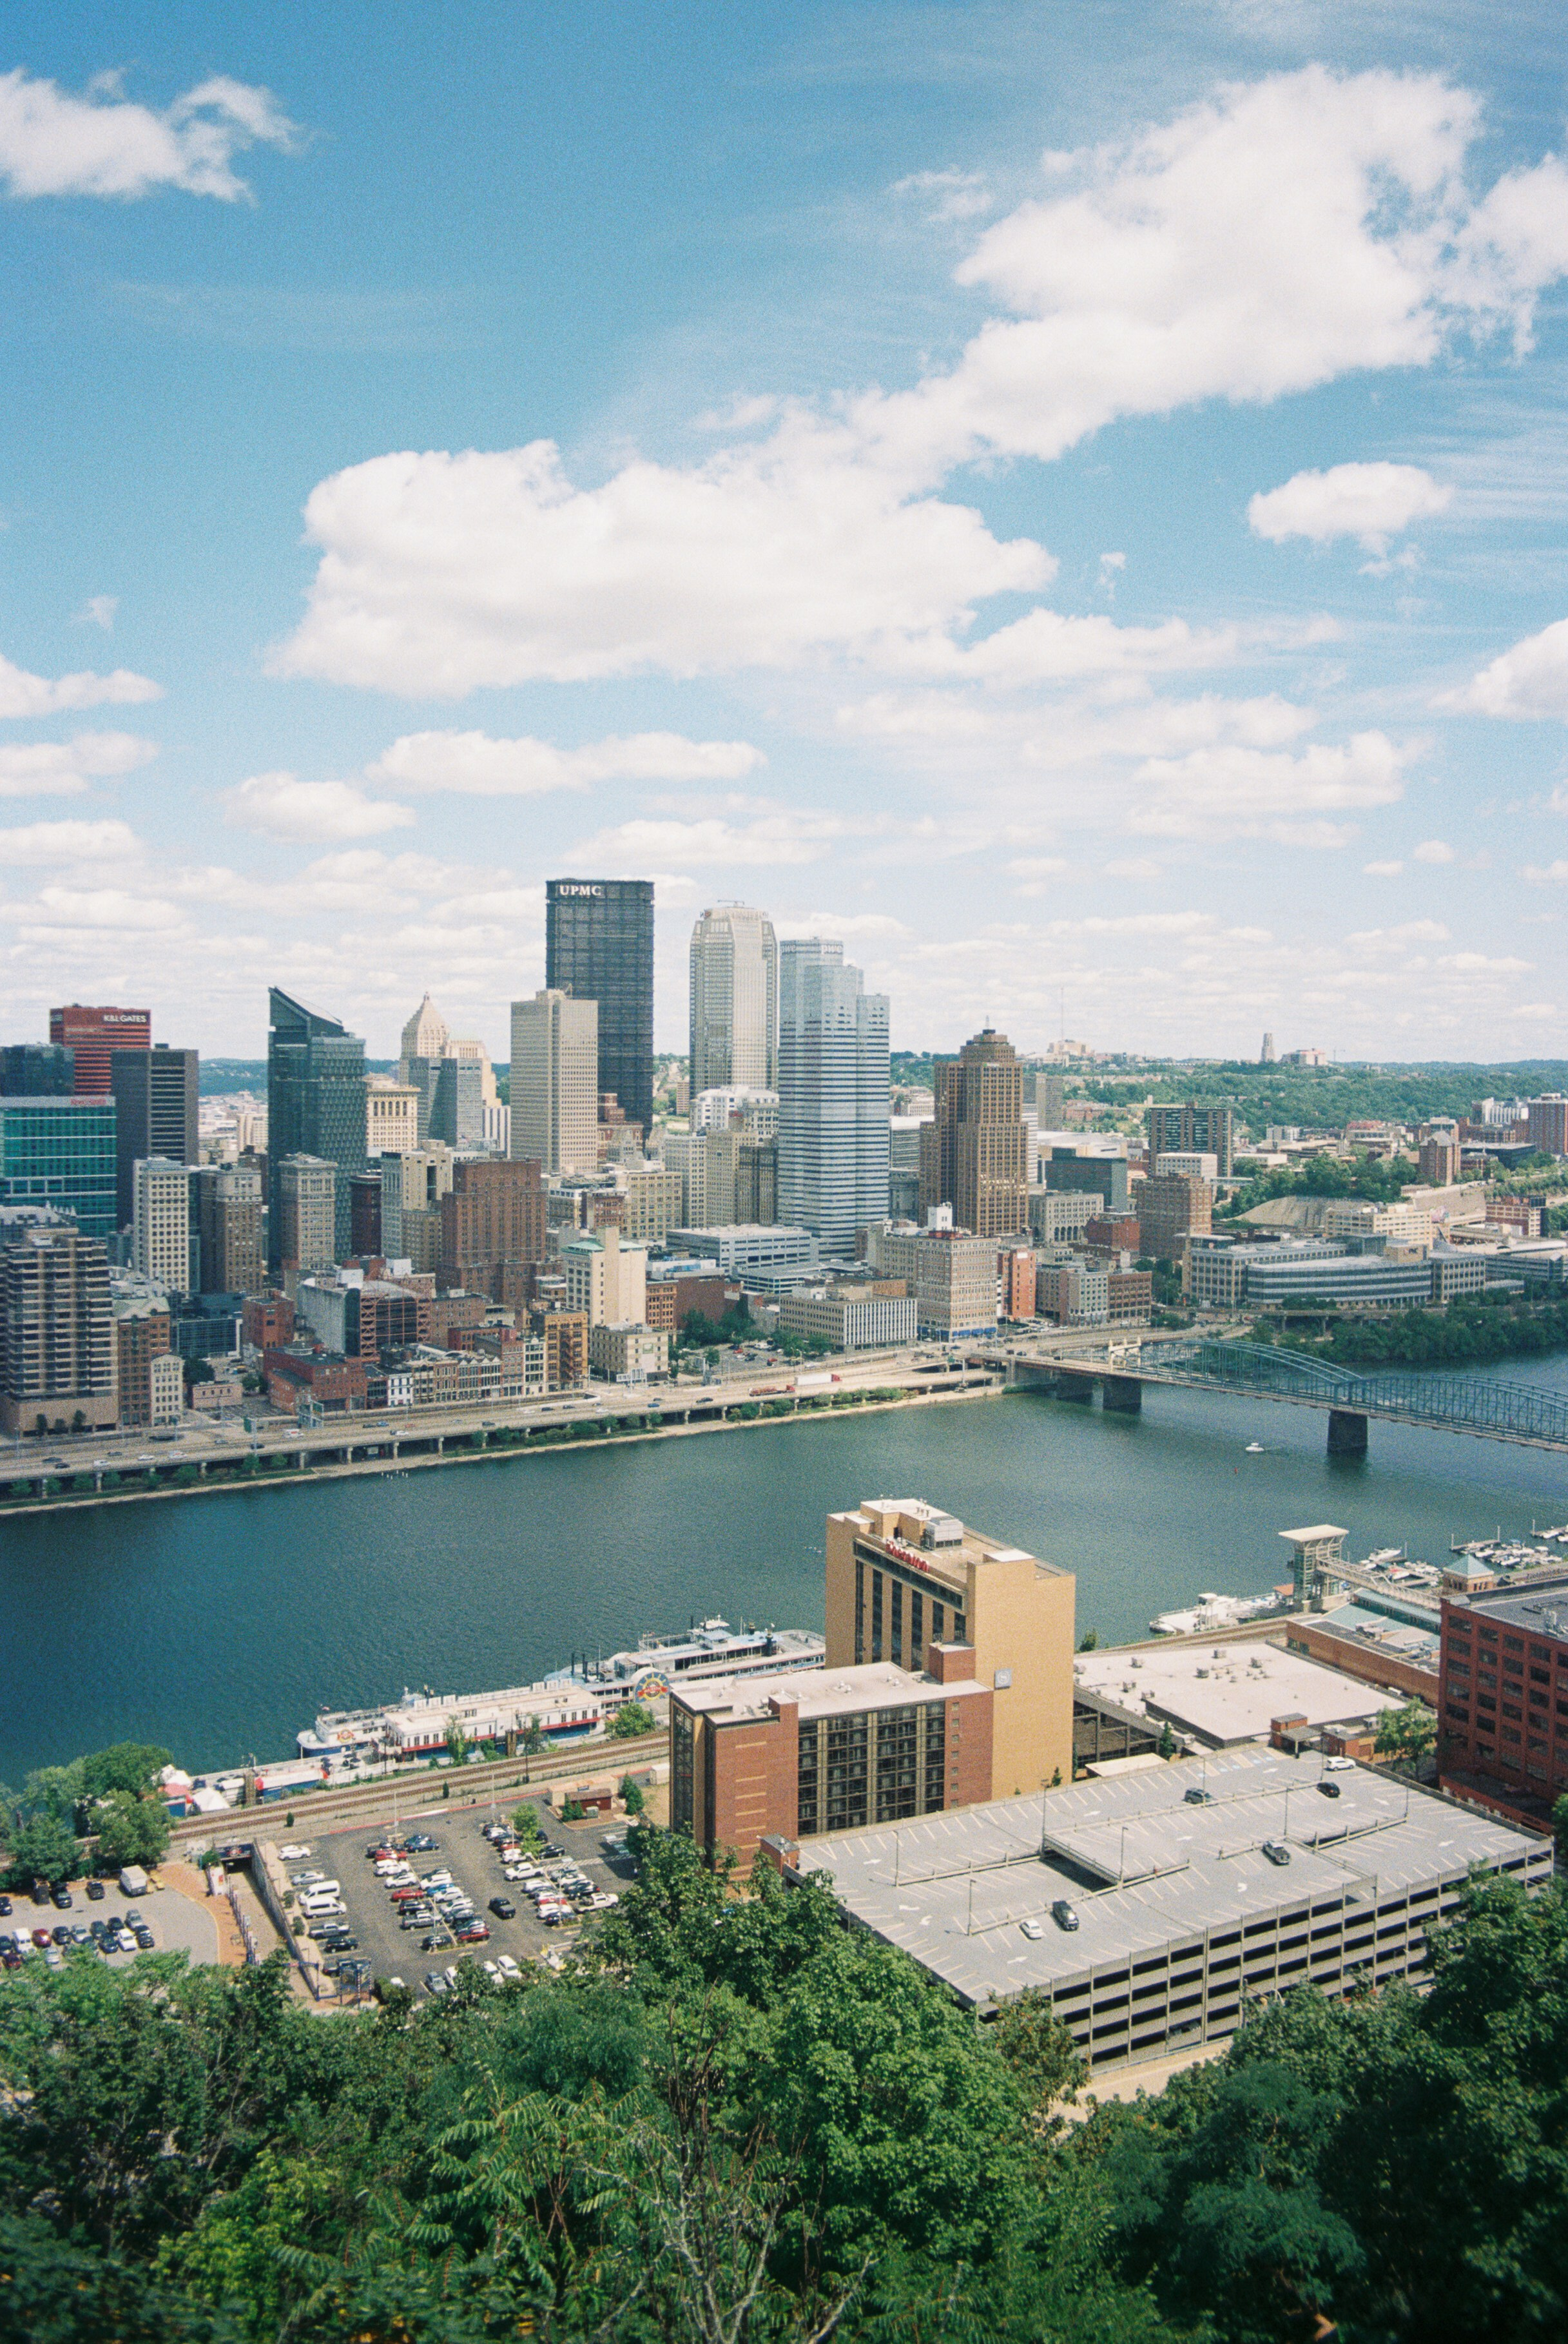
\includegraphics[scale=0.385]{./Images/banner.jpg}}} % Image background
\centering
\vspace*{5cm}
\par\normalfont\fontsize{35}{35}\sffamily\selectfont
\textbf{MAT389H1 Fall 2024}\\
{\LARGE Complex Analysis}\par % Book title
\vspace*{1cm}
{\Huge Nasrudeen Oladimeji}\par % Author name
\endgroup

%----------------------------------------------------------------------------------------
%	COPYRIGHT PAGE
%----------------------------------------------------------------------------------------

\newpage
~\vfill
\thispagestyle{empty}

%\noindent Copyright \copyright\ 2014 Andrea Hidalgo\\ % Copyright notice

\noindent\textsc{University of Toronto}\\

\noindent \textsc{github.com/Nasr-905}\\ % URL

\noindent Professor: Tristan Collins (tristan.collins@utoronto.ca)\\ % License information

\noindent \textit{First release, September 2024} % Printing/edition date

%----------------------------------------------------------------------------------------
%	TABLE OF CONTENTS
%----------------------------------------------------------------------------------------

\chapterimage{./Images/head1.jpg} % Table of contents heading image

\pagestyle{empty} % No headers

\tableofcontents % Print the table of contents itself

%\cleardoublepage % Forces the first chapter to start on an odd page so it's on the right

\pagestyle{fancy} % Print headers again

\chapterimage{./Images/head2.jpg} % Chapter heading image
\chapter{Complex Numbers}
\section{Introduction}
\begin{definition}
    [Complex Numbers]
    $z$ is a complex number iff $z = a + bi$ where $a, b \in \mathbb{R}$ and $i^2 = -1$. \\
    The set of complex numbers is denoted by $\mathbb{C}$.
\end{definition}
\begin{definition}
    [Real and Imaginary Parts]
    If $z = a + bi$, then $\Re(z) = a \in \mathbb{R}$ and $\Im(z) = b \in \mathbb{R}$. where $\Re(z)$ is the real part of $z$ and $\Im(z)$ is the imaginary part of $z$.
\end{definition}

\begin{definition}
    [Modulus]
    If $z = a + bi$, then $|z| = \sqrt{a^2 + b^2}$. $|z|$ is the modulus of $z$.
\end{definition}

\begin{definition}
    [Conjugate]
    If $z = a + bi$, then $\overline{z} = a - bi$. $\overline{z}$ is the conjugate of $z$.
\end{definition}
\section{Operations}
\begin{definition}
    [Addition and Subtraction]
    If $z_1 = a_1 + b_1i$ and $z_2 = a_2 + b_2i$, then $z_1 + z_2 = (a_1 + a_2) + (b_1 + b_2)i$. \\
    Similarly $z_1 - z_2 = (a_1 - a_2) + (b_1 - b_2)i$.
\end{definition}

\begin{definition}
    [Multiplication]
    If $z_1 = a_1 + b_1i$ and $z_2 = a_2 + b_2i$, then $z_1 \cdot z_2 = (a_1a_2 - b_1b_2) + (a_1b_2 + a_2b_1)i$. \\
    \textit{    Note that $|z_1 \cdot z_2| = |z_1| \cdot |z_2|$.}
\end{definition}

\begin{definition}
    [Inversion]
    If $z = a + bi$, then $z^{-1} = \frac{\overline{z}}{|z|^2}= \frac{a}{a^2 + b^2} - \frac{b}{a^2 + b^2}i$.
\end{definition}
\begin{proof}
    Let's multiply by 1 in the form of the conjugate of $z$:
    \begin{align*}
        \frac{1}{z} = \frac{1}{z}\times \frac{\overline{z}}{\overline{z}} = \frac{\overline{z}}{z\overline{z}} = \frac{a - bi}{(a + bi)(a - bi)} = \frac{a - bi}{a^2 + b^2} = \frac{a}{a^2 + b^2} - \frac{b}{a^2 + b^2}i
    \end{align*}
\end{proof}

\begin{definition}
    [Division]
    For $z, w \in \mathbb{C}$, $\frac{w}{z} = w \cdot z^{-1} = \frac{w\overline{z}}{|z|^2}$.
\end{definition}
\begin{table}[htbp]
    \centering
    \caption{Properties of the Complex Conjugate}
    \begin{tabular}{|c|c|}
        \hline
        \textbf{Property}        & \textbf{Description}                                                              \\
        \hline
        Conjugate of the Sum     & $\overline{z_1 + z_2} = \overline{z_1} + \overline{z_2}$                          \\
        \hline
        Conjugate Modulus        & $ z \cdot \overline{z}= |z|^2$                                                    \\
        \hline
        Conjugate of a Conjugate & $\overline{\overline{z}} = z$                                                     \\
        \hline
        Product of Conjugates    & $\overline{z_1 \cdot z_2} = \overline{z_1} \cdot \overline{z_2}$                  \\
        \hline
        Conjugate of a Quotient  & $\overline{\left(\frac{z_1}{z_2}\right)} = \frac{\overline{z_1}}{\overline{z_2}}$ \\
        \hline
        Real Part Conjugate      & $Re(z) = \frac{z + \overline{z}}{2}$                                              \\
        \hline
        Imaginary Part Conjugate & $Im(z) = \frac{z - \overline{z}}{2i}$                                             \\
        \hline
        Real Number Check        & $z = \overline{z} \iff z \in \mathbb{R}$                                          \\
        \hline
        Imaginary Number Check   & $z = -\overline{z} \iff z \in \mathbb{I}$                                         \\
        \hline
        Function Linearity       & If $\alpha = f(z)$ then $\overline{\alpha} = \overline{f(z)} = f(\overline{z})$   \\
        \hline
    \end{tabular}
\end{table}

\begin{table}[htbp]
    \centering
    \caption{Properties of the Modulus in Complex Numbers}
    \begin{tabular}{|c|c|}
        \hline
        \textbf{Property}         & \textbf{Description}                                                           \\
        \hline
        Positivity                & $|z| \geq 0$, with equality if and only if $z = 0$                             \\
        \hline
        Triangle Inequality       & $||z_1| - |z_2|| \leq |z_1 \pm z_2| \leq |z_1| + |z_2|$                        \\
        \hline
        Multiplicative Property   & $|z_1 \cdot z_2| = |z_1| \cdot |z_2|$                                          \\
        \hline
        Division Property         & $\left|\frac{z_1}{z_2}\right| = \frac{|z_1|}{|z_2|}$, for $z_2 \neq 0$         \\
        \hline
        Conjugate                 & $|z| = |\overline{z}|$                                                         \\
        \hline
        Component Property        & $-|z| \leq Re(z) \leq |z|$                                                     \\ & $-|z| \leq Im(z) \leq |z|$ \\
        \hline
        Cauchy-Schwarz Inequality & $|z_1w_1 + \cdots + z_nw_n|^2 \leq \sum_{j=1}^{n}|z_j|^2\sum_{j=1}^{n}|w_j|^2$ \\
        \hline
    \end{tabular}
\end{table}

\begin{proof}
    Proof of the Multiplicative Property of the Modulus:
    \begin{align*}
        |z_1 \cdot z_2|^2 & = (z_1 \cdot z_2) \cdot (\overline{z_1} \cdot \overline{z_2}) \\
                          & = z_1 \cdot \overline{z_1} \cdot z_2 \cdot \overline{z_2}     \\
                          & = |z_1|^2 \cdot |z_2|^2
    \end{align*}
\end{proof}
\section{Polar Representation}
A complex number are vectors in $\mathbb{R}^2$, as such, they can be represented by a magnitude and a direction. \\

\begin{definition}[Polar Form]
    \begin{align}
         & z = r(\cos(\theta) + i\sin(\theta)) \label{polar} \\
         & : r = |z| \in \mathbb{R}^+ \notag
        \label{polar form}
    \end{align}
\end{definition}

\begin{figure}[htbp]
    \centering
    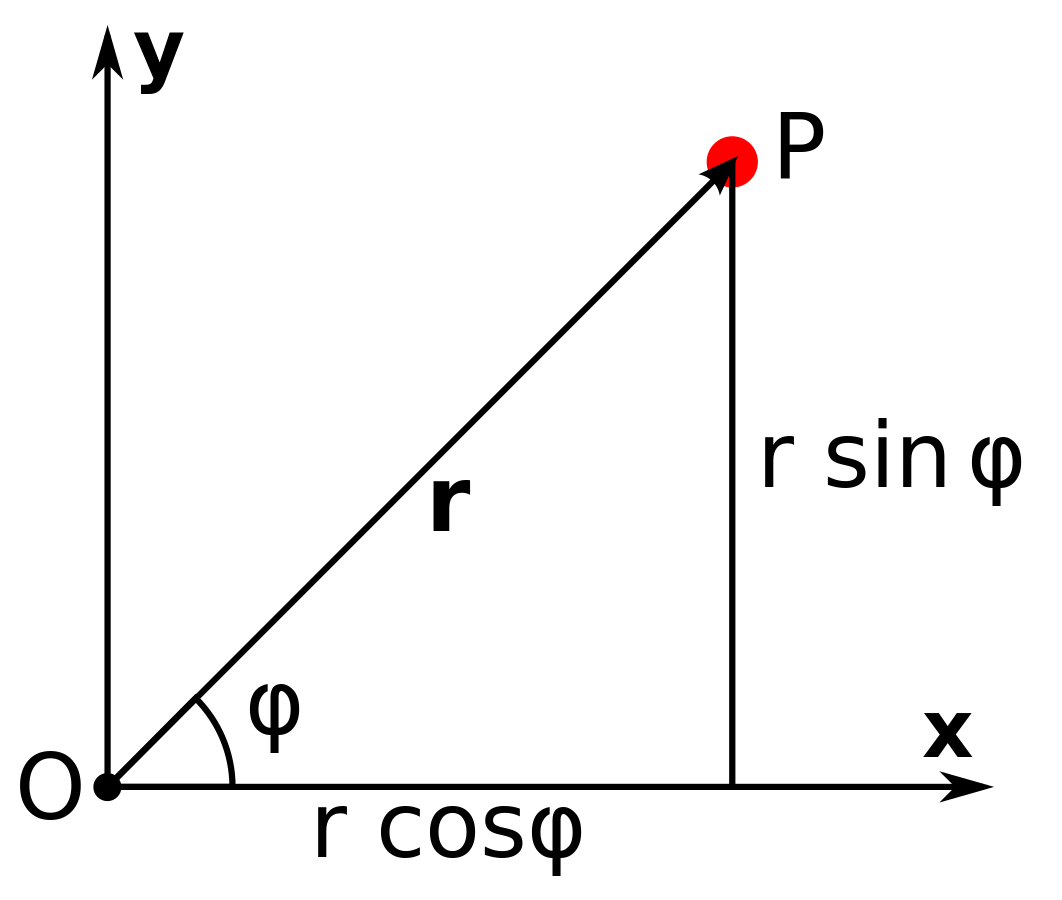
\includegraphics[scale = 0.2]{./LECTURE_1/Polar_coordinate_components.png}
    \caption{Polar Coordinate Components}
    \label{fig:polar}
\end{figure}

\begin{example}
    [Multiplying Complex Numbers in Polar Form]
    Let $z_1 = r_1(\cos(\theta_1) + i\sin(\theta_1))$ and $z_2 = r_2(\cos(\theta_2) + i\sin(\theta_2))$. Then:
    \begin{align}
        z_1 \cdot z_2 & = r_1r_2(\cos(\theta_1)\cos(\theta_2) - \sin(\theta_1)\sin(\theta_2) + i(\cos(\theta_1)\sin(\theta_2) + \sin(\theta_1)\cos(\theta_2))) \\
                      & = r_1r_2(\cos(\theta_1 + \theta_2) + i\sin(\theta_1 + \theta_2))
        \label{polar product}
    \end{align}
    Using the trig addition formula:
    \[\cos(\alpha + \beta) = \cos(\alpha)\cos(\beta) - \sin(\alpha)\sin(\beta)$ and $\sin(\alpha + \beta) = \cos(\alpha)\sin(\beta) + \sin(\alpha)\cos(\beta).\]
\end{example}

\begin{theorem}[De Moivre's Theorem]
    if $z = r(\cos(\theta) + i\sin(\theta))$
    \begin{align}
        z^n = r^n(\cos(\theta n) + i\sin(\theta n)) \label{Moivre}
    \end{align}
\end{theorem}

\begin{proof}
    \textit{The following proof will illustrative the steps to inductive reasoning}\\
    Case of $n = 1$: $z^n = r^n(\cos(\theta n) + i\sin(\theta n)) = z = r(\cos(\theta) + i\sin(\theta))$ \\
    This is true by definition. \\
    Assume that: \\
    $z^{n-1} = r^{n-1}(\cos(\theta (n-1)) + i\sin(\theta (n-1)))$ \\
    Then from Equation \eqref{polar product} we can verify: \\
    \begin{align}
        zz^{n-1} & = rr^{n-1}(\cos(\theta (n-1) + \theta) + i\sin(\theta (n-1) + \theta)) \notag \\
        z^{n}    & = r^{n}(\cos(\theta n) + i\sin(\theta n)) \notag
    \end{align}
\end{proof}

\begin{definition}
    [Argument]
    The argument of a complex number $z = r(\cos(\theta) + i\sin(\theta))$ is any angle, $\arg(z) = \theta$, such that $z = r(\cos(\theta) + i\sin(\theta))$.
\end{definition}

From Equation \eqref{polar}, we observe that $r$ is unique (because we constrained it to just positive values). $\theta$, however, is not unique.

\begin{definition}[Principle Orientation]
    We say $\theta$ is the principle orientation of $z$ if $\theta \in [-\pi, \pi)$ \\
    In this range, $\theta$ is unique.
\end{definition}

\begin{definition}
    [Vector Dot Product] The dot product of two vectors $a = (a_1, a_2)$ and $b = (b_1, b_2)$ is given by:
    \begin{align}
        a \cdot b  = \Re(a\overline{b})
        \label{dot product}
    \end{align}
    \begin{align}
        \cos \theta = \frac{a \cdot b}{|a||b|}
    \end{align}
\end{definition}

\begin{corollary}
    [Perpendicular Vectors]
    Complex variables $z$ and $w$ are perpendicular if $\Re(z\overline{w}) = 0$.
\end{corollary}

\begin{remark}
    [Complex Numbers to Solve Polynomial Equations]
    Over $\mathbb{C}$, every equation of the form $z^n = a$ has $n$ solutions.
\end{remark}
\begin{example}
    [Solving $z^n = -1$]
    Let $z = r(\cos(\theta) + i\sin(\theta))$. Then:
    \begin{align*}
        z^n               & = r^n(\cos(\theta n) + i\sin(\theta n)) = -1                                                               \\
        \implies r^n      & = 1 \text{ and } \cos(\theta n) + i\sin(\theta n) = -1                                                     \\
        \implies r        & = 1 \text{ and } \cos(\theta n) = -1 \text{ and } \sin(\theta n) = 0                                       \\
        \implies \theta n & = \pi + 2\pi k \text{ for } k \in \mathbb{Z}                                                               \\
        \implies \theta   & = \frac{\pi + 2\pi k}{n} \text{ for } k \in \mathbb{Z}                                                     \\
                          & \text{We can now find the principle solutions for } Z                                                      \\
                          & \therefore \theta_0 = \frac{\pi}{n}, \theta_1 = \frac{3\pi}{n}, \ldots, \theta_{n-1} = \frac{(2n-1)\pi}{n}
    \end{align*}
\end{example}
\begin{remark}
    Roots of Unity
    The solutions to $z^n = 1$ are called the $n$th roots of unity. Plotting these solutions splits the complex plane into $n$ equal parts.
    \begin{figure}
        \centering
        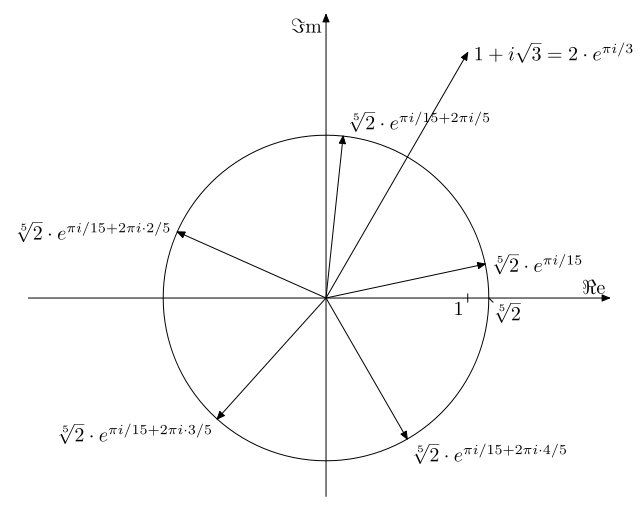
\includegraphics[scale = 0.2]{./LECTURE_1/Complex_fifth_roots.png}
        \caption{Complex Fifth Roots of Unity}
        \label{fig:roots}
    \end{figure}
\end{remark}
\section{Subsets of the Plane}
\begin{definition}
    [Open Disc]
    An open disc of radius $R$ centered at $z_0$ is the set of all $z$ such that $D_R(z_0) = \{z \in \mathbb{C} : |z - z_0| < R \subset \mathbb{C}\}$.
\end{definition}
\begin{definition}
    [Interior Point]
    A point $z_0$ is an interior point of a set $A \subset \mathbb{C}$ if there exists an open disc centered at $z_0$ that is contained in $A$.
    \[z_0 \text{is an interior point of $A$ if} \exists D_{>0}(z_0)\in A\]
\end{definition}

\begin{definition}
    [Open Set]
    A set $A \subset \mathbb{C}$ is open if every point in $A$ is an interior point. \\
    \textit{I.e. there are no 'hard lines' in the set.}
\end{definition}

\begin{example}
    [Open Disc]
    Show that the disc $D_R(z_0) = \{z \in \mathbb{C} : |z - z_0| < R\}$ is an open set.
    \begin{proof}
        Let $z_1 \in D$. Then $|z_1 - z_0| < R$. Let $r = R - |z_1 - z_0|$. Then $r > 0$. \\
        Let $z_2 \in D$ be any point in $D$, such that $|z_2 - z_1| < r$. Then:
        \begin{align*}
            |z_2 - z_0| & \leq |z_2 - z_1| + |z_1 - z_0| \\
                        & < r + R - r = R
        \end{align*}
        Therefore $z_2 \in D$ and $D$ is open.
    \end{proof}
\end{example}

\begin{definition}
    [Boundary ($\partial D$)]
    The boundary of a set $A$ is the set of all points $z$ such that every open disc centered at $z$ contains points in $A$ and points not in $A$. \\
    The boundary of $A$ is denoted by $\partial A$ and a boundary point $z$ is denoted by $z \in \partial A$.
    \[z_0 \text{is an boundary point of $A$ if} \exists z \in D_{R}(z_0) :z \notin A \forall R> 0\]
\end{definition}

\begin{definition}
    [Closed Set]
    A set $D$ is closed if it contains all its boundary points.
\end{definition}
\begin{remark}
    A set can be both open and closed ($\mathbb{C}, \emptyset$), open and not closed, closed and not open, or neither open nor closed.
\end{remark}
\begin{theorem}
    [Properties of Open and Closed Sets]
    \begin{enumerate}
        \item $D$ is open iff $\mathbb{C} \setminus D$ is closed.
        \item $D$ is closed iff $\mathbb{C} \setminus D$ is open.
        \item $D$ is open if and only if it contains none of its boundary points.
    \end{enumerate}
\end{theorem}

\chapter{Connectedness}
\section{Lecture 2: Connected Sets}
\begin{definition}
    [Connected Set]
    An \textit{open} set $D$ is connected if each pair of points $p, q \in D$ can be joined by a polygonal path lying entirely in $D$. That is:
    \[
        \exists P_2, P_3, \ldots, P_n \in D\quad  \text{ such that }\quad  pP_1, P_1P_2, \ldots, P_nq \in D\]
\end{definition}

\begin{remark}
    The set doesn't \textit{have} to be open, but it is easier to prove connectedness for open sets.
\end{remark}

\begin{figure}[H]
    \centering
    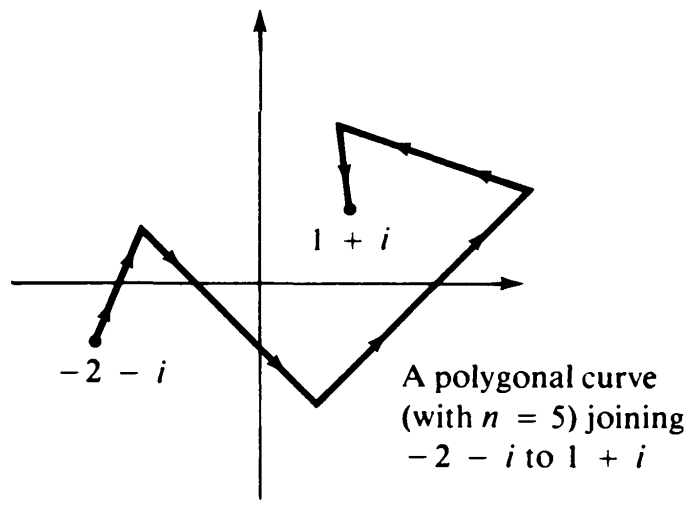
\includegraphics[scale=0.5]{LECTURE_2/poly.png}
    \caption{Polygonal Path}
    \label{fig:poly}
\end{figure}

\begin{definition}
    [Domain]
    A domain is a set that's
    \begin{itemize}
        \item Open
        \item Connected
        \item Not empty
    \end{itemize}
\end{definition}

\begin{definition}
    [Convex Set]
    A set $D$ is convex if for each pair of points $p, q \in D$, the line segment $pq$ lies entirely in $D$.
\end{definition}

\begin{figure}[H]
    \centering
    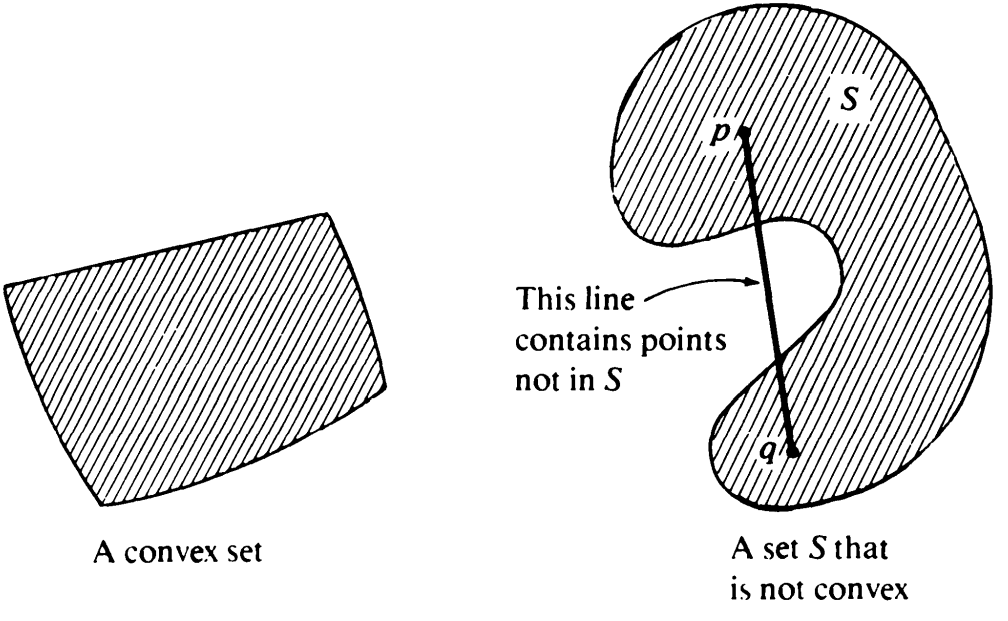
\includegraphics[scale=0.5]{LECTURE_2/convex.png}
    \caption{Convex Set}
    \label{fig:convex}
\end{figure}

\begin{theorem}
    [Convex $\implies$ Connected]
    If $D$ is a convex open set, then $D$ is connected.
\end{theorem}

\begin{definition}
    [Open Half-plane]
    A set $D$ is an open half-plane if it is of the form
    \[
        D = \{z \in \mathbb{C} : \Re\{az + b\} \geq 0\}
    \]
    \textit{Each open half-plane is convex and open}
\end{definition}

\begin{definition}
    [Closed Half-plane]
    A set $D$ is a closed half-plane if it is of the form
    \[
        D = \{z \in \mathbb{C} : \Re\{az + b\} > 0\}
    \]
    \textit{Each closed half-plane is convex and closed}
\end{definition}

\section{Point at Infinity}
\begin{definition}
    [Point at Infinity]
    A set is said to contain the point at infinity if it contains all points $z$ such that $|z| > R$ for some $R > 0$.
\end{definition}

\begin{example}
    No open Half-plane contains the point at infinity. Even though the set is unbounded, choosing $R$ near the boundary will always give a point outside the set.
\end{example}

\section{Functions and Limits}

\begin{definition}
    [Limit of a Sequence of Complex Numbers]
    \begin{align}
         & \lim_{n \to \infty} z_n = z \quad \text{or}\quad z_n \to z \iff \forall \epsilon > 0, \exists N \in \mathbb{N} \\
         & \text{such that} \quad n \geq N \implies |z_n - z| < \epsilon
    \end{align}
\end{definition}

\begin{corollary}
    [Parts of a Limit]
    If $z_n = x_n + iy_n$ and $z = x + iy$, then
    \[
        \lim_{n \to \infty} z_n = z \iff \lim_{n \to \infty} x_n = x \text{ and } \lim_{n \to \infty} y_n = y
    \]
\end{corollary}

\begin{theorem}
    [Subsequence]
    Suppose $\{z_n\}$ converges with limit $z$. Then every subsequence, $z_{m_n} = f(n)$ also converges to $z$. Where $ 1 \leq m_1 < m_2 < \ldots$
\end{theorem}

\begin{definition}
    [Limits of Functions]
    \begin{align}
         & \lim_{z \to z_0} f(z) = w \iff \forall \epsilon > 0, \exists \delta > 0 \\
         & \text{such that} 0 < |z - z_0| < \delta \implies |f(z) - w| < \epsilon
    \end{align}
\end{definition}

\section{Continuity}
\begin{definition}
    [Continuous Function]
    A function $f(z)$ is continuous at $z_0$ if
    \[
        \lim_{z \to z_0} f(z) = f(z_0)
    \]
\end{definition}

\begin{corollary}
    [Continuous at Infinity]
    A function $f(z)$ can be continuous at $\infty$ if $f(\infty) = \lim_{z\to \infty}f(z) = f(\infty)$. Note, $f(\infty)$ may equal $\infty$ \\
    \textit{This is equivalent to saying that $f(1/z)$ is continuous at $z = 0$}
\end{corollary}

\chapter{Series and Sequences}

\begin{definition}
    [infinite Series]
    Suppose we have a sequence:
    \begin{equation}
        z_1, z_2, z_3, \ldots
    \end{equation}
    We can define the partial sum of the sequence as:
    \begin{equation}
        S_n = z_1 + z_2 + z_3 + \ldots + z_n
    \end{equation}
    We say $\sum_{n=1}^{\infty} z_n$ converges and has a sum $S$ if the sequence of partial sums converges to $S$:
    \begin{equation}
        \lim_{n \to \infty} S_n = S
    \end{equation}
    If $\lim_{n \to \infty} S_n$ does not exist, we say the series diverges.
\end{definition}

\begin{corollary}
    [Real and Imaginary Parts of a Series]
    If $\sum_{n=1}^{\infty} z_n$ converges, then the real and imaginary parts of the series also converge.
    \begin{equation}
        \sum_{n=1}^{\infty} z_n = \sum_{n=1}^{\infty} \Re(z_n) + i \sum_{n=1}^{\infty} \Im(z_n)
    \end{equation}
\end{corollary}

\section{Tests for Convergence}
\begin{theorem}
    If $\sum_{n=1}^{\infty} z_n$ converges, then so does $\sum_{n=1}^{\infty} z_n$ and:
    \[
        \left| \sum_{n=1}^{\infty} z_n \right| \leq \sum_{n=1}^{\infty} |z_n|
    \]
\end{theorem}

\begin{proof}
    Say $z_n = x_n + i y_n$. Then:
    \begin{align}
         & \left| \sum_{n=1}^{\infty} x_n \right| & \leq \sum_{n=1}^{\infty}  \left| x_n \right| \leq \sum_{n=1}^{\infty}  \left| z_n \right| \\
         & \text{And}                                                                                                                         \\
         & \left| \sum_{n=1}^{\infty} y_n \right| & \leq \sum_{n=1}^{\infty}  \left| y_n \right| \leq \sum_{n=1}^{\infty}  \left| z_n \right|
    \end{align}
    So if $\sum_{n=1}^{\infty} x_n$ and $\sum_{n=1}^{\infty} y_n$ converge, then $\sum_{n=1}^{\infty} z_n$ converges.
\end{proof}

\begin{table}[htbp]
    \centering
    \begin{tabular}{| m{3cm} | m{7cm} | m{4cm} |}
        \hline
        \textbf{Test Name}         & \textbf{Description}                                                                                                                   & \textbf{Conditions for Use}                                         \\
        \hline
        Ratio Test                 & Uses the limit of the ratio of successive terms to determine convergence. \[ \lim_{n \to \infty} \left| \frac{a_{n+1}}{a_n} \right| \] & Applicable when terms are positive and the limit exists.            \\
        \hline
        Root Test                  & Uses the limit of the nth root of the terms to determine convergence. \[ \lim_{n \to \infty} \sqrt[n]{|a_n|} \]                        & Applicable when terms are positive and the limit exists.            \\
        \hline
        Integral Test              & Compares a series to an improper integral to determine convergence. \[ \int_{1}^{\infty} f(x) \, dx \]                                 & Applicable when terms are positive, continuous, and decreasing.     \\
        \hline
        Comparison Test            & Compares a series to a known convergent or divergent series.                                                                           & Applicable when terms are positive.                                 \\
        \hline
        Limit Comparison Test      & Compares the limit of the ratio of terms to a known series. \[ \lim_{n \to \infty} \frac{a_n}{b_n} \]                                  & Applicable when terms are positive and the limit exists.            \\
        \hline
        Alternating Series Test    & Determines convergence for series with alternating positive and negative terms.                                                        & Applicable when terms decrease in absolute value and approach zero. \\
        \hline
        p-Series Test              & Determines convergence based on the exponent in a series of the form \[ \sum \frac{1}{n^p} \]                                          & Applicable for series of the form \(\frac{1}{n^p}\).                \\
        \hline
        Geometric Series Test      & Determines convergence for geometric series. \[ \sum ar^n \]                                                                           & Applicable for series of the form \(ar^n\).                         \\
        \hline
        D'Alembert's Ratio Test    & Similar to the Ratio Test, but specifically for series with factorial terms.                                                           & Applicable when terms involve factorials.                           \\
        \hline
        Cauchy's Condensation Test & Determines convergence by condensing the series. \[ \sum a_n \sim \sum 2^n a_{2^n} \]                                                  & Applicable for series with positive, decreasing terms.              \\
        \hline
    \end{tabular}
    \caption{Common Tests for Convergence of Series}
    \label{table:convergence_tests}
\end{table}


\begin{example}
    \begin{align}
        \sum_{j=1}^{\infty} j \left( \frac{1 + 2i}{3} \right)^j &
    \end{align}
    We can use the ratio test to determine convergence:
    \begin{align}
        \sum_{j=1}^{\infty} \left| z_j \right|                 & = \sum_{j=1}^{\infty} j \left| \frac{1 + 2i}{3} \right|^j                                 \\
                                                               & = \sum_{j=1}^{\infty} j \left( \frac{\sqrt{5}}{3} \right)^j                               \\
        \lim_{j \to \infty} \left| \frac{z_{j+1}}{z_j} \right| & = \lim_{j \to \infty} \frac{(j+1)({\frac{\sqrt{5}}{3}})^{j + 1}}{j(\frac{\sqrt{5}}{3})^j} \\
                                                               & = \lim_{j \to \infty} \frac{j+1}{j} \left( \frac{\sqrt{5}}{3} \right)                     \\
                                                               & = \frac{5}{3} < 1
                                                               & \therefore \text{The series converges}
    \end{align}
\end{example}

\section{The Exponential Function}
\subsection*{Approach 1}
\begin{definition}
    [Exponential Function]
    If $z = x + iy$, then the exponential function is defined as:
    \begin{equation}
        e^z = e^x \left( \cos(y) + i \sin(y) \right)
    \end{equation}
\end{definition}

\begin{remark}
    [Euler's Formula]
    \begin{align}
        e^{i\theta} & \triangleq \cos(\theta) + i \sin(\theta) \\
    \end{align}
\end{remark}

\subsection*{Properties of the complex Exponential Function}
\begin{table}[htbp]
    \centering
    \begin{tabular}{| m{2.5cm} | m{11.5cm} |}
        \hline
        \textbf{Property} & \textbf{Description}                                                                                                                      \\
        \hline
        Periodicity       & The complex exponential function is periodic with period \( 2\pi i \), \[ e^{z + 2\pi i} = e^z \].                                        \\
        \hline
        Multiplication    & The exponential function satisfies \[ e^{z_1 + z_2} = e^{z_1} e^{z_2} \] for any complex numbers \( z_1 \) and \( z_2 \).                 \\
        \hline
        Derivative        & The derivative of the exponential function is \[ \frac{d}{dz} e^z = e^z \].                                                               \\
        \hline
        Inverse           & The inverse of the exponential function is the complex logarithm, \[ \log z \], such that \[ e^{\log z} = z \] for \( z \neq 0 \).        \\
        \hline
        Magnitude         & The magnitude of the exponential function is \[ |e^z| = e^{\Re(z)} \], where \( \Re(z) \) denotes the real part of \( z \).               \\
        \hline
        Argument          & The argument of the exponential function is \[ \arg(e^z) = \Im(z) \mod 2\pi \], where \( \Im(z) \) denotes the imaginary part of \( z \). \\
        \hline
        Conjugate         & The conjugate of the exponential function is \[ \overline{e^z} = e^{\overline{z}} \].                                                     \\
        \hline
    \end{tabular}
    \caption{Properties of the Complex Exponential Function}
    \label{table:complex_exponential_properties}
\end{table}

\subsection*{Approach 2: Taylor Series}

\begin{definition}
    [The Exponential Function]
    The exponential function can be defined as:
    \begin{equation}
        e^z = \sum_{n=0}^{\infty} \frac{z^n}{n!} \qquad \text{for all } z \in \mathbb{C}
    \end{equation}
\end{definition}

\begin{claim}
    [The Taylor Series for the Exponential Function Converges]
    $\sum_{n=0}^{\infty} \frac{z^n}{n!}$ converges for all $z \in \mathbb{C}$.
\end{claim}
\begin{proof}
    HOMEWORK
\end{proof}

\begin{problem}
For $\theta \in \mathbb{R}$
\[
    e^{i\theta} = \sum_{n=0}^{\infty} \frac{(i\theta)^n}{n!} = \cos(\theta) + i \sin(\theta)
\]
\end{problem}

\section{Approach 3: Differential Equations}
\begin{definition}
    [Differential Equation for the Exponential Function]
    The exponential function satisfies the differential equation:
    \begin{equation}
        f(z) = \begin{cases}
            \frac{df}{dz} = f & \text{for all } z \in \mathbb{C} \\
            f(0) = 1
        \end{cases}
    \end{equation}
\end{definition}

\section{The Logarithm Function}
\begin{definition}
    [Logarithm Function]
    The logarithm function is defined as the inverse of the exponential function:
    \begin{equation}
        \log z = \log |z| + i \theta
    \end{equation}
\end{definition}
\begin{remark}
    There will be many solutions to the logarithm function, as the argument is only defined modulo \(2\pi\).
    \[
        \log z = \log |z| + i \left( \arg(z) + 2\pi n \right) \qquad \text{for } n \in \mathbb{Z}
    \]
\end{remark}

\begin{definition}
    [Principal Logarithm]
    The principal branch logarithm is defined as:
    \[
        \text{Log}(z) = \log |z| + i \arg(z) \qquad \text{for } -\pi < \arg(z) \leq \pi
    \]
    \textit{Note: We use a capital L to denote the principal logarithm.}
\end{definition}

\begin{definition}
    [Fixed $\theta_0$ Logarithm Function]
    We can fix the argument of the logarithm function by setting \(\theta_0\) and letting $D = \{ te^{i\theta_0} | t > 0, t \in \mathbb{R} \}$.\\
    We define:
    \[
        \widetilde{\log}_{\theta_0} z = \log |z| + i \left( \widetilde{\arg}(z) + \theta_0 \right) \qquad \text{for } z \in D, \arg(z) \in [\theta_0, \theta_0 + 2\pi)
    \]
\end{definition}

\begin{example}
    [Find the Values of $(-1)^i$]
    \begin{align}
        (-1)^i   & = e^{i \log(-1)}                         \\
                 & = e^{i (2n + 1)\pi i}                    \\
                 & = e^{-2n\pi}                             \\
        \log(-1) & = -(2n + 1)\pi i \qquad n \in \mathbb{Z} \\
        (-1)^i   & = e^{2n + 1}\pi
    \end{align}
\end{example}

\section{The Trigonometric Functions}
\begin{definition}
    [Trigonometric Functions]
    For $z \in mathbb{C}$ trigonometric functions are defined as:
    \begin{align}
        \Re{e^{iz}} & = \cos(z)  = \frac{e^{iz} + e^{-iz}}{2}  \\
        \Im{e^{iz}} & = \sin(z)  = \frac{e^{iz} - e^{-iz}}{2i} \\
        \tan(z)     & = \frac{\sin(z)}{\cos(z)}                \\
    \end{align}
\end{definition}

\begin{lemma}
    \begin{align}
        \begin{cases}
            \cos(z + \alpha) = \cos(z) \\
            \sin(z + \alpha) = \sin(z)
        \end{cases}
    \end{align}
    iff $\alpha = 2\pi n$ for $n \in \mathbb{Z}$.
\end{lemma}

\begin{proof}
    \begin{align}
        e^{i(z + \alpha)} & = e^{iz} e^{i\alpha}                                   \\
                          & = e^{iz} \left( \cos(\alpha) + i \sin(\alpha) \right)  \\
                          & = e^{iz} \left( \cos(2\pi n) + i \sin(2 \pi n) \right) \\
                          & = e^{iz}
    \end{align}
\end{proof}

\chapter{Homework 1}

\begin{example}
    [Fisher, Section 1.2, Problem 2] Describe the locus of points $z$ satisfying the equation
    \[|z-4|=4|z|\]
    \textbf{Solution:} \\
    Let $z=x+iy$. Then
    \begin{align*}
        |z-4|                                     & = |x+iy-4| = |x-4+iy| = \sqrt{(x-4)^2+y^2}                                   \\
        4|z|                                      & = 4|x+iy| = 4\sqrt{x^2+y^2}                                                  \\
        \sqrt{(x-4)^2+y^2}                        & = 4\sqrt{x^2+y^2}                                                            \\
        (x-4)^2+y^2                               & = 16(x^2+y^2)                                                                \\
        x^2-8x+16+y^2                             & = 16x^2+16y^2                                                                \\
        15x^2+15y^2+8x-16                         & = 0                                                                          \\
        x^2 + y^2 + \frac{8}{15}x - \frac{16}{15} & = 0                                                                          \\
        \Rightarrow \quad \text{complete the square}                                                                             \\
        x^2                                       & + \frac{8}{15}x + (\frac{4}{15})^2 - (\frac{4}{15})^2 + y^2  = \frac{16}{15} \\
        (x+\frac{4}{15})^2 + y^2                  & = \frac{16}{15} + (\frac{4}{15})^2                                           \\
        (x+\frac{4}{15})^2 + y^2                  & = \frac{16}{15} + \frac{16}{225}                                             \\
        (x+\frac{4}{15})^2 + y^2                  & = \frac{256}{225}                                                            \\
    \end{align*}
    $\therefore$ The locus of points $z$ satisfying the equation $|z-4|=4|z|$ is a circle with center $(-\frac{4}{15},0)$ and radius $\sqrt{\frac{256}{225}} = \frac{16}{15}$.
\end{example}

\begin{example}
    [Fisher, Section 1.2, Problem 24]
    Find all solutions of the equation
    \[(z+1)^4=1-i\]
    \textbf{Solution:} \\
    \begin{align*}
                    & \quad \text{Convert $1-i$ to polar form}                                                           \\
        \arg{1-i}   & = \tan^{-1}(-1) = -\frac{\pi}{4} + 2k\pi        \quad \text{where $k\in\mathbb{Z}$}                \\
        |1-i|       & = \sqrt{1^2+(-1)^2} = \sqrt{2}                                                                     \\
        1-i         & = \sqrt{2}(cos(-\frac{\pi}{4} + 2k\pi)+isin(-\frac{\pi}{4} + 2k\pi))                               \\
                    & \quad \text{Use De Moivre's Theorem}                                                               \\
        \rightarrow & z^n = r^n(cos(n\theta)+isin(n\theta))                                                              \\
        z +1        & = 2^{\frac{1}{8}}(\cos(\frac{-\pi}{4}+\frac{2\pi k}{4})+i\sin(\frac{-\pi}{4}+\frac{2\pi k}{4}))    \\
        z           & = 2^{\frac{1}{8}}(\cos(\frac{-\pi}{4}+\frac{2\pi k}{4})+i\sin(\frac{-\pi}{4}+\frac{2\pi k}{4})) -1 \\
    \end{align*}
    We can now find the solutions by plugging in $k=0,1,2,3$.
    \begin{align}
        \theta_0 & = \frac{-\pi}{4} + \frac{2\pi \cdot 0}{4} = -\frac{\pi}{4} \quad k = 0 \nonumber \\
        \theta_1 & = \frac{-\pi}{4} + \frac{2\pi \cdot 1}{4} = \frac{\pi}{4} \quad k = 1 \nonumber  \\
        \theta_2 & = \frac{-\pi}{4} + \frac{2\pi \cdot 2}{4} = \frac{3\pi}{4} \quad k = 2 \nonumber \\
        \theta_3 & = \frac{-\pi}{4} + \frac{2\pi \cdot 3}{4} = \frac{5\pi}{4} \quad k = 3 \nonumber
    \end{align}
    So our solutions are:
    \begin{align}
        z = 2^{\frac{1}{8}}(\cos(-\frac{\pi}{4})+i\sin(-\frac{\pi}{4})) -1 & = 2^{\frac{1}{8}}(\frac{\sqrt{2}}{2}-\frac{\sqrt{2}}{2}i) -1 \nonumber  \\
        z = 2^{\frac{1}{8}}(\cos(\frac{\pi}{4})+i\sin(\frac{\pi}{4})) -1   & = 2^{\frac{1}{8}}(\frac{\sqrt{2}}{2}+\frac{\sqrt{2}}{2}i) -1 \nonumber  \\
        z = 2^{\frac{1}{8}}(\cos(\frac{3\pi}{4})+i\sin(\frac{3\pi}{4})) -1 & = 2^{\frac{1}{8}}(-\frac{\sqrt{2}}{2}+\frac{\sqrt{2}}{2}i) -1 \nonumber \\
        z = 2^{\frac{1}{8}}(\cos(\frac{5\pi}{4})+i\sin(\frac{5\pi}{4})) -1 & = 2^{\frac{1}{8}}(-\frac{\sqrt{2}}{2}-\frac{\sqrt{2}}{2}i) -1 \nonumber
    \end{align}
\end{example}

\begin{example}
    [Fisher, Section 1.2, Problem 26]
    Find all solutions of the equation $z^3=8$.
    \textbf{Solution:} \\
    First, we convert $8$ to polar form.
    \begin{align*}
        8 & = 8(\cos(0)+i\sin(0))                                               \\
          & = 8(\cos(2\pi k)+i\sin(2\pi k)) \quad \text{where $k\in\mathbb{Z}$}
    \end{align*}
    Then we use De Moivre's Theorem to find the solutions.
    \begin{align*}
        \rightarrow z^n & = r^n(\cos(n\theta)+i\sin(n\theta))                                              \\
        z               & = 2(\cos(\frac{2\pi k}{3})+i\sin(\frac{2\pi k}{3})) \quad \text{where $k=0,1,2$}
    \end{align*}
    So our solutions are:
    \begin{align*}
        z = 2(\cos(0)+i\sin(0))                           & = 2(1+i0) = 2                                        \\
        z = 2(\cos(\frac{2\pi}{3})+i\sin(\frac{2\pi}{3})) & = 2(-\frac{1}{2}+i\frac{\sqrt{3}}{2}) = -1+i\sqrt{3} \\
        z = 2(\cos(\frac{4\pi}{3})+i\sin(\frac{4\pi}{3})) & = 2(-\frac{1}{2}-i\frac{\sqrt{3}}{2}) = -1-i\sqrt{3}
    \end{align*}
\end{example}

\begin{example}
    [Fisher, Section 1.3, Problem 2]
    For the following set, describe (i) the interior and the boundary, (ii) state whether the set is open, or closed, or neither open nor closed, (iii) state whether the interior of the set is connected (if it has an interior).
    $$A = \{z\in\mathbb{C}:|z|<1\text{or}|z-3|\leq1\}$$
    \textbf{Solution:} \\
    \begin{enumerate}
        \item $A_{int} = \{|z| < 1 \text{ or } |z - 3| < 1\}$
        \item $A_{bd} = \{|z| = 1 \text{ or } |z - 3| = 1\}$
        \item $A$ is neither open nor closed because $\{|z| = 1\} \notin A$ but $\{|z - 3| = 1\} \in A_{int}$, so $A$ contains only part of its boundary.
        \item $A_{int}$ is not connected, because $z_1 = 0, z_2 = 3 \in A_{int}$, but $\nexists P_1P_2\ldots P_n \in A_{int} $ such that $z_1P_1P_2\ldots P_nz_2 \in A_{int}$
    \end{enumerate}
\end{example}

\begin{example}
    [Fisher, Section 1.3, Problem 4]
    For the following set, describe (i) the interior and the boundary, (ii) state whether the set is open, or closed, or neither open nor closed, (iii) state whether the interior of the set is connected (if it has an interior).
    $$A = \{z\in\mathbb{C}:\mathrm{Re}(z^2)=4\}$$

    \textbf{Solution:} \\
    Let $z=x+iy$. Then
    \begin{align*}
        \mathrm{Re}(z^2) & = \mathrm{Re}((x+iy)^2)
        = \mathrm{Re}(x^2-y^2+2ixy)                \\
                         & 4 = x^2-y^2
    \end{align*}
    \begin{enumerate}
        \item No interior, because $\forall z_0 \in A \quad \nexists D | D_R(z_0) = \{z \in \mathbb{C} : |z - z_0| < R, R > 0\} $
        \item $A_{bd} = \{z \in \mathbb{C} : x^2 - y^2 = 4\}$
        \item $ A_{bd} = A$ so $A$ is closed.
        \item $A_{int}$ is connected because $A_{int} = \emptyset$.
    \end{enumerate}
\end{example}
\begin{figure}[h]
    \centering
    \begin{tikzpicture}
        \begin{axis}[
                axis lines = center,
                xlabel = $x$,
                ylabel = $y$,
                xmin = -5,
                xmax = 5,
                ymin = -5,
                ymax = 5,
            ]
            \addplot [
                domain=-5:5,
                samples=100,
                color=red,
            ]
            {sqrt(x^2-4)};
            \addplot [
                domain=-5:5,
                samples=100,
                color=red,
            ]
            {-sqrt(x^2-4)};
        \end{axis}

    \end{tikzpicture}
    \caption{Plot of $ 4 = x^2-y^2$}
\end{figure}

\begin{example}
    [Fisher, Section 1.4, Problem 12]
    Find
    $$\lim_{z\to2}(z-2)\log|z-2|,$$
    or explain why it does not exist.
    \textbf{Solution:} \\
    We use L'Hopital's Rule to find the limit.
    \begin{align}
        \lim_{z \to 2} (z-2)\log|z-2| & = \lim_{z \to 2} \frac{\log|z-2|}{\frac{1}{z-2}} \nonumber                                                         \\
                                      & = \lim_{z \to 2} \frac{\frac{\partial}{\partial z}\log|z-2|}{\frac{\partial}{\partial z}\frac{1}{(z-2)}} \nonumber \\
                                      & = \lim_{z \to 2} \frac{\frac{1}{z-2}}{-\frac{1}{(z-2)^2}} \nonumber                                                \\
                                      & = \lim_{z \to 2} \frac{1}{\frac{1}{2-z}} \nonumber                                                                 \\
                                      & = \lim_{z \to 2} 2-z \nonumber                                                                                     \\
                                      & = 0 \nonumber
    \end{align}
\end{example}

\begin{example}
    [Fisher, Section 1.4, Problem 16]
    Find all the points where the following function is continuous:
    $$f(z)=\begin{cases}\:\frac{z^4-1}{z-i},&z\neq i\\\:4i,&z=i\end{cases}$$
    \textbf{Solution:} \\
    First normalize the denominator.
    \begin{align*}
        f(z) & = \frac{z^4-1}{z-i} = \frac{(z^2+1)(z+1)(z-1)}{z-i} = \frac{(z^2+1)(z+1)(z-1)}{z-i}\frac{z+i}{z+i} \\
             & = \frac{(z^2+1)(z+1)(z-1)(z+i)}{z^2+1} = (z+1)(z-1)(z+i), \quad z \neq i
    \end{align*}
    As this is a polynomial, it is continuous everywhere except at $z=i$. Now we test for continuity at $z=i$.
    \begin{align*}
        \lim_{z \to i} f(z)           & = f(i) \\
        \lim_{z \to i}(z+1)(z-1)(z+i) & = 4i   \\
        (i+1)(i-1)(i+i)               & = 4i   \\
        4i                            & = 4i
    \end{align*}
    So $f(z)$ is continuous everywhere.
\end{example}


\begin{example}
    [Fisher, Section 1.4, Problem 34]
    Does the following series converge or diverge?
    $$\sum_{n=1}^\infty\frac1{2+i^n}$$
    \textbf{Solution:} \\
    We notice:
    \begin{align*}
        \frac{1}{2+i^n} & = \frac{1}{2+1} \quad \text{for $n=0, 4, 8, \ldots$} \\
        \frac{1}{2+i^n} & = \frac{1}{2+i} \quad \text{for $n=1,5,9,\ldots$}    \\
        \frac{1}{2+i^n} & = \frac{1}{2-1} \quad \text{for $n=2,6,10,\ldots$}   \\
        \frac{1}{2+i^n} & = \frac{1}{2-i} \quad \text{for $n=3,7,11,\ldots$}
    \end{align*}
    Which forms a cycle, so the series diverges.
\end{example}

\begin{example}
    [Fisher, Section 1.4, Problem 36]
    Show that each of the following series converges for all $z$.
    \begin{enumerate}
        \item $$\sum_{n=0}^\infty\frac{z^{n}}{n!}$$
        \item $$\sum_{n=0}^\infty(-1)^n\frac{z^{2n}}{(2n)!}$$
        \item $$\sum_{n=0}^\infty\frac{z^{2n+1}}{(2n+1)!}$$
    \end{enumerate}
    \textbf{Solution:} \\
    \begin{enumerate}
        \item We use the ratio test to show convergence.
              \begin{align*}
                  \lim_{n \to \infty} \left|\frac{a_{n+1}}{a_n}\right| & = \lim_{n \to \infty} \left|\frac{z^{n+1}}{(n+1)!}\frac{n!}{z^n}\right| \\
                                                                       & = \lim_{n \to \infty} \left|\frac{z}{n+1}\right|                        \\
                                                                       & = 0
              \end{align*}
              So the series converges for all $z$.
        \item We use the ratio test to show convergence.
              \begin{align*}
                  \lim_{n \to \infty} \left|\frac{a_{n+1}}{a_n}\right| & = \lim_{n \to \infty} \left|\frac{(-1)^{n+1}\frac{z^{2(n+1)}}{(2(n+1))!}}{(-1)^n\frac{z^{2n}}{(2n)!}}\right| \\
                                                                       & = \lim_{n \to \infty} \left|\frac{z^2}{(2n+2)(2n+1)}\right|                                                  \\
                                                                       & = 0
              \end{align*}
              So the series converges for all $z$.
        \item We use the ratio test to show convergence.
              \begin{align*}
                  \lim_{n \to \infty} \left|\frac{a_{n+1}}{a_n}\right| & = \lim_{n \to \infty} \left|\frac{z^{2(n+1)+1}}{(2(n+1)+1)!}\frac{(2n+1)!}{z^{2n+1}}\right| \\
                                                                       & = \lim_{n \to \infty} \left|\frac{z^2}{(2n+3)(2n+2)(2n+1)}\right|                           \\
                                                                       & = 0
              \end{align*}
              So the series converges for all $z$. \qedhere
    \end{enumerate}

\end{example}

\chapter{Line Integrals: Green's Continuous  Map}
\begin{theorem}
    [Parametrized Curves]
    $$ \gamma (t) = x(t) + iy(t) \quad a \leq t \leq b $$
    $\gamma [a,b] \to \mathbb{C}$ is the image of $\gamma$.
\end{theorem}

\begin{definition}
    [Simple Curve]
    A curve $\gamma$ is \textbf{simple} if $\gamma(t_1) = \gamma(t_2) \implies t_1 = t_2$ for $t_1, t_2 \neq a, b$.
\end{definition}
\begin{definition}
    [Closed Curve]
    A curve $\gamma$ is \textbf{closed} if $\gamma(a) = \gamma(b)$. So if the end point meets the starting point.
\end{definition}

\begin{remark}
    We can \textit{ignore} the parametrization and talk about the curve $$Image(\gamma) \subset \mathbb{C}$$ as a subset of $\mathbb{C}$.
\end{remark}

\begin{definition}
    [$C^1$/Smooth Curve]
    A parametrized curve is $C^1$ if $\gamma'(t)$ if
    $$\gamma '(t) = x'(t) + iy'(t)$$ exists $\forall t \in [a,b]$ and is continuous.
\end{definition}

\begin{remark}
    Here, $\gamma'(a), \gamma'(b)$ are the 1-sided derivatives.
\end{remark}

\begin{definition}
    [Piecewise $C^1$/Smooth Curve]
    $$\text{if } \exists a = t_0 < t_1 < \ldots < t_n = b \text{ such that } \gamma |_{[t_i, t_{i+1}]} \text{ is } C^1$$
\end{definition}

\section{Line Integrals}
\begin{definition}
    [Line Integral]
    if $g = u + iv, (u,v) \in \mathbb{R}^2$ is a complex-valued function and $\gamma$ is piecewise $C^1$, then the line integral of $g$ along $\gamma$ is
    $$\int_{\gamma} g(z) dz = \sum_{i=0}^{n-1}\int_{i}^{i+1} g(\gamma(t)) \gamma'(t) dt$$
    Where
    \begin{align*}
        g(\gamma(t)) \gamma'(t) & = ux' - vy' + ivx' + iuy'                        \\
                                & = (u(\gamma(t)) + iv(\gamma(t)))(x'(t) + iy'(t)) \\
    \end{align*}
    is complex multiplication
\end{definition}

\begin{theorem}
    [Length of a Curve]
    If $\gamma$ is a piecewise $C^1$ curve, then the length of $\gamma$ is
    $$\text{Length}(\gamma) = \sum_{i = 0}^{n-1}\int_{t_i}^{t_{i + 1}} |\gamma'(t)| dt$$
    So we have
    $$ |\int_{\gamma}g |\leq \max_{z \in \gamma}|g(z)| \cdot \text{Length}(\gamma) $$
\end{theorem}

\begin{theorem}
    [Green's Theorem]
    Say $ \Omega \subset \mathbb{C} $ such that $\partial \Omega$ is a finite collection of piecewise $C^1$ closed simple curves. If $g = u + iv$ is $C^1$ on $\Omega$, then
    % $$\int_{\partial \Omega} g = \int_{\Omega} \left( \frac{\partial v}{\partial x} - \frac{\partial u}{\partial y} \right) dxdy$$
    % Where $\partial \Omega$ is the boundary of $\Omega$.

    if $ = p + iq$ is differentiable in $\Omega$, then ($\Re{p, q}$ have $1^{st}$ order derivatives). Then
    $$\int_{\partial \Omega} f = i \int_{\Omega} \left( \frac{\partial f}{\partial x} - \frac{\partial f}{\partial y} \right) dxdy$$
    Where $\partial \Omega$ is the boundary of $\Omega$.
\end{theorem}

\begin{corollary}
    If $dz = dx + idy$, then
    \begin{align*}
        \Re(fdz) & = \Re(f)dx - \Im(f)dy \\
                 & = pdx - qdy           \\
        \Re{(i \left(\frac{\partial f}{\partial x} + \frac{i \partial f}{\partial y}\right))} = - \frac{\partial q}{\partial x} - \frac{\partial p}{\partial y}
    \end{align*}
    So
    \begin{align*}
        \int_{\partial \Omega} pdx + qdy = \left(
        \int_{\Omega} \left( \frac{\partial q}{\partial x} + \frac{\partial p}{\partial y} \right) dxdy
        \right)
    \end{align*}
\end{corollary}

\begin{remark}
    Orient $\partial \Omega$ always on the left (in the counter-clockwise direction outsides, conterclockwise insides) as we walk along $\partial \Omega$ (say $\partial \Omega$ is positively oriented).
\end{remark}

\begin{example}
    [Very Important Example]
    Let $\gamma$ be a simple, closed piecewise $C^1$ curve. such that $\gamma = \partial \Omega$ for some $\Omega \subset \mathbb{C}$. Then for $ p \notin \Omega$,
    $$ \frac{1}{2\pi i} \int_{\gamma} \frac{dz}{z - p} = \begin{cases}
            1 & \text{if } p \in \Omega    \\
            0 & \text{if } p \notin \Omega
        \end{cases} $$
    \begin{proof}
        1) Assume $p$ not in $\Omega$, then $\frac{1}{z - p}$ is differentiable in $\Omega$ and $\partial \Omega$ is a simple closed curve. So by Green's Theorem,
        $$ \int_{\partial \Omega} \frac{dz}{z - p} = i \int_{\Omega} \left( \frac{\partial}{\partial x} \frac{1}{z - p} - i\frac{\partial}{\partial y} \frac{1}{z - p} \right) dxdy = 0 $$
    \end{proof}
    Let $D_{\epsilon}(p)$ be the disk of radius $\epsilon$ centered at $p$, essentially, we want to remove the point stopping us from applying Green's Theorem.
    $$ \Omega_{\epsilon} = \Omega \setminus D_{\epsilon}(p) $$
    If $\epsilon$ is sufficiently small, $\Omega_{\epsilon}$ is still a domain. So by Green's Theorem,
    \begin{align*} \int_{\partial \Omega_{\epsilon}} \frac{dz}{z - p}                                         & = 0                                                                    \\
               \int_{\partial \Omega} \frac{dz}{z - p} - \int_{\partial D_{\epsilon}(p)} \frac{dz}{z - p} & = 0                                                                    \\
               \int_{\partial \Omega} \frac{dz}{z - p}                                                    & = \int_{\partial D_{\epsilon}(p)} \frac{dz}{z - p}                     \\
               \rightarrow \partial D_{\epsilon}                                                          & = p + \epsilon e^{it} \quad 0 \leq t \leq 2\pi                         \\
               \int_{\partial D_{\epsilon}(p)} \frac{dz}{z - p}                                           & = \int_{0}^{2\pi} \frac{i\epsilon e^{it}}{\epsilon e^{it}} dt = 2\pi i \\
               \int_{\partial \Omega} \frac{dz}{z - p}                                                    & = 2\pi i
    \end{align*}
\end{example}


\chapter{Analytic Functions and the Cauchy-Riemann Equations}

\section{Analytic Functions}

\begin{definition}
    [Complex Differentiability]
    A complex function $f(z): D \to \mathbb{C}$, where $D$ is a domain, is \textbf{complex differentiable} at $z_0 \in D$ if
    $$f'(z_0) = \lim_{z \to z_0} \frac{f(z) - f(z_0)}{z - z_0} \quad \text{exists}$$
    $$ = \lim_{h} \frac{f(z_0 + h) - f(z_0)}{h} \quad h \in \mathbb{C}$$
\end{definition}

\begin{definition}
    [Analytic]
    A function $f(z)$ is \textbf{analytic} on a domain $D$ if $f(z)$ is complex differentiable at every point in $D$.
\end{definition}

\begin{definition}
    [Entire]
    A function $f(z)$ is \textbf{entire} if $f(z)$ is analytic on $\mathbb{C}$.
\end{definition}

\begin{example}
    [Prove the Power Rule]
    $$f(z) = z^n \quad n \in \mathbb{Z}$$
    $f$ is entire and
    $$f'(z) = nz^{n-1}$$
\end{example}
\begin{proof}
    \begin{align*}
        \lim_{h \to 0} \frac{f(z + h) - f(z)}{h} & = \lim_{h \to 0} \frac{(z + h)^n - z^n}{h}                               \\
                                                 & = \lim_{h \to 0} \frac{\sum_{k=0}^{n} \binom{n}{k} z^{n-k} h^k - z^n}{h} \\
                                                 & = \lim_{h \to 0} \sum_{k=0}^{n} \binom{n}{k} z^{n-k} h^{k-1}             \\
                                                 & = \binom{n}{1} z^{n-1}                                                   \\
                                                 & = nz^{n-1}                                                               \\
    \end{align*}
\end{proof}

\begin{example}
    Prove that $f(z) = \overline{z}$ is not complex differentiable at any point.
\end{example}
\begin{proof}
    In homework 2...
\end{proof}

\begin{table}[htbp]
    \centering
    \begin{tabular}{| m{5cm} | m{9cm} |}
        \hline
        \textbf{Property}       & \textbf{Description}                                                                                                                                                                               \\
        \hline
        Linearity               & The derivative of a sum is the sum of the derivatives: \[ (f + g)'(z) = f'(z) + g'(z) \] The derivative of a constant multiple is the constant multiple of the derivative: \[ (cf)'(z) = cf'(z) \] \\
        \hline
        Product Rule            & The derivative of a product is given by: \[ (fg)'(z) = f'(z)g(z) + f(z)g'(z) \]                                                                                                                    \\
        \hline
        Quotient Rule           & The derivative of a quotient is given by: \[ \left( \frac{f}{g} \right)'(z) = \frac{f'(z)g(z) - f(z)g'(z)}{g(z)^2} \]                                                                              \\
        \hline
        Chain Rule              & The derivative of a composition is given by: \[ (f \circ g)'(z) = f'(g(z))g'(z) \]                                                                                                                 \\
        \hline
        Exponential Function    & The derivative of the exponential function is: \[ \frac{d}{dz} e^z = e^z \]                                                                                                                        \\
        \hline
        Logarithmic Function    & The derivative of the logarithmic function is: \[ \frac{d}{dz} \log z = \frac{1}{z} \]                                                                                                             \\
        \hline
        Power Rule              & The derivative of a power function is: \[ \frac{d}{dz} z^n = nz^{n-1} \]                                                                                                                           \\
        \hline
        Trigonometric Functions & The derivatives of the trigonometric functions are: \[ \frac{d}{dz} \sin z = \cos z \] \[ \frac{d}{dz} \cos z = -\sin z \]                                                                         \\
        \hline
        Hyperbolic Functions    & The derivatives of the hyperbolic functions are: \[ \frac{d}{dz} \sinh z = \cosh z \] \[ \frac{d}{dz} \cosh z = \sinh z \]                                                                         \\
        \hline
    \end{tabular}
    \caption{Properties of Complex Derivatives}
    \label{table:complex_derivative_properties}
\end{table}

\begin{example}
    [Prove the Derivative of the Exponential Function]
    $$f(z) = e^z$$
\end{example}

\begin{proof}
    \begin{align*}
        \lim_{h \to 0} \frac{e^{z + h} - e^z}{h} & = \lim_{h \to 0} \frac{e^z e^h - e^z}{h}                          \\
                                                 & = e^z \lim_{h \to 0} \frac{e^h - 1}{h}                            \\
                                                 & = e^z \lim_{h \to 0} \frac{1 + h + \frac{h^2}{2} + \cdots - 1}{h} \\
                                                 & = e^z \lim_{h \to 0} 1 + \frac{h}{2} + \cdots                     \\
    \end{align*}
\end{proof}

\section{Cauchy-Riemann Equations}
\begin{lemma}
    [$h$ can approach from any direction]
    If $f(z)$ is differentiable then $$\exists\lim_{h \to 0} \frac{f(z + h) - f(z)}{h} = f(z) \in \mathbb{C}$$
    And yield the same result for any $h \in \mathbb{C}$.
\end{lemma}


\begin{theorem}
    [Cauchy-Riemann Equations]
    If $f(z) = u(x,y) + iv(x,y)$ is differentiable at $z = x + iy$, then
    $$\frac{\partial u}{\partial x} = \frac{\partial v}{\partial y} \quad \text{and} \quad \frac{\partial u}{\partial y} = -\frac{\partial v}{\partial x}$$
\end{theorem}


\begin{proof}
    We compute $h$ in two ways:
    \begin{align*}
        h_1 & = is \quad s \in \mathbb{R} \\
        h_2 & = s \in \mathbb{R}
    \end{align*}
    \begin{align*}
          & \lim_{h\to 0}\frac{f(z + is) - f(z)}{is}                                       \\
        = & lim_{h\to 0}\frac{u(x, y + s) + iv(x, y + s) - u(x, y) - iv(x, y)}{is}         \\
        = & lim_{h\to 0}\frac{u(x, y + s) - u(x, y)}{is} + \frac{v(x, y + s) - v(x, y)}{s} \\
        = & \frac{1}{i}(\frac{\partial u}{\partial y} + \frac{\partial v}{\partial y})
    \end{align*}

    \begin{align*}
          & \lim_{h\to 0}\frac{f(z + s) - f(z)}{s}                                         \\
        = & lim_{h\to 0}\frac{u(x + s, y) + iv(x + s, y) - u(x, y) - iv(x, y)}{s}          \\
        = & lim_{h\to 0}\frac{u(x + s, y) - u(x, y)}{s} + i\frac{v(x + s, y) - v(x, y)}{s} \\
        = & \frac{\partial u}{\partial x} + i\frac{\partial v}{\partial x}
    \end{align*}

    So
    \begin{align*}
        \frac{\partial u}{\partial x} + i\frac{\partial v}{\partial x} & = \frac{1}{i}(\frac{\partial u}{\partial y} + \frac{\partial v}{\partial y}) \\
        \frac{\partial u}{\partial x} - i\frac{\partial u}{\partial y} & = \frac{\partial v}{\partial y}                                              \\
        \frac{\partial u}{\partial x}                                  & = \frac{\partial v}{\partial y}                                              \\
        \frac{\partial u}{\partial y}                                  & = -\frac{\partial v}{\partial x}                                             \\
    \end{align*}


\end{proof}

\begin{theorem}
    [Harmonic Functions]
    If $f(z) = u(x,y) + iv(x,y)$ is complex differentiable, then
    $$ \Delta u  = \Delta v = 0$$
    And $u, v$ are \textbf{harmonic functions} and satisfy Cauchy-Riemann equations. Thus they are \textbf{harmonic conjugates}.
    Where $\Delta = \frac{\partial^2}{\partial x^2} + \frac{\partial^2}{\partial y^2}$ is the Laplacian operator.
\end{theorem}

\begin{corollary}
    If a function $f(z)$ is once complex differentiable, then it is infinitely differentiable and analytic.
\end{corollary}

\begin{proof}
    Cauchy-Riemann equations give us the partial derivatives of $u, v$.
    $$
        \begin{cases}
            \frac{\partial u}{\partial x} = \frac{\partial v}{\partial y} \\
            \frac{\partial u}{\partial y} = -\frac{\partial v}{\partial x}
        \end{cases}$$
    \begin{align*}                                                                                                                                                                                                                      \\
        \text{Take} \quad \frac{\partial}{\partial x}(1) \quad \frac{\partial^2 u}{\partial x^2} & = \frac{\partial}{\partial x} \frac{\partial u}{\partial x} = \frac{\partial}{\partial x} \frac{\partial v}{\partial y} = \frac{\partial}{\partial y} \frac{\partial v}{\partial x} = \frac{\partial}{\partial y} \frac{\partial u}{\partial y} = \frac{\partial^2 u}{\partial y^2} \\
        \text{Take} \quad \frac{\partial}{\partial y}(2) \quad \frac{\partial^2 u}{\partial y^2} & = -\frac{\partial}{\partial y} \frac{\partial v}{\partial x} = -\frac{\partial}{\partial x} \frac{\partial v}{\partial y} = -\frac{\partial}{\partial x} \frac{\partial u}{\partial y} = -\frac{\partial^2 u}{\partial x^2}                                                         \\
                                                                                                 & \Delta u = 0
    \end{align*}
\end{proof}

\begin{theorem}
    Let $f = u + iv$ and assume $u, v, \frac{\partial u}{\partial x}, \frac{\partial u}{\partial y}, \frac{\partial v}{\partial x}, \frac{\partial v}{\partial y}$ are defined and continuous on a disc around $z_0$. If $u, v$ satisfy the Cauchy-Riemann equations at $z_0$, then $f$ is complex differentiable at $z_0$.
    $$\frac{\partial f}{\partial z} = \frac{\partial u}{\partial x} + i\frac{\partial v}{\partial x}$$
\end{theorem}

\begin{proof}
    Using the taylor expansion of $f(z)$
    \begin{align*}
        \lim_{h \to 0} \frac{f(z_0 + h) - f(z_0)}{h} & = \lim_{h \to 0} \frac{u(x_0 + h, y_0) + iv(x_0 + h, y_0) - u(x_0, y_0) - iv(x_0, y_0)}{h}          \\
                                                     & = \lim_{h \to 0} \frac{u(x_0 + h, y_0) - u(x_0, y_0)}{h} + i\frac{v(x_0 + h, y_0) - v(x_0, y_0)}{h} \\
                                                     & = \frac{\partial u}{\partial x} + i\frac{\partial v}{\partial x}
    \end{align*}
\end{proof}


\begin{example}
    [Prove the Derivative of the Logarithmic Function]
    Let $D \in \mathbb{C}$ be a domain o which there is a single-valued branch of $\log z$.
\end{example}

\begin{proof}
    When $\arctan(y/x) \in (\theta_0, \theta + \pi]$ and $\arctan(y/x)$ is not in $D$.
    $$u = \frac{1}{2} \log(x^2 + y^2) \quad v = \arctan(y/x)$$
    Then
    \begin{align}
        \frac{\partial u}{\partial x}            & = \frac{1}{2(x^2+ y^2)} \cdot 2x = \frac{x}{x^2 + y^2} \\
        \frac{\partial v}{\partial y}            & = \frac{1}{1 + \frac{y}{x}^2} \times \frac{1}{x}       \\
                                                 & = \frac{x}{x^2 + y^2}                                  \\
        \therefore \frac{\partial u}{\partial x} & = \frac{\partial v}{\partial y}
    \end{align}
    INCOMPLETE
\end{proof}

\chapter{Homework 2}

\begin{example}
    [Fisher, Section 1.6, Problem 2]

    Compute the following line integral:

    $$\int_\gamma e^zdz$$

    where $\gamma$ is the line segment from 0 to $z_0.$\\

    We want some path that approaches $z_0$ so we parametrize $\gamma$ as $\gamma(t) = z_0t$ for $t \in [0,1]$.
    \begin{align*}
        \int_\gamma e^zdz & = \int_0^1 e^{z_0t}z_0dt                     \\
                          & = z_0 \int_0^1 e^{z_0t}dt                    \\
                          & = z_0 \left[\frac{e^{z_0t}}{z_0}\right]_0^1  \\
                          & = z_0 \left[\frac{e^{z_0} - e^0}{z_0}\right] \\
                          & = e^{z_0} - 1
    \end{align*}
\end{example}


\begin{example}
    [Fisher, Section 1.6, Problem 4]

    Compute the following line integral:

    $$\int_\gamma\frac1{z+4}dz$$

    where $\gamma$ is the circle of radius 1 centered at -4, oriented counterclockwise.\\

    \hrule
    \vspace{0.5cm}

    We first recognize that $e^{i\theta} = \cos\theta + i\sin\theta$ represents a point on a unit circle. So we can parametrize $\gamma$ as $\gamma(t) = -4 + e^{it}$ for $t \in [0,2\pi]$.

    \begin{align*}
        \int_\gamma\frac1{z+4}dz & = \int_0^{2\pi}\frac{1}{(-4 + e^{it})+4}ie^{it}dt \\
                                 & = \int_0^{2\pi}\frac{1}{e^{it}}ie^{it}dt          \\
                                 & = \int_0^{2\pi}idt                                \\
                                 & = 2\pi i
    \end{align*}

\end{example}

\begin{example}
    [Fisher, Section 1.6, Problem 10]

    Let $f=u+iv$ be a continuous functions and $\gamma(t)=x(t)+iy(t)$ be a piecewise $C^1$ curve. Show that

    $$\mathrm{Re}\left(\int_\gamma f(z)dz\right)=\int_\gamma udx-vdy$$

    and,

    $$\mathrm{Im}\left(\int_\gamma f(z)dz\right)=\int_\gamma vdx+udy$$

    where $dx=x^{\prime}(t)dt$ and $dy=y^{\prime}(t)dt$.\\

    \hrule
    \vspace{0.5cm}
    We know that $f(z) = u+iv$ and $dz = dx + idy$. So we can write the integral as:
    \begin{align*}
        \int_\gamma f(z)dz & = \int_\gamma (u+iv)(dx+idy)                                              \\
                           & = \int_\gamma udx + i\int_\gamma vdx + i\int_\gamma udy - \int_\gamma vdy
    \end{align*}

    Taking the real part of the integral, we get:

    \begin{align*}
        \mathrm{Re}\left(\int_\gamma f(z)dz\right) & = \int_\gamma udx - \int_\gamma vdy
    \end{align*}

    Taking the imaginary part of the integral, we get:

    \begin{align*}
        \mathrm{Im}\left(\int_\gamma f(z)dz\right) & = \int_\gamma vdx + \int_\gamma udy
    \end{align*}
\end{example}

\begin{example}
    [Fisher, Section 1.6, Problem 16]

    Let $\gamma$ be a piecewise $C^1$, simple closed curve. Let $z_0$ be a point which does not lie on $\gamma.$ Show that

    $$\int_\gamma\frac{dz}{(z-z_0)^m}=0\quad\mathrm{for~}m=2,3,4,\ldots $$\\

    \hrule
    \vspace{0.5cm}


    Let's see if we can apply Cauchy's Integral Theorem, which says that if $f$ is analytic on a simply connected domain $D$ and $\gamma$ is a simple closed curve in $D$, then $\int_\gamma f(z)dz = 0$. \\
    Say $\exists D | z_0 \notin D$ and $D$ is simply connected. Say also that $\gamma$ is a simple closed curve in $D$. Then we can write $f(z) = \frac{1}{(z-z_0)^m}$ for $m=2,3,4,\ldots$. Then $f(z)$ is analytic on $D$ and $\gamma$ is a simple closed curve in $D$. So by Cauchy's Integral Theorem, $\int_\gamma f(z)dz = 0 \quad \forall m=2,3,4,\ldots$.
\end{example}

\begin{example}
    [Fisher, Section 2.1, Problem 4]

    Find the derivative of the function $f(z)=(\cos(z^2))^3.$\\

    \hrule
    \vspace{0.5cm}

    We can write $f(z) = (\cos(z^2))^3 = \cos^3(z^2)$. So we can apply the chain rule to get:

    \begin{align*}
        f^{\prime}(z) & = 3\cos^2(z^2)\left(-\sin(z^2)\right)2z \\
                      & = -6z\cos^2(z^2)\sin(z^2)
    \end{align*}
\end{example}



\begin{example}
    [Fisher, Section 2.1, Problem 6]

    Find the derivative of the function $(\text{Log}(z))^3$ on the plane minus the negative reals.\\

    \hrule
    \vspace{0.5cm}

    Say $w = \text{Log}(z) = \ln|z| + i\arg(z) \quad -\pi < \arg(z) < \pi$.
    We can write $f(z) = (\text{Log}(z))^3 = (w)^3$. So:
    \begin{align*}
        \frac{dw}{dz} & = \frac{d}{dz}(\ln|z| + i\arg(z)) \\
        \frac{dw}{dz} & =\frac{1}{z}
    \end{align*}

    So we can apply the chain rule to get:
    \begin{align*}
        f^{\prime}(z) & = 3(w)^2\frac{dw}{dz}           \\
                      & = 3(\text{Log}(z))^2\frac{1}{z}
    \end{align*}
\end{example}


\begin{example}
    [Fisher, Section 2.1, Problem 14]

    Let $P(z)=A(z-z_1)\cdots(z-z_n)$, where $A,z_1,\ldots,z_n$ are complex numbers. Show that

    $$\frac{P^{\prime}(z)}{P(z)}=\sum_{j=1}^n\frac1{z-z_j}$$

    for any $z\neq z_1,\ldots,z_n.$ \\

    \hrule
    \vspace{0.5cm}

    We can write $P(z) = A(z-z_1)\cdots(z-z_n)$. So we can apply the product rule to get:

    \begin{align*}
        P^{\prime}(z) & = A\left(\prod_{j=1}^n(z-z_j)\right)^{\prime}      \\
                      & = A\sum_{j=1}^n\left(\prod_{k\neq j}(z-z_k)\right)
    \end{align*}

    Because we know $d(z-z_n) = dz$. So we can write:

    \begin{align*}
        \frac{P^{\prime}(z)}{P(z)} & = \frac{A\sum_{j=1}^n\left(\prod_{k\neq j}(z-z_k)\right)}{A\prod_{j=1}^n(z-z_j)} \\
                                   & = \sum_{j=1}^n\frac{\prod_{k\neq j}(z-z_k)}{\prod_{j=1}^n(z-z_j)}                \\
                                   & = \sum_{j=1}^n\frac1{z-z_j}
    \end{align*}

\end{example}

\begin{example}
    [Fisher, Section 2.1, Problem 18]

    Show that $f(z)=\bar{z}$ is not analytic on any domain \\

    \hrule
    \vspace{0.5cm}

    We can write $f(z) = \bar{z} = x-iy$. So we can write $u(x,y) = x$ and $v(x,y) = -y$. We can apply the Cauchy-Riemann equations to get:

    \begin{align*}
        u_x & = 1 = -v_y \\
        u_y & = 0 = v_x
    \end{align*}

    So the Cauchy-Riemann equations are not satisfied. So $f(z) = \bar{z}$ is not analytic on any domain.

\end{example}


\begin{example}
    [Fisher, Section 2.1, Problem 20]

    Let $f = u+iv$ and suppose that $f$ is analytic. In each of the following, find $v$, given $u$:
    \begin{enumerate}
        \item $u = x^2-y^2$
        \item $u = \frac{x}{x^2+y^2}$
    \end{enumerate}

    \hrule
    \vspace{0.5cm}

    Firstly, we remind ourselves of the Cauchy-Riemann equations:
    \begin{align*}
        \frac{\partial u}{\partial x} & = \frac{\partial v}{\partial y}  \\
        \frac{\partial u}{\partial y} & = -\frac{\partial v}{\partial x}
    \end{align*}
    \begin{enumerate}
        \item Say $u = x^2-y^2$. We can apply the Cauchy-Riemann equations to get:
              \begin{align*}
                  \frac{\partial u}{\partial x} & = \frac{\partial v}{\partial y} \\
                                                & = 2x                            \\
                  \int \partial v               & = 2x \int \partial y            \\
                  v (x,y)                       & = 2xy + h(x)                    \\
              \end{align*}
              \begin{align*}
                  \frac{\partial u}{\partial y} & = -\frac{\partial v}{\partial x} \\
                                                & = -(-2y)                         \\
                                                & = 2y                             \\
                  \int \partial v               & = 2y \int \partial x             \\
                  v (x,y)                       & = 2xy + h(y)                     \\
              \end{align*}

              So $h(x) = h(y) = 0$. Therefore $v(x,y) = 2xy + c$. Where $c$ is a constant in $\mathbb{C}$.
        \item Say $u = \frac{x}{x^2+y^2}$. We can apply the Cauchy-Riemann equations to get:

              \begin{align*}
                  \frac{\partial u}{\partial x} & = \frac{\partial v}{\partial y}               \\
                                                & = \frac{y^2-x^2}{(x^2+y^2)^2}                 \\
                  \int \partial v               & = \int \frac{y^2-x^2}{(x^2+y^2)^2} \partial y \\
                  v (x,y)                       & = -\frac{y}{x^2+y^2} + h(x)                   \\
              \end{align*}

              \begin{align*}
                  \frac{\partial u}{\partial y} & = -\frac{\partial v}{\partial x}          \\
                                                & = \frac{2xy}{(x^2+y^2)^2}                 \\
                  \int \partial v               & = \int \frac{2xy}{(x^2+y^2)^2} \partial x \\
                  v (x,y)                       & = -\frac{y}{x^2+y^2} + h(y)               \\
              \end{align*}
              So $h(x) = h(y) = 0$. Therefore $v(x,y) = -\frac{y}{x^2+y^2} + c$. Where $c$ is a constant in $\mathbb{C}$.
    \end{enumerate}
\end{example}

\begin{example}
    [Fisher, Section 2.1, Problem 26]

    Suppose that $\gamma$ is a piecewise $C^{1}$ simple closed curve and that $u$ is a continuous function on $\gamma$. Let $D$ be a domain disjoint from $\gamma$,
    and define a function $h$ on $D$ by the rule

    $$h(z)=\int_\gamma\frac{u(\xi)}{\xi-z}d\xi $$

    Show that $h$ is analytic in $D.$ \\

    \hrule
    \vspace{0.5cm}

    We can write $h(z) = \int_\gamma\frac{u(\xi)}{\xi-z}d\xi$. We can apply the Cauchy Integral Formula to get:

    \begin{align*}
        \frac{d}{dz}h(z)         & = \frac{d}{dz}\int_\gamma\frac{u(\xi)}{\xi-z}d\xi                                  \\
                                 & = \int_\gamma\frac{\partial}{\partial z}\left(\frac{u(\xi)}{(\xi-z)^2}\right) d\xi \\
        \therefore h^{\prime}(z) & = \int_\gamma\frac{u(\xi)}{(\xi-z)^2} d\xi
    \end{align*}

    Since the function $\frac{u(\xi)}{(\xi-z)^2}$ is continuous with respect to $z$ in $D$ and the curve $\gamma$ is piecewise $C^1$, the
    integral defines a smooth function of $z$ in $D$ .Therefore, $h^{\prime}(z)$ exists for all $z\in D$,and $h(z)$ is

    differentiable.

    Moreover, the existence and continuity of $h^{\prime}(z)$ imply that $h(z)$ is analytic in $D$ ,as $h(z)$ is
    differentiable and its derivative is continuous in $D.$
\end{example}

\chapter{Lecture 6: Power Series}

\section{Introduction}
\begin{definition}
    [Power Series]
    A power series in $z$ is a n infinite series of the form:
    $$\sum_{n=0}^{\infty} a_n (z-z_0)^n$$
    where $a_n$ are complex numbers, $z$ is a complex variable, and $z_0 \in \mathbb{C}$ is the centre.
\end{definition}

\begin{theorem}
    [Absolute Convergence of Power Series]
    Suppose $\exists z_1 \neq z_0 | \sum_{n=0}^{\infty} a_n (z_1-z_0)^n$ converges. Then for each $z \in \mathbb{C} : |z-z_0| < |z_1 - z_0|$, the series $\sum_{n=0}^{\infty} a_n (z-z_0)^n$ converges \textbf{absolutely}.
\end{theorem}

\begin{proof}
    Since $\sum_{n=0}^{\infty} a_n (z_1-z_0)^n$ converges, we know:
    \begin{equation}\lim_{n \to \infty} a_n (z_1-z_0)^n = 0 \label{eq:1}\end{equation}
    \textit{so}: $|a_n| |z_1 - z_0|^n \leq M \forall n$ as $n \to \infty$.\\
    by \ref{eq:1}, $\exists N \in \mathbb{N} | n \geq N \implies |a_n| |z_1 - z_0|^n \leq 1$.\\
    So
    \begin{align*}
        |a_n| |z-z_0|^n & = \frac{|a_n||z_1 - z_0}{|z_1 - z_0|} |z-z_0|^n \\ & \leq M
    \end{align*}
    Let $\rho = \frac{|z-z_0|}{|z_1 - z_0|} < 1$. So
    \begin{align*}
        \sum_{n=0}{\infty} |a_n||z-z_0| \leq M \sum_{n =0}^{\infty}\rho^n
    \end{align*}
    Since $\rho < 1$, the geometric series $\sum_{n=0}^{\infty} \rho^n$ converges. Hence so does $\sum_{n=0}^{\infty} |a_n||z-z_0|^n$.\\
    \textbf{Absolute Convergence}
\end{proof}

\begin{definition}
    [Absolute Convergence]
    A series $\sum_{n=0}^{\infty} a_n$ is said to converge absolutely if $\sum_{n=0}^{\infty} |a_n|$ converges.
\end{definition}

\begin{definition}
    [Radius of Convergence]
    The radius of convergence of a power series $\sum_{n=0}^{\infty} a_n (z-z_0)^n$ is the number $R$ such that the series converges absolutely for $|z-z_0| < R$ and diverges for $|z-z_0| > R$. \\
    There are three possibilities:
    \begin{enumerate}
        \item Converges only for $z = z_0$ (i.e. $R = 0$)
        \item Converges for all $z \in \mathbb{C}$ (i.e. $R = \infty$)
        \item Converges for some $z \neq z_0$ (i.e. $0 < R < \infty$)
    \end{enumerate}
\end{definition}

\begin{lemma}
    Assume $z^\prime, z^{\prime\prime} \in \mathbb{C}$ are points such that:
    \begin{itemize}
        \item $\sum_{n=0}^{\infty} a_n (z^\prime - z_0)^n$ converges
        \item $\sum_{n=0}^{\infty} a_n (z^{\prime\prime} - z_0)^n$ diverges
    \end{itemize}

    There is a unique $R > 0$ such that:
    \begin{itemize}
        \item If $|z - z_0| < R$, then $\sum_{n=0}^{\infty} a_n (z - z_0)^n$ converges
        \item if $|z - z_0| > R$, then $\sum_{n=0}^{\infty} a_n (z - z_0)^n$ diverges
    \end{itemize}
    $R$ is called the radius of convergence.
\end{lemma}

\begin{remark}
    The behaviour o on the circle of convergence $|z - z_0| = R$ can be complicated! The series may converge or diverge, or both (depending on where on the circle you are).
\end{remark}

\section{Computing the Radius of Convergence}

\begin{theorem}
    Suppose $\sum_{n=0}^{\infty} a_n (z - z_0)^n$ is a power series with radius of convergence $ 0 < R \leq \infty$. Then:
    \begin{enumerate}
        \item $\frac{1}{R} = \lim_{n \to \infty}\left| \frac{a_{n+1}}{a_n} \right|$
        \item If $\lim_{n \to \infty} \root{n}\of{|a_n|}  = L$ exists, then $R = \frac{1}{L}$
    \end{enumerate}
\end{theorem}

\begin{proof}
    Assume
    \begin{align*}
        \exists \lim_{n \to \infty}\left| \frac{a_{n+1}}{a_n} \right| & = L
    \end{align*}

    Then:
    \begin{align*}
        \lim_{n \to \infty}\left| \frac{(z-z_0)^{n+1}a_{n+1}}{(z-z_0)^n a_n} \right| = |z - z_0 | L
    \end{align*}

    if $|z - z_0|L< \frac{1}{L}$, then $|z - z_0| L < 1$ and the series converges by the ratio test, and if $|z - z_0|L > \frac{1}{L}$, then the series diverges by the ratio test.\\

    Similarly, if $\lim_{n \to \infty} \root{n}\of{|a_n|} = L$ exists, then:
    \begin{align*}
        \lim_{n \to \infty} \root{n}\of{|a_n (z - z_0)^n|} & = |z - z_0| L
    \end{align*}
    If $|z - z_0|L < 1 \to R = |z - z_0| < \frac{1}L$, then the series converges by the root test, and if $|z - z_0|L > 1$, then the series diverges by the root test.
\end{proof}

\begin{remark}
    If $\lim_{n \to \infty}\left| \frac{a_{n+1}}{a_n} \right|$ does not exist, then $R = 0$
\end{remark}

\chapter{Lecture 7: More on Power Series}

\begin{theorem}
    [Differentiation of Power Series]
    Consider a power series
    $$ \sum_{n=0}^{\infty} a_n (z-z_0)^n \qquad \text{with } 0 < R \leq \infty $$
    Then: $f(z) = \sum_{n=0}^{\infty} a_n (z-z_0)^n$ is \textbf{\textit{analytic}} in the disc $\{|z-z_0| < R\}$ and
    $$\frac{d }{dz} f(z)= \sum_{n=1}^{\infty} n a_n (z-z_0)^{n-1} $$
\end{theorem}

\begin{example}
    [Proof of Convergence of Power Series Differentiation]
    Show that
    $$\frac{d }{dz} f(z)= \sum_{n=1}^{\infty} n a_n (z-z_0)^{n-1} $$
    converges for $|z-z_0| < R$.

    \begin{proof}
        Let $|z-z_0| < R$. and let $r < s < R$. then, $\exists N | \forall n \geq N$ we have.
        $$nr^{n -1} \leq S^n$$
        Since $\frac{r}{s} < 1$, by the ratio test:
        $$\lim_{n \to \infty} n(\frac{r}{s})^{n-1} = 0$$
        Thus:
        \begin{align*}
            \sum_{n  = 1}^{\infty} n|a_n|r^{n - 1} & \leq \sum_{n = 1}^{N} n|a_n|r^{n - 1} + \sum_{n = N}^{\infty} n|a_n|s^{n} \\
                                                   & \leq \sum_{n = 1}^{N} n|a_n|r^{n - 1} + \sum_{n = 1}^{\infty} n|a_n|s^{n} \\
        \end{align*}
        Of course $\sum_{n = 1}^{\infty} |a_n|s^{n}$ converges by the ratio test since $s < R$. Hence $\sum_{n = 1}^{\infty} n|a_n|r^{n - 1}$ converges.
    \end{proof}
\end{example}

\begin{theorem}
    [Infinite Differentiation of Power Series]
    if $f(z) = \sum_{n=0}^{\infty} a_n (z-z_0)^n$ has radius of convergence $0 < R \leq \infty$, then in the disc $\{|z-z_0| < R\}$, $f(z)$ is infinitely differentiable and
    $$f^{(m)}(z) = \sum_{n=m}^{\infty} n(n-1)\ldots(n-(m-1)) a_n (z-z_0)^{n-m} \qquad k = 1, 2, \ldots $$
\end{theorem}

\section{Cauchy's Theorem}

\begin{definition}
    A domain $D$ is \textit{simply-connected} if, whenever $\gamma$ is a closed curve in $D$, the inside of $\gamma$ is also a subset of $D$. \\
    \textit{Informally}, a domain is simply connected if it has no holes.
\end{definition}

\begin{figure}[H]
    \centering
    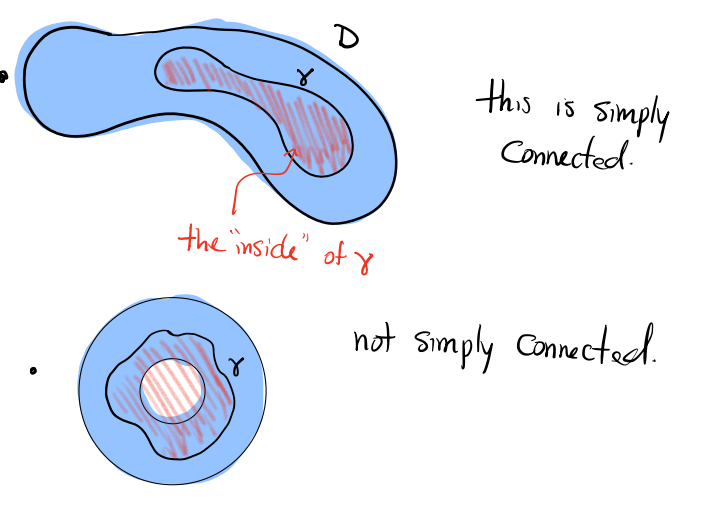
\includegraphics[width=0.5\textwidth]{LECTURE_7/simply-connected.png}
    \caption{Simply Connected Domain}
\end{figure}

\begin{theorem}
    [Cauchy's Theorem]
    Suppose $f$ is analytic on a domain $D$, and let $\gamma$ be a $C^1$ simple closed curve in $D$ such that the inside of $\gamma = \Omega \subset D$. Then:
    $$\oint_{\gamma} f(z) dz = 0$$
\end{theorem}

\begin{proof}
    By Green's Theorem:
    $$\oint_{\gamma} f(z) dz = i\iint_{\Omega} \left(\frac{\partial f}{\partial x} - \frac{\partial f}{\partial y}\right) dxdy$$
    But if $f = u + iv$ is analytic, so:
    \begin{align*}
        \frac{\partial f}{\partial x} & = \frac{\partial u}{\partial x} + i \frac{\partial v}{\partial x}                 \\
                                      & = \frac{\partial v}{\partial y} - i \frac{\partial u}{\partial y}                 \\
                                      & = -i \left(\frac{\partial u}{\partial y} + i \frac{\partial v}{\partial y}\right) \\
                                      & = -i \frac{\partial f}{\partial y}
    \end{align*}
    So $\frac{\partial f}{\partial x} + i \frac{\partial f}{\partial y} = 0$ and the result follows.
\end{proof}

\begin{theorem}
    [More General Cauchy's Theorem]
    if $D$ is a simply connected domain and $\gamma$ is any closed, piecewise $C^1$ curve in $D$, then, if $f$ is analytic on $D$:
    $$\oint_{\gamma} f(z) dz = 0$$
    \begin{figure}[H]
        \centering
        \begin{subfigure}{0.5\textwidth}
            \centering
            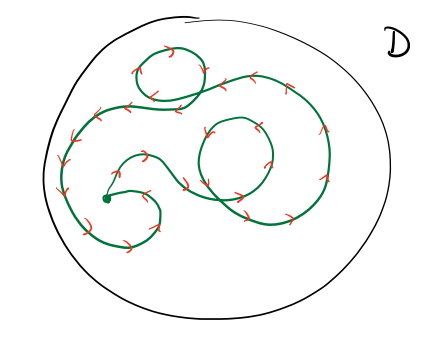
\includegraphics[width=0.5\textwidth]{LECTURE_7/1.png}
            \caption{Simply Connected Domain in $D$}
        \end{subfigure}
        \begin{subfigure}{0.5\textwidth}
            \centering
            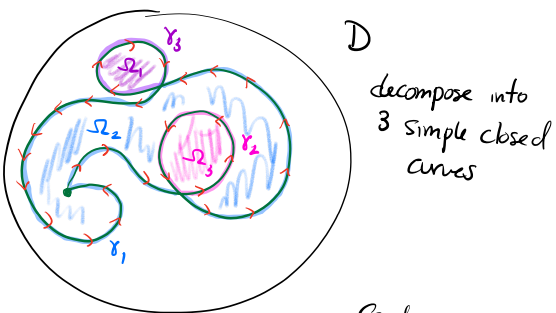
\includegraphics[width=0.5\textwidth]{LECTURE_7/2.png}
            \caption{Decomposition of $\gamma$}
        \end{subfigure}
    \end{figure}
    $$ \oint_{\gamma} f(z) dz = \oint_{\gamma_1} f(z) dz + \oint_{\gamma_2} f(z) dz +  \oint_{\gamma_3} f(z) dz = 0$$
\end{theorem}

\begin{theorem}
    [Differentiability of Analytic Functions]
    If $D$ is a simply connected domain and f is analytic on $D$, then there is an analytic function $F$ on $D$ such that $F^\prime = f$.
\end{theorem}
\begin{lemma}
    For $F(z) = \int_{\gamma}f(z)dz$, $F$ is independent of the path $\gamma$.
\end{lemma}
\begin{proof}
    Let's say $\gamma_1$ and $\gamma_2$ are two paths from $z_0$ to $z_1$, and $\Gamma = \gamma_1 - \gamma_2$. Then:
    \begin{align*}
        \oint_{\Gamma} f(z) dz & = \oint_{\gamma_1} f(z) dz - \oint_{\gamma_2} f(z) dz \\
        0                      & = F_1 - F_2                                           \\
        F_1                    & = F_2
    \end{align*}
    \begin{figure}[H]
        \centering
        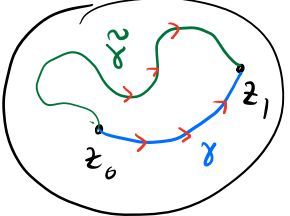
\includegraphics[width=0.5\textwidth]{LECTURE_7/independent.png}
    \end{figure}
\end{proof}
\begin{theorem}
    [Cauchy's Integral Formula]
    Suppose $f$ is analytic on a domain $D$, $\gamma$ is piecewise $C^1$, positively oriented, simple closed curve in $D$ such that: $\text{inside}( \gamma) = \Omega \subset D$. Then:
    $$f(z_0) = \frac{1}{2\pi i} \oint_{\gamma} \frac{f(\xi)}{\xi - z} d\xi\qquad \forall z \in \Omega$$
\end{theorem}

\begin{proof}
    \begin{figure}[H]
        \centering
        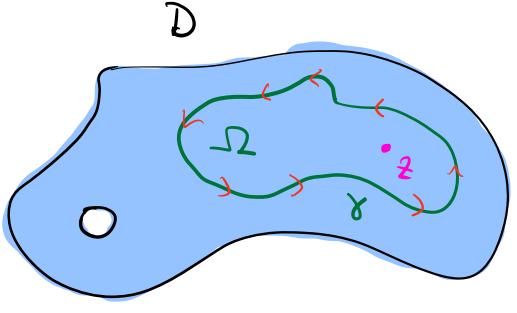
\includegraphics[width=0.5\textwidth]{LECTURE_7/cauchy-integral.png}
    \end{figure}
    Let $g(\xi) = \frac{f(\xi)}{\xi - z}$ be an analytic function in $\Omega/\{z\}$.\\
    Let $D_{\epsilon}(z) = \{z \in \mathbb{C} | |z - z_0| < \epsilon\}$ be a disc of radius $\epsilon$ centered at $z_0$.\\
    We choose $\epsilon$ to be small such that $D_{\epsilon}(z) \subset \Omega$.\\
    By Cauchy's Theorem:
    \begin{align*}
        \oint_{\gamma} \frac{f(\xi)}{\xi - z} d\xi & = \oint_{\partial D_{\epsilon}(z)} \frac{f(\xi)}{\xi - z} d\xi
    \end{align*}
    \textit{Note: $\partial D_{\epsilon}(z)$ is the boundary of $D_{\epsilon}(z)$}.\\
    Now we parametrize $\partial D_{\epsilon}(z)$ by $\partial D_{\epsilon} = z + \epsilon e^{i\theta}$, $0 \leq \theta \leq 2\pi$, Then:
    \begin{align*}
        \oint_{\partial D_{\epsilon}(z)} \frac{f(\xi)}{\xi - z} d\xi & = \int_{0}^{2\pi} \frac{f(z + \epsilon e^{i\theta})}{\epsilon e^{i\theta}} \epsilon i e^{i\theta} d\theta \\
                                                                     & = i \int_{0}^{2\pi} f(z + \epsilon e^{i\theta}) d\theta
    \end{align*}
    as $\epsilon \to 0$, $f(z + \epsilon e^{i\theta}) \to f(z)$ (by continuity of $f$).\\
    Hence:
    \begin{align*}
        \lim_{\epsilon \to 0} i \int_{0}^{2\pi} f(z + \epsilon e^{i\theta}) d\theta & = 2\pi i f(z) \\
    \end{align*}
    Thus
    $$\boxed{\oint_{\gamma} \frac{f(\xi)}{\xi - z} d\xi = 2\pi i f(z)}$$
\end{proof}

\section{Applications of Cauchy's Integral Formula}

\begin{example}
    Compute:
    $$\int_{0}^{2\pi} \frac{d\theta}{2 + \sin \theta}$$

    \hrule
    \vspace{1em}
    \textbf{\underline{Idea:}} Write this as an integral for an analytic function over the circle $z = e^{i\theta} \quad 0 \leq \theta \leq 2\pi$. \\
    If $|z| = 1$, then
    \begin{align*}
        \sin \theta        & = \frac{e^{i\theta} - e^{-i\theta}}{2i} \\
                           & = \frac{z - z^{-1}}{2i}                 \\ \\
        \therefore d\theta & = \frac{dz}{iz}
    \end{align*}
    So, integral is:
    \begin{align*}
        \int_{\gamma(\theta) = e^{i\theta}} \frac{1}{2 + \frac{z - z^{-1}}{2i}} \frac{dz}{iz} & = \int_{\gamma} \frac{2dz}{4iz + (z^2 - 1)}                                                                                \\
        \rightarrow z^2 - 4iz - 1                                                             & = \left[z - \left(\frac{-4i + \sqrt{-16 + 4}}{2}\right)\right]\left[z - \left(\frac{-4i - \sqrt{-16 + 4}}{2}\right)\right] \\
                                                                                              & = (z - i(\sqrt{3}-2))(z + (\sqrt{3} + 2)i)
    \end{align*}
    Since $|\sqrt{3} - 2| < 1, |\sqrt{3} + 2| > 1$, we can apply the cauchy integral formula:
    \begin{figure}[H]
        \centering
        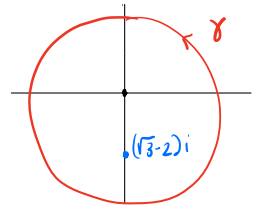
\includegraphics[width=0.5\textwidth]{LECTURE_7/example.png}
        \caption{Circle of Radius 1}
    \end{figure}
    \begin{align*}
        \int_{\gamma} \frac{1}{(z - i(\sqrt{3} - 2))}\cdot \frac{2dz}{(z + i(\sqrt{3} + 2))} & = 2\pi i \left(\frac{2}{(\sqrt(3)-2)i + (\sqrt{3} + 2)i}\right) \\
                                                                                             & = \frac{4\pi}{2\sqrt{3}}                                        \\
                                                                                             & = \frac{2\pi}{\sqrt{3}}
    \end{align*}
\end{example}

\chapter{Homework 3}

\begin{example}
    [Fisher, Section 2.2, Problem 2]

    Find the radius of convergence for the series

    $$\sum_{k=0}^\infty\frac{(k!)^2}{(2k)!}(z-2)^k$$

    \hrule
    \vspace{0.5cm}

    Let $a_k = \frac{(k!)^2}{(2k)!}$, then

    \begin{align*}
        \lim_{k\to\infty}\left|\frac{a_{k+1}}{a_k}\right| & = \lim_{k\to\infty}\left|\frac{(k+1)!^2}{(2k+2)!}\cdot\frac{(2k)!}{(k!)^2}\right| \\
                                                          & = \lim_{k\to\infty}\left|\frac{(k+1)^2}{(2k+2)(2k+1)}\right|                      \\
                                                          & = \lim_{k\to\infty}\left|\frac{k^2+2k+1}{4k^2+6k+2}\right|                        \\
                                                          & = \lim_{k\to\infty}\left|\frac{1+2/k+1/k^2}{4+6/k+2/k^2}\right|                   \\
                                                          & = \left|\frac{1}{4}\right| = \frac{1}{4}
    \end{align*}

    Therefore, the radius of convergence is $R = \frac{1}{1/4} = 4$.

\end{example}


\begin{example}
    [Fisher, Section 2.2, Problem 4]

    Find the radius of convergence for the series

    $$\sum_{k=0}^\infty(-1)^kz^{2k}$$

    \hrule
    \vspace{0.5cm}

    We can relate this to a geometric series with $a = 1$ and $r = -z^2$. The limit of the ratio of consecutive terms is
    \begin{align*}
        L = \frac{1}{1 - (-z^2)} = \frac{1}{1 + z^2}
    \end{align*}

    Provided that $|r| = |-z^2| < 1$. Therefore, the radius of convergence is $R = 1$.

\end{example}


\begin{example}
    [Fisher, Section 2.2, Problem 22]

    (a) If $f(z)=\sum_{n=0}^\infty a_n(z-z_0)^n$ has radius of convergence $R>0$,and if $f(z)=0$ for all $z$ such that $|z-z_0|<r\leq R$, show that all the coefficients are zero (ie. $a_0=a_1=a_2=\cdots=0).$
    \\
    (b) if $F(z)=\sum_{n=0}^\infty a_n(z-z_0)^n$ and $G(z)=\sum_{n=0}^\infty b_n(z-z_0)^n$ are convergent and equal on some disc $|z-z_0|<r$,show that

    $a_n=b_n$ for all $n.$

    \hrule
    \vspace{0.5cm}

    (a)     if $f(z)$ is analytic in a domain $D, z_0 \in D$ and $\{|z-z_0| < R\} \subseteq D$, then $f(z)$ hasa convergent power series expansion about $z_0$ given by:
    \begin{equation}
        f(z) = \sum_{n=0}^{\infty} a_n(z-z_0)^n
    \end{equation}
    Where:
    \begin{equation}
        a_n = \frac{1}{2\pi i} \int_{\gamma} \frac{f(z)}{(z-z_0)^{n+1}} dz
    \end{equation}
    for any simple, closed, positively oriented curve $\gamma$ in $D$ containing $z_0$ and $\gamma=|z-z_0| = R$.\\
    This means that functions that are equal on a disc of radius $r$ must have the same power series expansion. Furthermore, $a_n = 0$ being a valid power series expansion for $f(z)$ means it's the only power series expansion for $f(z)$.

    (b) If $F(z) = G(z)$ on a disc of radius $r$, using the previous theorem, $F(z)$ and $G(z)$ must have the same power series expansion. Therefore, $a_n = b_n$ for all $n$.
\end{example}

\begin{example}
    (Fisher, Section 2.3, Problem 2) Evaluate the following integral:

    $$\int_{|z|=2}\frac{e^z}{z(z-3)}dz$$

    \hrule
    \vspace{0.5cm}

    We can use Cauchy's Integral Formula to evaluate this integral. Let $f(z) = \frac{e^z}{z-3}$ and $z_0 = 0$. Then, the integral evaluates to:

    \begin{align*}
        \int_{|z|=2}\frac{e^z}{z(z-3)}dz & = 2\pi i f(0) = 2\pi i \frac{e^0}{-3} = -\frac{2\pi i}{3}
    \end{align*}
\end{example}

\begin{example}
    [Fisher, Section 2.3, Problem 4]
    Evaluate the following integral:
    $$\int_{|z|=1}\frac{\sin(z)}zdz$$

    \hrule
    \vspace{0.5cm}

    We can use Cauchy's Integral Formula to evaluate this integral. Let $f(z) = \sin(z)$ and $z_0 = 0$. Then, the integral evaluates to:
    \begin{align*}
        \int_{|z|=1}\frac{\sin(z)}zdz & = 2\pi i f(0) = 2\pi i \sin(0) = 0
    \end{align*}
\end{example}

\begin{example}
    [Fisher, Section 2.3, Problem 8]

    Evaluate the following definite trigonometric integral. (Hint: it may be useful to review the technique of Examples 6 and 7 of Section

    2.3).

    $$\int_0^\pi\frac1{1+\sin^2\theta}d\theta $$

    \hrule
    \vspace{0.5cm}

    We know that:
    \begin{align*}
        \sin\theta = \frac{e^{i\theta} - e^{-i\theta}}{2i}
    \end{align*}
    So we can parametrize using the relation, $z = e^{i\theta}$:
    \begin{align*}
        \sin^2\theta & = \frac{e^{i\theta} - e^{-i\theta}}{2i} \cdot \frac{e^{i\theta} - e^{-i\theta}}{2i} \\
                     & = \frac{(e^{i\theta})^2 - 2 + (e^{i\theta})^-2}{-4}                                 \\
                     & = \frac{z^2 - 2 + z^{-2}}{-4}
    \end{align*}
    And the differential becomes:
    \begin{align*}
        d\theta & = \frac{dz}{iz}
    \end{align*}
    So the integral becomes:
    \begin{align*}
        \int_0^\pi\frac1{1+\sin^2\theta}d\theta & = \int_{|z|=1}\frac{1}{1 + \frac{z^2 - 2 + z^{-2}}{-4}} \frac{dz}{iz} \\
                                                & = \int_{|z|=1}\frac{-4iz}{z^4 - 6z^2 + 1} dz
    \end{align*}

    We can find the roots using the quadratic formula ($z^2 = \frac{-b \pm \sqrt{b^2 - 4ac}}{2a}$ with $a = 1, b = -6, c = 1$)

    \begin{align*}
        z^2 & = \frac{-6 \pm \sqrt{36 - 4}}{2} = \frac{-6 \pm \sqrt{32}}{2} = 3 \pm 2\sqrt{2} \\
        z   & = \pm\sqrt{3 \pm 2\sqrt{2}}                                                     \\
    \end{align*}
    Now let's rewrite the integral in terms of $z$:
    \begin{align*}
         & \int_{|z|=1}\frac{-4iz}{z^4 - 6z^2 + 1} dz  =                                                                                        \\
         & \int_{|z|=1}\frac{-4iz}{(z - \sqrt{3 + 2\sqrt{2}})(z + \sqrt{3 + 2\sqrt{2}})(z - \sqrt{3 - 2\sqrt{2}})(z + \sqrt{3 - 2\sqrt{2}})} dz
    \end{align*}
    We choose $|(z - \sqrt{3 - 2\sqrt{2}})| < 1$ as the contour of integration and we can write:
    \begin{align*}
        f(z) = \frac{-4iz}{(z + \sqrt{3 - 2\sqrt{2}})(z - \sqrt{3 + 2\sqrt{2}})(z + \sqrt{3 + 2\sqrt{2}})}
    \end{align*}
    So the integral evaluates to:
    \begin{align*}
        \int_{|z|=1}\frac{-4iz}{z^4 - 6z^2 + 1} dz & = \int_{|z|=1}\frac{\frac{-4iz}{(z + \sqrt{3 - 2\sqrt{2}})(z - \sqrt{3 + 2\sqrt{2}})(z + \sqrt{3 + 2\sqrt{2}})}}{(z - \sqrt{3 - 2\sqrt{2}})} dz
    \end{align*}
    Applying Cauchy's Integral Formula, we get:
    \begin{align*}
         & \int_{|z|=1}\frac{-4iz}{z^4 - 6z^2 + 1} dz = 2\pi i f(\sqrt{3 - 2\sqrt{2}})                                                                            \\
         & = 2\pi i \frac{-4i\sqrt{3 - 2\sqrt{2}}}{2\sqrt{3 - 2\sqrt{2}}(\sqrt{3 - 2\sqrt{2}} - \sqrt{3 + 2\sqrt{2}})(\sqrt{3 - 2\sqrt{2}}+\sqrt{3 + 2\sqrt{2}})} \\
         & = 2\pi i (\frac{i}{2\sqrt2})                                                                                                                           \\
         & = -\frac{\pi}{\sqrt{2}}
    \end{align*}
\end{example}

\begin{example}
    [Fisher, Section 2.3, Problem 10]

    Evaluate the following integral.(Hint: It may be useful to review the technique of Example 10 of Section 2.3)
    $$\int_\gamma(z+z^{-1})dz$$


    Where $\gamma$ is any curve contained in the region $\{$Im$( z) > 0\}$ which joints $-4+i$ to $6+2i.$

    \hrule
    \vspace{0.5cm}

    We know that the derivative of $F(z) = \frac{z^2}{2} + \ln(z)$ is $f(z) = z + z^{-1}$. But this is valid only where $\ln(z)$ is analytic, which is the case for $\{$Im$( z) > 0\}$. So the integral evaluates to:
    \begin{align*}
        \int_\gamma(z+z^{-1})dz & = \int_\gamma f(z)dz = \int_\gamma F'(z)dz                        \\
                                & = F(\text{end}) - F(\text{start})                                 \\
                                & = F(6+2i) - F(-4+i)                                               \\
                                & = \frac{(6+2i)^2}{2} + \ln(6+2i) - \frac{(-4+i)^2}{2} - \ln(-4+i) \\
                                & = 8.5 + 16i + \ln(6 + 2i) - \ln(-4 + i)
    \end{align*}
\end{example}

\begin{example}
    [Fisher, Section 2.3, Problem 14]

    (a)(5 points) Suppose $f$ is analytic on the disc $|z-z_0|<R$.Show that for any $r<R$ we have

    $$f(z_0)=\frac1{2\pi}\int_0^{2\pi}f(z_0+re^{it})dt$$

    (b) (5 points) Using part (a) and the triangle inequality, conclude that

    $$|f(z_0)|\leq\max_{0\leq t\leq2\pi}|f(z_0+re^{it})|$$

    (c)(5 points) Conclude from (b) that $|f|$ cannot have a strict local maximum within the domain of analyticity of $f$

    \hrule
    \vspace{0.5cm}

    (a) The Cauchy Integral Formula states that for any $r<R$:
    \begin{align*}
        f(z_0) & = \frac{1}{2\pi i} \int_{|z-z_0| = r} \frac{f(z)}{z - z_0} dz
    \end{align*}
    We can parametrize the integral using:
    \begin{align*}
        z  & = z_0 + re^{it} \quad \text{where} \quad 0 \leq t \leq 2\pi \\
        dz & = ire^{it}dt
    \end{align*}
    So the integral becomes:
    \begin{align*}
        f(z_0) & = \frac{1}{2\pi i} \int_{0}^{2\pi} \frac{f(z_0 + re^{it})}{re^{it}} ire^{it} dt \\
               & = \frac{1}{2\pi} \int_{0}^{2\pi} f(z_0 + re^{it}) dt
    \end{align*}
    As required.
    (b) using what we found in part (a), we can write:
    \begin{align*}
        f(z_0) & = \frac{1}{2\pi} \int_{0}^{2\pi} f(z_0 + re^{it}) dt \\
    \end{align*}
    Thus:
    \begin{align*}
        \left|\frac{1}{2\pi} \int_{0}^{2\pi} f(z_0 + re^{it}) dt \right|         & \leq \frac{1}{2\pi} \int_{0}^{2\pi} |f(z_0 + re^{it})| dt                     \\
        \frac{1}{2\pi} \int_{0}^{2\pi} |f(z_0 + re^{it})| dt                     & \leq \frac{1}{2\pi} \int_{0}^{2\pi} \max_{0\leq t\leq2\pi}|f(z_0+re^{it})| dt \\
        \text{Since the maximum is constant}                                     & \text{, we can take it out of the integral}                                   \\
        \frac{1}{2\pi} \int_{0}^{2\pi} \max_{0\leq t\leq2\pi}|f(z_0+re^{it})| dt & =\max_{0\leq t\leq2\pi}|f(z_0+re^{it})| \frac{1}{2\pi}  \int_{0}^{2\pi} dt    \\
                                                                                 & = \max_{0\leq t\leq2\pi}|f(z_0+re^{it})|
    \end{align*}
    Therefore I can write:
    \begin{align*}
        |f(z_0)|\leq\max_{0\leq t\leq2\pi}|f(z_0+re^{it})|
    \end{align*}

    (c) If $|f|$ has a strict local maximum at $z_0$, then $|f(z_0)| > |f(z_0 + re^{it})|$ for some $r<R$. But this contradicts the inequality we found in part (b). Therefore, $|f|$ cannot have a strict local maximum within the domain of analyticity of $f$.
\end{example}

\chapter{Lecture 8: Consequences of Cauchy's Integral Formula}

\begin{theorem}
    if $f(z)$ is analytic in a domain $D, z_0 \in D$ and $\{|z-z_0| < R\} \subseteq D$, then $f(z)$ hasa convergent power series expansion about $z_0$ given by:
    \begin{equation}
        f(z) = \sum_{n=0}^{\infty} a_n(z-z_0)^n
    \end{equation}
    Where:
    \begin{equation}
        a_n = \frac{1}{2\pi i} \int_{\gamma} \frac{f(z)}{(z-z_0)^{n+1}} dz
    \end{equation}
    for any simple, closed, positively oriented curve $\gamma$ in $D$ containing $z_0$ and $\gamma=|z-z_0| = R$.
\end{theorem}

\begin{proof}
    Let $\Delta = \{|z-z_0| < R\}$. if $z \in \Delta$, $|z - z_0| = s < R$, then by Cauchy's Integral Formula:
    \begin{equation}
        f(z) = \frac{1}{2\pi i} \int_{\gamma} \frac{f(\zeta)}{\zeta - z} d\zeta
    \end{equation}
    Where $\gamma = \{|z - z_0| = r\}$, positively oriented, $r > s$.\\
    \begin{figure}[H]
        \centering
        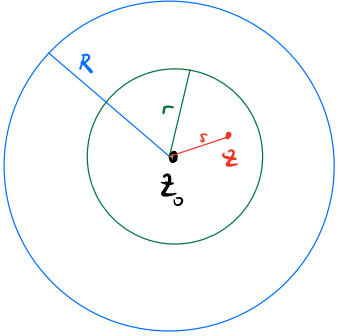
\includegraphics[scale=0.5]{LECTURE_8/proof.png}
    \end{figure}
    Now we write:
    \begin{align*}
        \xi - z & = \xi -z_0 - (z - z_0)                                   \\
                & = (\xi - z_0) \left(1 - \frac{z - z_0}{\xi - z_0}\right) \\
    \end{align*}
    Since $\frac{z - z_0}{\xi - z_0}  = \frac{s}{r} < 1$, we can write (for $\xi \in \gamma$):
    \begin{equation}
        \frac{1}{1 - \frac{z - z_0}{\xi - z_0}} = \sum_{k=0}^{\infty} \left(\frac{z - z_0}{\xi - z_0}\right)^k \qquad \text{Geometric Series}
    \end{equation}
    So, \textit{for any $N \in \mathbb{N}$ we have}:
    \begin{align*}
        f(z) & = \frac{1}{2\pi i} \int_{\gamma} \frac{f(\xi)}{\xi - z_0} \sum_{k=0}^{\infty} \left(\frac{z - z_0}{\xi - z_0}\right)^k d\xi                  \\
             & = \sum_{k=0}^{N} (z - z_0)^k \left(\frac{1}{2\pi i} \int_{\gamma} \frac{f(\xi)}{(\xi - z_0)^{k+1}} d\xi\right)                               \\
             & + \frac{1}{2\pi i} \int_{\gamma} \frac{f(\xi)}{\xi - z_0} \left[ \sum_{k=N+1}^{\infty} \left(\frac{z - z_0}{\xi - z_0}\right)^k \right] d\xi
    \end{align*}
    Since $\sum_{k=0}^{\infty} \frac{|z - z_0|^k}{|\xi - z_0|^k}$ converges, if $\epsilon > 0$\\
    We can choose $L$ such that $\forall N > L$ we have:
    \begin{equation}
        \sum_{k=N+1}^{\infty} \frac{|z - z_0|^k}{|\xi - z_0|^k} < \epsilon
    \end{equation}
    Since $f$ analytic, there is a constant $M$ such that $\max|f(\xi)| \leq M$ for $\xi \in \gamma$.\\
    By definition: $|\xi - z_0| = r$ on $\gamma$, thus, by the triangle inequality:
    \begin{align*}
        \frac{1}{2\pi i} \int_{\gamma} \frac{f(\xi)}{\xi - z_0} \left[ \sum_{k=N+1}^{\infty} \left(\frac{z - z_0}{\xi - z_0}\right)^k \right] d\xi \geq \frac{\text{length}(\gamma)}{r} M \epsilon = 2\pi M \epsilon
    \end{align*}
    Thus, $\forall \epsilon > 0, \exists L | \forall N > L$ we have:
    \begin{equation}
        \left| f(z) - \sum_{k=0}^{N} a_k(z - z_0)^k \right| < 2\pi \epsilon
    \end{equation}
    Where $a_k = \frac{1}{2\pi i} \int_{\gamma} \frac{f(\xi)}{(\xi - z_0)^{k+1}} d\xi$.
    So: $f(z) = \sum_{k=0}^{\infty} a_k(z - z_0)^k$. as desired.

\end{proof}
\begin{corollary}
    If $f(z)$ is analytic in a domain $D$, then so is $f'(z)$. In particular, if $f$ is analytic, then it is infinitely differentiable.
\end{corollary}

\begin{proof}
    Every $f$ has a power series expansion about $z_0$, and every term in the series is analytic. Therefore, the series converges to an analytic function.
\end{proof}

\begin{corollary}
    [Unique Analytic Continuation] If $f(z)$ is analytic in a domain $D$, and $f(z) = 0$ for all $z \in \Delta \subseteq D$, then $f(z) = 0$ for all $z \in D$.
    In the above setting we have:
    \begin{equation}
        \frac{f^{(k)}(z_0)}{k!} = \frac{1}{2\pi i} \int_{\gamma} \frac{f(\xi)}{(\xi - z_0)^{k+1}} d\xi
    \end{equation}
    In particular, if $f$ is analytic in a domain $D$, and, for some $z_0 \in D$, $f^{(k)}(z_0) = 0$ for all $k \in \mathbb{N}$, then $f(z) = 0 \forall z \in D$.
\end{corollary}
\section{Comparison with Real Functions}

\begin{example}
    To get a sense for the difference between real and complex functions, consider the following \textbf{real function}:
    \begin{equation}
        f(x) = \begin{cases}
            e^{-1/x^2} & x > 0    \\
            0          & x \leq 0
        \end{cases}
    \end{equation}
    $f$ is infinitely differentiable, and $\forall k \in \mathbb{N}$, $f^{(k)}(0) = 0$.\\
    So, the Taylor series of $f$ at $0 \in \mathbb{R}$ is:
    \begin{equation}
        f(x) = \sum_{k=0}^{\infty} \frac{f^{(k)}(0)}{k!} x^k = 0
    \end{equation}
    Thus, $f$ is infinitely differentiable, but \textbf{\underline{\textit{not}}} equal to a power series in any neighborhood of $0\in \mathbb{R}$.
\end{example}

\chapter{Lecture 9: More Applications of Cauchy's theorem}

\section{The order of a zero of a function}

\begin{lemma}
    [Order of a zero of a function]
    Suppose $f$ is analytic in a disc $D$, $f$ is not identically zero, and $f(z_0) = 0$. Then for some $z_0$ in $D$, we have
    \begin{equation*}
        f(z) = \sum_{n=0}^{\infty} a_n(z - z_0)^n
    \end{equation*}
    Let $m \geq 1$ be the smallest $n \in \mathbb{Z}_{\geq 0}$ such that $a_n \neq 0$. That is:
    \begin{equation*}
        f(z) = a_m(z - z_0)^m + a_{m+1}(z - z_0)^{m+1} + \cdots
    \end{equation*}
    \underline{Say:} $f$ has a zero of order $m$ at $z_0$.
    Equivalently:
    \begin{equation*}
        f(z) = f^{\prime}(z_0) = f^{\prime\prime}(z_0) = \cdots = f^{(m-1)}(z_0) = 0 \label{eq:order_of_zero}
    \end{equation*}
    Yet $f^{(m)}(z_0) \neq 0$. \\
    \underline{Then} $g(z) = \frac{f(z)}{(z - z_0)^m}$ is analytic in $D$ and $g(z_0) \neq 0$.
    \underline{Since}
    \begin{equation*}
        g(z) = a_m + a_{m+1}(z - z_0) + \cdots
    \end{equation*}
    Converges because:
    \begin{equation*}
        (z - z_0)^m \left[ a_{m+1} + a_{m+2}(z - z_0) + \cdots \right] = f(z) - a_m(z - z_0)^m
    \end{equation*}
    Converges in $D$.

\end{lemma}

\begin{proof}
    This proof will demonstrate the conclusion of equation \ref{eq:order_of_zero}. \\
    \underline{Let} $f(z) = a_m(z - z_0)^m + a_{m+1}(z - z_0)^{m+1} + \cdots$ \\
    Notice that $(z - z_0) = 0$ at $z = z_0$. \\
    \underline{Thus:}
    \begin{align*}
        f^{\prime}(z)       & = m a_m(z - z_0)^{m-1} + (m+1)a_{m+1}(z - z_0)^m + \cdots = 0           \\
        f^{\prime\prime}(z) & = m(m-1)a_m(z - z_0)^{m-2} + (m+1)m a_{m+1}(z - z_0)^{m-1} + \cdots = 0 \\
                            & \vdots                                                                  \\
        f^{(m-1)}(z)        & = m! a_m(z - z_0) + m! a_{m+1}(z - z_0)^2 + \cdots = 0                  \\
        f^{(m)}(z)          & = m! a_{m}(z - z_0)^0 + m! a_{m+1}(z - z_0)^1 + \cdots \neq 0
    \end{align*}
\end{proof}

\section{A partial converse to the Cauchy integral formula}
\begin{theorem}
    [Morera's Theorem]
    if $f$ is continuous in a domain $D$ and
    \begin{equation*}
        \int_{\gamma} f(z) \, dz = 0
    \end{equation*}
    for every triangle $\gamma$ where $\gamma \in D$, and inside$(\gamma) \subseteq D$, $f$ is analytic in $D$.
\end{theorem}
\begin{proof}
    \begin{align*}
        \Omega                   & = \{|z-z_0| < r\} \quad r > 0 \quad r\text{ is small} \\
        \text{such that } \Omega & \in D                                                 \\
        \text{for } z            & \in \ \Omega \quad \text{we define}                   \\
        F(z)                     & = \int_{\gamma} f(\zeta) \, d\zeta,
    \end{align*}
    where the integral is taken along a radial curve
    \begin{figure}[H]
        \centering
        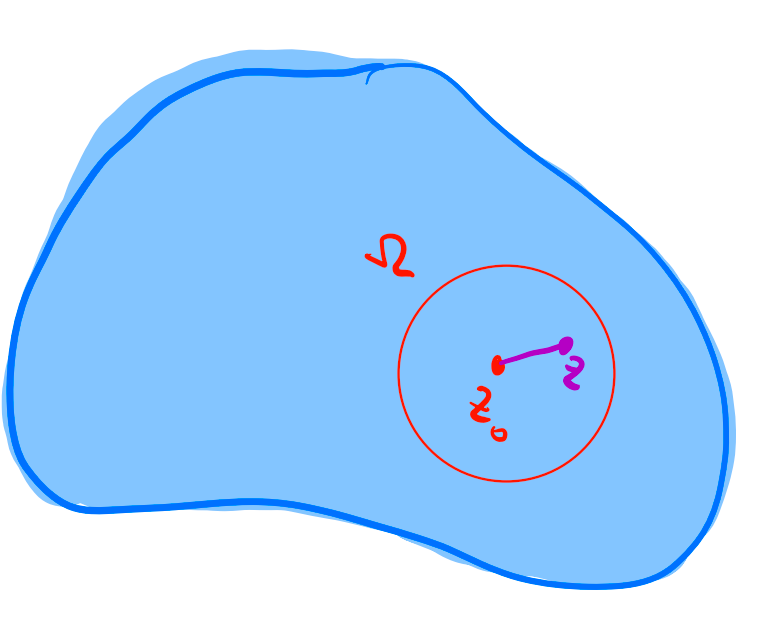
\includegraphics[width=0.4\textwidth]{./LECTURE_9/D.png}
        \caption{Radial curve}
        \label{fig:Radial curve}
    \end{figure}
    \textbf{\underline{Goal:}} F is analytic and F$^{\prime}(z) = f(z)$ (then it follows that $f$ is also analytic).
    \begin{equation*}
        F(z + h) - F(z) = \int_{z}^{z+h} f(\zeta) \, d\zeta
    \end{equation*}
    Since
    \begin{equation*}
        \int_{z_0}^{z} f(\zeta) \, d\zeta + \int_{z}^{z+h} f(\zeta) \, d\zeta - \int_{z_0}^{z+h} f(\zeta) \, d\zeta = 0
    \end{equation*}
    by assumption
    \begin{figure}[H]
        \centering
        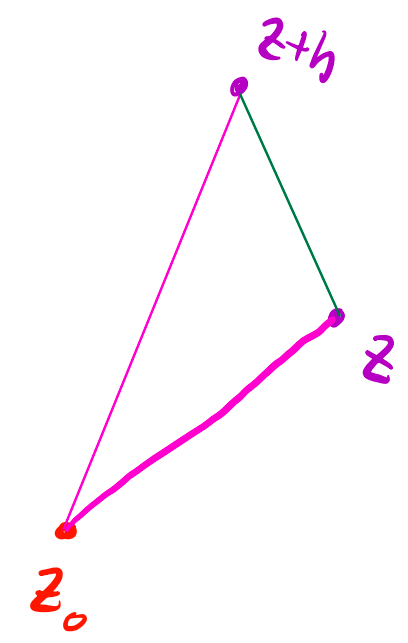
\includegraphics[width=0.4\textwidth]{./LECTURE_9/curve.png}
        \caption{Curve}
        \label{fig:Curve}
    \end{figure}
    \underline{\textbf{Thus:}}
    \begin{equation*}
        \frac{F(z+h) - F(z)}{h} - f(z) = \frac{1}{h} \int_{z}^{z+h} f(\zeta) - f(z)d\zeta
    \end{equation*}
    $\rightarrow$ This is because \begin{align*}
          & \int_{z}^{z+h} f(z)d\zeta \\
        = & f(z)\int_{z}^{z+h} d\zeta \\
        = & f(z) \cdot h
    \end{align*}
    By continuity of $f$, for any $\epsilon > 0$, there exists $\delta > 0$ such that $|f(w) - f(z)| < \epsilon$ if $|w - z| < \delta$.
    Then if $|h| < \delta$, we have:
    \begin{equation*}
        \left| \frac{F(z+h) - F(z)}{h} - f(z) \right| \leq \frac{1}{|h|} \epsilon |h| = \epsilon
    \end{equation*}
    Since $\epsilon$ is arbitrary, we have:
    \begin{equation*}
        \lim_{h \to 0} \frac{F(z+h) - F(z)}{h} = f(z)
    \end{equation*}
    \underline{\textbf{Thus:}} $F$ is analytic and $F^{\prime}(z) = f(z)$, as desired.
\end{proof}

\section{Applications}

\begin{theorem}
    [Liouville's Theorem]
    If $F$ is entire and $|F(z)| \leq M$ then $F$ is constant.
\end{theorem}

\begin{proof}
    \begin{align*}
        g(z)            & = \frac{F(z) - F(0)}{z} \quad \text{is entire since}                \\
        F(z)            & = F(0) + \sum_{n=1}^{\infty} a_n z^n                                \\
        \text{so } g(z) & = \sum_{n=1}^{\infty} a_n z^{n-1} = \sum_{n=0}^{\infty} a_{n+1} z^n
    \end{align*}
    Now
    \begin{equation*}
        |g(Re^{i\theta})| \leq \frac{|F(Re^{i\theta})| + |F(0)|}{R} \leq  \frac{2M}{R}
    \end{equation*}
    Using Cauchy's theorem, we have:
    \begin{align*}
        g(z_0) & = \frac{1}{2\pi} \int_{0}^{2\pi} \frac{g(z_0 + Re^{i\theta})}{Re^{i\theta}} \, iRe^{i\theta} \, d\theta \\
               & = \frac{1}{2\pi} \int_{0}^{2\pi} g(Re^{i\theta}) \, d\theta
    \end{align*}
    if $R >> |z_0|$, then $|z_0 + Re^{i\theta}| \geq R - |z_0|$
    \begin{figure}[H]
        \centering
        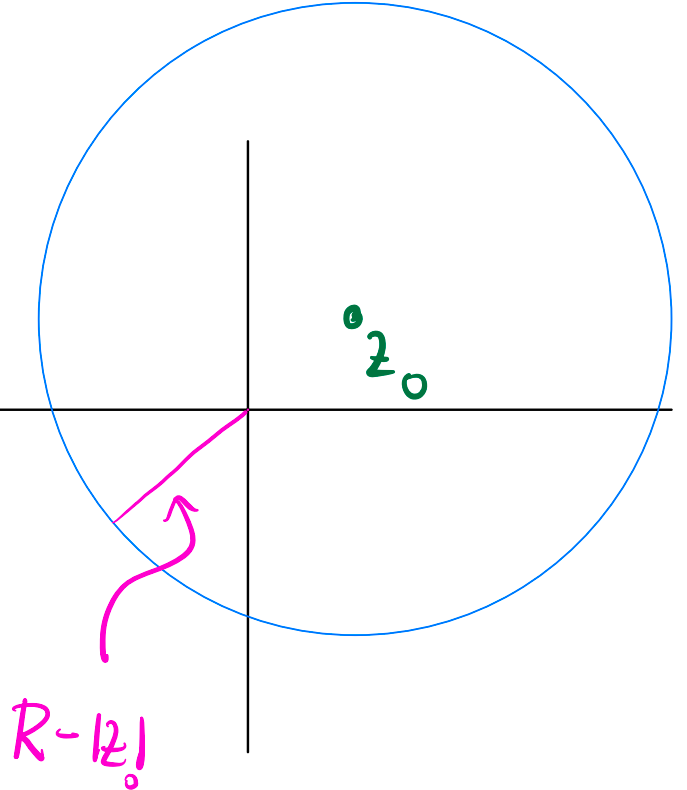
\includegraphics[width=0.4\textwidth]{./LECTURE_9/liouville.png}
        \caption{Circle}
        \label{fig:Circle}
    \end{figure}
    so
    \begin{equation*}
        |g(z_0)| \leq \frac{1}{2\pi} \int_0^{2\pi}|g(z_0 + Re^{i\theta})| \, d\theta \leq \frac{2M}{R-|z_0|}
    \end{equation*}
    But $R >> |z_0|$ is arbitrary, so taking $R \to \infty$ yields $g(z_0) = 0$ for all $z_0$ and $F(z_0) = F(0)$.
\end{proof}

\section{Analytic Logarithms}

\begin{lemma}
    [The logarithmic derivative]
    Let $D$ be a simply connected domain. \\
    Suppose $f$ is analytic in $D$ and $f \neq 0$ anywhere in $D$. \\
    Then $\frac{f^{\prime}}{f}$ is analytic in $D$ and hence so let's define:
    \begin{equation*}
        h^{\prime}(z) = \frac{f^{\prime}(z)}{f(z)}
    \end{equation*}
    Using the fundamental theorem of calculus, we have:
    \begin{equation*}
        h(z) = \int_{z_0}^{z} \frac{f^{\prime}(\zeta)}{f(\zeta)} \, d\zeta
    \end{equation*}
    Cauchy's theorem implies that $h(z)$ is analytic in $D$. \\
    Morera's theorem ensures that the integral can be taken over any path from $z_0$ to $z$ in $D$ and thus, $h(z)$ is path independent. \\
    So:
    \begin{align*}
        \left[e^{-h(z)}f(z)\right]^{\prime} & = -e^{-h(z)}h^{\prime}(z)f(z) + e^{-h(z)}f^{\prime}(z)              \\
                                            & = -e^{-h(z)}\frac{f^{\prime}(z)}{f(z)}f(z) + e^{-h(z)}f^{\prime}(z) \\
                                            & = 0
    \end{align*}
    So $e^{-h(z)}f(z) = f(z_0)$ is a constant. Or:
    \begin{align*}
        e^{-h(z)}f(z) & = f(z_0) \\
        f(z) = f(z_0)e^{h(z)}
    \end{align*}
    Thus $g (z) = h(z) + \text{Log}(f(z_0))$ satisfies:
    \begin{equation*}
        \begin{cases}
            e^{g(z)} = f(z) \\
            g(z) \quad \text{ is analytic in } D
        \end{cases}
    \end{equation*}
\end{lemma}

\section{Isolated Singularities}

\begin{definition}
    [Isolated Singularities]
    An analytic function has an \underline{isolated singularity at $z_0$} if it is analytic in a punctured disc $\{0 < |z - z_0| < r\}$ for some $r > 0$.
\end{definition}

\begin{example}
    $f(z) = \frac{z^2 - z_0^2}{z - z_0}$\\
    In this case $|f(z)|$ is bounded as $z \to z_0$. \\
    in fact, $f(z) = z + z_0$ ($z \neq z_0$) and $f$ can be extended to an analytic function at $z_0$.\\
    \underline{Thus:} $z_0$ is a \textbf{removable} singularity.
\end{example}

\begin{example}
    $f(z) = \frac{1}{(z - z_0)^4}$ \\

    $|f(z)| = \frac{1}{|z - z_0|^4} \to +\infty$ as $z \to z_0$.\\
    This is an example of a pole.
\end{example}

\begin{example}
    $f(z) = e^{\frac{1}{z - z_0}}$ \\

    $z_0 = 0$ for simplicity. \\
    $|f(z)| = e^{\frac{1}{2z} + \frac{1}{2\overline{z}}} = e^{\frac{x}{x^2 + y^2}}$ \\

    \begin{enumerate}
        \item If $y = 0$ and $x \to 0$ from $x > 0$, then $|f(z)| \to +\infty$.
        \item If $y = 0$ and $x \to 0$ from $x < 0$, then $|f(z)| \to 0$.
        \item If $x = 0$ and $y \to 0$ then $|f(z)| \to 1$, this is an \textbf{essential} singularity.
    \end{enumerate}
\end{example}

\section{Removable Singularities}

\begin{example}
    [Removable Singularity]
    Suppose $|f(z)|$ is bounded near $z_0$. \\
    Let
    \begin{equation*}
        g(z) = \begin{cases}
            (z-z_0)^2 f(z) & z \neq z_0 \\
            0              & z = z_0
        \end{cases}
    \end{equation*}
    \underline{Then}, $g(z)$ is analytic on $\{|z-z_0| < r\}$ for some $r > 0$. \\

    \underline{Since}\\
    \begin{equation*}
        \frac{g(z) - g(z_0)}{z - z_0} = (z - z_0)f(z)
    \end{equation*}
    \underline{and}
    \begin{equation*}
        \lim_{z \to z_0} (z - z_0)f(z) = 0
    \end{equation*}
    so $g'(z_0) = 0$ and thus:
    \begin{equation*}
        g(z)  = a_2(z-z_0)^2 + a_3(z-z_0)^3 + \cdots
    \end{equation*}
    \underline{So:}
    \begin{equation*}
        f(z) = \frac{g(z)}{(z-z_0)^2} = a_2 + a_3(z-z_0) + \cdots
    \end{equation*}
    If we set $f(z_0) = a_2$, then $f$ is analytic on $\{|z - z_0| < r\}$ and, we have \underline{\textbf{removed}} the singularity.
\end{example}

\begin{definition}
    $z_0$ is a \underline{removable singularity} of $f$ is bounded in a neighborhood of $z_0$.
\end{definition}

\section{Poles}

\begin{remark}
    Recall: if $f$ is analytic on $\{0 < |z - z_0| < R \}$ and $\lim_{z \to z_0} f(z) = \infty$, then $z_0$ is a pole of $f$.
\end{remark}

\begin{lemma}
    [Poles]
    Choose $r < R$ small enough that $|f(z)| > 1$ on $\{0 < |z-z_0| < r \}$. \\
    \underline{Then}: $g(z) = \frac{1}{f(z)}$ is analytic on $\{0 < |z - z_0| < r\}$ and $g(z) \to 0$ as $z \to z_0$. \\
    Thus, $g$ has a removable singularity and $g(z_0) = 0$.\\
    $z_0$ is a zero of order $m \geq 1$
    \begin{equation*}
        g(z) = (z - z_0)^m h(z)
    \end{equation*}
    where $h(z)$ is analytic and $h(z_0) \neq 0$ on $\{|z - z_0| < r\}$. \\
    \underline{Then}
    \begin{equation*}
        f(z) = \frac{1}{g(z)} = \frac{1}{(z - z_0)^m} \cdot \frac{1}{h(z)} = \frac{H(z)}{(z - z_0)^m}
    \end{equation*}
    Where $H(z)$ is analytic on $\{|z-z_0| < r\}$ and $H(z_0) \neq 0$.
\end{lemma}

\begin{definition}
    if $f(z) = \frac{H(z)}{(z - z_0)^m}$, where $H(z)$ is analytic on $\{|z - z_0| < r\}$ and $H(z_0) \neq 0$, then we say $f(z)$ has a pole of order $m$ at $z_0$.
\end{definition}

\section{Essential Singularities}

\begin{remark}
    Recall $f(z) = e^{\frac{1}{z}}$ has an essential singularity at $z = 0$. The behaviour near essential singularities is wild.
\end{remark}

\begin{proposition}
    if $f$ is analytic on $\{0 < |z - z_0| < r\}$, with an essential singularity at $z_0$, then for any $w \in \mathbb{C}$, and any $\delta > 0, \exists z_\delta$ such that $0 < |z - z_0|< r$ and $|f(z) - w| < \delta$.
\end{proposition}


\chapter{Homework 4}

\begin{example}
    [Fisher, Section 2.4, Problem 10]

    find the power series expansion of $f(z) = e^z$ about the point $z_0 = \pi i$. What is the largest disc on which this series is valid?

    \hrule
    \vspace{0.5cm}

    We know that a taylor series is given by

    \begin{equation}
        f(z) = \sum_{n=0}^{\infty} \frac{f^{(n)}(z_0)}{n!} (z - z_0)^n
    \end{equation}
    for $f(z) = e^z$, we know that $f^{(n)}(z) = e^z$ for all $n \in \mathbb{N}$. Therefore, the taylor series expansion of $f(z)$ about $z_0 = \pi i$ is

    \begin{equation}
        e^z = \sum_{n=0}^{\infty} \frac{e^{\pi i}}{n!} (z - \pi i)^n
    \end{equation}

    The largest disk on which this series is valid can be found by using the ratio test. The ratio test states that a series converges if the limit of the ratio of the $(n+1)$th term to the $n$th term is less than 1. That is

    \begin{equation}
        \lim_{n \to \infty} \left| \frac{a_{n+1}}{a_n} \right| < 1
    \end{equation}

    for the series $\sum a_n$. In this case, we have

    \begin{equation}
        \lim_{n \to \infty} \left| \frac{e^{\pi i}}{(n+1)!} (z - \pi i)^{n+1} \cdot \frac{n!}{e^{\pi i}} (z - \pi i)^n \right|
    \end{equation}

    Simplifying, we get

    \begin{equation}
        \lim_{n \to \infty} \left| \frac{z - \pi i}{n+1} \right| = 0
    \end{equation}

    Therefore, $R = \frac{1}{L} = \infty$. This means that the series converges for all $z \in \mathbb{C}$.

\end{example}

\begin{example}
    [Fisher, Section 2.4, Problem 12]
    Find the power series expansion of $f(z) = \frac{z^2}{1-z}$ about $z_0 = 0$. What is the largest disc on which this series is valid?

    \hrule
    \vspace{0.5cm}

    We know that $\frac{1}{1-z}$ has a taylor series expansion about $z_0 = 0$ given by
    \begin{align*}
        \frac{1}{1-z} & = \sum_{n=0}^{\infty} z^n
    \end{align*}
    So, the taylor series expansion of $f(z)$ about $z_0 = 0$ is
    \begin{align*}
        f(z) & = z^2 \sum_{n=0}^{\infty} z^n \\
             & = \sum_{n=0}^{\infty} z^{n+2}
             & = \sum_{n=2}^{\infty} z^n
    \end{align*}

    The radius of convergence of this series is inherited from the radius of convergence of the series for $\frac{1}{1-z}$, which is $R = 1$.
\end{example}

\begin{example}
    [Fisher, Section 2.4, Problem 18]

    Using the (consequence of) the Cauchy Integral Formula, prove the Cauchy estimates:
    \[
        \left| f^{(n)}(z_0) \right| \leq \frac{n!}{r^n} \max_{\{|z - z_0| = r\}} |f(z)|, \quad n = 0, 1, 2, \dots,
    \]
    whenever \( f \) is analytic on a domain containing the set \( \{ |z - z_0| < r \} \).

    \hrule
    \vspace{0.5cm}

    If $f(z)$ is analytic on a domain containing the set $\{|z - z_0| < r\}$, then there exists a power series expansion of $f(z)$ about $z_0$ given by
    \begin{equation}
        f(z) = \sum_{n=0}^{\infty} a_n (z - z_0)^n
    \end{equation}

    We know that the \(n\)th derivative of \(f(z)\) is given by

    \begin{align*}
        f^{(n)}(z)   & = \sum_{k=n}^{\infty} a_k \frac{k!}{(k-n)!} (z - z_0)^{k-n} \\
        f^{(n)}(z_0) & = a_n n!
    \end{align*}

    The coefficient \(a_n\) are given by the following line integral where $\gamma$ is a simple, closed, positively oriented curve in $\{|z - z_0| < r\}$:

    \begin{align*}
        a_n            & = \frac{1}{2\pi i}\int_{\gamma} \frac{f(z)}{(z - z_0)^{n+1}} dz                                          \\
        a_n n!         & = \frac{n!}{2\pi i}\int_{\gamma} \frac{f(z)}{(z - z_0)^{n+1}} dz                                         \\
                       & \leq \frac{n!}{2\pi} \max_{\{|z - z_0| = r\}} \left|\int_{\gamma} \frac{f(z)}{(z - z_0)^{n+1}} dz\right| \\
                       & \leq \frac{n!}{2\pi} 2\pi r\max_{\{|z - z_0| = r\}} |\frac{f(z)}{r^{n+1}}|                               \\
                       & \leq n! \max_{\{|z - z_0| = r\}} \frac{|f(z)|}{r^{n}}                                                    \\
        |f^{(n)}(z_0)| & \leq \frac{n!}{r^{n}} \max_{\{|z - z_0| = r\}} |f(z)|
    \end{align*}

    As required.
\end{example}

\begin{example}
    [Fisher, Section 2.4, Problem 20]

    Suppose that $f(z)$ is an entire function and $\Re f(z) \leq c$ for all $z$. Show that $f$ is constant. (Hint: Consider $e^{f(z)}$.)

    \hrule
    \vspace{0.5cm}

    if $f(z)$ is an entire function, and $\Re f(z) \leq c$ for all $z$, then:
    \begin{align*}
        \Re f(z)     & \leq c                \\
        e^{\Re f(z)} & \leq e^c              \\
        g(z)         & = |e^{f(z)}| \leq e^c
    \end{align*}
    So by Liouville's theorem, $g(z) = C$ is constant and by extension:
    \begin{align*}
        e^{f(z)} & = C      \\
        f(z)     & = \log C
    \end{align*}
    $f(z)$ is also constant.
\end{example}

\begin{example}
    [Fisher, Section 2.4, Problem 21]
    Suppose that \( f(z) \) is an entire function and that there are constants \( A \), \( R_0 > 0 \) and \( m \in \mathbb{Z}_{>0} \) so that
    \[
        |f(z)| \leq A |z|^m \quad \text{for all } |z| \geq R_0.
    \]
    Show that \( f \) is a polynomial of degree at most \( m \). (Hint: Use Problem 3, above, for \( n > m \), and let \( r \to \infty \).)

    \hrule
    \vspace{0.5cm}

    The cauchy estimates state that for an entire function \( f(z) \) with a power series expansion about \( z_0 \) given by
    \[
        f(z) = \sum_{n=0}^{\infty} a_n (z - z_0)^n
    \]

    we have, for $z_0 = 0$:

    \begin{align*}
        |f^{(n)}(z_0)| & \leq \frac{n!}{r^n} \max_{\{|z - z_0| = r\}} |f(z)| \\
        |f^{(n)}(z_0)| & \leq \frac{n!}{r^n} \max_{\{|z| = r\}} A|z|^m       \\
        |f^{(n)}(z_0)| & \leq n! A r^{m-n}
    \end{align*}

    If \( f(z) \) is an entire function, then it must be defined for $r \to \infty$.

    \begin{align*}
        \lim_{r \to \infty} |f^{(n)}(z_0)| & \leq \lim_{r \to \infty} n! A r^{m-n} = \begin{cases}
                                                                                         0      & \text{if } n > m \\
                                                                                         n!A    & \text{if } n = m \\
                                                                                         \infty & \text{if } n < m
                                                                                     \end{cases}
    \end{align*}

    Because the limit of the $n^{th}$ derivative of \(f(z)\) as \(r \to \infty\) is 0 for \(n > m\), this implies that the power series expansion of \(f(z)\) is a polynomial of degree at most \(m\).
\end{example}

\begin{example}
    [Fisher, Section 2.4, Problem 22]

    Let \( D \) be a simply connected domain and \( f \) an analytic function on \( D \) that has no zeroes in \( D \). Let \( \gamma \neq 0 \) be a non-zero complex number. Show that there is an analytic function \( g \) on \( D \) such that \( f = g^{\gamma} \).

    \hrule
    \vspace{0.5cm}

    \begin{align*}
        f(z)                     & = g^{\gamma}                   \\
        \log f(z)                & = \gamma \log g                \\
        \frac{\log f(z)}{\gamma} & = \log g                       \\
        g(z)                     & = e^{\frac{\log f(z)}{\gamma}}
    \end{align*}
    Because $f(z)$ has no zeroes in $D$, we can define a branch of the logarithm, $\log f(z)$, such that it is analytic in $D$. And since $\gamma \neq 0$, $\frac{\log f(z)}{\gamma}$ is also analytic in $D$. Therefore, $g(z)$ is analytic in $D$.
\end{example}

\begin{example}
    [Fisher, Section 2.4, Problem 23]

    Locate the isolated singularities of \( f(z) = \frac{z^2}{\sin(z)} \). Identify each singularity as a removable singularity, a pole, or an essential singularity. If the singularity is removable, give the value of the function at the point.

    \hrule
    \vspace{0.5cm}

    We know $\sin(z)$ has zeros at $z = n\pi$ for $n \in \mathbb{Z}$. Therefore, $f(z)$ has singularities at $z = n\pi$ for $n \in \mathbb{Z}$. Near $z = n\pi$, $\sin(n \pi) \approx (-1)^n(z - n\pi)$. We can classify these singularities by examining the limit of $f(z)$ as $z \to n\pi$.

    \begin{align*}
        f(z) & = \frac{z^2}{\sin(z)}          \\
             & = \frac{z^2}{(-1)^n(z - n\pi)} \\
             & = \frac{z^2}{(-1)^n(z - n\pi)} \\
    \end{align*}
    at $z = 0$, $f(z)$ has a removable singularity, because
    \begin{align*}
        f(z) & = \frac{z^2}{(-1)^n(z - n\pi)} \\
             & = \frac{z^2}{(-1)^0(z - 0)}    \\
             & = z
    \end{align*}
    at $z = n\pi$, $f(z)$ has a pole of order 1, because
    \begin{align*}
        f(z) & = \frac{z^2}{(-1)^n(z - n\pi)} \\
             & = \frac{z^2}{(-1)^n(z - n\pi)} \\
    \end{align*}
\end{example}

\begin{example}
    [Fisher, Section 2.5, Problem 4]
    Locate the isolated singularities of \( f(z) = \pi \cot(\pi z) \). Identify each singularity as a removable singularity, a pole, or an essential singularity. If the singularity is removable, give the value of the function at the point.

    \hrule
    \vspace{0.5cm}

    \begin{align*}
        f(z) & = \pi \cot(\pi z)                     \\
             & = \pi \frac{\cos(\pi z)}{\sin(\pi z)} \\
             & \approx \pi \frac{(-1)^n}{\pi(z - n)} \\
    \end{align*}
    The above approximation is valid near $z = n$ for $n \in \mathbb{Z}$. We can classify these singularities by examining the limit of $f(z)$ as $z \to n$.

    \begin{align*}
        f(z)                & = \pi \frac{(-1)^n}{\pi(z - n)}                               \\
                            & = \frac{(-1)^n}{z - n}                                        \\
        \lim_{z \to n} f(z) & = \frac{(-1)^n}{0} = \infty \quad \text{On both sides of $n$}
    \end{align*}
    Therefore, $f(z)$ has poles of order 1 at $z = n$ for $n \in \mathbb{Z}$.
\end{example}

\begin{example}
    [Fisher, Section 2.5, Problem 6]

    Locate the isolated singularities of \( f(z) = \frac{e^z - 1}{e^{2z} - 1} \). Identify each singularity as a removable singularity, a pole, or an essential singularity. If the singularity is removable, give the value of the function at the point.

    \hrule
    \vspace{0.5cm}

    We can start by finding the zeros of the denominator, $e^{2z} - 1 = 0$:

    \begin{align*}
        e^{2z} - 1 & = 0                                           \\
        e^{2z}     & = 1                                           \\
        2z         & = 2\pi i n \quad \text{for } n \in \mathbb{Z} \\
        z          & = \pi i n \quad \text{for } n \in \mathbb{Z}
    \end{align*}

    To examine the singularities of $f(z)$, we can simplify the function:
    \begin{align*}
        f(z)   & = \frac{e^z - 1}{e^{2z} - 1}         \\
               & = \frac{e^z - 1}{(e^z - 1)(e^z + 1)} \\
               & = \frac{1}{e^z + 1}                  \\
        f(z_0) & = \frac{1}{e^{z_0} + 1}              \\
               & = \frac{1}{e^{\pi i n} + 1}          \\
               & = \frac{1}{1 + 1} = \frac{1}{2}
    \end{align*}
    Therefore, $f(z)$ has removable singularities at $z = \pi i n$ for $n \in \mathbb{Z}$ equal to $\frac{1}{2}$.
\end{example}

\begin{example}
    [Fisher, Section 2.5, Problem 16]

    Suppose \( f \) and \( g \) are analytic in \( |z - z_0| < R \) and \( f \) has a zero of order \( m \geq 1 \) at \( z_0 \), while \( g \) has a zero of order \( l \leq m \) at \( z_0 \). Show that \( \frac{f}{g} \) has a removable singularity at \( z_0 \).

    \hrule
    \vspace{0.5cm}

    Since $f(z)$ and $g(z)$ are analytic in $|z - z_0| < R$, we can write their zeroes around $z_0$ as:

    \begin{align*}
        f(z) = (z - z_0)^m f_1(z) \\
        g(z) = (z - z_0)^l g_1(z)
    \end{align*}

    where $f_1(z)$ and $g_1(z)$ are analytic at $z_0$ and $f_1(z_0) \neq 0$ and $g_1(z_0) \neq 0$. We can then write $\frac{f}{g}$ as:

    \begin{align*}
        \frac{f}{g}      & = \frac{(z - z_0)^m f_1(z)}{(z - z_0)^l g_1(z)} \\
                         & = (z - z_0)^{m-l} \frac{f_1(z)}{g_1(z)}         \\
        \frac{f}{g}(z_0) & = \begin{cases}
                                 0                         & \text{if } m > l \\
                                 \frac{f_1(z_0)}{g_1(z_0)} & \text{if } m = l
                             \end{cases}
    \end{align*}

    Therefore, $\frac{f}{g}$ has a removable singularity at $z_0$.
\end{example}

\chapter{Lecture 10: Residues and Poles} % Main chapter title

\begin{definition}
    [Residue]
    Suppose f is analytic on $0 < |z - z_0| < r$, if $0 < s < r$ Define the \textbf{\textit{residue of $f$ at $z_0$}} to be
    $$\text{Res}(f;z_0) = \frac{1}{2\pi i} \int_{|z - z_0| = s} f(z) dz$$
\end{definition}

\begin{remark}
    \textbf{\textit{Note:}} $\text{Res}(f; z_0)$ does not depend on $s$!
\end{remark}

\begin{theorem}
    [Green's Theorem] Suppose $f$ is analytic on $0 < |z - z_0| < r$, then
    $$\int_{|z - z_0| = s_1}f(\xi) d\xi = \int_{|z - z_0| = s_2}f(\xi) d\xi$$
\end{theorem}

\section{Computing Residues with Power Series}

\begin{theorem}

    Suppose $f(z)$ has a pole of order $m \geq 1 $ at $z_0$, then
    \begin{equation}
        f(z) = \frac{H(z)}{(z - z_0)^m}
    \end{equation}
    Where $H$ is analytic at $z_0$ and $H(z_0) \neq 0$ on $\{|z-z_0| < r\}$ and $H(z_0) \neq 0$.
    Expand $H(z)$ in a Laurent series about $z_0$:
    $$H(z) = \sum_{n=0}^{\infty} c_n(z - z_0)^n$$
    Then
    \begin{equation}
        \boxed{f(z) = \frac{c_0}{(z - z_0)^m} + \frac{c_1}{(z - z_0)^{m-1}} + \cdots + \sum_{k=m}^{\infty} c_k(z - z_0)^{k-m}}
        \label{eq:10.1}
    \end{equation}
    So we say:
    \begin{equation*}
        \text{Res}(f; z_0) = c_{m-1}
    \end{equation*}
    i.e.the coefficent of $\frac{1}{(z - z_0)}$ in the Laurent series of $f$ about $z_0$ (equation \ref{eq:10.1}).
\end{theorem}

\begin{example}
    Find the residue of:
    $$f(z) = \frac{e^z -1}{z^2} \quad \text{at} \quad z_0 = 0$$

    \textbf{Solution:} We know that:

    \begin{align*}
        e^z                 & = 1 + z + \frac{z^2}{2!} + \cdots = \sum_{n=0}^{\infty} \frac{z^n}{n!}           \\
        \frac{e^z - 1}{z^2} & = \frac{1}{z^2} + \frac{z}{2!} + \cdots = \sum_{n=0}^{\infty} \frac{z^{n-2}}{n!} \\
    \end{align*}
    So the residue is $c_{-1} = \frac{1}{1!} = 1$.
\end{example}

\begin{example}
    Find the residue of:
    $$ f(z) = \frac{z^2 + 3z -1}{z+2} \quad \text{at} \quad z_0 = -2$$

    \textbf{Solution:}
    Let $w = z + 2$, then $z = w - 2$ and $dz = dw$. So
    \begin{align*}
        f(w) & = \frac{(w-2)^2 + 3(w-2) - 1}{w} = \frac{w^2 - 4w + 4 + 3w - 6 - 1}{w} = \frac{w^2 - w - 3}{w} \\
             & = \frac{w^2}{w} - \frac{w}{w} - \frac{3}{w}                                                    \\
             & = w - 1 - \frac{3}{w}                                                                          \\
             & = \frac{-3}{z + 2} - 1 + z + 2
    \end{align*}
    So the residue is $c_{-1} = -3$.
\end{example}

\section{Laurent series}

\begin{definition}
    [Laurent Series]
    Suppose $f$ is analytic on $0 \leq r < |z - z_0| < R$, then $f$ has a \textbf{\textit{Laurent series}} about $z_0$.
\end{definition}

\begin{theorem}
    [Laurent Series]
    if $f$ is analytic on $0 \leq r < |z - z_0| < R$, then we can write $f(z)  = f_1(z) + f_2(z)$ where:
    \begin{enumerate}
        \item $f_1(z)$ is analytic on $\{|z - z_0| < R\}$ and has a power series expansion about $z_0$.
        \item $f_2(z)$ is analytic on $\{|z - z_0| < R\}$ and has a power series expansion about $\infty$.
    \end{enumerate}
    And:
    \begin{enumerate}
        \item $f_1(z) = \sum_{k=0}^{\infty} a_k(z - z_0)^n$
        \item $f_2(z) = \sum_{k=1}^{\infty} b_k(z - z_0)^{-n}$
    \end{enumerate}
    So we can write:
    \begin{equation}
        \boxed{f(z) = \sum_{k = -\infty}^{\infty} a_k(z - z_0)^n} \quad \text{Laurent Series}
    \end{equation}
    Where $a_k = b_k$ if $k < 0$.
    And the expression converges on $r < |z - z_0| < R$.
\end{theorem}

\begin{proof}
    Take $z : r < |z - z_0| < R$, and $r_1, R_1$ such that:
    $$r < r_1 < |z - z_0| < R_1 < R$$
    Then $f$ is analytic on $\{|z - z_0| < R_1\}$.
    As we can see from figure \ref{fig:laurent_series}, $C_1$ is a simple, closed, positively oriented curve in $\{|z - z_0| < R_1\}$, so we can apply Cauchy's theorem to get:
    \begin{align*}
        f(z) & = \frac{1}{2\pi i} \int_{C_1} \frac{f(\xi)}{\xi - z} d\xi                                                                                          \\
             & = \frac{1}{2\pi i} \int_{|\xi - z_0| = R_1} \frac{f(\xi)}{\xi - z_0} dz  - \frac{1}{2\pi i} \int_{|\xi - z_0| = r_1} \frac{f(\xi)}{\xi - z_0} d\xi \\
    \end{align*}
    \begin{align*}
        \Gamma = \{|\xi - z_0| = R_1\} \quad \text{and} \quad \gamma = \{|\xi - z_0| = r_1\}
    \end{align*}

    Now we use a trick!

    \begin{align*}
        \frac{1}{\xi - z} & = \frac{1}{\xi - z_0 -(z - z_0)} = \frac{1}{\xi - z_0} \frac{1}{1 - \frac{z - z_0}{\xi - z_0}} \\
    \end{align*}
    On $\Gamma = \frac{z - z_0}{\xi - z_0} < 1$  so:
    \begin{align*}
        \frac{1}{\xi - z} & =  \sum_{k=0}^{\infty}\frac{(z - z_0)^{k}}{(\xi - z_0)^{k+1}}
    \end{align*}
    And on $gamma$ we have:
    \begin{align*}
        \frac{1}{\xi - z} & =  -\sum_{k=1}^{\infty}\frac{(z - z_0)^{k}}{(\xi - z_0)^{k+1}}
    \end{align*}

    Thus:
    \begin{align*}
        f(z) & = \sum_{k=0}^{\infty} (z - z_0)^k \frac{1}{2\pi i} \int_{\Gamma = |\xi - z_0| = R_1} \frac{f(\xi)}{(\xi - z_0)^{k+1}} d\xi \\
             & - \sum_{k=0}^{\infty} (z - z_0)^{-k} \frac{1}{2\pi i} \int_{\gamma = |\xi - z_0| = r_1} \frac{f(\xi)}{(\xi - z_0)^k} d\xi
    \end{align*}
\end{proof}

\begin{figure}[h!]
    \centering
    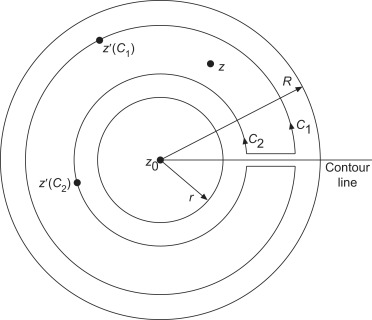
\includegraphics[width=0.7\textwidth]{LECTURE_10/laurent-series.jpg}
    \caption{Laurent Series}
    \label{fig:laurent_series}
\end{figure}

\begin{example}
    \begin{enumerate}
        \item $f(z) = \frac{H(z)}{(z - z_0)^m}$
        \item $f(z) = e^\frac{1}{z} = \sum_{n=0}^{\infty} \frac{z^{-n}}{n!}$
    \end{enumerate}
\end{example}

\chapter{Lecture 11: The Residue Theorem \& Applications} % Main chapter title

\begin{theorem}
    [Residue Theorem]
    Suppose $f$ is analytic on a simply connected domain $D$, except for a finite number of isolated singularities at $z_1, z_2, \cdots, z_n \in D$. Let $\gamma$ be a piecewise $C^1$, positively oriented, simple closed curve in $D$ which does not pass through any of the singularities. Then:
    \begin{equation}
        \boxed{\oint_{\gamma} f(z) dz = 2\pi i \sum_{z_k \text{ inside } \gamma} \text{Res}(f, z_k)}
    \end{equation}
\end{theorem}
\begin{figure}[H]
    \centering
    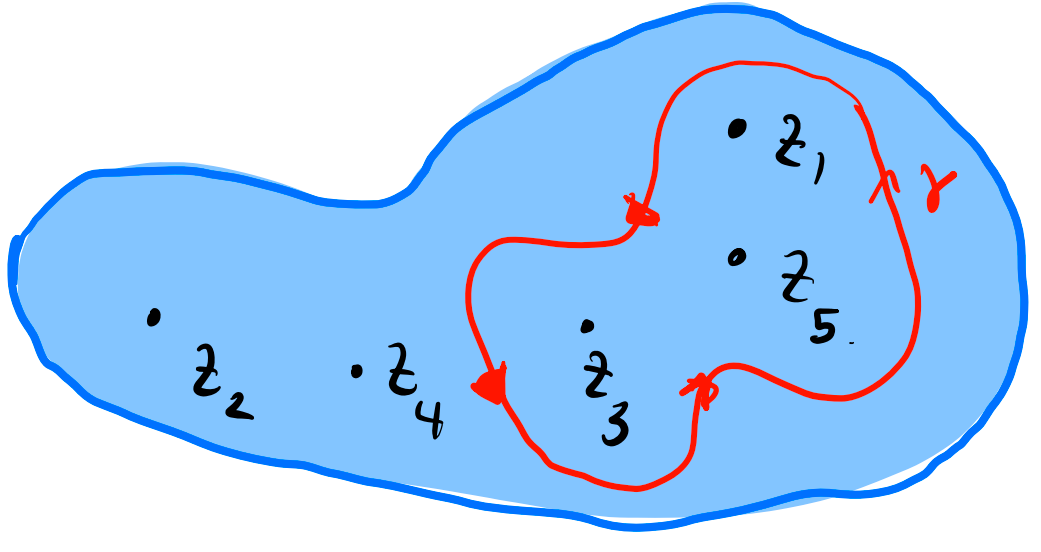
\includegraphics[width=0.4\textwidth]{LECTURE_11/residues.png}
    \caption{Residue Theorem}
    \label{fig:residue}
\end{figure}

\begin{proof}
    We'll use Green's Theorem with $\gamma = \partial \Omega$ where $\Omega$ is the region enclosed by $\gamma$.
    \begin{align*}
        \int_{\partial \Omega} f dz = i \int\int_{\Omega} \left( \frac{\partial f}{\partial x} - i\frac{\partial f}{\partial y} \right) dxdy
    \end{align*}
    We know that the integral of an analytic function over a closed curve is zero, so the only contributions to the integral are from the singularities inside $\Omega$. Let $\gamma_1, \gamma_2, \cdots, \gamma_n$ be disjoint, positively oriented, circles around singularities $z_1, z_2, \cdots, z_n$ respectively. We apply Green's theorem to get:
    \begin{equation*}
        \oint_{\gamma} f(z) dz = \sum_{k : z_k \text{ inside } \gamma} \oint_{\gamma_k} f(z) dz
    \end{equation*}
    \begin{figure}[H]
        \centering
        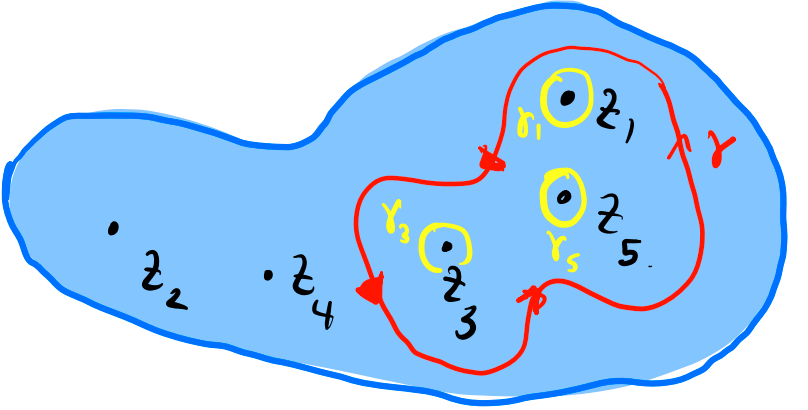
\includegraphics[width=0.4\textwidth]{LECTURE_11/residues-2.png}
        \caption{circles around $z_1, z_2, \cdots, z_n$}
        \label{fig:residue-2}
    \end{figure}

    To compute $\oint_{\gamma_k} f(z) dz$, we can write $f(z)$ as a Laurent series about $z_k$:
    \begin{equation}
        f(z) = \sum_{n = -\infty}^{\infty} a_n (z - z_k)^n = \frac{\text{Res}(f, z_k)}{z - z_k} + \text{regular terms}
    \end{equation}

    Now, we can compute the integral:
    \begin{align*}
        \oint_{\gamma_k} f(z) dz & = \oint_{\gamma_k} \frac{\text{Res}(f, z_k)}{z - z_k} dz + \oint_{\gamma_k} \text{regular terms } dz \\
    \end{align*}
    $\oint_{\gamma_k} \text{regular terms } dz$ is zero because when $n > -1$ the integrand is analytic and thus the integral of an analytic function over a closed curve is zero. When $n < -1$, the integrand is oscillatory and the integral is zero. So we are left with:
    \begin{align*}
        \oint_{\gamma_k} f(z) dz & = \oint_{\gamma_k} \frac{\text{Res}(f, z_k)}{z - z_k} dz \\
    \end{align*}
    Which resembles the Cauchy Integral Formula.
    \begin{align*}
        2\pi i f(z_0) & = \oint_{\gamma} \frac{f(z)}{z - z_0} dz
    \end{align*}
    So we can write:
    \begin{align*}
        \oint_{\gamma_k} f(z) dz & = \oint_{\gamma_k} \frac{\text{Res}(f, z_k)}{z - z_k} dz \\
                                 & = 2\pi i \text{Res}(f, z_k)
    \end{align*}
    Summing over all $z_k$ inside $\gamma$:
    \begin{align*}
        \oint_{\gamma} f(z) dz & = \sum_{k : z_k \text{ inside } \gamma} \oint_{\gamma_k} f(z) dz \\
                               & = 2\pi i \sum_{z_k \text{ inside } \gamma} \text{Res}(f, z_k)
    \end{align*}
\end{proof}

\begin{example}
    Compute:
    \begin{equation*}
        \int_{-\infty}^{\infty} \frac{x^2}{((1 + x^2)(4+ x^2))} dx
    \end{equation*}

    \textbf{Step 1:} Change to a complex integral:
    \begin{equation*}
        P(z) = z^2, \quad Q(z) = (1 + z^2)(4 + z^2)
    \end{equation*}

    \textbf{Step 2:} Choose a contour:
    \begin{figure}[H]
        \centering
        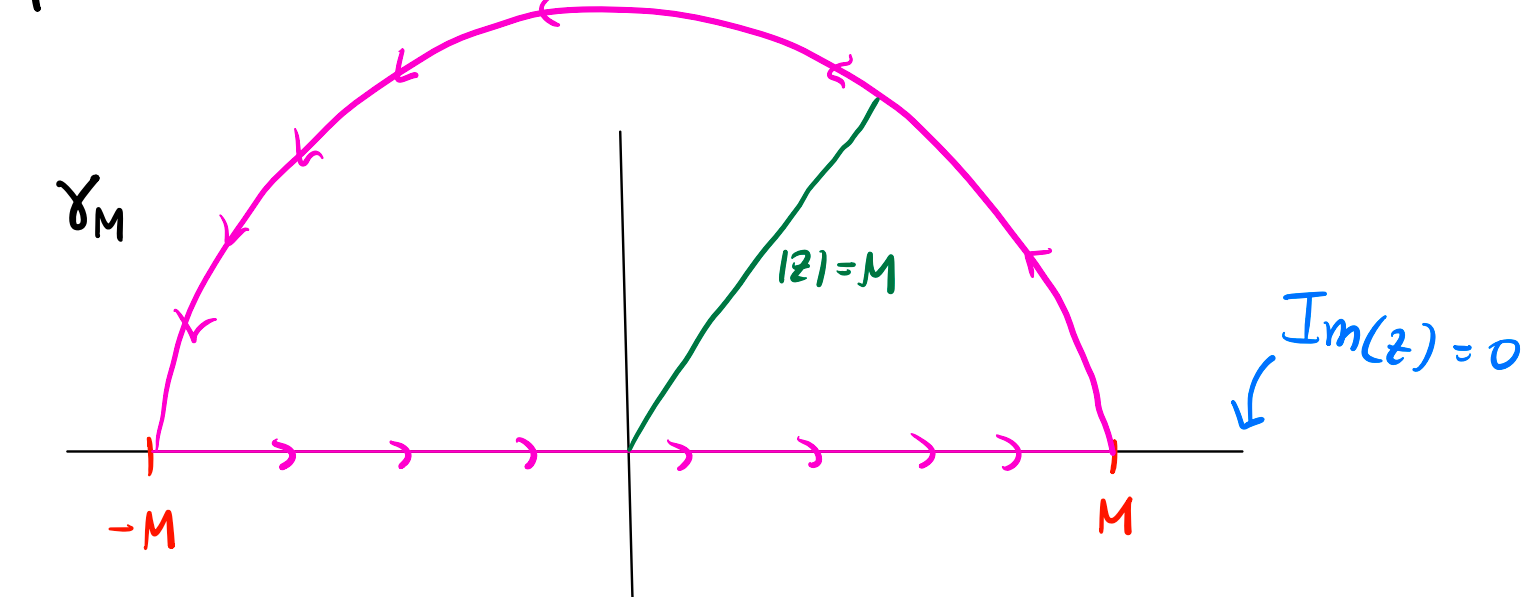
\includegraphics[width=0.4\textwidth]{LECTURE_11/contour.png}
        \caption{Contour}
        \label{fig:contour}
    \end{figure}
    Suppose $M$ is very large
    \begin{enumerate}
        \item $\int_{\gamma_M} \frac{P(z)}{Q(z)} dz$ can be computed by the residue formula.
        \item On the other hand:
              \begin{equation*}
                  \int_{\gamma_M} \frac{P(z)}{Q(z)} dz = \underbrace{\int_{-M}^{M}\frac{x^2}{(1 + x^2)(4 + x^2)} dx}_{\text{The integral we want}} + \int_{0}^{\pi} \frac{P(M e^{i\theta})}{Q(M e^{i\theta})} i M e^{i\theta} d\theta
              \end{equation*}
    \end{enumerate}
    \underline{Now}:
    \begin{align*}
        |P(Me^{i\theta})| & \leq M^2                                                \\
        |Q(Me^{i\theta})| & = |(Me^{i\theta})^2 + 1||(Me^{i\theta})^2 + 4|          \\
                          & \geq \frac{1}{10} M^4 \qquad \text{for a very large } M
    \end{align*}
    \underline{So}
    \begin{equation*}
        \left| \int_0^\pi \frac{P(Me^{i\theta})}{Q(Me^{i\theta})} i M e^{i\theta} d\theta \right| \leq 10 \pi \frac{M^3}{M^4} \to 0 \quad \text{as } M \to \infty
    \end{equation*}
    \textbf{\underline{Thus}}
    \begin{equation*}
        \int_{-\infty}^{\infty} \frac{x^2}{(1 + x^2)(4 + x^2)} dx = \lim_{M \to \infty} \int_{\gamma_M} \frac{P(z)}{Q(z)} dz
    \end{equation*}
    Which can be computed using the residue formula. \\
    $Q(z)$ has zeroes at $z = \pm i, \pm 2i$. only $+i, +2i$ are inside $\gamma_M$ for large $M$. So:
    \begin{align*}
        \boxed{z = i} \quad \rightarrow\quad \frac{z^2}{(z + i)(z-i)(z^2 + 4)}  & = \frac{1}{z - i}\left[\frac{z^2}{(z + i)(z^2 + 4)}\right]   \\
        \text{So Res}(f, i)                                                     & = \frac{i^2}{(i + i)(i^2 + 4)} = \frac{-1}{6i}               \\
        \boxed{z = 2i}\quad \rightarrow \quad \frac{z^2}{(z + i)(z-i)(z^2 + 4)} & = \frac{1}{z - 2i}\left[\frac{z^2}{(z + 2i)(z^2 + 1)}\right] \\
        \text{So Res}(f, 2i)                                                    & = \frac{-4}{4i(-4 + 1)} = \frac{1}{3i}
    \end{align*}
    \underline{Thus, } for a large $M$:
    \begin{align*}
        \int_{\gamma_M} \frac{P(z)}{Q(z)} dz & = 2\pi \left(\frac{-1}{6i} + \frac{1}{3i}\right) \\
                                             & = \frac{\pi}{3}
    \end{align*}
\end{example}

\begin{theorem}
    [Solving Residue Problems]
    \underline{What do we need?} \\
    Polynomials $P(z), Q(z)$ such that:
    \begin{enumerate}
        \item $Q(z)$ has no zeroes on the line $\Re(z) = 0$.
        \item[] Why?
              \begin{itemize}
                  \item To apply the Residue Theorem to the contour shown in figure \ref{fig:contour}.
              \end{itemize}
        \item $\deg(Q) \geq \deg(P) + 2$.
        \item[] Why?
              \begin{itemize}
                  \item To ensure that the integral over the arc goes to zero.
                  \item $\int_0^\pi \frac{P(Me^{i\theta})}{Q(Me^{i\theta})} i M e^{i\theta} d\theta \to 0$ as $M \to \infty$.
              \end{itemize}
    \end{enumerate}

\end{theorem}

\begin{proposition}
    $P, Q$ polynomials that are real-valued on $\Im(z) = 0$ and $\deg(Q) \geq \deg(P) + 2$, then if $Q(x) \neq 0$ for all $x \in \mathbb{R}$, then:
    \begin{equation}
        \int_{-\infty}^{\infty} \frac{P(x)}{Q(x)} dx = 2\pi i \sum_{z_j \in U} \text{Res}\left(\frac{P(z)}{Q(z)}, z_j\right)
    \end{equation}
    Where $ U = \{z_j : \Im(z_j) > 0\}$.
    \label{prop:residue}
\end{proposition}

\begin{proof}
    Take the contour $\gamma_M$ as shown in figure \ref{fig:contour}, for a large $M$, the residue theorem applies and all zeroes of $Q \in \{z : \Im(z) > 0\}$ are inside $\gamma_M$. \\
    \underline{\textbf{Claim:}} for $M$ large:
    \begin{itemize}
        \item $|Q(Me^{i\theta})| \geq c_1M^{\deg(Q)}$ for some $c_1 > 0$.
        \item $|P(Me^{i\theta})| \leq c_2M^{\deg(P)}$ for some $c_2 > 0$.
    \end{itemize}
    This can be proved using the triangle inequality:
    \begin{align*}
        PERFORM THE INEQUALITY
    \end{align*}
    Since $\deg(P) + 1 - \deg(Q) \leq -1$ by assumption. \\
    Now apply the residue theorem to $\gamma_M$:
    \begin{align*}
        \int_{\gamma_M} \frac{P(z)}{Q(z)} dz         & = 2\pi i \sum_{z_j \in U} \text{Res}\left(\frac{P(z)}{Q(z)}, z_j\right) \\
        \int_{-\infty}^{\infty} \frac{P(x)}{Q(x)} dx & = 2\pi i \sum_{z_j \in U} \text{Res}\left(\frac{P(z)}{Q(z)}, z_j\right)
    \end{align*}
\end{proof}

\section{Integrals Involving Trigonometric Functions}

\begin{proposition}
    Suppose $R$ is a rational function (ratio of two polynomials) that is real on $\Im(z) = 0$. We can integrate $(x)\sin(x)$ or $R(x)\cos(x)$ over $(-\infty, \infty)$ by integrating
    $$\Re{R(z)e^{iz}}, \quad \Im{R(z)e^{iz}}$$
    Respectively over the contour shown in figure \ref{fig:contour}.
\end{proposition}

\begin{example}
    Compute:
    $$\int_{-\infty}^{\infty} \frac{\cos(x)}{x^2 + \alpha^2} dx \quad \text{for } \alpha > 0$$

    \textbf{Step 1:} Change to a complex integral and replace $\cos(x)$ with $\Re{e^{iz}}$

    \begin{align*}
        P(z) & = e^{iz}         \\
        Q(z) & = z^2 + \alpha^2
    \end{align*}

    \textbf{Step 2:} $\deg(Q) \geq \deg(P) + 2$.
    \begin{align}
        \lim_{z \to \infty} P(z) & = \lim_{z \to \infty} e^{iz} = 1              \\
        \lim_{z \to \infty} Q(z) & = \lim_{z \to \infty} z^2 + \alpha^2 = \infty
        \therefore \deg(Q)       & \geq \deg(P) + 2
    \end{align}

    \textbf{Step 3:} Choose a contour as shown in figure \ref{fig:contour}. Because we satisfy the conditions of proposition \ref{prop:residue}, we can apply it to compute the integral.

    \begin{align}
        \therefore \int_{-\infty}^{\infty} \frac{\cos(x)}{x^2 + \alpha^2} dx & = \Re{\left(\lim_{M\to \infty}\oint_{\gamma_M} \frac{e^{iz}}{z^2 + \alpha^2} dz\right)}               \\
                                                                             & = \Re{\left(2\pi i \sum_{z_j \in U} \text{Res}\left(\frac{e^{iz}}{z^2 + \alpha^2}, z_j\right)\right)}
    \end{align}

    \textbf{Step 4:} Compute the residues:
    $z^2 + \alpha^2 = 0 \implies z = \pm i\alpha$ and only $i\alpha$ is in $\gamma_M$ for large $M$.
    \begin{align}
        \text{Res}\left(\frac{e^{iz}}{z^2 + \alpha^2}, i\alpha\right) & = \lim_{z \to i\alpha} (z - i\alpha)\frac{e^{iz}}{z^2 + \alpha^2} \\
                                                                      & = \frac{e^{i(i\alpha)}}{2i\alpha} = \frac{e^{-\alpha}}{2i\alpha}
    \end{align}

    \textbf{Step 5:} Compute the integral:

    \begin{align}
        \int_{-\infty}^{\infty} \frac{\cos(x)}{x^2 + \alpha^2} dx & = \Re{\left(2\pi i \sum_{z_j \in U} \text{Res}\left(\frac{e^{iz}}{z^2 + \alpha^2}, z_j\right)\right)} \\
                                                                  & = \Re{\left(2\pi i \frac{e^{-\alpha}}{2i\alpha}\right)}                                               \\
                                                                  & = \frac{\pi e^{-\alpha}}{\alpha}
    \end{align}
\end{example}

\subsection{There is another example in the notes... But I'm tired....}

\chapter{Homework 5} % Main chapter title


\begin{example}
    Solve the integral:
    $$f(z) = \frac{z^2}{1 - z^2}, \quad z_0 = 1$$

    \textbf{Solution:}
    \begin{align*}
        2\pi i \text{Res}(f, z_0) & = \int_{\gamma} f(z) dz                             \\
                                  & = \int_{\gamma} \frac{z^2}{(z - 1)(z + 1)} dz       \\
                                  & = \int_{\gamma} \frac{-\frac{z^2}{z + 1}}{z - 1} dz
    \end{align*}
    Say, $g(z) = -\frac{z^2}{z + 1}$, then using Cauchy's Integral Formula:
    \begin{align*}
        2\pi i \text{Res}(f, z_0) & = \int_{\gamma} \frac{-\frac{z^2}{z + 1}}{z - 1} dz \\
                                  & = -2\pi i g(1) = -\pi i                             \\
                                  & = 2\pi i \left( -\frac{1}{2} \right) = -\pi i       \\
                                  & \therefore \text{Res}(f, z_0) = -\frac{\pi i}{2}
    \end{align*}
\end{example}

\begin{example}
    Solve the integral:
    $$\int_{-\infty}{\infty} \frac{x^2}{x^4 + 5x^2 + 4} dx$$

    \textbf{Solution:}

    First, we factor the denominator:
    \begin{align*}
        x^4 + 5x^2 + 4 & = (x^2 + 4)(x^2 + 1)             \\
                       & = (x + 2i)(x - 2i)(x + i)(x - i)
    \end{align*}
    We only care about two residues here, because the other two are not in the upper half plane. So we have:
    \begin{align*}
        \int_{\gamma_R}\frac{z^2}{z^4 + 5z^2 + 4} dz & = \frac{1}{2\pi i}(\text{Res}(f, i) + \text{Res}(f, 2i))                              \\
                                                     & = 2\pi (\frac{1}{6} - \frac{2i}{6}) = \frac{-\pi}{3} + \frac{2\pi}{3} = \frac{\pi}{3}
    \end{align*}
    Next, let's find the residues at $i$ and $2i$:
    \begin{align*}
        \text{Res}(f, i) & = \frac{1}{2\pi i}\int_{\gamma} f(z) dz = \frac{1}{2\pi i}\int_{\gamma} \frac{z^2}{(z + 2i)(z - 2i)(z + i)(z - i)} dz \\
                         & = \frac{1}{2\pi i}\int_{\gamma} \frac{\frac{z^2}{(z + 2i)(z - 2i)(z+2i)}}{z-i}dz                                      \\
                         & = \frac{1}{2\pi i}2\pi g(i) = \frac{i^2}{(i + 2i)(i - 2i)(i + 2i)} = -\frac{1}{6}
    \end{align*}
    \begin{align*}
        \text{Res}(f, 2i) & = \frac{1}{2\pi i}\int_{\gamma} f(z) dz = \frac{1}{2\pi i}\int_{\gamma} \frac{z^2}{(z + 2i)(z - 2i)(z + i)(z - i)} dz \\
                          & = \frac{1}{2\pi i}\int_{\gamma} \frac{\frac{z^2}{(z + 2i)(z - i)(z+2i)}}{z-2i}dz                                      \\
                          & = g(2 i)  = \frac{(2 - i)^2}{(2i + 2i)(2i - i)(2i + i)} = \frac{4}{12i}
    \end{align*}
    \begin{align*}
        P(z) & = a_nz^n + a_{n-1}z^{n-1} + \cdots + a_0                      \\
             & \lim_{|z| \to \infty} \left| \frac{P(z)}{z^n} \right| = |a_n| \\
    \end{align*}
    $R$ is large enough so that $|f(z)| < \epsilon$ for $|z| > R$, so we have:
    \begin{align*}
        \frac{1}{2} |a_n| \leq \left|\frac{P(z)}{z^n}\right| \leq 2|a_n| \\ \quad \text{for} \quad z = \alpha_R (z), \quad |z^n| = R^n \\
    \end{align*}

    \begin{align*}
        P(z) & = z^2                                                            \\
        Q(z) & = z^4 + 5z^2 + 4                                                 \\
        \left|\frac{P(z)}{Q(z)}\right| \leq \frac{2 |1| R^2}{\frac{1}{2}|1|R^4} \\
             & = 4R^{-2}
    \end{align*}

    \begin{align*}
        \left|\int_{\alpha_R} f(z)dz\right| & \leq \int_{\alpha_R} \left|\frac{P(z)}{Q(z)}\right| dz    \\
                                            & \leq \int_{\alpha_R} 4R^{-2} dz                           \\
                                            & = 4R^{-2} \int_{\alpha_R} dz                              \\
                                            & = 4R^{-2} \pi R                                           \\
                                            & = \frac{4\pi}{R} \to 0 \quad \text{as} \quad R \to \infty
    \end{align*}
\end{example}

\begin{proposition}
    In general if $f = \frac{P(z)}{Q(z)}$ where $P(z)$ and $Q(z)$ are polynomials and $\deg Q \geq \deg P + 2$, then:
    \begin{align*}
        I & = \int_{-\infty}^{\infty} \frac{P(x)}{Q(x)} dx   \\
        I & = 2\pi i \sum_{\text{Im} z > 0} \text{Res}(f, z)
    \end{align*}
    ensure that $Q \neq 0$
\end{proposition}

\chapter{Midterm Review}

\chapter{Lecture 12: Contour Integrals}

\begin{example}
    Compute:
    $$\int_{0}^{\infty} \frac{\sin^2 x}{x^2} dx$$

    \textbf{step 1:} Replace with a complex function:
    \begin{align*}
        2\sin^2 x                                 & = 1 - \cos 2x                                                                       \\
        \int_{0}^{\infty} \frac{\sin^2 x}{x^2} dx & = \frac{1}{2} \int_{-\infty}^{\infty} \frac{\sin^2 x}{x^2} dx                       \\
                                                  & = \frac{1}{4} \int_{-\infty}^{\infty} \frac{1 - \cos 2x}{x^2} dx                    \\
                                                  & = \frac{1}{4} \int_{-\infty}^{\infty} \frac{1 - \cos 2z}{z^2} dz                    \\
                                                  & = \Re \left( \frac{1}{4} \int_{-\infty}^{\infty} \frac{1 - e^{2iz}}{z^2} dz \right)
    \end{align*}

    \textbf{step 2:} Choose the right contour:
    Previously, we used a semi-circle in the upper half plane with the condition that there are no zeroes on the line $Im(z) = 0$. This time, there is a zero at $z = 0$. So, we need to use a contour that excludes this zero. We can use a semi-circle in the upper half plane with a small semi-circle around the origin removed (half-keyhole contour) as seen in the figure below.
    \begin{figure}[H]
        \centering
        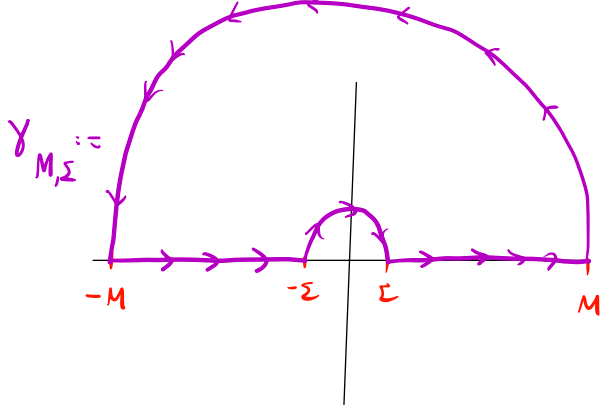
\includegraphics[width=0.5\textwidth]{LECTURE_12/half-keyhole.png}
        \caption{Half-keyhole contour}
        \label{fig:half-keyhole}
    \end{figure}

    \textbf{step 3:} If there are singularities in the contour, find their residues:
    There are no singularities in the contour, so:
    \begin{align}
        \int_{\gamma_{M,\epsilon}} f(z)dz = 0
    \end{align}

    \textbf{step 4:} Evaluate the consequences of the contour:
    By Cauchy's Integral Formula, we know that the integral around a closed loop is zero for a function that is analytic in the region enclosed by the loop.
    Say $f(z) = \frac{1 - e^{2iz}}{z^2}$, then we can write:
    \begin{align*}
        0 = \int_{\gamma_{M,\epsilon}} f(z)dz & = \int_{\{z=Me^{i\theta}, \theta \in [0, \pi]\}} f(z)dz       & (I)   \\
                                              & + \int_{z = \epsilon e^{i\theta}, \theta \in [0, \pi]} f(z)dz & (II)  \\
                                              & + \int_{-M}^{-\epsilon} f(z)dz + \int_{\epsilon}^{M} f(z)dz   & (III) \\
    \end{align*}
    We know from last lecture that $(I) = 0$ as $M \to \infty$ and as $M \to \infty, \epsilon \to 0$, $(III) \to \int_{-\infty}^{\infty} f(z)dz$ (the integral we want to compute). So, we can write:
    \begin{align*}
        \int_{-M}^{-\epsilon} f(z)dz + \int_{\epsilon}^{M} f(z)dz & = -\int_{z = \epsilon e^{i\theta}, \theta \in [0, \pi]} f(z)dz \\
        (III)                                                     & = -(II)
    \end{align*}
    We compute $(II)$ explicitly, let $z = \epsilon e^{i\theta}$:
    \begin{align*}
        (II) & = \int_{z = \epsilon e^{i\theta}, \theta \in [0, \pi]} f(z)dz                                                \\
             & = \int_{\pi}^{0} f(\epsilon e^{i\theta})d(\epsilon e^{i\theta})                                              \\
             & = \int_{\pi}^{0} f(\epsilon e^{i\theta})i\epsilon e^{i\theta}d\theta                                         \\
             & = \int_{\pi}^{0} \frac{1 - e^{2i\epsilon e^{i\theta}}}{(\epsilon e^{i\theta})^2}i\epsilon e^{i\theta}d\theta \\
             & = \int_{\pi}^{0} \frac{1 - e^{2i\epsilon e^{i\theta}}}{\epsilon e^{i\theta}}id\theta                         \\
    \end{align*}
    Now let's use the Taylor expansion of $e^{2i\epsilon e^{i\theta}}$:
    \begin{align*}
        \rightarrow e^{2i\epsilon e^{i\theta}}                                            & = 1 + 2i\epsilon e^{i\theta} - \frac{4(\epsilon e^{i\theta})^2}{2} + \frac{8i(\epsilon e^{i\theta})^3}{6} \ldots \\
        \rightarrow 1 - e^{2i\epsilon e^{i\theta}}                                        & = -2i\epsilon e^{i\theta} + \frac{4(\epsilon e^{i\theta})^2}{2} - \frac{8i(\epsilon e^{i\theta})^3}{6} \ldots    \\
        \rightarrow \frac{1 - e^{2i\epsilon e^{i\theta}}}{\epsilon e^{i\theta}}           & = -2i + 2\epsilon e^{i\theta} - \frac{4\epsilon e^{i\theta}}{2} + \frac{8i(\epsilon e^{i\theta})^2}{6} \ldots    \\
        \lim_{\epsilon \to 0} \frac{1 - e^{2i\epsilon e^{i\theta}}}{\epsilon e^{i\theta}} & = -2i                                                                                                            \\
        \therefore (II)                                                                   & = \int_{\pi}^{0} -2i^2 d\theta = 2\pi
    \end{align*}
    So, we have:
    \begin{align}
        \int_{-\infty}^{\infty} \frac{1 - e^{2iz}}{z^2} dz & = \Re \left( \frac{1}{4} \int_{-\infty}^{\infty} \frac{1 - e^{2iz}}{z^2} dz \right) \\
                                                           & = \Re \left( \frac{1}{4} \cdot 2\pi \right) = \frac{\pi}{2}
    \end{align}
\end{example}

\section{Integrals Involving the Log or Fractional Powers}
\begin{example}
    Compute:
    $$\int_{0}^{\infty} \frac{\log x}{(1 + x^2)^2} dx$$

    \textbf{step 1:} Replace with a complex function:
    \begin{align*}
        \int_{0}^{\infty} \frac{\log x}{(1 + x^2)^2} dx & = \int_{0}^{\infty} \frac{\log z}{(1 + z^2)^2} dz
    \end{align*}
    Because we're in the complex plane now, we must define a branch cut for the logarithm. We can choose the negative real axis as the branch cut, so $\Im{\log z} \in (-\frac{\pi}{2}, \frac{3\pi}{2})$.

    \textbf{step 2:} Choose the right contour:
    We want to use a contour that excludes the branch cut and the part of the real axis where the integrand is not defined ($z = 0$). We can use a semi-circle in the upper half plane with a small semi-circle around the origin removed (half-keyhole contour) as seen in figure \ref{fig:half-keyhole}.

    \textbf{step 3:} If there are singularities in the contour, find their residues:
    There are singularities where $1 + z^2 = 0 \rightarrow z = \pm i$. We can see that the singularity at $z = i$ is enclosed by the contour, so we need to find the residue at $z = i$, which is a pole of order 2. We can write:

    \begin{align}
        \text{Res}(f,z_k) & = \frac{1}{(m - 1)!}\lim_{z \to z_k} \frac{d^{m-1}}{dz^{m-1}} \left( (z - z_k)^m f(z) \right)        \\
        \text{Res}(f,i)   & = \frac{1}{1!}\lim_{z \to i} \frac{d}{dz} \left( (z - i)^2 \frac{\log z}{(z + i)^2(z - i)^2} \right) \\
                          & = \lim_{z \to i} \frac{d}{dz} \left( \frac{\log z}{(z + i)^2} \right)                                \\
                          & = \lim_{z \to i} \frac{1}{z} \cdot \frac{1}{(z + i)^2} - \frac{2\log z}{(z + i)^3}                   \\
                          & = \frac{1}{i} \cdot \frac{1}{(2i)^2} - \frac{2\log i}{(2i)^3}                                        \\
                          & = \frac{1}{-4i} + \frac{\log i}{4i}                                                                  \\
                          & = \frac{1}{-4i} + \frac{(\log 1 + i\pi/2)}{4i}                                                       \\
                          & = \frac{1}{-4i} + \frac{i\pi/2}{4i}                                                                  \\
                          & = \frac{\pi/2 + i}{4}
    \end{align}

    Therefore we can state:
    \begin{align}
        \int_{\gamma_{M,\epsilon}} f(z)dz & = 2\pi i \cdot \frac{\pi/2 + i}{4} \\
                                          & = \frac{\pi^2}{4}i - \frac{\pi}{2}
    \end{align}

    \textbf{step 4:} Find the consequences of the contour:

    We can write:
    \begin{align*}
        0 = \int_{\gamma_{M,\epsilon}} f(z)dz & = \int_{\{z=Me^{i\theta}, \theta \in [0, \pi]\}} f(z)dz       & (I)   \\
                                              & + \int_{z = \epsilon e^{i\theta}, \theta \in [0, \pi]} f(z)dz & (II)  \\
                                              & + \int_{-M}^{-\epsilon} f(z)dz + \int_{\epsilon}^{M} f(z)dz   & (III) \\
    \end{align*}
    We can see that:
    \begin{align}
        (I)                                             & = 0 \text{ as } M \to \infty                                                                                                                     \\
        (II)                                            & = \lim_{\epsilon \to 0}\int_{0}^{\infty} f(\epsilon e^{i \theta})\epsilon i e^{i \theta} d\theta                                                 \\
                                                        & = \lim_{\epsilon \to 0} \int_{0}^{\infty} \frac{\log \epsilon + i\theta}{(1 + \epsilon^2 e^{2i\theta})^2} \epsilon i e^{i \theta} d\theta = 0    \\
        (III)                                           & = \int_{-M}^{-\epsilon} f(z)dz + \int_{\epsilon}^{M} f(z)dz                                                                                      \\
        \frac{\pi^2}{4}i - \frac{\pi}{2}                & =\int_{-M}^{-\epsilon} \frac{\log |z| + i\pi}{(1 + z^2)^2}dz + \int_{\epsilon}^{M} \frac{\log |z|}{(1 + z^2)^2}dz                                \\
        \frac{\pi^2}{4}i - \frac{\pi}{2}                & =i\pi \int_{-M}^{-\epsilon} \frac{1}{(1 + z^2)^2}dz + 2\underbrace{\int_{\epsilon}^{M} \frac{\log |z|}{(1 + z^2)^2}dz}_{\text{Integral we want}} \\
        \int_{0}^{\infty} \frac{\log x}{(1 + x^2)^2} dx & = -\frac{\pi}{4}
    \end{align}
\end{example}

\chapter{Lecture 13: More Contour Integration}

\begin{example}
    Find the value of:
    $$\int_{0}^{\infty} \frac{x^{1/3}}{x^2 + 4x + 8} dx$$

    \textbf{step 1:} Replace with a complex function:
    Let $f(z) = \frac{z^{1/3}}{z^2 + 4z + 8}$, then:
    \begin{align*}
        \int_{0}^{\infty} \frac{x^{1/3}}{x^2 + 4x + 8} dx & = \int_{-\infty}^{\infty} \frac{z^{1/3}}{z^2 + 4z + 8} dz             \\
                                                          & = \int_{-\infty}^{\infty} \frac{e^{\frac{1}3\log z}}{z^2 + 4z + 8} dz
    \end{align*}

    \textbf{step 2:} Choose the right contour:
    \textbf{NOTE: } $\int_{-\infty}^{0} \frac{|z|^{1/3}}{z^2 + 4z + 8} dz \neq \int_{0}^{\infty} \frac{z^{1/3}}{z^2 + 4z + 8} dz$ so, $\int_{-\infty}^{\infty} \frac{z^{1/3}}{z^2 + 4z + 8} \neq 2\int_{0}^{\infty} \frac{x^{1/3}}{x^2 + 4x + 8} dx$ because $z^2 + 4x + 8$ is not even.
    (There's an absolute value in the numerator because we'd be able to evaluate the imaginary part of the logarithm explicitly)
    Therefore a half-keyhole contour is not appropriate. We can use a full keyhole contour as seen in the figure below.

    \begin{figure}[H]
        \centering
        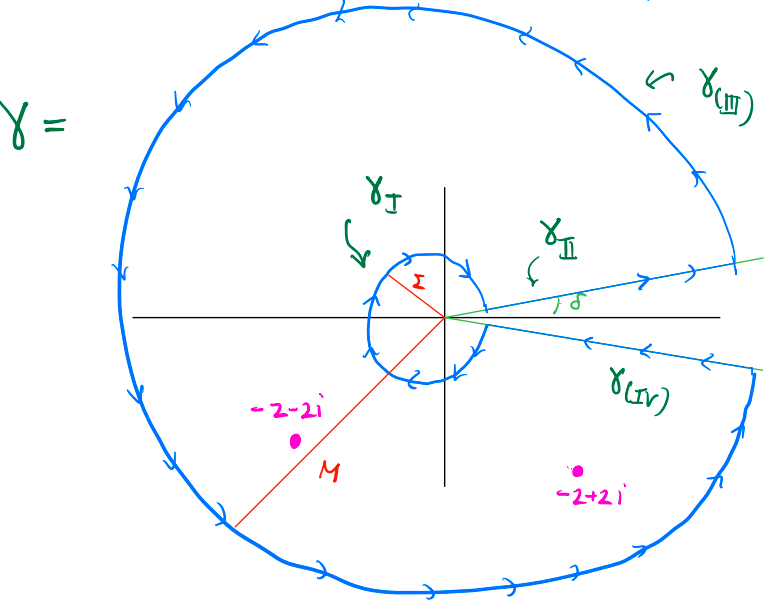
\includegraphics[width=0.75\textwidth]{LECTURE_13/keyhole-contour.png}
    \end{figure}

    \textbf{Step 2.5:} Choose the branch cut:
    We need to choose a branch cut over which $z^{1/3}$ is analytic. We can choose the positive real axis so that $\arg(z) \in [0, 2\pi)$.

    \textbf{step 3:} If there are singularities in the contour, find their residues:
    There are singularities at $z = -2 \pm 2i$. They are both enclosed by the contour, so we need to find the residues at both points. We can write:
    \begin{align*}
        \rightarrow f(z)                   & = \frac{z^{1/3}}{(z + 2 - 2i)(z + 2 + 2i)}                                      \\
        \text{Res}(f,z_k)                  & = \lim_{z \to z_k} (z - z_k) f(z)                                               \\
        \text{Res}(f,-2 + 2i)              & = \lim_{z \to -2 + 2i} (z - (-2 + 2i)) \frac{z^{1/3}}{(z + 2 - 2i)(z + 2 + 2i)} \\
                                           & = \lim_{z \to -2 + 2i} \frac{z^{1/3}}{(z + 2 - 2i)}                             \\
                                           & = \frac{(-2 + 2i)^{1/3}}{(-2 + 2i + 2 - 2i)}                                    \\
                                           & = \frac{2^{1/3}e^{i\pi/4}}{4} = \frac{e^{i\pi/4}}{2^{2/3}}                      \\
        \text{Res}(f,-2 - 2i)              & = \lim_{z \to -2 - 2i} (z - (-2 - 2i)) \frac{z^{1/3}}{(z + 2 - 2i)(z + 2 + 2i)} \\
                                           & = \lim_{z \to -2 - 2i} \frac{z^{1/3}}{(z + 2 + 2i)}                             \\
                                           & = \frac{(-2 - 2i)^{1/3}}{(-2 - 2i + 2 + 2i)}                                    \\
                                           & = \frac{2^{1/3}e^{-i\pi/4}}{4} = \frac{e^{-i\pi/4}}{2^{2/3}}                    \\
        \therefore \text{Res}(f,-2 \pm 2i) & = \frac{e^{\pm i\pi/4}}{2^{2/3}}
    \end{align*}
    We can compute the integral:
    \begin{align*}
        i\pi/4\int_{\gamma_{M,\epsilon,\delta}} f(z)dz & = 2\pi i \left( \frac{e^{i\pi/4}}{2^{2/3}} + \frac{e^{-i\pi/4}}{2^{2/3}} \right) \\
    \end{align*}
    \textbf{step 4:} Find the consequences of the contour:
    Recall Example \ref{ex:keyhole} From chapter 5, lecture 4 for the parametrization of the keyhole contour:
    \begin{align*}
        \gamma (t) = \begin{cases}
                         Me^{i\theta}          & \delta \leq \theta \leq 2\pi - \delta \\
                         te^{i(2\pi - \delta)} & M \leq t \leq \epsilon                \\
                         \epsilon e^{i\theta}  & 2\pi - \delta \leq \theta \leq \delta \\
                         te^{i\delta}          & \epsilon \leq t \leq M
                     \end{cases}
    \end{align*}
    From the residue theorem and the contour in the figure above, we can write:
    \begin{align*}
        i\pi/4\int_{\gamma_{M,\epsilon,\delta}} f(z)dz & = \int_{\gamma_I} f(z)dz + \int_{\gamma_{II}} f(z)dz + \int_{\gamma_{III}} f(z)dz + \int_{\gamma_{IV}} f(z)dz
    \end{align*}
    By previous arguments, as $M \to \infty$ and $\epsilon \to 0$, we can write:
    \begin{align*}
        \int_{\gamma_{I}} f(z)dz   & = 0 \\
        \int_{\gamma_{III}} f(z)dz & = 0 \\
    \end{align*}
    The other two integrals can be computed as:
    \begin{align*}
        \int_{\gamma_{II}} f(z)dz & = \int_{\epsilon}^{M} f(r e^{i\delta})r i e^{i\delta} dr                                                              \\
                                  & = \int_{\epsilon}^{M} \frac{r^{1/3}e^{i\delta/3}}{(r e^{i\delta} + 2 - 2i)(r e^{i\delta} + 2 + 2i)}r i e^{i\delta} dr \\
                                  & \text{As } M \to \infty, \epsilon \to 0, \delta \to 0                                                                 \\
                                  & = \int_{0}^{\infty} \frac{r^{1/3}}{(r + 2 - 2i)(r + 2 + 2i)}r i dr                                                    \\
    \end{align*}
    On the other hand:
    \begin{align*}
        \int_{\gamma_{IV}} f(z)dz & = \int_{M}^{\epsilon} f(r e^{i\delta})r i e^{i\delta} dr                                                                                              \\
                                  & = \int_{M}^{\epsilon} \frac{r^{1/3}e^{i(2\pi -\delta)/3}}{(r e^{i(2\pi -\delta)} + 2 - 2i)(r e^{i(2\pi -\delta)} + 2 + 2i)}r i e^{i(2\pi -\delta)} dr \\
                                  & \text{As } M \to \infty, \epsilon \to 0, \delta \to 0                                                                                                 \\
                                  & = \int_{\infty}^{0} \frac{r^{1/3}e^{i2\pi/3}}{(r + 2 + 2i)(r + 2 - 2i)}r i dr                                                                         \\
                                  & = e^{i2\pi/3}\int_{0}^{\infty} \frac{r^{1/3}}{(r + 2 - 2i)(r + 2 + 2i)}r i dr                                                                         \\
    \end{align*}
    Therefore:
    \begin{align*}
        \left[\int_{0}^{\infty} \frac{r^{1/3}}{(r + 2 - 2i)(r + 2 + 2i)}r i dr\right]\left[1 - e^{i2\pi/3}\right] & = i\pi/4\int_{\gamma_{M,\epsilon,\delta}} f(z)dz                                                         \\
        \int_{0}^{\infty} \frac{r^{1/3}}{(r + 2 - 2i)(r + 2 + 2i)}r i dr                                          & = \frac{2\pi i}{1 - e^{i2\pi/3}} \left( \frac{e^{i\pi/4}}{2^{2/3}} + \frac{e^{-i\pi/4}}{2^{2/3}} \right) \\
    \end{align*}
\end{example}

\begin{proposition}
    [Keyhole Contour Integral]
    Use a keyhole contour to evaluate real integrals with logarithms or fractional powers where the integrand is not even.
    $$\left[\int_{0}^{\infty} f(x)dx\right](1 - e^{i\theta}) = \int_{\gamma_{M,\epsilon,\delta}} f(z)dz = 2\pi i \sum \text{Res}(f,z_k)$$
    Where $\gamma_{M,\epsilon,\delta}$ is the sum of the residues of the singularities enclosed by the contour. $\theta = i\arg z \times \text{fractional power of z}$ for a fractional power of $z$.
\end{proposition}

\section{Analytic Functions as Mappings (Chap. 3)}

\subsection{3.1 - The Zeroes of an Analytic Function}

\begin{lemma}
    Recall that if $f(z)$ is not identically $0$ on a domain $D$ and $f(z_0) = 0$ for some $z_0 \in D$, then $f(z)$ has a pole at $z_0$ of order $m$ if $f(z) = (z - z_0)^m g(z)$ where $g(z)$ is analytic and $g(z_0) \neq 0$.
\end{lemma}

\begin{proposition}
    [The Identity Theorem]
    If $f(z)$ is analytic on a domain $D$ and there exists a sequence of points $\{z_n\}$ in $D$ such that $f(z_n) = 0$ and $z_n \to z_0 \in D$, then $f(z) = 0$ for all $z \in D$.
    \textbf{Alternatively:}
    If $f$ is analytic on $D$, not identically zero, and $f(z_0) = 0$ for some $z_0 \in D$, then $\exists \delta > 0 | z_0$ is the only zero of $f \in \{z \in D | |z - z_0| < \delta\}$.
\end{proposition}

\begin{proof}
    Suppose $f$ is analytic, $f(z_0) = $ and $\exists z_n \in \{|z_0 - z| < \frac{1}n\}$ such that $f(z_n) = 0$ this would mean:
    \begin{align*}
        f(z)   & = \sum_{n=0}^{\infty} a_n(z - z_0)^n               \\
        f(z_0) & = a_0(z_0 - z_0)^0 + a_1(z_0 - z_0)^1 + \ldots = 0
               & = a_0\times 0^0                                    \\
        0 = a_0 \times 1
    \end{align*}
    If $a_0, a_1, \ldots a_{n-1}$ are all $0$ then:
    \begin{align*}
        g(z)   & = \frac{f(z)}{(z - z_0)^n} = a_n + a_{n+1}(z - z_0) + \ldots = 0 \\
        g(z_n) & = \frac{f(z_n)}{(z_n - z_0)^n} = \frac{0}{(z_n - z_0)^n} = 0     \\
        a_n = 0
    \end{align*}
\end{proof}
\begin{figure}[H]
    \centering
    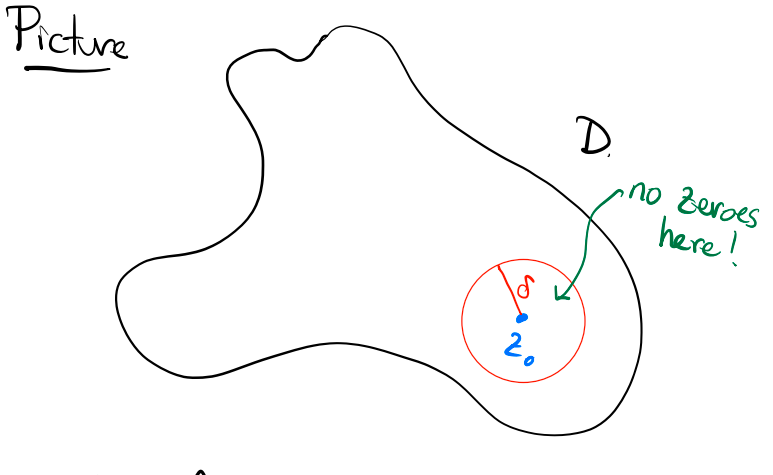
\includegraphics[width=0.75\textwidth]{LECTURE_13/pic.png}
    \caption{$\delta$ where no other zeroes exist}
\end{figure}

\begin{proposition}
    If $D$ is a bounded domain (i.e. $D \subset \{|z| < M\}$ for some $M$) then $f$ has only finitely many zeroes. Thus, we can count them. This can be done using the residue theorem.
\end{proposition}

\begin{proof}
    Zeroes are isolated in $D$ so they must be at least some $\delta$ apart. If $D$ then there is only finite space for zeroes and thus, there are only finitely many zeroes.
\end{proof}

\begin{theorem}
    [Argument Principle]
    Suppose $h$ is analytic in a domain $D$ except for a finite number of isolated poles. Let $\gamma$ be a piecewise $C^{1}$, positively oriented, simple closed curve in $D$, which does not pass through any pole or zero of $h$, and such that inside$(\gamma) \subset D$. Then:
    $$\frac{1}{2\pi i}\int_{\gamma} \frac{h'(z)}{h(z)}dz = \text{number of zeroes of } h \text{ inside } \gamma - \text{number of poles of } h \text{ inside } \gamma$$
    $$
        \frac{1}{2\pi}
        \left\{
        \begin{aligned}
             & \text{change in } \arg h(z)            \\
             & \text{as } z \text{ traverses } \gamma
        \end{aligned}
        \right\}
        =
        \left\{
        \begin{aligned}
             & \text{no. of zeros of } h \\
             & \text{inside } \gamma
        \end{aligned}
        \right\}
        -
        \left\{
        \begin{aligned}
             & \text{no. of poles of } h \\
             & \text{inside } \gamma
        \end{aligned}
        \right\}.
    $$

    Where all zeroes and poles are counted with their multiplicities.
\end{theorem}

\begin{example}
    The function $z^k$ has $k$ zeroes inside the unit circle and $k$ poles outside of it.
\end{example}

\begin{proof}
    $\frac{h'(z)}{h(z)}$ is analytic except at zeroes or poles of $h$.
    If $h$ has a zero of order $k$ at $z_0$, then $h = (z - z_0)^kg(z) \quad g(z) \text{ analytic } g(z_0) \neq 0$. so:
    \begin{align*}
        \frac{h'}{h} & = \frac{k(z - z_0)^{k-1}g(z) + (z - z_0)^kg'(z)}{(z - z_0)^kg(z)}                 \\
                     & = \frac{k}{z - z_0} + \underbrace{\frac{g'(z)}{g(z)}}_{\text{analytic near } z_0}
    \end{align*}
    Thus:
    \begin{align*}
        \text{Res}(h'/h,z_0) & = k = \text{order of zero at } z_0
    \end{align*}
    Now if $h$ has a pole order $k$ at $z_0$ then $h = \frac{H(z)}{(z - z_0)^k} \quad H(z) \text{ analytic } H(z_0) \neq 0$. so:
    \begin{align*}
        \frac{h'}{h} & = \left[\frac{H'(z)}{(z - z_0)^k} - \frac{kH(z)}{(z - z_0)^{k+1}}\right]\frac{(z - z_0)^{k}}{H(z)} \\
                     & = -\frac{k}{z - z_0} + \underbrace{\frac{H'(z)}{H(z)}}_{\text{analytic near } z_0}
    \end{align*}
    Thus:
    \begin{align*}
        \text{Res}(h'/h,z_0) & = -k = \text{order of pole at } z_0
    \end{align*}
    We can conclude that:
    \begin{align*}
        \frac{1}{2\pi i}\int_{\gamma} \frac{h'(z)}{h(z)}dz & = \sum_{z_j \text{ zeroes } h} \text{order of zeroes at }z_j - \sum_{z_k \text{ poles } h} \text{order of poles at }z_k \\
                                                           & = \text{number of zeroes of } h \text{ inside } \gamma - \text{number of poles of } h \text{ inside } \gamma
    \end{align*}
\end{proof}

\begin{example}
    Consider $h(z) = z^k$, and the curve $\gamma = e^{i\theta}$ then:
    \begin{figure}[H]
        \centering
        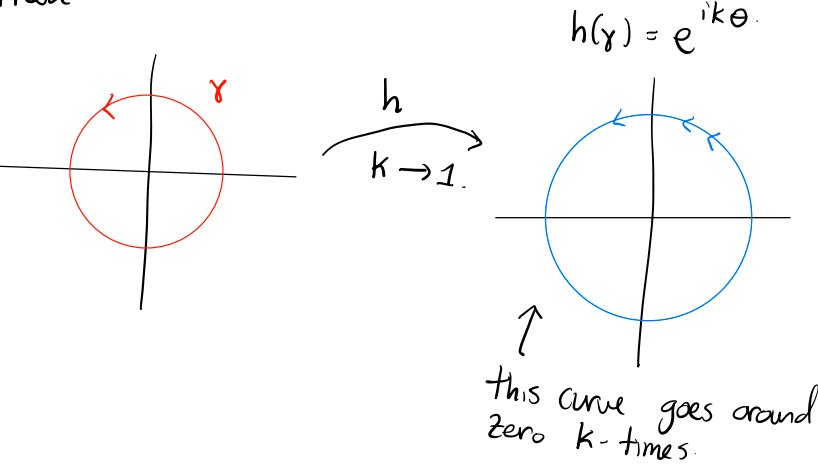
\includegraphics[width=0.75\textwidth]{LECTURE_13/gamma.png}
        \caption{The curve $\gamma$}
    \end{figure}

    \textbf{Step 1:} find $h'(z)/h(z)dz$:
    \begin{align*}
        \frac{h'(z)}{h(z)} & = d\log h(z) \text{ By definition}                                                                     \\
                           & = \underbrace{d\log|h|}_{\text{change in }|h(z)|} + \underbrace{id\theta}_{\text{change in }\arg h(z)} \\
                           & = dr + id\theta
    \end{align*}
    So:
    \begin{align*}
        \int_{\gamma} \frac{h'(z)}{h(z)}dz & = \int_{h(\gamma)} dr + id\theta                                          \\
                                           & = \log\frac{|h(\gamma(2\pi))|}{|h(\gamma(0))|} + i(\arg h(\gamma(2\pi)))k \\
                                           & = 0 _ i2\pi k
    \end{align*}
    Similarly if $h(z) = \frac{1}{z^k}$ then:
    \begin{figure}[H]
        \centering
        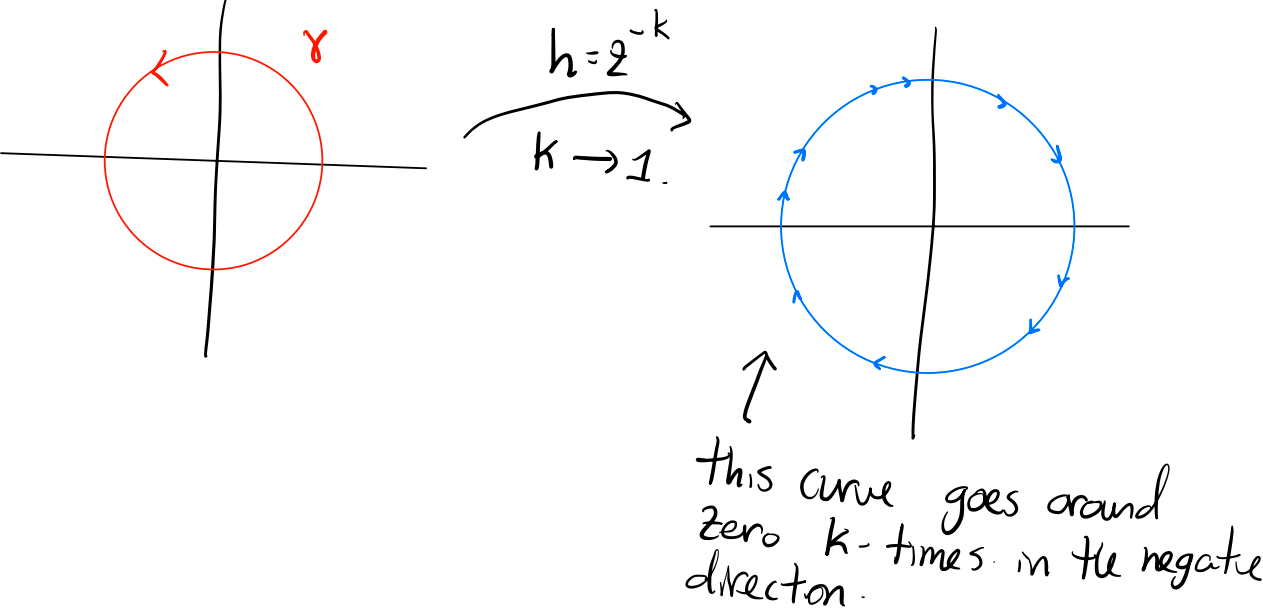
\includegraphics[width=0.75\textwidth]{LECTURE_13/gamma_rev.png}
        \caption{The reverse curve $\gamma$}
    \end{figure}

\end{example}

\begin{example}
    Find the number of zeroes of $f(z) = z^3 - 2z^2 + 4$ in the first quadrant
    \begin{figure}[H]
        \centering
        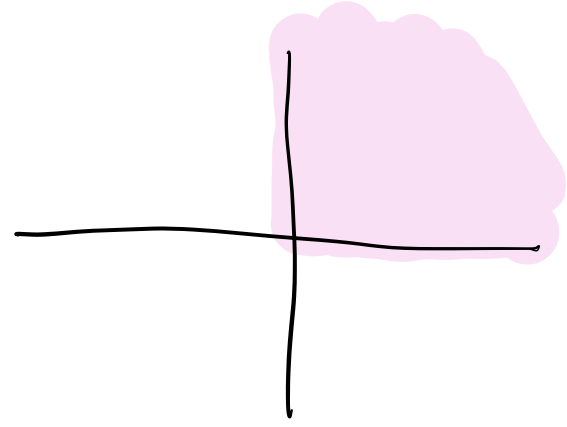
\includegraphics[width=0.75\textwidth]{LECTURE_13/first-quadrant.png}
        \caption{The first quadrant}
    \end{figure}

    \textbf{Solution:}
    \textbf{Step 1:} Consider the contour
    \begin{figure}[h]
        \centering
        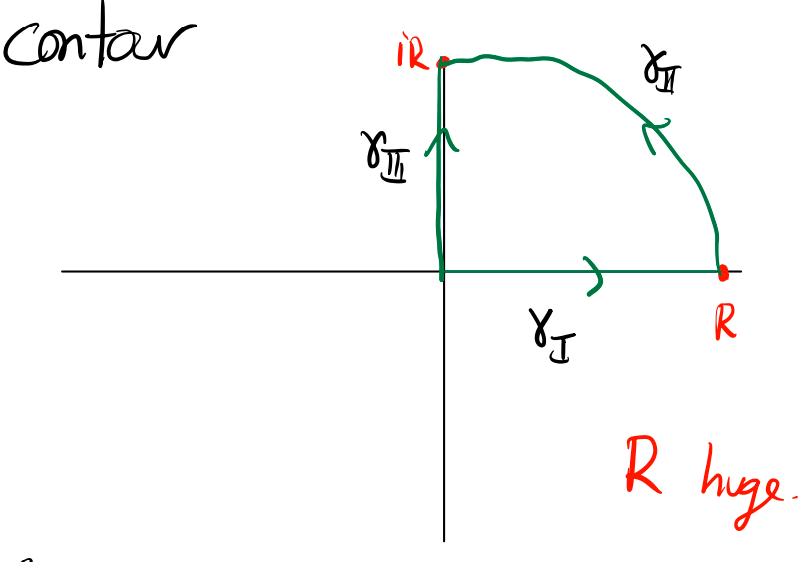
\includegraphics[width=0.75\textwidth]{LECTURE_13/first-quadrant-contour.png}
        \caption{The contour}
    \end{figure}
    \textbf{Step 2:} Find $\Delta \arg f(\gamma_k) \forall k$
    \begin{align*}
        \gamma_I & = x \quad t \in [0, R] \quad \rightarrow\quad f(\gamma_I) = t^3 - 2t^2 + 4
    \end{align*}
    This is a real function, so as long as $f(\gamma_I) \geq 0$ from $t = 0$ to $t = R$, then $\Delta \arg f(\gamma_I) = 0$. We know this function will have a minimum at $f'(t)$
    \begin{align*}
        f'                       & = 3t^2 - 4t = x(3x - 4)                                                                                                  \\
        \rightarrow f(0)         & = 4                                                                                                                      \\
        \rightarrow f(\frac{4}3) & = t^3 - 2t^2 + 4 = \frac{64}{27} - \frac{32}{9} + 4 = \frac{64}{27} - \frac{96}{27} + \frac{108}{27} = \frac{76}{27} > 0
    \end{align*}
    So $\Delta \arg f(\gamma_I) = 0$.
    \begin{align*}
        \gamma_{II}    & = Re^{i\theta}\quad \theta \in [0, \pi/2]                                             \\
        f(\gamma_{II}) & = R^3e^{3i\theta} - 2R^2e^{2i\theta} + 4                                              \\
                       & = R^3e^{3i\theta}\left(1 - \frac{2}{R}e^{i\theta} + \frac{4}{R^3}e^{-3i\theta}\right) \\
                       & \text{As } R \to \infty                                                               \\
                       & = R^3e^{3i\theta}
    \end{align*}
    $R$ is the magnitude of the function, complex exponential function gives the argument of the function.
    \begin{align*}
        e^{ig(\theta)} \rightarrow g(\theta) = \arg f(\gamma_{II}) = 3\theta
    \end{align*}
    Because $\theta \in [0, \pi/2]$ then $\Delta \arg f(\gamma_{II}) = 3\pi/2$.
    \begin{align*}
        \gamma_{III}    & = iy \quad \rightarrow\quad t \in [0, R] \\
        f(\gamma_{III}) & = iy^3 + 2y^2 + 4                        \\
    \end{align*}
    We know the argument of a function is given by $\tan^{-1}(\frac{\Im(f)}{\Re(f)})$
    \begin{align*}
        \arg f(\gamma_{III})_1 & = 0 \quad \text{because } f(\gamma_{III}(0)) = 4 \\
    \end{align*}
    Because the function begins on the real axis when $t = 0$, the argument is $0$.
    \begin{align*}
        \arg f(\gamma_{III})_2                 & =\lim_{y= R\to \infty} \tan^{-1}\left(\frac{y^3}{2y^2 + 4}\right) \\
                                               & = tan^{-1}(\inf) = \frac{\pi}2                                    \\
        \therefore \Delta \arg f(\gamma_{III}) & = \frac{\pi}2
    \end{align*}
    So all together:
    \begin{align*}
        \Delta \arg f(\gamma) & = \Delta \arg f(\gamma_I) + \Delta \arg f(\gamma_{II}) + \Delta \arg f(\gamma_{III}) \\
                              & = 0 + \frac{3\pi}2 + \frac{\pi}2 = 2\pi
    \end{align*}
    We notice that $f$ has no poles in the first quadrant, so by the argument principle:
    \begin{align*}
        \frac{1}{2\pi}\left\{\begin{aligned}
                                  & \text{change in } \arg h(z)            \\
                                  & \text{as } z \text{ traverses } \gamma
                             \end{aligned}\right\} + \left\{\begin{aligned}
                                                                 & \text{no. of poles of } h \\
                                                                 & \text{inside } \gamma
                                                            \end{aligned}\right\} & = \left\{\begin{aligned}
                                                                                                  & \text{no. of zeros of } h \\
                                                                                                  & \text{inside } \gamma
                                                                                             \end{aligned}\right\} \\
        \frac{1}{2\pi}\Delta \arg f(\gamma)            & = \frac{1}{2\pi}(\frac{3\pi}2 + \frac{\pi}2)                     \\
        1                                              & = \text{no. of zeroes of } f \text{ in the first quadrant}
    \end{align*}

\end{example}

\chapter{Homework 6: I Like MAT389!}

\chapter{Lecture 14: Rouché's Thm. \& Fundamental Thm. of Algebra}

\section{Last Time: Counting zeroes and poles of analytic functions}

\begin{proposition}
    We say:
    \begin{itemize}
        \item[]
        \item $h$ analytic in $D$, except finite number of poles $z_1, \ldots, z_n$.
        \item $\gamma$ piecewise $C^1$ closed curve, positively oriented, inside$(\gamma) \subset D$ avoiding zeroes and poles of $h$.
    \end{itemize}
    Then
    \begin{align*}
        (A) \quad & \frac{1}{2\pi i} \int_{\gamma} \frac{h'(z)}{h(z)} \, dz = \text{\# of zeroes of $h$ inside $\gamma$} - \text{\# of poles of $h$ inside $\gamma$}. \\
        (B)\quad  & \text{Argument Principle}                                                                                                                         \\
                  & \frac{1}{2\pi i} \left\{\text{Total change in Arg}(h(z))_{\gamma} \text{ as } z \text{ traverses} \right\}                                        \\
                  & = \text{\# of zeroes of $h$ inside $\gamma$} - \text{\# of poles of $h$ inside $\gamma$}.
    \end{align*}

\end{proposition}

\begin{theorem}
    [Rouche's Theorem]
    Suppose $f, g$ are analytic on $D$, $\gamma$ a curve in $D$ (piecewise $C^1$, simple, closed).\\
    if $|f(z) + g(z)| < |f(z)| \quad \forall z \in \gamma$ then $f$ and $g$ have the same number of \underline{zeroes} inside($\gamma$) (counting multiplicities).
\end{theorem}

\begin{proof}
    Neither $f$ nor $g$ have zeroes on $\gamma$.\\
    Suppose $f,g$ have zeroes of multiplicity $k$ at $z_0$. Then (by definition of zero multiplicity):
    \begin{align*}
        \tilde{f} = \frac{f(z)}{(z-z_0)^k}, \quad \tilde{g} = \frac{g(z)}{(z-z_0)^k}
    \end{align*}
    are analytic on $D$ (even at $z_0$). And $\tilde{f(z_0)} \neq 0 \neq \tilde{g(z_0)}$, and
    \begin{align*}
        |\tilde{f}(z) + \tilde{g}(z)| < |\tilde{f}(z)| \quad \forall z \in \gamma
    \end{align*}
    So the number of zeroes of $\tilde{f}$ (or $\tilde{g}$) inside $\gamma$ is
    \begin{align}
        \text{\#zeroes}(f)     & = \text{\#zeroes}((z-z_0)^k) + \text{\#zeroes}(\tilde{f}) = k + \text{\#zeroes}(\tilde{f}) \\
        \text{\#zeroes}(f) - k & = \text{\#zeroes}(\tilde{f})                                                               \\
        \text{\#zeroes}(g) - k & = \text{\#zeroes}(\tilde{g})
    \end{align}
    % \begin{align*}
    %     \text{\#zeroes}(\tilde{f} - \frac{k}{(z-z_0)^k}) = \text{\#zeroes}(f) - k  = \text{\#zeroes}(\tilde{g}) = \text{\#zeroes}(\tilde{g} - \frac{k}{(z-z_0)^k}) - k
    % \end{align*}
    % Because:
    % \begin{align*}
    %     (f) - k                         & = 0 \\
    %     \tilde{f} - \frac{k}{(z-z_0)^k} & = 0
    % \end{align*}
    So the number of zeroes of $\tilde{f}$ (or $\tilde{g}$) inside $\gamma$ is the number of zeroes of $f$ minus $k$
    So it suffices to assume $f,g$ have no common zeroes with $\gamma$.\\
    Also, if $\tilde{f}(z_0) = 0 = \tilde{g}(z_0)$ then $|f(z_0) + g(z_0)| < |f(z_0)|$ is impossible anyways.\\
\end{proof}

\begin{example}
    Consider $\frac{g}{f}$ Which has zeroes at zeroes of $g$ and poles at zeroes of $f$.\\
    \underline{and: } $|\frac{g}{f} + 1| = |\frac{g+f}{f}| < 1$ on $\gamma$.\\
    Consider the curve $\frac{g}{f} (\gamma)$
    \begin{figure}[h]
        \centering
        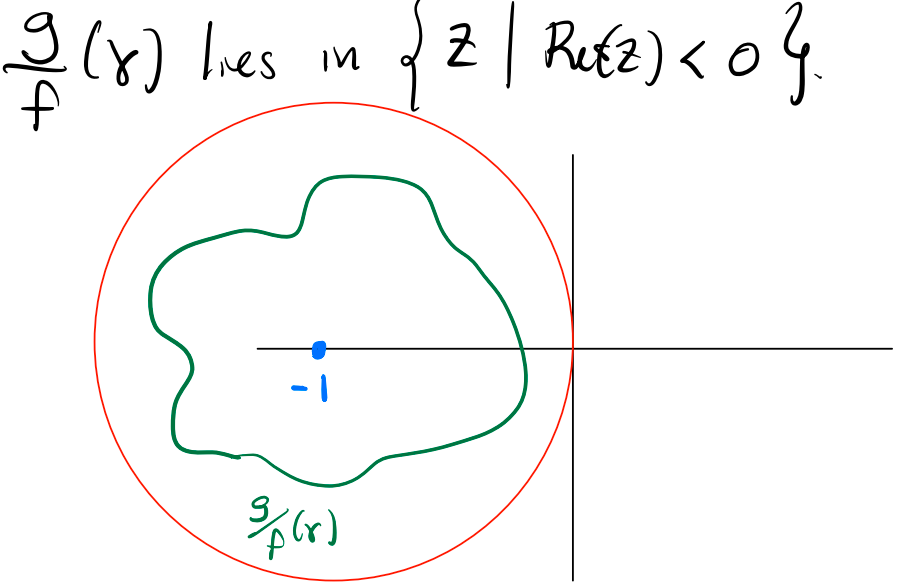
\includegraphics[width=0.8\textwidth]{LECTURE_14/gamma.png}
        \caption{Curve $\frac{g}{f} (\gamma)$}
    \end{figure}
    So, total change in argument of $\frac{g}{f}$ on $\gamma$ is \underline{zero}.\\
    So by the Argument Principle:
    \begin{align*}
        \text{\#zeroes}(\frac{g}{f}) = \text{\#poles}(\frac{g}{f}) = \text{\#zeroes}(f) = \text{\#poles}(g)
    \end{align*}

\end{example}

\begin{example}
    Show that all zeroes of the polynomial $p(z) = 3z^3 - 2z^2 + 2iz -8$ lie in the annulus $1 < |z| < 2$.\\
\end{example}

\begin{proof}
    \textbf{We apply Rouche's Theorem:}
    \textbf{Step 1:} Show that $p(z)$ has no zeroes inside $|z| = 1$.\\
    Consider the claim:
    \begin{align*}
        |p(z) + 8| < |8| \quad \forall z \in |z| = 1
    \end{align*}
    Let's show that it's true:

    \begin{align*}
        |p(z) + 8| & = |3z^3 - 2z^2 + 2iz|       \\
                   & \leq 3|z|^3 + 2|z|^2 + 2|z| \\
                   & = 3 + 2 + 2 = 7 < 8
    \end{align*}
    And therefore, the number of zeroes of $p$ in $|z| \leq 1$ is equal to the number of zeroes of 8, which is 0.\\
    \textbf{Step 2:} We expect an order 3 polynomial to have 3 zeroes, because there are none inside $|z| = 1$ we expect all 3 to be in $1 < |z| < 2$.\\

    Consider:
    \begin{align*}
        f(z)          & = -3z^3                                                                 \\
        |p(z) + f(z)| & < |f(z)| \text{ on } |z| = 2                                            \\
        |p(z) + f(z)| & = |-2z^2 + 2iz - 8|                                                     \\
                      & \leq 2|z|^2 + 2|z| + 8 = 2(4) + 2(2) + 8 = 20 < 3 \cdot 8 = 24 = |f(z)|
    \end{align*}

    So $p(z)$ has 3 zeroes in $1 < |z| < 2$ by Rouche's Theorem.\\
\end{proof}

\begin{theorem}
    [The Fundamental Theorem of Algebra]
    If you have a polynomial $p(z) = a_n z^n + a_{n-1} z^{n-1} + \ldots + a_1 z + a_0$ with $a_n \neq 0$ and $a_n, z \in \mathbb{C}$ then $p(z)$ has exactly $n$ zeroes in $\mathbb{C}$ (counting multiplicities).
\end{theorem}

\begin{proof}
    Let's compare $p(z)$ with $z^n$ on $|z| = R$ for $R$ large enough.\\
    \begin{align*}
        |p(z) - z^n| & \leq n\max_{0 \leq i \leq n - 1} |a_i||z|^i        \\
                     & = n\max_{|z| = R}^{n-1} |a_i| R^i \leq R^n = |z|^n
    \end{align*}
    So:
    \begin{align*}
        |p(z) - z^n| & < |z^n| \quad \forall |z| = R \quad \text{ for } R \text{ large enough}
    \end{align*}
    \underline{Rouche's} Theorem implies that $p(z)$ and $z^n$ have the same number of zeroes in $|z| < R$ for $R$ large enough.\\
\end{proof}


\chapter{Lecture 15: Properties of Analytic Functions}

\section{Maximum Modulus \& Mean Value}

\begin{theorem}
    [The Open Mapping Theorem]
    if $f$ is analytic on a Domain $D$, then either:
    \begin{itemize}
        \item $f$ is constant
        \item $f(D) \subseteq D$ is open
    \end{itemize}
\end{theorem}

\begin{proof}
    Recall that if $\Re(f) =  0$, then $f$ is constant
    Suppose $f$ is analytic, but not constant.\\
    Let $w_0 = f(z_0)$\\
    Since $f$ is not constant, we choose $r > 0$ (small), such that $f(z) - w_0$ has no zero in the set of $0 < |z -z_0| < r$\\
    \textbf{\underline{Why?}: Since zeroes of analytic functions are isolated}

    Let $0 < \delta = \min_{z \in |z - z_0|  = r} |f (z) - w_0| > 0$\\
    if $|w - w_0| < \delta$, then on $|z - z_0|  = r$:
    \begin{align*}
        |(f (z) - w) - (f(z) - w_0)| = |w- w_0| < \delta \leq |f(z) - w_0|
    \end{align*}
    By Rouche's Theorem, $f(z) - w$ has the same number of zeroes in $|z - z_0| \leq r$ as $f(z) - w_0$  (in particular, at least 1)
    \begin{align*}
        \Rightarrow w \in f(D) \text{ so } & \forall w \,| \,|w - w_0| < \delta, \exists z \in D \, | \, f(z)  = w \\
                                           & \{|w - w_0| < \delta  \in f(D)\}
    \end{align*}
    So $f(D)$ is open
\end{proof}

\begin{definition}
    [Mapping]
    A function $f: D \to \mathbb{C}$ is said to be $m \to 1$ at $z_0 \in D$ if in the neighborhood around $z_0$ there are exactly $m$ points in the domain $z$ that map to the same point $w = f(z_0)$ in the codomain.
\end{definition}

\begin{corollary}

    if $f$ is a non-constant analytic function on $D$ and $f(z) - f(z_0)$ has a zero of order $m$ at $z_0$, then $f(z)$ is $m \to 1$ map near $z_0$, in particular, if $f'(z_0) = 0$, then $f$ is not $1 \to 1$ in any disc around $z_0$. Furthermore, any disc around $z_0$ contains $m$ points $z \neq z_0$ such that $f(z) = f(z_0)$
\end{corollary}

\begin{example}
    if $f(z) = z^2$, has a zero of order $2$ at $0$\\
    if $z \neq 0$, then $f(z) = f(-z)$, so $f$ is $2 \to 1$
\end{example}
\begin{figure}[H]
    \centering
    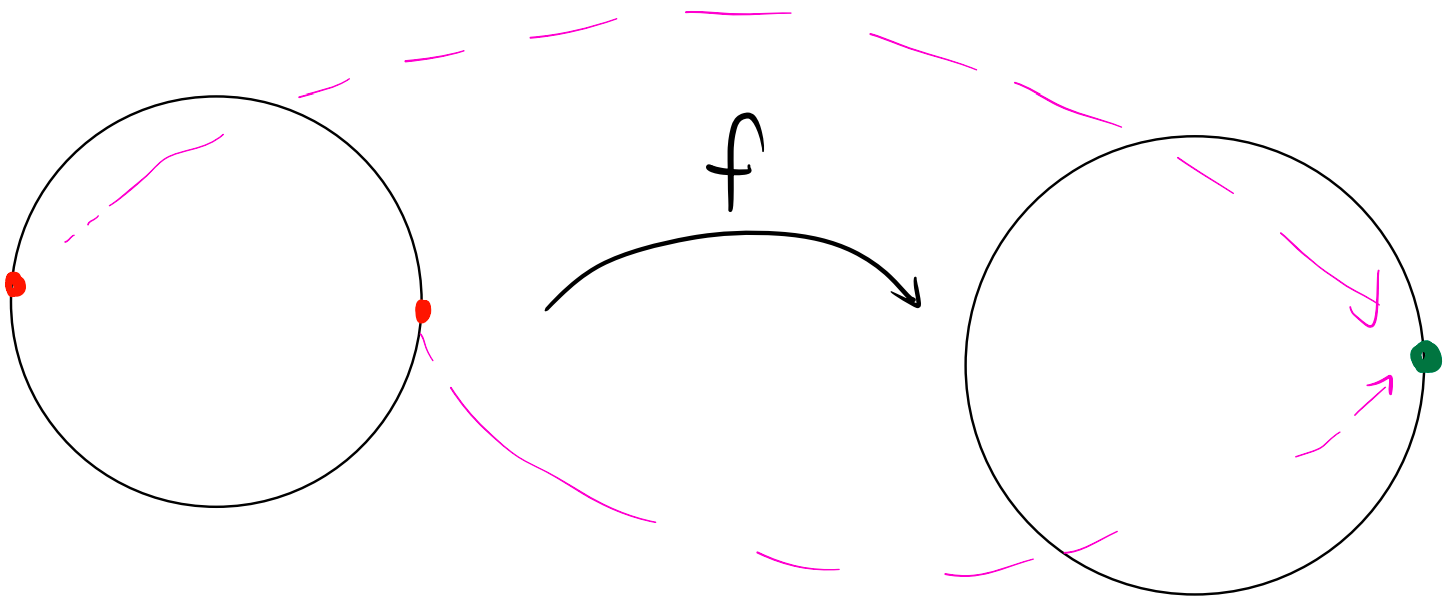
\includegraphics[width=0.5\textwidth]{LECTURE_15/max-mod.png}
    \caption{Mapping of $f(z) = z^2$}
\end{figure}
\begin{corollary}
    [Maximum Modulus Principle]
    if $f$ is a non-constant analytic function on the domain $D$, then $|f|$ has no local maximum.
\end{corollary}

\begin{remark}
    This may seem counterintuitive, but this is unique to complex functions. It is possible for a real differentiable function, $f$, to be non-constant and $|f|$ to have a local maximum.
\end{remark}

\begin{proof}
    Suppose $|f|$ has a local max at $z_0$, i.e.:
    $$|f(z)| \leq |f(z_0)| \quad \forall |z - z_0| \leq r$$
    For some $r > 0$, then $f(z_0)$ lies on the boundary of the set $\{f(z) \, | \, |z - z_0| < r\}$ because the maximum modulus in an open set is on the boundary, which is a contradiction to the open mapping theorem which states that $f(D)$ is open.
\end{proof}

\begin{theorem}
    [Schwartz Lemma]
    Suppose $f$ is analytic in a disc:
    \begin{align}
        \{|z| < 1\}, f(0) = 0 \text{ and } |f(z)| \leq 1 \forall |z| < 1 \\
    \end{align}
    \underline{Then} $|f(z)| \leq |z|\, \forall \, |z| < 1$, \underline{and}
    \begin{align}
        |f(\tilde{z})| & = |\tilde{z}| \text{ for some } z \neq 0, \text{ if and only if} \\
        f(z)           & = \lambda z \text{ for } \lambda \in \mathbb{C}, |\lambda| = 1
    \end{align}
\end{theorem}

\begin{proof}
    Say:
    \begin{align*}
        g(z) = \frac{f(z)}{z}, \quad |z| < 1
    \end{align*}
    Since $f(0) = 0$ we know $g(z) = \frac{f(z)}{z}$ is analytic for $|z| < 1$\\
    And on $|z| = r \quad (r < 1)$ we can write:
    \begin{align}
        |g(z)| \leq \frac{|f(z)|}{r} \leq \frac{1}{r}
    \end{align}
    So, by max modulus principle:
    \begin{align*}
        |g(z)| & < \frac{1}r \text{ on } \{|z| \leq r\} \\
    \end{align*}
    Because $\{g(z) \, : \, |z| = r \to 1\}$ needs to be open.\\
    Taking $r \to 1$, conclude
    \begin{align*}
        |g(z)| \leq \frac{|f(z)|}{|z|} \leq 1 \to f(z) \leq |z|
    \end{align*}
    We say $f(z) \leq |z|$ because $z \leq 1$, so we don't worry about openness.\\
    if $|f(z_0)| = |z_0|$, for some\\
    \textbf{Then} $|g(z)| = 1$, so $g(z)$ has an interior maximum. This means $g(z)$ is constant, so $f(z) = \lambda z$ for $|\lambda| = 1$
\end{proof}

\section{Mean-Value Property}
\begin{theorem}
    Suppose \( f = u + iv \) is analytic on \( \{ |z - z_0| \leq r \} \). Then, for any \( s \leq r \),

    the average value of \( u \) and \( v \) on the circle \( |z - z_0| = s \) is given by:
    \[
        \begin{rcases}
            u(z_0) = \frac{1}{2\pi} \int_{0}^{2\pi} u(z_0 + se^{i\theta}) \, d\theta \\
            v(z_0) = \frac{1}{2\pi} \int_{0}^{2\pi} v(z_0 + se^{i\theta}) \, d\theta
        \end{rcases} = \text{Average value of } u \text{ or } v \text{ on the circle } |z - z_0| = s
    \]
\end{theorem}


\begin{proof}
    \textbf{Cauchy's Integral Formula} with $\gamma(\theta) = z_0 + se^{i\theta}$:
    \begin{align*}
        f(z_0)                                      & = \frac{1}{2\pi i} \int_{|z - z_0| = s} \frac{f(z)}{z - z_0}dz                                    \\
        \rightarrow z = z_0 + se^{i\theta} \quad dz & = ise^{i\theta}d\theta                                                                            \\
        f(z_0)                                      & = \frac{1}{2\pi i} \int_{0}^{2\pi} \frac{f(z_0 + se^{i\theta})}{se^{i\theta}}ise^{i\theta}d\theta \\
    \end{align*}
    Now we take the real and imaginary parts of the above equation to get the average value of \( u \) and \( v \) on the circle \( |z - z_0| = s \).

\end{proof}

\section{Fractional Linear Transformations}

\begin{definition}
    [Fractional Linear Transformation]
    A FLT is a rational function of the form:
    \begin{align*}
        T(z) = \frac{az + b}{cz + d} \quad a,b,c,d \in \mathbb{C}, ad - bc \neq 0
    \end{align*}
\end{definition}

\begin{remark}
    Note: if $ad = bc$, then:
    \begin{align*}
        T'(z) = \frac{a (cz + d) - (az + b)c}{(cz + d)^2} = \frac{ad - bc}{(cz + d)^2} = 0
    \end{align*}
    So $T(z)$ is constant, and we're not interested in constant functions
\end{remark}

\begin{claim}
    $T$ is $1 \to 1$\\
    If $T(z_1) = T(z_2) \implies z_1 = z_2$.
    \begin{proof}
        \begin{align*}
            \frac{az_1 + b}{cz_1 + d}         & = \frac{az_2 + b}{cz_2 + d}    \\
            \iff acz_1^2 + adz_1 + bcz_1 + bd & = acz_2^2 + adz_2 + bcz_2 + bd \\
            (ad - bc)z_1                      & = (ad - bc)z_2                 \\
            z_1                               & = z_2
        \end{align*}
    \end{proof}
\end{claim}

\begin{claim}
    [T has an inverse]
    \begin{align*}
        T^{-1}(z) = \frac{dz - b}{-cz + a}
    \end{align*}
    Which is also a FLT
    \begin{proof}
        \begin{align*}
            T(z)                  & = w                          \\
                                  & = \frac{az + b}{cz + d}      \\
            \rightarrow z         & = \frac{dw - b}{-cw + a}     \\
            \rightarrow T^{-1}(w) & = \frac{dw - b}{-cw + a} = z
        \end{align*}
    \end{proof}
\end{claim}

\begin{claim}
    [Composition of FLT]
    if $T_1, T_2$ are FLT, then $T_1 \circ T_2$ is also a FLT
    \begin{proof}
        \begin{align*}
            T_1(z)      & = \frac{a_1z + b_1}{c_1z + d_1}                                                             \\
            T_2(z)      & = \frac{a_2z + b_2}{c_2z + d_2}                                                             \\
            T_1(T_2(z)) & = \frac{a_1(\frac{a_2z + b_2}{c_2z + d_2}) + b_1}{c_1(\frac{a_2z + b_2}{c_2z + d_2}) + d_1} \\
                        & = \frac{(a_1a_2z + a_1b_2 + b_1c_2z + b_1d_2)}{(c_1a_2z + c_1b_2 + d_1c_2z + d_1d_2)}       \\
                        & = \frac{(a_1a_2z + b_1b_2)}{(c_1a_2z + d_1b_2)}                                             \\
                        & = \frac{a_1a_2z + b_1b_2}{c_1a_2z + d_1b_2}                                                 \\
        \end{align*}
    \end{proof}
\end{claim}

\subsection{Matrix Representation of FLT}

\begin{theorem}
    Given $T(z) = \frac{az + b}{cz + d}$, we can represent $T$ as a matrix:
    $$A_T = \begin{pmatrix}
            a & b \\
            c & d
        \end{pmatrix}$$
    Where $A_T$ is a $2 \times 2$ matrix with determinant $ad - bc \neq 0$. So, $A_T$ is invertible
\end{theorem}

\begin{remark}
    Also:
    \begin{align*}
        A_{T_1 \circ T_2} = A_{T_1}A_{T_2}
    \end{align*}
    Note: if $\lambda \in \mathbb{C}, \lambda \neq 0$, then $A$ and $\lambda A$ give rise to the same FLT.
\end{remark}

\subsection{Point at Infinity}
\begin{definition}
    Recall that we can add the point at $\infty$ to $\mathbb{C}$ to get the $2$ sphere $S^2 = \mathbb{C} \cup \{\infty\}, \{x^2 + y^2 + z^2 = 1\}$
\end{definition}

\begin{figure}[H]
    \centering
    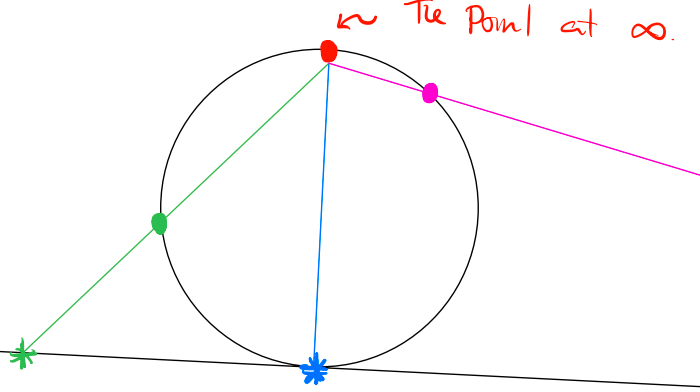
\includegraphics[width=0.5\textwidth]{LECTURE_15/s2.png}
    \caption{The Riemann Sphere}
\end{figure}

\begin{remark}
    An FLT should be be thought of in terms of how it moves points in $S^2$
\end{remark}

\begin{theorem}
    Consider $T(z) = \frac{a z + b}{c z + d}, (c \neq 0)$
    \begin{itemize}
        \item when $z = \frac{-d}{c}$, $T(z) = \infty$
        \item $\lim_{z \to \infty} T(z) = \frac{a + \frac{b}{z}}{c + \frac{d}{z}} = \frac{a}{c}$
    \end{itemize}
\end{theorem}

\begin{example}
    If $a, c = 1$, Then ($d \neq 0$):
    \begin{itemize}
        \item $T(0) = \frac{b}{d}$
        \item $T(\infty) = \frac{1}{d}$
        \item $T(\frac{-d}{c}) = \infty$
    \end{itemize}
\end{example}

\subsection{Fixed Points}

\begin{definition}
    [Fixed Points]
    A fixed point of $T(z) = z$ is a point $z_0$ such that $T(z_0) = z_0$
\end{definition}

\begin{lemma}
    An FLT has either $\leq 2$ fixed points or $\infty$ fixed points (it's the identity function)
\end{lemma}
\begin{proof}
    \begin{align*}
        T(z) & = \frac{az + b}{cz + d} = z \\
    \end{align*}
    So:
    \begin{align*}
        cz^2 + (d - a)z - b & = 0
    \end{align*}
    So, $z$ has at most $2$ solutions, unless $c = 0$, in which case $T(z) = z$ for all $z$
\end{proof}

\begin{proposition}
    A consequence of the above lemma is that if we're given:
    \begin{align*}
        \{z_1, z_2, z_3\} & \ \mathbb{C} \cup \{\infty\} = S^2  \quad \text{distinct}                  \\
                          & \{w_1, w_2, w_3\} \subset \mathbb{C} \cup \{\infty\} \quad \text{distinct} \\
    \end{align*}
    Then, there exists a unique FLT $T$ such that $T(z_i) = w_i,\quad i = 1, 2, 3$
\end{proposition}
\begin{proof}
    Consider:
    \begin{align*}
        L(z) = \frac{z - z_1}{z - z_3} \cdot \frac{z_2 - z_3}{z_2 - z_1}
    \end{align*}
    Then:
    \begin{itemize}
        \item $L(z_1) = 0$
        \item $L(z_2) = 1$
        \item $L(z_3) = \infty$
    \end{itemize}
    \textbf{Similarly}
    \begin{align*}
        S(w) = \frac{w - w_1}{w - w_3} \cdot \frac{w_2 - w_3}{w_2 - w_1}
    \end{align*}
    Then:
    \begin{itemize}
        \item $S(w_1) = 0$
        \item $S(w_2) = 1$
        \item $S(w_3) = \infty$
    \end{itemize}
    So, $S^{-1} \circ L$ is the FLT we're looking for. $T$ is unique since if $\tilde{T}$ maps $z_1 \to w_1$, then $T^{-1} \circ \tilde{T} (f)$ fixes $z_1, z_2, z_3$, so it must be the identity function.
    \begin{align*}
        \tilde{T} = T
    \end{align*}
\end{proof}

\chapter{Homework 7}

\begin{example}
    [Fisher, Section 2.5, Problem 10]

    Find the first four terms of the Laurent series of $f(z)=\frac z{\left(\sin(z)\right)^2}$ around $z_0=0$.That is, find an expansion of the form

    $$f(z)=\frac{a_{-1}}z+a_0+a_1z+a_2z^2+O(z^3)$$

    For $a_{-1},a_0,a_1,a_2\in\mathbb{C}.$

    \hrule
    \vspace{0.5cm}

    We know that:
    \begin{align*}
        \sin(z)                & =z-\frac{z^3}{3!}+\frac{z^5}{5!}-\frac{z^7}{7!}+\cdots      \\
        \left(\sin(z)\right)^2 & =z^2-\frac{2z^4}{3!}+\frac{2z^6}{5!}-\frac{2z^8}{7!}+\cdots
    \end{align*}
    Substituting that back into the original function, we get:
    \begin{align*}
        f(z) & =\frac z{\left(\sin(z)\right)^2}                                                    \\
             & =\frac z{z^2-\frac{2z^4}{3!}+\frac{2z^6}{5!}-\frac{2z^8}{7!}+\cdots}                \\
             & =\frac 1{z-\frac{2z^3}{3!}+\frac{2z^5}{5!}-\frac{2z^7}{7!}+\cdots}                  \\
             & =\frac 1z\cdot\frac 1{1-\frac{2z^2}{3!}+\frac{2z^4}{5!}-\frac{2z^6}{7!}+\cdots}     \\
             & =\frac 1z\cdot\left(1+\frac{2z^2}{3!}+\frac{2z^4}{5!}+\frac{2z^6}{7!}+\cdots\right) \\
             & =\frac 1z+\frac{2z}{3!}+\frac{2z^3}{5!}+\frac{2z^5}{7!}+\cdots                      \\
             & =\frac 1z+\frac 2{3!}z+\frac 2{5!}z^3+\frac 2{7!}z^5+\cdots                         \\
             & = \frac 1z + 0 + \frac 1{3}z + 0\cdot z^2 + O(z^3)
    \end{align*}

    Therefore, the first four terms of the Laurent series of $f(z)=\frac z{\left(\sin(z)\right)^2}$ around $z_0=0$ are:
    \begin{align*}
        a_{-1} & =1 \quad a_0=0 \quad a_1=\frac 1{3} \quad a_2=0
    \end{align*}
\end{example}


\begin{example}
    [Fisher, Section 2.5, Problem 12]

    Find the first four terms of the Laurent series of $f(z)=\frac1{e^z-1}$ around $z_0=0.$ That is,
    $$f(z)=\frac{a_{-1}}z+a_0+a_1z+a_2z^2+O(z^3)$$

    for $a_{-1},a_0,a_1,a_2\in\mathbb{C}.$

    \hrule
    \vspace{0.5cm}

    We know that:
    \begin{align*}
        e^z   & =1+z+\frac{z^2}{2}+\frac{z^3}{3!}+ \frac{z^4}{4!}+\cdots \\
        e^z-1 & =z+\frac{z^2}{2}+\frac{z^3}{3!}+ \frac{z^4}{4!}+\cdots
    \end{align*}
    Substituting that back into the original function, we get:
    \begin{align*}
        f(z) & =\frac1{e^z-1}                                                           \\
             & =\frac1{z+\frac{z^2}{2}+\frac{z^3}{3!}+ \frac{z^4}{4!}+\cdots}           \\
             & =\frac1z\cdot\frac1{1+\frac{z}{2}+\frac{z^2}{3!}+ \frac{z^3}{4!}+\cdots} \\
    \end{align*}
    We can use the geometric series formula to simplify the above expression, we know that:
    $$\frac1{1-x}=1+x+x^2+x^3+\cdots$$
    Therefore, we can rewrite the denominator as:
    \begin{align*}
        \frac1{1+\frac{z}{2}+\frac{z^2}{3!}+ \frac{z^3}{4!}+\cdots} & =\frac1{1-\left(-\frac z{2}-\frac{z^2}{3!}- \frac{z^3}{4!}-\cdots\right)} \\
                                                                    & \approx \frac1{1-\left(-\frac z{2}\right)} \quad \text{for small } z      \\
                                                                    & \rightarrow w = -\frac{z}{2} \quad \text{so}                              \\
                                                                    & = 1 - \frac{z}{2} + (-\frac{z}{2})^2 + (-\frac{z}{2})^3 + \cdots          \\
                                                                    & = 1 - \frac{z}{2} + \frac{z^2}{4} - \frac{z^3}{8} + \cdots
    \end{align*}
    Substituting that back into the original function, we get:
    \begin{align*}
        f(z) & =\frac1z\cdot\left(1 - \frac{z}{2} + \frac{z^2}{4} - \frac{z^3}{8} + \cdots\right) \\
             & =\frac1z-\frac{1}{2}+\frac{z}{4}-\frac{z^2}{8}+\cdots
    \end{align*}
    Therefore the first four terms of the Laurent series of $f(z)=\frac1{e^z-1}$ around $z_0=0$ are:
    \begin{align*}
        a_{-1} & =1 \quad a_0=-\frac 12 \quad a_1=\frac 14 \quad a_2=-\frac 18
    \end{align*}
\end{example}

\begin{example}
    [Fisher, Section 2.6, Problem 9]

    Compute the integral

    $$\int_0^{2\pi}\frac{d\theta}{(2-\sin(\theta))^2}$$

    \hrule
    \vspace{0.5cm}
    From the theorem in lecture 10, we know that residues of a function $f(z) = \frac{H(z)}{(z - z_0)^m}$ at a pole $z_0$ are given by: $\text{Res}(f, z_0) = \lim_{z \to z_0} \frac{H(z)}{(z - z_0)^m} = c_{m-1}$, where $c_{m-1}$ is the coefficient of the $(z - z_0)^{m-1}$ term in the Laurent series of $f(z)$ around $z_0$. Therefore, we can find the residue of the integrand at $z=0$ by finding the coefficient of the $z^{-1}$ term in the Laurent series of the integrand around $z=0$.
    We know that $\sin(\theta)=\frac{e^{i\theta}-e^{-i\theta}}{2i}$, so:
    \begin{align*}
        (2 - \frac{e^{i\theta}-e^{-i\theta}}{2i})^2 & = (\frac{4i - e^{i\theta} + e^{-i\theta}}{2i})^2                                         \\
                                                    & \rightarrow z = e^{i\theta}                                                              \\
                                                    & = (\frac{4i - z + \frac{1}{z}}{2i} )^2                                                   \\
                                                    & = -\frac{-16 - 4iz + \frac{4i}{z} - 4iz + z^2 - 1 + \frac{4i}{z} - 1 + \frac{1}{z^2}}{4} \\
                                                    & = -\frac{-18 - 8iz + z^2 + \frac{1}{z^2} + \frac{8i}{z}}{4}                              \\
                                                    & = \frac{9}{2} +2iz - \frac{z^2}{4} - \frac{1}{4z^2} - \frac{2i}{z}
    \end{align*}
    We can also change the infinitesimal $d\theta$ to $dz$:
    \begin{align*}
        dz = i e^{i\theta} d\theta \\
        d\theta = \frac{dz}{iz}
    \end{align*}

    Therefore, the integral becomes:
    \begin{align*}
        \int_0^{2\pi}\frac{d\theta}{(2-\sin(\theta))^2} & = \oint_{|z|=1} \frac{dz}{iz(\frac{9}{2} +2iz - \frac{z^2}{4} - \frac{1}{4z^2} - \frac{2i}{z})}
    \end{align*}
    Now we can use the residue theorem to evaluate the integral. Now we want to find where the integrand is singular. We can do this by setting the denominator to zero and solving for $z$:
    \begin{align*}
        4z^2(\frac{9}{2} +2iz - \frac{z^2}{4} - \frac{1}{4z^2} - \frac{2i}{z}) & = 0 \\
        18z^2 + 8iz^3 - z^4 - 1 - 8iz                                          & = 0 \\
    \end{align*}
    We assume that the solution is of the form $(z^2 +Az + B)(z^2 + Cz + D)$, so we can expand the above equation to get:\\
    $z^4 + (A+C)z^3 + (AC+B+D)z^2 + (AD+BC)z + BD  = z^4 - 8iz^3 - 18z^2 + 8iz  + 1 = 0$

    This gives the system of equations:
    \begin{align*}
        A+C    & = -8i \\
        AC+B+D & = -18 \\
        AD+BC  & = 8i  \\
        BD     & = 1
    \end{align*}
    Let's guess that $B = D = -1$ Because this would satisfy the last equation and make the first and third equations equivalent.
    \begin{align*}
        A+C    & = -8i \\
        AC     & = -16 \\
        -A - C & = 8i  \\
    \end{align*}
    By inspection we can see that $A = C = -4i$, this allows us to factor the denominator as:
    \begin{align*}
        (z^2 - 4iz - 1)^2 & = 0
    \end{align*}
    We can use the quadratic formula to find the roots of the above equation:
    \begin{align*}
        z & = \frac{b\pm\sqrt{b^2-4ac}}{2a}              \\
        z & = \frac{-4i\pm\sqrt{(-4i)^2-4(1)(-1)}}{2(1)} \\
        z & = \frac{-4i\pm\sqrt{-16+4}}{2}               \\
        z & = \frac{-4i\pm\sqrt{-12}}{2}                 \\
        z & = i(2 \pm \sqrt{3})
    \end{align*}

    Our contour is the unit circle where $|z| = 1$, so we're only considering residues within the unit circle.
    \begin{align*}
        |z_1| = |i(2 + \sqrt{3})| = 2 + \sqrt{3} > 1 \\
        |z_2| = |i(2 - \sqrt{3})| = 2 - \sqrt{3} < 1
    \end{align*}
    Therefore, the only pole within the unit circle is $z_2 = i(2 - \sqrt{3})$, and it's a double pole. We can find the residue at $z_2$ by finding the coefficient of the $z^{-1}$ term in the Laurent series of the integrand around $z_2$.
    \begin{align*}
        f(z) & = \frac{1}{iz(\frac{9}{2} +2iz - \frac{z^2}{4} - \frac{1}{4z^2} - \frac{2i}{z})} \\
             & = \frac{4zi}{(z - i(2 + \sqrt{3}))^2(z - i(2 - \sqrt{3}))^2}
    \end{align*}

    Using the residue theorem that says:
    \begin{align*}
        \oint_C f(z)dz                                                           & = 2\pi i \sum_{k=1}^n \text{Res}(f, z_k) \\
        \oint_{|z|=1} \frac{4zi}{(z - i(2 + \sqrt{3}))^2(z - i(2 - \sqrt{3}))^2} & = 2\pi i \text{Res}(f, z_2)
    \end{align*}

    We can find the residue at $z_2$, at $m = 2$
    \begin{align*}
        \text{Res}(f,z_k) & = \frac{1}{(m - 1)!}\lim_{z \to z_k} \frac{d^{m-1}}{dz^{m-1}} \left( (z - z_k)^m f(z) \right) \\
                          & = \frac{1}{1!}\lim_{z \to z_2} \frac{d}{dz} \left( (z - z_2)^2 f(z) \right)                   \\
                          & = \lim_{z \to z_2} \frac{d}{dz} \left( \frac{4zi(z - z_2)^2}{(z - z_1)^2(z - z_2)^2} \right)  \\
                          & = \lim_{z \to z_2} \frac{d}{dz} \left( \frac{4zi}{(z - z_1)^2} \right)                        \\
                          & = \lim_{z \to z_2} \frac{4(z - z_1) - 8i}{(z - z_1)^3}                                        \\
                          & = \frac{4(i(2 - \sqrt{3}) - i(2 + \sqrt{3})) - 8i}{(i(2 - \sqrt{3}) - i(2 + \sqrt{3}))^3}     \\
                          & = \frac{4(-2\sqrt{3}i) - 8i}{(-2\sqrt{3}i)^3}                                                 \\
                          & = \frac{-8\sqrt{3}i - 8i}{8\cdot 3i\sqrt{3}}                                                  \\
                          & = \frac{-\sqrt{3} - 1}{3\sqrt{3}}                                                             \\
    \end{align*}

    Therefore, the integral is:

    \begin{align*}
        \int_0^{2\pi}\frac{d\theta}{(2-\sin(\theta))^2} & = \oint_{|z|=1} \frac{dz}{iz(\frac{9}{2} +2iz - \frac{z^2}{4} - \frac{1}{4z^2} - \frac{2i}{z})} \\
                                                        & = 2\pi i \text{Res}(f, z_2)                                                                     \\
                                                        & = 2\pi i \left( = \frac{-\sqrt{3} - 1}{3\sqrt{3}} \right)                                       \\
                                                        & = \frac{-2\pi}{3\sqrt{3}}i
    \end{align*}
    So in summary, the steps to solve the integral are:
    \begin{itemize}
        \item Recognize that integrals of the form $\int f(\sin(\theta), \cos(\theta)) d\theta$ can be solved by converting to complex form.
        \item Convert the integrand to complex form by using the identity $\sin(\theta) = \frac{e^{i\theta} - e^{-i\theta}}{2i}$.
        \item Perform a change of variables to convert the integral from $d\theta$ to $dz$ by using $z = e^{i\theta}, \, d\theta = \frac{dz}{iz}$.
        \item Also remember to change the limits of integration to $|z| = 1$.
        \item Next we realize that it's possible that within our contour, the integrand has singularities. So we must use either the residue theorem or the Cauchy integral formula to evaluate the integral.
        \item In order to use the residue theorem, or Cauchy Integral Theorem, we must find the singularities of the integrand. We do this by setting the denominator to zero and solving for $z$.
        \item We find that the integrand has a double pole at $z = i(2 - \sqrt{3})$.
        \item Because there's one pole within the unit circle, we could use the cauchy integral formula to evaluate the integral. However, we chose to use the residue theorem.
        \item There are multiple ways to solve for a residue, note that $m$ is the order of the pole.
        \item[] \begin{itemize}
                  \item We can use the formula $\text{Res}(f, z_0) = \lim_{z \to z_0} \frac{H(z)}{(z - z_0)^m} = c_{m-1}$, where $c_{m-1}$ is the coefficient of the $(z - z_0)^{m-1}$ term in the Laurent series of $f(z)$ around $z_0$.
                  \item We can also use the formula $\text{Res}(f,z_k) = \frac{1}{(m - 1)!}\lim_{z \to z_k} \frac{d^{m-1}}{dz^{m-1}} ((z - z_k)^m f(z))$
                  \item or we can just expand the integrand into a Laurent series \textbf{around the singularity (not zero)}, then find the coefficient of the $z^{m-1}$ term
              \end{itemize}
        \item After finding the residue, we can use the residue theorem to evaluate the integral: $\oint_C f(z)dz = 2\pi i \sum_{k=1}^n \text{Res}(f, z_k)$.
    \end{itemize}
\end{example}

\begin{example}
    [Fisher, Section 2.6, Problem 10]

    Compute the integral

    $$\int_0^{2\pi}\frac{d\theta}{(1+\beta\cos(\theta))^2}\quad\mathrm{for~}-1<\beta<1$$

    \hrule
    \vspace{0.5cm}

    We can convert the denominator to a complex form by using the identity $\cos(\theta) = \frac{e^{i\theta} + e^{-i\theta}}{2}$, so:

    \begin{align*}
        (1 + \beta\cos(\theta))^2               & = (1 + \frac{\beta}{2}(e^{i\theta} + e^{-i\theta}))^2                                            \\
                                                & \rightarrow z = e^{i\theta} \quad dz = i e^{i\theta} d\theta \rightarrow d\theta = \frac{dz}{iz} \\
                                                & = (1 + \frac{\beta}{2}(z + \frac{1}{z}))^2                                                       \\
        \frac{d\theta}{(1+\beta\cos(\theta))^2} & = \frac{dz}{iz(1 + \frac{\beta}{2}(z + \frac{1}{z}))^{2}}                                        \\
    \end{align*}
    The limits of integration can be converted as well:
    \begin{align*}
        \theta = 0    & \rightarrow z = e^{i0} = 1    \\
        \theta = 2\pi & \rightarrow z = e^{i2\pi} = 1
    \end{align*}
    The path that the integral is taken over is the unit circle, so $|z| = 1$. We can now substitute the limits of integration and the integrand into the integral:
    \begin{align*}
        \int_0^{2\pi}\frac{d\theta}{(1+\beta\cos(\theta))^2} & = \oint_{|z|=1} \frac{dz}{iz(1 + \frac{\beta}{2}(z + \frac{1}{z}))^{2}}
    \end{align*}

    We can now find the singularities of the integrand by setting the denominator to zero and solving for $z$:
    \begin{align*}
        iz(1 + \frac{\beta}{2}(z + \frac{1}{z}))^{2}                                                                   & = 0 \\
        (1 + \frac{\beta}{2}(z + \frac{1}{z}))^{2}                                                                     & = 0 \\
        (\beta (z + \frac{1}{z}) + \frac{\beta^2}{4}(z + \frac{1}{z})^2 + 1)                                           & = 0 \\
        \beta (z + z^{-1}) + \frac{\beta^2}{4}(z^2 + 2 + z^{-2}) + 1                                                   & = 0 \\
        z^2\left(\beta z + \beta z^{-1} + \frac{\beta^2}{4}z^2 + \frac{\beta^2}{2} + \frac{\beta^2}{4}z^{-2} +1\right) & = 0 \\
        \beta z^3 + \beta z + \frac{\beta^2}{4}z^4 + \frac{\beta^2}{2}z^2 + \frac{\beta^2}{4} + z^2                    & = 0 \\
        \frac{\beta^2}{4}z^4 + \beta z^3 + \frac{\beta^2}{2}z^2 + z^2 + \beta z + \frac{\beta^2}{4}                    & = 0 \\
        \frac{\beta^2}{4}z^4 + \beta z^3 + (\frac{\beta^2}{2} + 1)z^2 + \beta z + \frac{\beta^2}{4}                    & = 0 \\
    \end{align*}

    We guess that the solution is symmetric, that is, it can be decomposed into two identical quadratics, i.e. $(Az^2 + Bz + C)^2$:\\
    $A^2 z^4 + 2ABz^3 + (2CA + B^2) z^2 + 2BCz + C^2 = \frac{\beta^2}{4}z^4 + \beta z^3 + (\frac{\beta^2}{2} + 1)z^2 + \beta z + \frac{\beta^2}{4}$\\

    This gives the system of equations:
    \begin{align*}
        A^2         & =  \frac{\beta^2}{4}     \\
        2AB         & = \beta                  \\
        (2CA + B^2) & =(\frac{\beta^2}{2} + 1) \\
        2BC         & = \beta                  \\
        C^2         & = \frac{\beta^2}{4}
    \end{align*}
    Right away we know $C = \pm \frac{\beta}{2}$, and so by inspection we can see that:
    \begin{align*}
        A = C & = \frac{\beta}{2} \\
        B     & = 1
    \end{align*}
    Therefore, the denominator can be factored as:
    \begin{align*}
        \left(\frac{\beta}{2}z^2 + z + \frac{\beta}{2}\right)^2 & = 0 \\
    \end{align*}
    We can use the quadratic formula to find the roots of the above equation:
    \begin{align*}
        z   & = \frac{-b\pm\sqrt{b^2-4ac}}{2a}                                               \\
        z   & = \frac{-1\pm\sqrt{1-4(\frac{\beta}{2})(\frac{\beta}{2})}}{2(\frac{\beta}{2})} \\
        z   & = \frac{-1\pm\sqrt{1-\beta^2}}{\beta}                                          \\
        z_1 & = \frac{-1+\sqrt{1-\beta^2}}{\beta}                                            \\
        z_2 & = \frac{-1-\sqrt{1-\beta^2}}{\beta}
    \end{align*}
    Multiplying the simplifying factors back in $(\frac{iz}{z^2})$ gets us the factorization:
    \begin{align*}
        \frac{i}{z}(z - z_1)^2(z - z_2)^2
    \end{align*}
    Now we find which poles are within the unit circle:
    \begin{align*}
        |z_1| \rightarrow 0 \leq \left|\frac{-1+\sqrt{1-\beta^2}}{\beta}\right| \leq 1 \\
        |z_2| \rightarrow 1 \leq \left|\frac{-1-\sqrt{1-\beta^2}}{\beta}\right| \leq 2
    \end{align*}
    Therefore, the only pole within the unit circle is $z_1 = \frac{-1+\sqrt{1-\beta^2}}{\beta}$, and it's a double pole. We can now use the residue theorem to evaluate the integral. It says:
    \begin{align*}
        \oint_C f(z)dz                                  & = 2\pi i \sum_{k=1}^n \text{Res}(f, z_k) \\
        \oint_{|z|=1} \frac{z}{i(z - z_1)^2(z - z_2)^2} & = 2\pi i \text{Res}(f, z_1)
    \end{align*}
    Using the formula for the residue of a double pole:
    \begin{align*}
        \text{Res}(f,z_k)     & = \frac{1}{(m - 1)!}\lim_{z \to z_k} \frac{d^{m-1}}{dz^{m-1}} ((z - z_k)^m f(z))                          \\
        \text{Res}(f,z_1)     & = \frac{1}{1!}\lim_{z \to z_1} \frac{d}{dz} \left( (z - z_1)^2 f(z) \right)                               \\
        \text{Res}(f,z_1)     & = \lim_{z \to z_1} \frac{d}{dz} \left(\frac{z(z - z_1)^2}{i(z - z_1)^2(z - z_2)^2} \right)                \\
        \text{Res}(f,z_1)     & = \lim_{z \to z_1} \frac{d}{dz} \left(\frac{z}{i(z - z_2)^2} \right)                                      \\
        \text{Res}(f,z_1)     & = \lim_{z \to z_1} \left(\frac{2i - i(z-z_2)}{(z - z_2)^3} \right)                                        \\
        \rightarrow z_1 - z_2 & = \frac{-1+\sqrt{1-\beta^2}}{\beta} - \frac{-1-\sqrt{1-\beta^2}}{\beta} = \frac{2\sqrt{1-\beta^2}}{\beta} \\
        \text{Res}(f,z_1)     & = \frac{2i - i(\frac{2\sqrt{1-\beta^2}}{\beta})}{(\frac{2\sqrt{1-\beta^2}}{\beta})^3}                     \\
        \text{Res}(f,z_1)     & = \frac{i\beta^3}{4\sqrt{1-\beta^2}^3} - \frac{i\beta^2}{4(1-\beta^2)}                                    \\
    \end{align*}
    Therefore, the integral is:
    \begin{align*}
        \int_0^{2\pi}\frac{d\theta}{(1+\beta\cos(\theta))^2} & = \oint_{|z|=1} \frac{dz}{iz(1 + \frac{\beta}{2}(z + \frac{1}{z}))^{2}}                        \\
                                                             & = 2\pi i \text{Res}(f, z_1)                                                                    \\
                                                             & = 2\pi i \left( \frac{i\beta^3}{4\sqrt{1-\beta^2}^3} - \frac{i\beta^2}{4(1-\beta^2)} \right)   \\
                                                             & = \frac{\pi}{2} \left( -\frac{\beta^3}{\sqrt{1-\beta^2}^3} + \frac{\beta^2}{1-\beta^2} \right)
    \end{align*}
\end{example}

\begin{example}
    [Fisher, Section 2.6, Problem 13]

    Compute the following integral

    $$\int_0^\infty\frac{x^\alpha}{x^2+3x+2}dx\quad\mathrm{for~}0<\alpha<1$$


    \hrule
    \vspace{0.5cm}

    We can convert the integral into a complex integral by realizing that $x = z$ and $x^\alpha = e^{\alpha\log(x)} = e^{\alpha\log(z)} = z^\alpha, \, dx = dz$.
    \begin{align*}
        \int_0^\infty\frac{x^\alpha}{x^2+3x+2}dx & = \int_0^\infty\frac{e^{\alpha\log(z)}}{z^2+3z+2}dz
    \end{align*}
    Because we've introduced a logarithm into the integral, we know we must choose a keyhole contour to evaluate the integral. Because the integral is evaluated over the positive real axis, we can choose the branch cut to be the positive real axis. This is because we know for a keyhole contour that:
    \begin{align*}
        \oint_{\text{Keyhole} = C} f(z)dz & = (\text{Path above the branch cut}) - (\text{Path below the branch cut}) \\
                                          & + (\text{Large arc}) - (\text{Small arc})                                 \\
    \end{align*}
    And as $R \rightarrow \infty$ and $R \rightarrow 0$, the integrals over the large and small arcs go to zero. So:
    \begin{align*}
        \oint_{\text{Keyhole} = C} f(z)dz & = (\text{Path above the branch cut}) - (\text{Path below the branch cut}) \\
                                          & = (1 - e^{2\pi i \alpha})\int_0^\infty f(z)dz
    \end{align*}
    We can now convert the integrand into a complex form by using the identity $\log(z) = \log|z| + i\arg(z)$:
    \begin{align*}
        \frac{e^{\alpha\log(z)}}{z^2+3z+2} & = \frac{e^{\alpha(\log|z| + i\arg(z))}}{z^2+3z+2}      \\
                                           & = \frac{e^{\alpha\log|z|}e^{i\alpha\arg(z)}}{z^2+3z+2} \\
                                           & = \frac{z^\alpha e^{i\alpha\arg(z)}}{z^2+3z+2}
    \end{align*}
    Now let's proceed with using the residue theorem.\\
    We can factor the denominator as:
    \begin{align*}
        z^2 + 3z + 2 & = (z + 2)(z + 1)
    \end{align*}
    This gives us the single poles at $z = -2$ and $z = -1$. We can now find the residues at these poles by using the formula, where $m = 1$:
    \begin{align*}
        \text{Res}(f, z_k) & = \frac{1}{(m - 1)!}\lim_{z \to z_k} \frac{d^{m-1}}{dz^{m-1}} ((z - z_k)^m f(z)) \\
        \text{Res}(f, -2)  & = \lim_{z \to -2} \frac{z^\alpha e^{i\alpha\arg(z)}}{(z + 1)}                    \\
                           & = \frac{(-2)^\alpha e^{i\alpha\arg(-2)}}{(-2 + 1)}                               \\
                           & = -(-2)^\alpha e^{i\alpha\pi}                                                    \\
        \rightarrow        & u^\alpha = e^{\alpha \log(u)}                                                    \\
                           & = -e^{\alpha \log(-2)} e^{i\alpha\pi}                                            \\
                           & = -e^{\alpha (\log(2) + i\arg(-2))} e^{i\alpha\pi}                               \\
                           & = -e^{\alpha (\log(2) + i\pi)} e^{i\alpha\pi}                                    \\
                           & = -2^\alpha e^{2i\alpha\pi}                                                      \\
        \text{Res}(f, -1)  & = \lim_{z \to -1} \frac{z^\alpha e^{i\alpha\arg(z)}}{(z + 2)}                    \\
                           & = \frac{(-1)^\alpha e^{i\alpha\arg(-1)}}{(-1 + 2)}                               \\
                           & = (-1)^\alpha e^{i\alpha\arg(-1)}                                                \\
                           & = (-1)^\alpha e^{i\alpha\pi}                                                     \\
                           & = e^{\alpha \log(-1)} e^{i\alpha\pi}                                             \\
                           & = e^{\alpha (\log(1) + i\arg(-1))} e^{i\alpha\pi}                                \\
                           & = e^{\alpha (0 + i\pi)} e^{i\alpha\pi}                                           \\
                           & = e^{i\alpha\pi} e^{i\alpha\pi}                                                  \\
                           & = e^{2i\alpha\pi}
    \end{align*}
    Therefore, the integral is:
    \begin{align*}
        \int_0^\infty\frac{x^\alpha}{x^2+3x+2}dx & = \frac{1}{1 - e^{2\pi i \alpha}}\oint_{\text{Keyhole} = C} f(z)dz                 \\
                                                 & = \frac{2\pi i}{1 - e^{2\pi i \alpha}}(\text{Res}(f, -2) + \text{Res}(f, -1))      \\
                                                 & = \frac{2\pi i}{1 - e^{2\pi i \alpha}}(-2^\alpha e^{2i\alpha\pi} +e^{2i\alpha\pi})
    \end{align*}

    So in summary, the steps to solve the integral are:
    \begin{enumerate}
        \item Recognize that the integral is over the positive real axis, and that the integrand has a logarithm in it.
        \item Because of the logarithm, we must choose a keyhole contour to evaluate the integral, and since the integral is over the positive real axis, we can choose the branch cut to be the positive real axis because $\oint_{\text{Keyhole} = C} f(z)dz = (\text{Path above the branch cut}) - (\text{Path below the branch cut}) = (1 - e^{2\pi i \alpha})\int_0^\infty f(z)dz$ as $R \rightarrow \infty$ and $R \rightarrow 0$.
        \item Convert the integrand into a complex form by using the identity $\log(z) = \log|z| + i\arg(z)$.
        \item Find the singularities of the integrand by setting the denominator to zero and solving for $z$.
        \item Find the residues at the poles by using the formula $\text{Res}(f, z_k) = \frac{1}{(m - 1)!}\lim_{z \to z_k} \frac{d^{m-1}}{dz^{m-1}} ((z - z_k)^m f(z))$.
        \item Use the residue theorem to evaluate the integral: $\oint_{\text{Keyhole} = C} f(z)dz = (\text{Path above the branch cut}) - (\text{Path below the branch cut}) = (1 - e^{2\pi i \alpha})\int_0^\infty f(z)dz$.
        \item After finding the residues, we can use the formula $\int_0^\infty\frac{x^\alpha}{x^2+3x+2}dx = \frac{2\pi i}{1 - e^{2\pi i \alpha}}(\text{Res}(f, -2) + \text{Res}(f, -1))$ to evaluate the integral.
    \end{enumerate}
\end{example}

\begin{example}
    [Fisher, Section 2.6 Problem 14]
    Compute the following integral
    $$\int_0^\infty\frac{\sqrt{x}}{x^2+2x+5}dx$$

    \hrule
    \vspace{0.5cm}

    We can convert the integral into a complex integral by realizing that $x = z$ and $dx = dz$.
    \begin{align*}
        \int_0^\infty\frac{\sqrt{x}}{x^2+2x+5}dx & = \int_0^\infty\frac{\sqrt{z}}{z^2+2z+5}dz
    \end{align*}
    Now we can find the singularities of the integrand by the quadratic formula:
    \begin{align*}
        z^2 + 2z + 5            & = 0                              \\
        z                       & = \frac{-b\pm\sqrt{b^2-4ac}}{2a} \\
        z                       & = \frac{-2\pm\sqrt{4-20}}{2}     \\
        z                       & = \frac{-2\pm\sqrt{-16}}{2}      \\
        z                       & = \frac{-2\pm4i}{2}              \\
        z                       & = -1\pm2i                        \\
        z_1                     & = -1+2i                          \\
        z_2                     & = -1-2i                          \\
        \therefore z^2 + 2z + 5 & = (z + 1 - 2i)(z + 1 + 2i)
    \end{align*}
    We can now find the residues at these poles by using the formula, where $m = 1$:
    \begin{align*}
        \text{Res}(f, z_k)   & = \frac{1}{(m - 1)!}\lim_{z \to z_k} \frac{d^{m-1}}{dz^{m-1}} ((z - z_k)^m f(z))                                                   \\
        \text{Res}(f, -1+2i) & = \lim_{z \to -1+2i} \frac{z^\frac{1}{2}}{(z + 1 + 2i)}                                                                            \\
                             & = \frac{(-1+2i)^{\frac{1}{2}}}{(-1+2i + 1 + 2i)}                                                                                   \\
                             & \rightarrow (-1+2i)^{\frac{1}{2}} \quad \text{De Moivre's Theorem}                                                                 \\
                             & \rightarrow z^n = r^n(\cos(\theta n) + i\sin(\theta n))                                                                            \\
                             & \rightarrow (-1+2i)^{\frac{1}{2}} = (\sqrt{5}(\cos(\pi - \tan^{-1}{\frac{2}1}) + i\sin(\pi - \tan^{-1}{\frac{2}1})))^{\frac{1}{2}} \\
                             & \rightarrow (-1+2i)^{\frac{1}{2}} \approx 5^\frac{1}{4}(\cos(\frac{2\pi}{3\times 2}) + i\sin(\frac{2\pi}{3\times 2}))              \\
                             & \rightarrow (-1+2i)^{\frac{1}{2}} \approx 5^\frac{1}{4}(\cos(\frac{\pi}{3}) + i\sin(\frac{\pi}{3}))                                \\
                             & \rightarrow (-1+2i)^{\frac{1}{2}} \approx 5^\frac{1}{4}(\frac{1}{2} + i\frac{\sqrt{3}}{2})                                         \\
                             & \rightarrow (-1+2i)^{\frac{1}{2}} \approx \frac{5^\frac{1}{4}}{2} + i\frac{5^\frac{1}{4}\sqrt{3}}{2}                               \\
                             & = \frac{\frac{5^\frac{1}{4}}{2} + i\frac{5^\frac{1}{4}\sqrt{3}}{2}}{4i}                                                            \\
                             & = -i\frac{5^\frac{1}{4}}8 - \frac{5^\frac{1}{4}\sqrt{3}}{8}                                                                        \\
    \end{align*}
    We can also find the residue at $z_2$:
    \begin{align*}
        \text{Res}(f, -1-2i) & = \lim_{z \to -1-2i} \frac{z^\frac{1}{2}}{(z + 1 - 2i)}                                                                            \\
                             & = \frac{(-1-2i)^{\frac{1}{2}}}{(-1-2i + 1 - 2i)}                                                                                   \\
                             & \rightarrow (-1-2i)^{\frac{1}{2}} \quad \text{De Moivre's Theorem}                                                                 \\
                             & \rightarrow (-1-2i)^{\frac{1}{2}} = (\sqrt{5}(\cos(\pi + \tan^{-1}{\frac{2}1}) + i\sin(\pi + \tan^{-1}{\frac{2}1})))^{\frac{1}{2}} \\
                             & \rightarrow (-1-2i)^{\frac{1}{2}} \approx 5^\frac{1}{4}(\cos(\frac{4\pi}{3\times 2}) + i\sin(\frac{4\pi}{3\times 2}))              \\
                             & \rightarrow (-1-2i)^{\frac{1}{2}} \approx 5^\frac{1}{4}(\cos(\frac{2\pi}{3}) + i\sin(\frac{2\pi}{3}))                              \\
                             & \rightarrow (-1-2i)^{\frac{1}{2}} \approx 5^\frac{1}{4}(-\frac{1}{2} + i\frac{\sqrt{3}}{2})                                        \\
                             & \rightarrow (-1-2i)^{\frac{1}{2}} \approx -\frac{5^\frac{1}{4}}{2} + i\frac{5^\frac{1}{4}\sqrt{3}}{2}                              \\
                             & = \frac{-\frac{5^\frac{1}{4}}{2} + i\frac{5^\frac{1}{4}\sqrt{3}}{2}}{4i}                                                           \\
                             & = i\frac{5^\frac{1}{4}}8 - \frac{5^\frac{1}{4}\sqrt{3}}{8}                                                                         \\
    \end{align*}

    Therefore, the integral is:
    \begin{align}
        \int_0^\infty\frac{\sqrt{x}}{x^2+2x+5}dx & =  \frac{1}{1 - e^{2\pi i \frac{1}{2}}}\oint_{\text{Keyhole} = C} f(z)dz                                                       \\
                                                 & = \frac{2\pi i}{1 - (-1)}(\text{Res}(f, -1+2i) + \text{Res}(f, -1-2i))                                                         \\
                                                 & = -\pi i(-i\frac{5^\frac{1}{4}}8 - \frac{5^\frac{1}{4}\sqrt{3}}{8} + i\frac{5^\frac{1}{4}}8 - \frac{5^\frac{1}{4}\sqrt{3}}{8}) \\
                                                 & = \frac{\pi i}{4}5^\frac{1}{4}\sqrt3
    \end{align}
\end{example}

\begin{example}
    [Fisher, Section 3.1, Problem 1]

    Determine the number of zeroes of $f(z) = z^2 - z + 1$ in the first quadrant (i.e. where $\Re(z) > 0, \Im(z) > 0$).

    \hrule
    \vspace{0.5cm}
    We can use the quadratic formula to find the zeroes of the function:
    \begin{align}
        z & = \frac{-b \pm \sqrt{b^2 - 4ac}}{2a}             \\
          & = \frac{-(-1) \pm \sqrt{(-1)^2 - 4(1)(1)}}{2(1)} \\
          & = \frac{1 \pm \sqrt{-3}}{2}
        z_1 = \frac{1}2 + i\sqrt{3}2                         \\
        z_2 = \frac{1}2 - i\sqrt{3}2                         \\
    \end{align}
    Only $z_1$ is in the first quadrant, so the answer is 1.
\end{example}

\begin{example}
    [Fisher, Section 3.1, Problem 3]

    Determine the number of zeroes of $f(z) = z^3 - 3z + 6$ in the first quadrant (i.e. where $\Re(z) > 0, \Im(z) > 0$).

    \hrule
    \vspace{0.5cm}

    We ca
\end{example}

\chapter{Lecture 16: Geometry of Fractional Linear Transformations}

\section{Lines \& Circles}

\begin{example}
    $T(z) = \frac{1}z$\\
    If $f(z) = |z-z_0|^2 - r^2 = 0$, then we can compute $f(T(z)$):
    \begin{align*}
        |z|^2 z\overline{z} - z\overline{z_0} - z_0\overline{z} + |z_0|^2 & = r^2                                                                            \\
        |z|^2 - 2\Re(z\overline{z_0}) + |z_0|^2                           & = r^2                                                                            \\\
        1 - 2\Re(z\overline{z_0}\frac{z}{|z|^2})                          & = \frac{r^2 - |z_0|^2}{|z|^2}                                                    \\
        \text{Then }                                                      & w = \frac{1}z \text{ satisfies}                                                  \\
        |w|^2(r^2 - |z_0|^2)                                              & = 1 - 2\Re(\frac{|w|^2}{w}\overline{z_0}) = 1 - 2\Re(\overline{w}\overline{z_0}) \\
        \rightarrow \Re(\overline{w}\overline{z_0})                       & = \Re(\overline{z_0}w)\end{align*}
    Which is just another circle, unless $z_0 = r$.
    \begin{align*}
        \text{If } r & = |z_0|, \text{ then}      \\
        \Re(wz_0)    & = \frac{1}2 \text{ A line}
    \end{align*}
    Therefore we see that $T(z) = \frac{1}z$ maps circles to lines if and only if $z = 0$ lies on the circle since $T(T(z)) = z$, we also see that $T$ takes lines to circles.
\end{example}

\begin{proposition}
    [Möbius Transformation (Lines \& Circles)]
    Given a circle: $f(z) = |z-z_0|^2 - r^2 = 0$, then $T(z) = \frac{1}{z - a}$ maps the circle to a line if and only if the edge of the circle passes through $a$ so that $|a - z_0| = r$. \\
    The equation of the line is $\Re(wz_0) = \frac{1}2$ where $w = \frac{1}{z - a}$.
\end{proposition}

\begin{figure}[H]
    \centering
    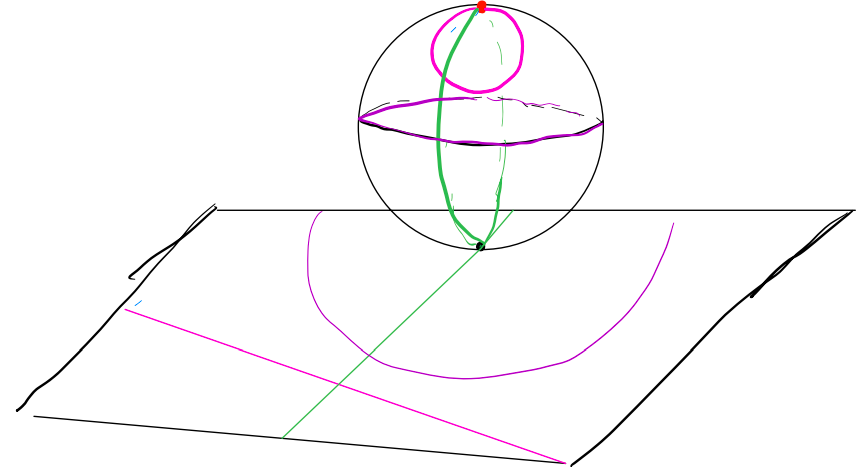
\includegraphics[width=0.5\textwidth]{LECTURE_16/circle-through-infty.png}
    \caption{Circle through $\infty$}
\end{figure}

\begin{lemma}
    If $T$ is a fractional linear transformation, then either $T$ is \underline{linear} or, these exist $T_1, T_3$ are \underline{linear} (i.e. $T_1(z) = a_1z + b_1, T_3(z) = a_3z + b_3$) such that if we take $T_2(z) = \frac{1}{z}$, then:
    \begin{align*}
        T = T_3 \circ T_2 \circ T_1
    \end{align*}
\end{lemma}

\begin{proof}
    $T= \frac{az + b}{cz + d}$, $T$ is linear if and only if $c = 0$, so we assume $c \neq 0$.\\
    \begin{align*}
        T & = \frac{1}{c} \left(\frac{bc - ad}{cz + d} + a\right)
    \end{align*}
    Then we define:
    \begin{align*}
        T_3(z) & = \frac{1}{c} (bc - ad)z + a \\
        T_1(z) & = cz + d
    \end{align*}
\end{proof}

\begin{corollary}
    A fractional linear transformation takes:
    \begin{align*}
        \left\{
        \begin{aligned}
             & \text{Circles or} \\
             & \text{Lines}
        \end{aligned}
        \right\}
         & \xrightarrow{T}
        \left\{
        \begin{aligned}
             & \text{Circles or} \\
             & \text{Lines}
        \end{aligned}
        \right\}
    \end{align*}
\end{corollary}

\begin{proof}
    If $T$ is linear, then $T$ takes lines to lines and circles to circles. If $T$ is not linear, then $T = T_3 \circ T_2 \circ T_1$ where $T_1, T_3$ are linear and $T_2(z) = \frac{1}{z}$ takes lines to circles/lines and circles to lines/circles.
\end{proof}

\section{Conformal Mapping}

\begin{proposition}
    Suppose $z_1(t)$ and $z_2(t)$ are curves in $\mathbb{C}$, (say for $t \in [-1, 1]$) and $z_1(0) = z_2(0) = z_0$. The tangent vector of the curves $z_j(t) = x_j(t) + iy_j(t), \quad j = 1, 2$ is given by:
    \begin{align*}
        z'_j(t) = x'_j(t) + iy'_j(t)
    \end{align*}
    The angle between $z_1, z_2$ at $(t = 0, z_0)$ is given by:
    \begin{align*}
        \theta =  \arg(z'_2(0))- \arg(z'_1(0))
    \end{align*}

    \begin{figure}[H]
        \centering
        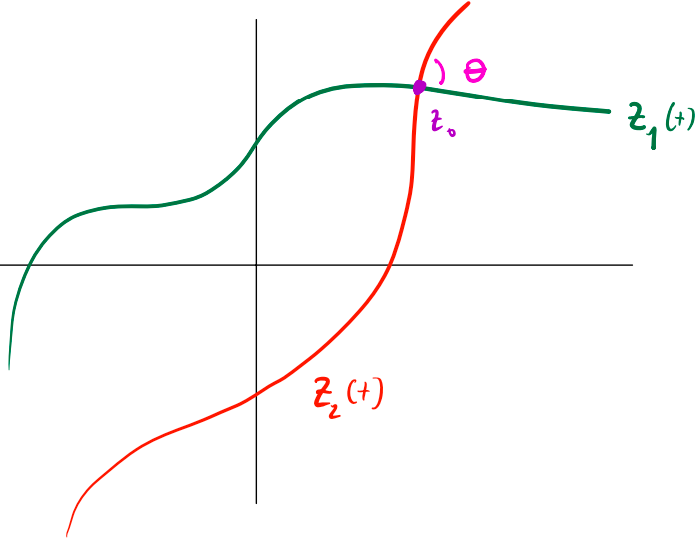
\includegraphics[width=0.5\textwidth]{LECTURE_16/graph.png}
        \caption{Angle between curves}
    \end{figure}

    Now suppose $f$ is an analytic function defined in $|z - z_0| < r$ such that $f'(z_0) \neq 0$. Then:
    \begin{align*}
        w_1(t) & = f(z_1(t)), \quad w_2(t) = f(z_2(t)) \text{ are curves in } \mathbb{C} \\
    \end{align*}

    \begin{figure}[H]
        \centering
        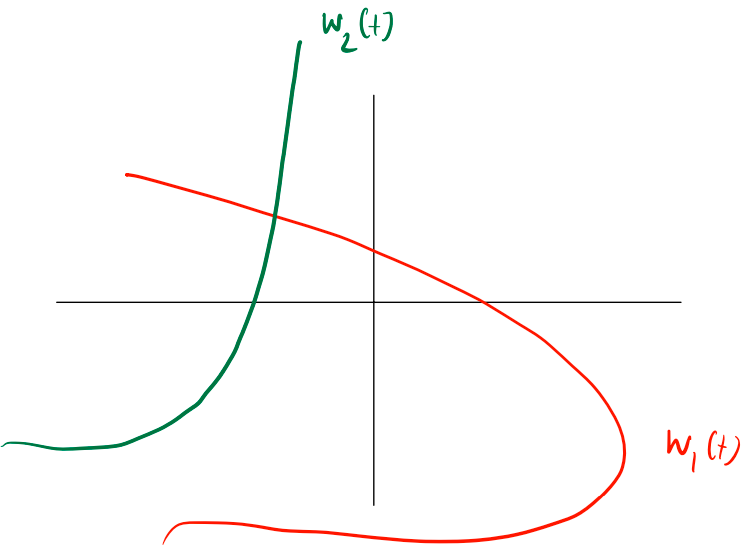
\includegraphics[width=0.5\textwidth]{LECTURE_16/graph2.png}
        \caption{Curves under $f$}
    \end{figure}

    The tangent vector to $w_j(t)$ at $t = 0$ is given by:
    \begin{align*}
        w'_j(0) = f'(z_0)z'_j(0)
    \end{align*}
    And the \underline{angle} between some $w_i, w_j$ is:
    \begin{align}
        \arg(w'_j(0)) = \arg(f'(z_0)) + \arg(z'_j(0)) \quad j = 1, 2
    \end{align}
    so
    \begin{align}
        \arg(w'_2(0)) - \arg(w'_1(0)) = \arg(z'_2(0)) - \arg(z'_1(0))
    \end{align}
    (This is because if $u = u_1\cdot u_2, \quad \arg(u) = \arg(u_1) + \arg(u_2)$)
    also
    \begin{align}
        |w'_j(0)| = |f'(z_0)||z'_j(0)| \quad j = 1,2
    \end{align}
\end{proposition}

\begin{definition}
    [Conformal Map]
    A conformal map $\phi : \mathbb{C} \to \mathbb{C}$ is a map such that
    \begin{enumerate}
        \item if $\gamma_1(t), \gamma_2(t)$ are two curves such that $\gamma_1(0) = \gamma_2(0)$ then
        \item[] Angle between $\gamma_1'(0)$ and $\gamma_2'(0)$ = Angle between $\phi(\gamma_1)'(0)$ and $\phi(\gamma_2)'(0)$
        \item[]
        \item The lengths of tangent vectors are \underline{scaled} by a positive constant
        \item[] $|\gamma_j'(0)|c = |\phi(\gamma_j)'(0)|$
    \end{enumerate}
    Essentially, a conformal map preserves angles, but not necessarily lengths.
\end{definition}

\begin{theorem}
    If $f$ is analytic near $z_0$, and $f'(z_0) \neq 0$, then $f$ is a conformal map near $z_0$.
\end{theorem}

\begin{example}
    [Map Projections]
    The mercator projection is conformal, so it preserves \underline{compass angles} and hence very useful for navigation.
\end{example}

\chapter{Lecture 17: Level Curves \& The Riemann Mapping Theorem}

\section{Level Curves}

\begin{claim}
    [Orthogonal Level Curves]
    Suppose $f = u + iv$ is an analytic function and some $f'(z_0) \neq 0$. Then the level curves of $u$ and $v$ centered around $z_0$ intersect orthogonally at $z_0 = x_0 + iy_0$.
    \begin{align*}
        \gamma_1 & = \{z : u(z) = u(z_0)\} \text{ the set of points in } \mathbb{C} \text{ where real part of } f \text{ is constant}      \\
        \gamma_2 & = \{z : v(z) = v(z_0)\} \text{ the set of points in } \mathbb{C} \text{ where imaginary part of } f \text{ is constant}
    \end{align*}
    This is because at $z_0$ is the only point shared between $\gamma_1$ and $\gamma_2$.
    \begin{figure}[H]
        \centering
        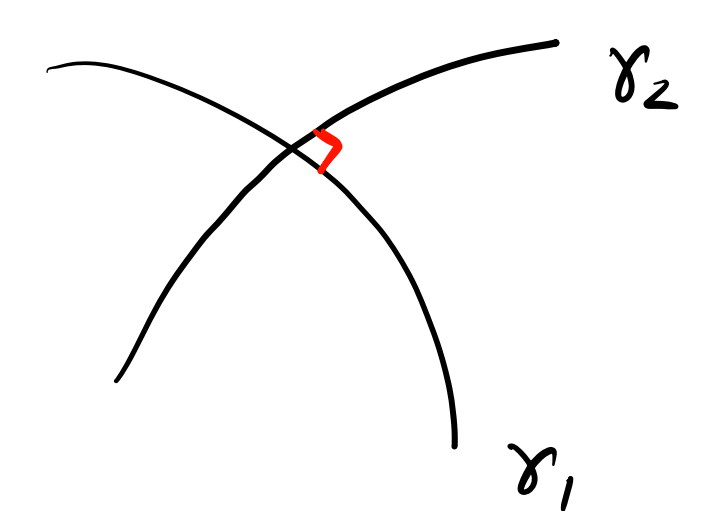
\includegraphics[width=0.5\textwidth]{LECTURE_17/graph.png}
        \caption{Level Curves}
    \end{figure}
\end{claim}

\begin{proof}
    $f$ is a conformal map and $\gamma_1, \gamma_2$ are curves in $\mathbb{C}$ such that $\gamma_1(0) = \gamma_2(0) = z_0$. So the angle between $\gamma_1, \gamma_2$ at $z_0$ is the same as the angle between $f(\gamma_1), f(\gamma_2)$ at $f(z_0)$.
    \begin{itemize}
        \item $f(\gamma_1) = \{w \in \mathbb{C} :\Re (w) = u(z_0)\}$
        \item[$\rightarrow$] $w = f(z)$ for each $z \in \gamma_1$
        \item[] We know for each $z \in \gamma_1$ that $u(z) = u(z_0)$
        \item[] Because $f^{-1}(w) = z$, we have $u(f^{-1}(w)) = u(z) = u(z_0) = \Re (w)$
        \item $f(\gamma_2) = \{w \in \mathbb{C} :\Im (w) = v(z_0)\}$
    \end{itemize}
    \begin{figure}[H]
        \centering
        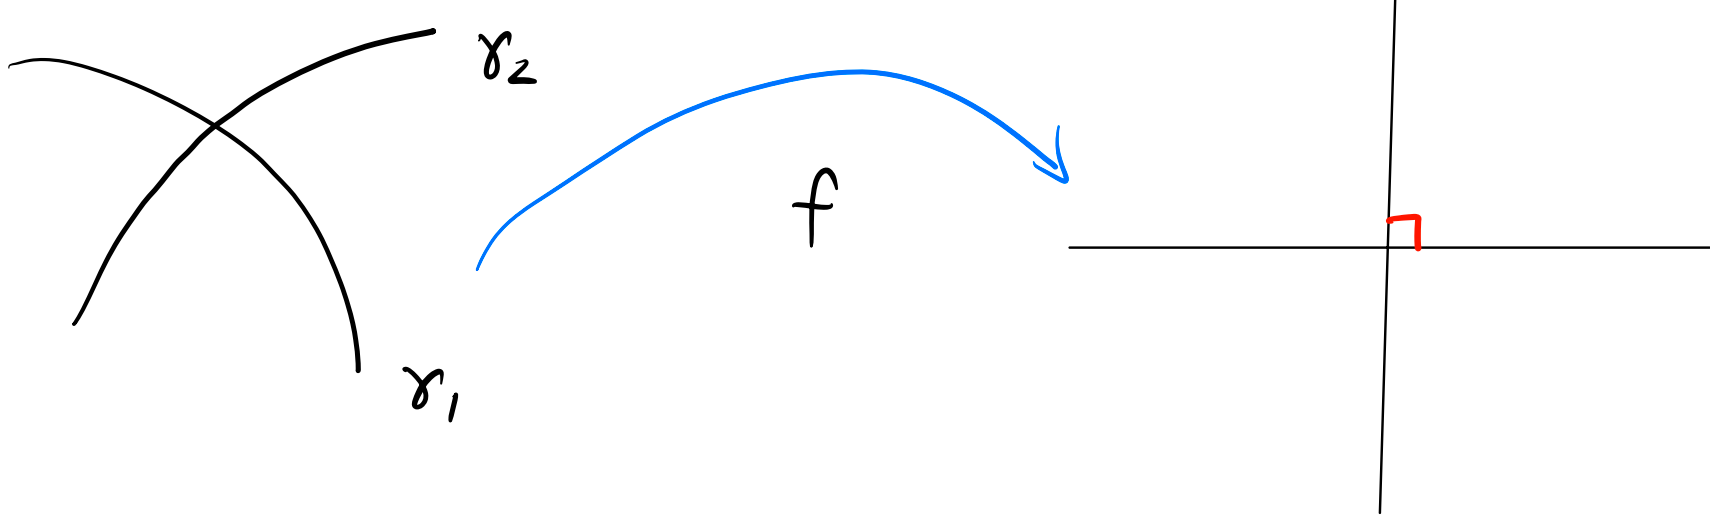
\includegraphics[width=0.5\textwidth]{LECTURE_17/conformal.png}
        \caption{Level Curves under $f$}
    \end{figure}
    Due to the fact that $nabla u \cdot \nabla v = 0$ at every point, this means $f(\gamma_1) = u(z_0)$ and $f(\gamma_2) = v(z_0)$ intersect orthogonally at $f(z_0)$, and thus $\gamma_1, \gamma_2$ intersect orthogonally at $z_0$.
\end{proof}

\begin{example}
    \begin{itemize}
        \item[(i)] $f(z) = e^z = \underbrace{e^x(\cos y)}_u + i\underbrace{e^x(\sin y)}_{v}$
    \end{itemize}
    \begin{figure}[H]
        \centering
        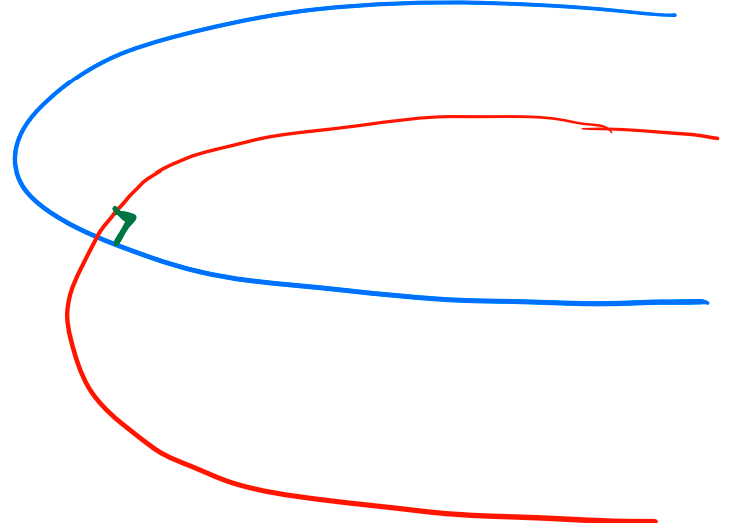
\includegraphics[width=0.5\textwidth]{LECTURE_17/graph1.png}
        \caption{Level Curves of $e^z$}
    \end{figure}
    Let's consider the level curves of $u$ and $v$.
    \begin{align*}
        \gamma_1    & = \{z \in \mathbb{C} : u(z) = u(z_0)\}                   \\
        e^x(\cos y) & = C_1 \quad \text{for some constant } C_1 \in \mathbb{R} \\
    \end{align*}
    If $C_1 = 0$ then:
    \begin{align*}
        e^x(\cos y) = 0 \implies \cos y = 0 \implies y = \frac{\pi}{2} + n\pi
    \end{align*}
    If $C_1 \neq 0$ then:
    \begin{align*}
        e^x(\cos y) = C_1 \implies e^x & = \frac{C_1}{\cos y} \quad \text{for } y \neq \frac{\pi}{2} + n\pi \\
        x                              & = \log \left(\frac{C_1}{\cos y}\right)
    \end{align*}
    So $\gamma_1$ is a set of $z = (x, y)$ such that $x = \log \left(\frac{C_1}{\cos y}\right)$ for $y \neq \frac{\pi}{2} + n\pi$.\\
    Similarly, $\gamma_2$ is a set of $z = (x, y)$ such that $x = \log \left(\frac{C_2}{\sin y}\right)$ for $y \neq n\pi$.\\
    Because $f'(z_0) = e^{z_0} \neq 0$, we can show that the level curves of $u$ and $v$ intersect orthogonally at any point $z_0$.
    \begin{align*}
        \nabla u & = \begin{pmatrix}
                         \frac{\partial u}{\partial x} \\ \frac{\partial u}{\partial y}
                     \end{pmatrix} = \begin{pmatrix}
                                         e^x\cos y \\ -e^x\sin y
                                     \end{pmatrix} \\
        \nabla v & = \begin{pmatrix}
                         \frac{\partial v}{\partial x} \\ \frac{\partial v}{\partial y}
                     \end{pmatrix} = \begin{pmatrix}
                                         e^x\sin y \\ e^x\cos y
                                     \end{pmatrix}
    \end{align*}
    Then we can use the dot product, which is $0$ iff the vectors are orthogonal.
    \begin{align*}
        \nabla u \cdot \nabla v = e^{x}\cos(y)e^{x}\sin(y) - e^{x}\cos(y)e^{x}\sin(y) = 0
    \end{align*}
\end{example}

\begin{example}
    \begin{itemize}
        \item[(ii)] $\text{Log} z = \underbrace{\log |z|}_u + i\underbrace{\text{Arg}(z)}_v$
    \end{itemize}
    \begin{figure}[H]
        \centering
        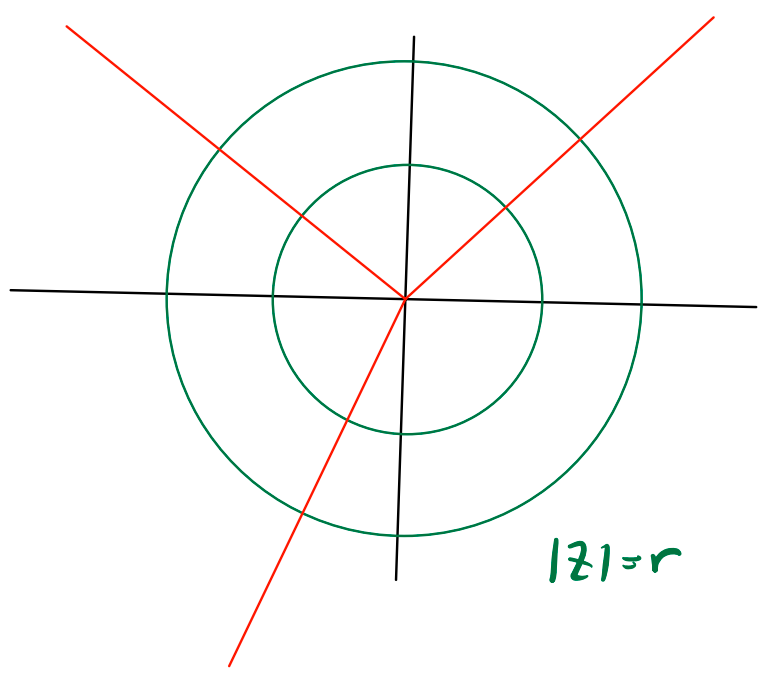
\includegraphics[width=0.5\textwidth]{LECTURE_17/graph2.png}
        \caption{Level Curves of $\text{Log} z$}
    \end{figure}
\end{example}

\section{The Riemann Mapping Theorem}

\begin{theorem}
    [Riemann Mapping Theorem]
    Suppose $D \subset \mathbb{C}$ is a simply connected domain such that $D \neq \mathbb{C}$. Let $p \in D$ be a point in $D$. Then there is a one-to-one analytic function $\phi$ such that:
    \begin{align*}
        \phi : D \to \{w \in \mathbb{C} : |w| < 1\}
    \end{align*}
    and $\phi(p) = 0$. $\phi$ is uniquely determined if we require $\phi'(p) > \mathbb{R}_{> 0}$.\\
    Basically, we can map any simply connected domain to the unit disk.
\end{theorem}

\begin{corollary}
    If $D_1, D_2$ are simply connected domains $D_1 \neq \mathbb{C} \neq D_2$, then $\exists \phi$ that's one-to-one and analytic such that:
    \begin{align*}
        \phi(D_1) = D_2
    \end{align*}
\end{corollary}

\begin{proof}
    $D_1 \xrightarrow{\phi_1} \{w \in \mathbb{C} : |w| < 1\}$ and $D_2 \xrightarrow{\phi_2} \{w \in \mathbb{C} : |w| < 1\}$.\\
    $\phi_2^{-1} \circ \phi_1$ is the desired map.
\end{proof}

\begin{figure}[H]
    \centering
    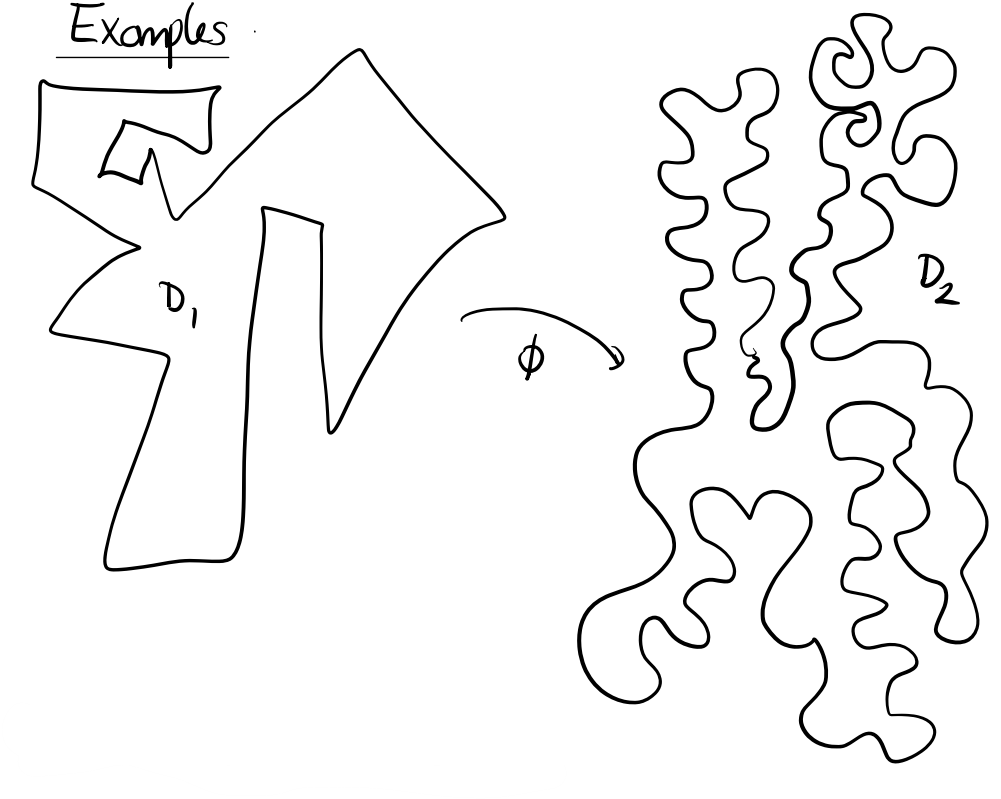
\includegraphics[width=0.5\textwidth]{LECTURE_17/graph3.png}
    \caption{Riemann Mapping Theorem}
\end{figure}
\begin{remark}
    This only proves the \underline{existence}! In general, it is not constructive!
\end{remark}

\section{Constructing Conformal Maps}

\begin{example}

    Mapping the unit disk to the upper half plane.\\
    \begin{align*}
        f = i\left(\frac{1 + z}{1 - z}\right)
    \end{align*}
\end{example}

\begin{figure}[H]
    \centering
    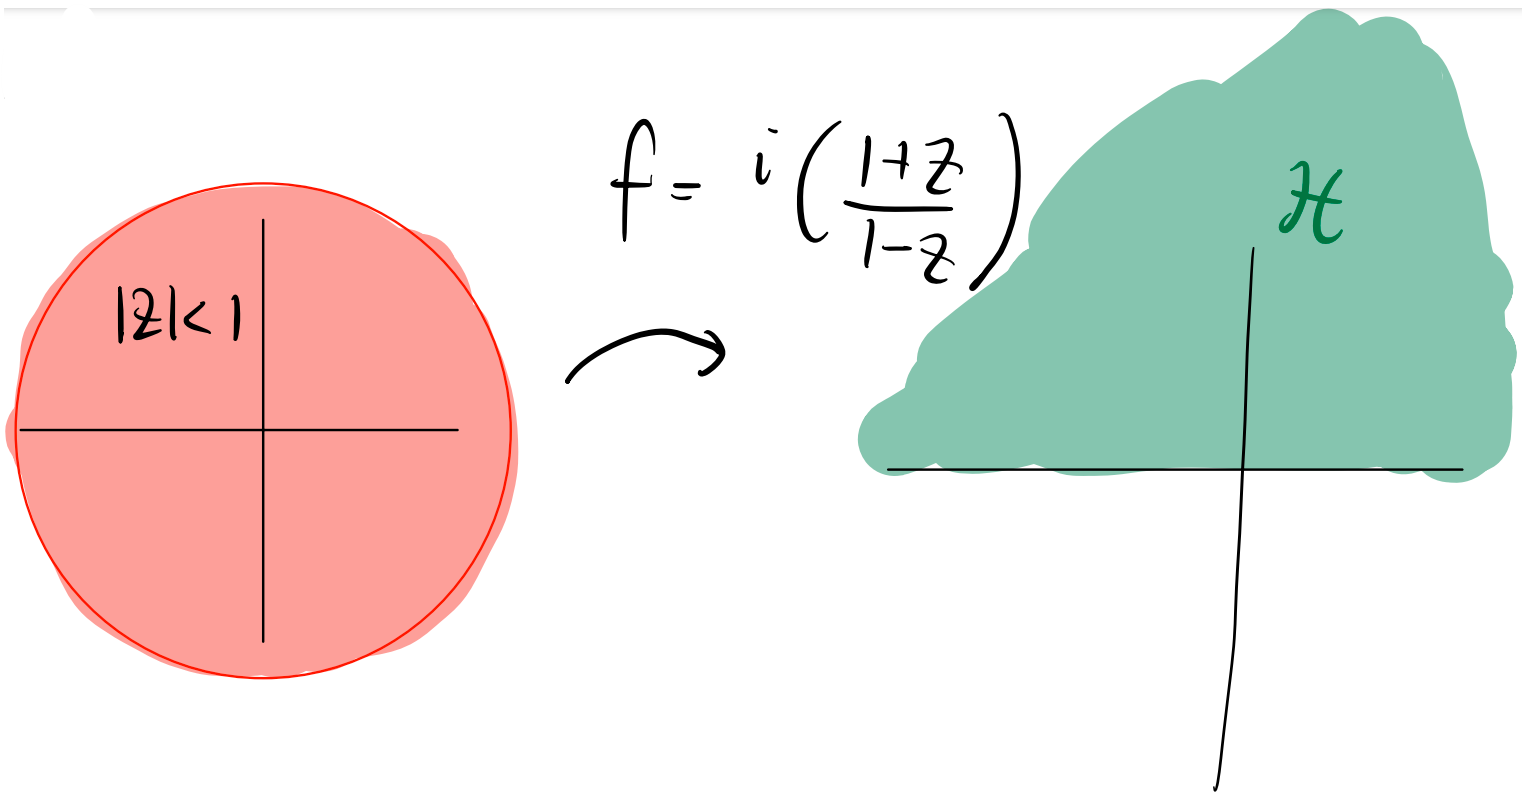
\includegraphics[width=0.5\textwidth]{LECTURE_17/graph4.png}
    \caption{Conformal Map}
\end{figure}

\begin{example}
    Mapping the upper half plane to the upper half plane plus a fraction of the lower half plane.\\
    \begin{align*}
         & h(z) = z^p \quad 0 < p < 2    \\
         & \text{Defined on } \mathbb{H}
    \end{align*}

\end{example}

\begin{figure}[H]
    \centering
    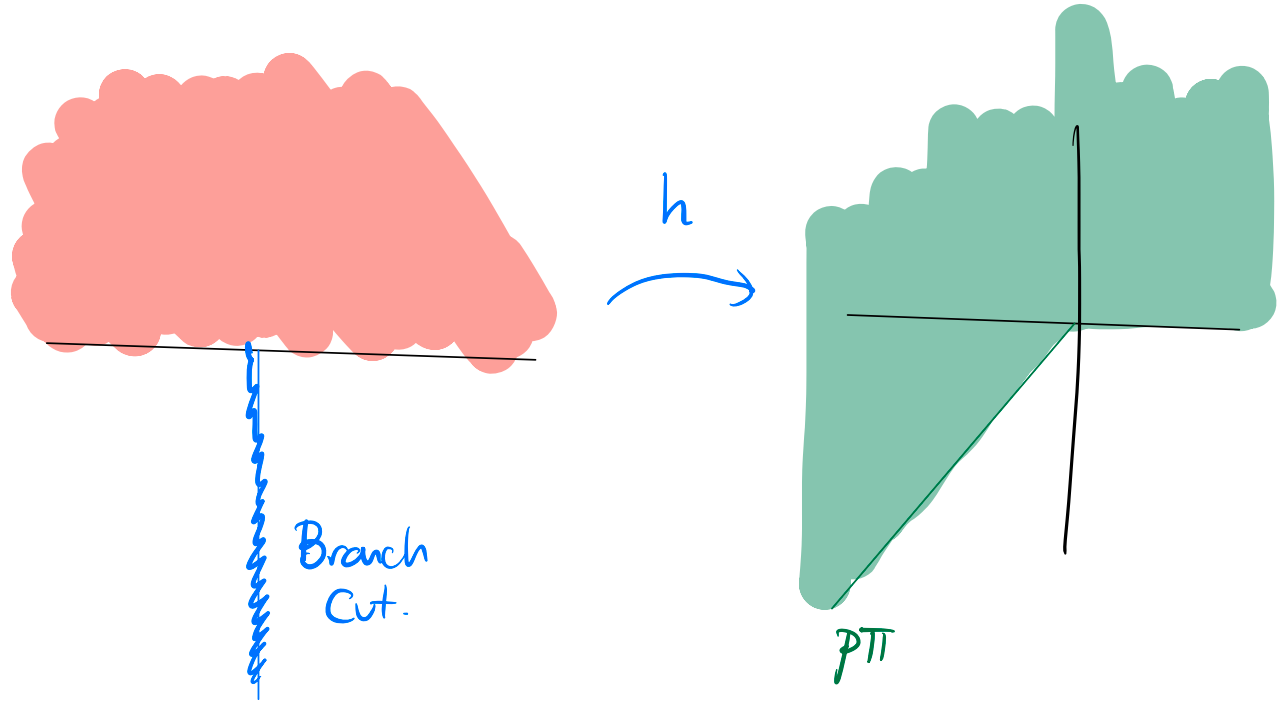
\includegraphics[width=0.5\textwidth]{LECTURE_17/graph5.png}
    \caption{Conformal Map}
\end{figure}

\section{Schwarz-Christoffel Symbols}

\begin{definition}
    This is a technique for constructing conformal maps from the upper half-plan to a polygon.
    \begin{align*}
        \mathbb{H} = \{z \in \mathbb{C} : \Im (z) > 0\} \to \text{Polygon}
    \end{align*}
\end{definition}

\begin{proposition}
    [Conformal Map from Real Numbers to Edges]
    Consider the function $f(z) = A(z - x_0)^\beta + B$ where $x_0, \beta$ are constants in $\mathbb{R}$, $0 < \beta < 2$ and $A, B$ are constants in $\mathbb{C}$. Argument chosen to lie in $(-\frac{\pi}{2}, \frac{3\pi}{2})$. \\

    Our objective is to show that $f$ maps real numbers to edges with a specific angle.
    \begin{figure}[H]
        \centering
        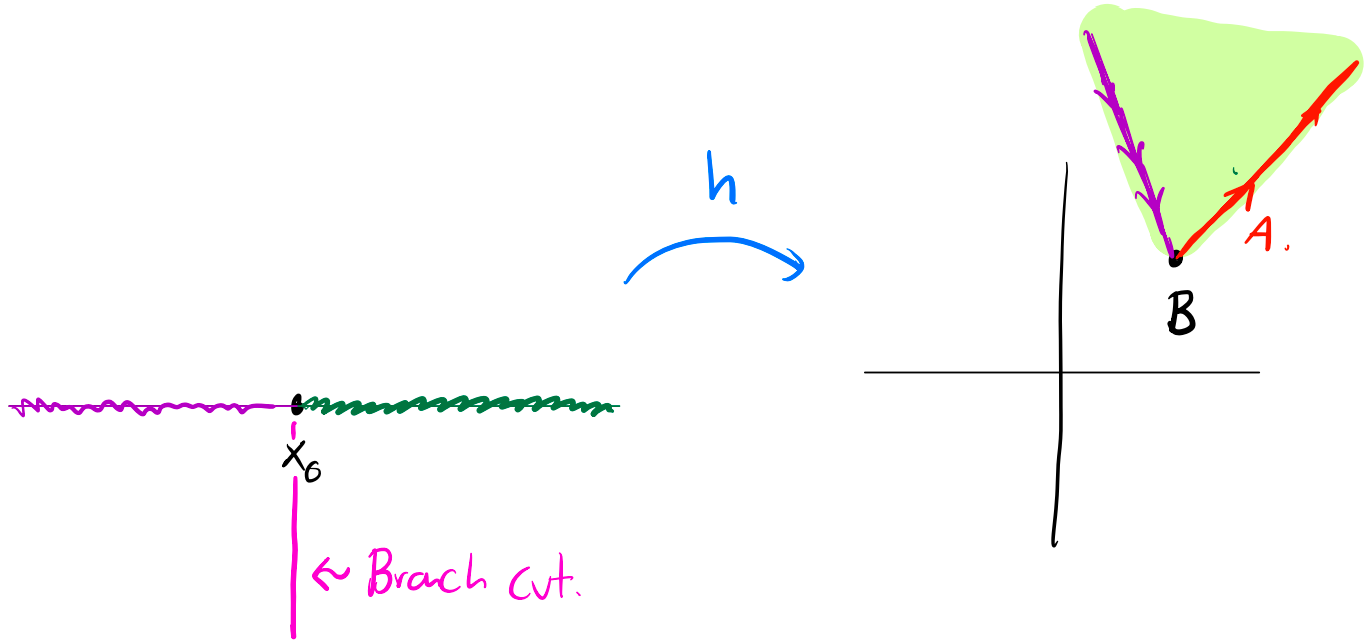
\includegraphics[width=0.5\textwidth]{LECTURE_17/graph6.png}
        \caption{Conformal Map $f$}
    \end{figure}
    We can do this by find the difference in the tangents just before and after the point $B$.\\
    Let's restrict $z$ to be real, so $z = x \in \mathbb{R}$.\\
    You can think of $f(x)$ now as a function that starts at $B$ and moves in the direction of $A$. This is true when $x > x_0$ and $\beta = 1$.\\
    \begin{figure}[H]
        \centering
        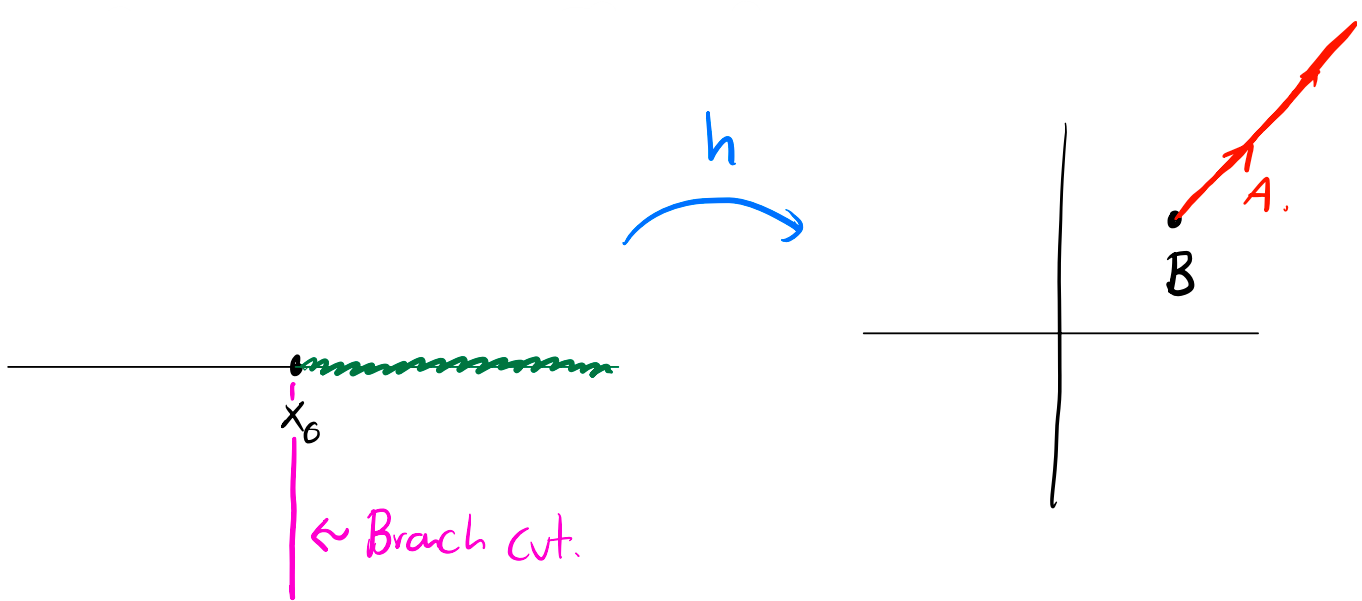
\includegraphics[width=0.5\textwidth]{LECTURE_17/graph7.png}
        \caption{Conformal Map $f$}
    \end{figure}
    Now let's write $f(x)$ in a more explicit form:
    \begin{align*}
        f(x) & = A(x - x_0)^\beta + B                                      \\
             & = Ae^{\beta \log(x - x_0)} + B                              \\
             & = Ae^{\beta \log|x - x_0| + i\beta \text{Arg}(x - x_0)} + B \\
             & = A|x - x_0|^\beta e^{i\beta \text{Arg}(x - x_0)} + B
    \end{align*}
    We can see now that $\beta$ will cause some rotation when it's not an integer.\\
    We can think of $\text{Arg}(f(z_0))$ as the angle pointing from the origin to $f(z_0)$.\\
    We can think of $\text{Arg}(f'(z_0))$ as the angle pointing from $f(z_0)$ to $f(z_0^+)$, essentially the direction of the tangent vector.\\
    With this in mind, we can find $f'(x_0^+) = B$, which the direction of the tangent vector at right after $B$.
    \begin{align*}
        f'(x)                 & = A\beta(x - x_0)^{\beta - 1}                                              \\
                              & = A\beta e^{(\beta - 1)\log|x - x_0| + i(\beta - 1)\text{Arg}(x - x_0)}    \\
                              & = A\beta |x - x_0|^{\beta - 1} e^{i(\beta - 1)\text{Arg}(x - x_0)}         \\
        f'(x_0^+)             & = A\beta |x_0^+ - x_0|^{\beta - 1} e^{i(\beta - 1)\text{Arg}(x_0^+ - x_0)} \\
        \text{Arg}(f'(x_0^+)) & = \text{Arg}(A) + (\beta - 1)\text{Arg}(x_0^+ - x_0)                       \\
                              & = \text{Arg}(A)
    \end{align*}
    The $(\beta - 1)\text{Arg}(x_0^+ - x_0) = 0$ because $x_0^+ - x_0$ is real and thus has an argument of $0$.\\
    Now we can find the tangent vector at $x_0^-$.\\
    \begin{align*}
        f'(x_0^-)             & = A\beta |x_0^- - x_0|^{\beta - 1} e^{i(\beta - 1)\text{Arg}(x_0^- - x_0)} \\
        \text{Arg}(f'(x_0^-)) & = \text{Arg}(A) + (\beta - 1)\text{Arg}(x_0^- - x_0)                       \\
                              & = \text{Arg}(A) + (\beta - 1)\pi
    \end{align*}
    Since $x_0^- - x_0$ is real and negative, it has an argument of $\pi$.\\
    Now we can find the difference in the angles of the tangent vectors at $x_0^-$ and $x_0^+$.
    \begin{align*}
        \text{Arg}(f'(x_0^+)) - \text{Arg}(f'(x_0^-)) & = \text{Arg}(A) - \text{Arg}(A) - (\beta - 1)\pi \\
                                                      & = (\beta - 1)\pi
    \end{align*}
    This means we can now map the real numbers to edges with a specific angle. We can also now see why $\beta < 2$ is required, it's because the difference between the tangents of the edges must be between $(-\pi, \pi)$.
\end{proposition}

\begin{proposition}
    [A Generalization of the Previous Proposition]
    Consider the analytic function on $\mathbb{H}$ satisfying:
    \begin{align*}
        f'(z)      & = A(z - x_1)^{\alpha_1}(z - x_2)^{\alpha_2}\ldots(z - x_n)^{\alpha_n}                                               \\
                   & \text{where } x_1 < x_2 < \ldots < x_n \in \mathbb{R} \text{ and } \alpha_1, \alpha_2, \ldots, \alpha_n \in (-1, 1) \\
        \text{Arg} & \in (-\frac{\pi}{2}, \frac{3\pi}{2})
    \end{align*}
    You can think of $\alpha_i$ as $\beta - 1$ in the previous proposition.\\
\end{proposition}

\begin{example}
    Suppose $x \in \mathbb{R}$ and $x_{j-1} < x_{j} < x_{j+1} < \ldots < x_n$. Then:
    \begin{align*}
        text{Arg}f'(x_{j}) = \text{Arg}A + \pi \alpha_{j + 1} + \ldots + \pi \alpha_n    \\
        \text{Arg}f'(x_{j+1}) = \text{Arg}A + \pi \alpha_{j + 2} + \ldots + \pi \alpha_n \\
        \therefore \text{Arg}f'(x_{j+1}) - \text{Arg}f'(x_{j}) = \pi(\alpha_{j+1})
    \end{align*}
    \begin{figure}[H]
        \centering
        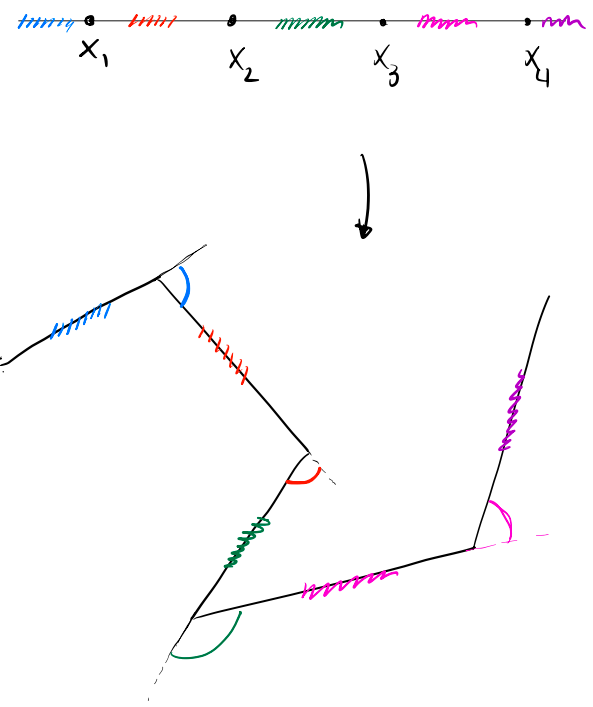
\includegraphics[width=0.5\textwidth]{LECTURE_17/graph8.png}
        \caption{Conformal Map $f$}
    \end{figure}
\end{example}

\begin{proposition}
    [Generalizing to Polygons]
    Let $P$ be a polygon with $N +1$ sides, and vertices $w_0, w_1, \ldots, w_N$. Arranged in a counter-clockwise fashion.\\
    \begin{figure}[H]
        \centering
        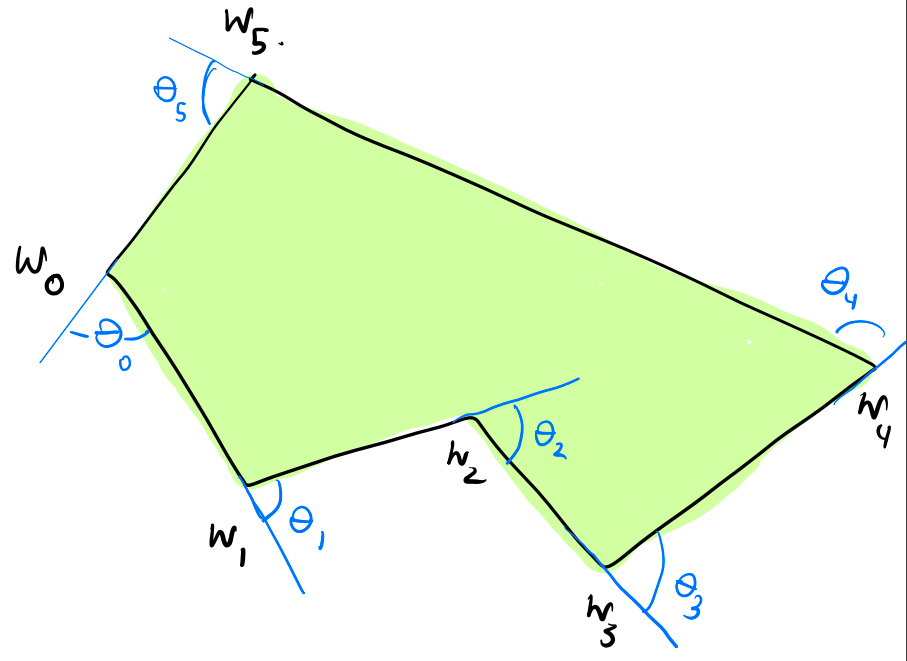
\includegraphics[width=0.5\textwidth]{LECTURE_17/graph9.png}
        \caption{Polygon $P$}
    \end{figure}

    Let $\theta_0, \theta_1, \ldots, \theta_N$ be the exterior angles of the polygon.\\
    Then we can say $\theta_0, \theta_1, \ldots, \theta_N \in (-\pi, \pi)$ and because $P$ is closed: $\theta_0 + \theta_1 + \ldots + \theta_N = 2\pi$.\\
    We know that $\alpha_j \in (-1, 1)$ so let's define $\alpha_j = -\frac{\theta_j}{\pi}$. Then:
    \begin{align*}
        \sum_{j = 0}^{N} \alpha_j = -2
    \end{align*}
\end{proposition}

\begin{theorem}
    There exists $A \in \mathbb{C}$ and real numbers $x_1 < x_2 < \ldots < x_N$ such that the Analytic function $f(z)$ on $\mathbb{H} = \{z \in \mathbb{C} : \Im (z) > 0\}$ is defined by:
    \begin{align*}
        f'(z) = A(z - x_1)^{\alpha_1}(z - x_2)^{\alpha_2}\ldots(z - x_N)^{\alpha_N}
    \end{align*}
    Which gives a 1 to 1 analytic map from $\mathbb{H}$ to the polygon $P$.
    \begin{itemize}
        \item For $j = 1, 2, \ldots, N \quad f(z_j) = w_j$. Essentially, the points $z_j | \Im (z_j) > 0$ are mapped to the inside of the polygon.
        \item $f(x) \quad x \in \mathbb{R}$ maps to the edges of the polygon.
        \item $\lim_{x \to \pm \infty} f(x) = w_0 \quad x \in \mathbb{R}$. Essentially, the points positive and negative real infinity are mapped to the left and right of the first vertex $w_0$ of the polygon.
    \end{itemize}
\end{theorem}

\begin{example}
    Find the Shwarz-Christoffel transformation taking $\mathbb{H}$ to the triangle with vertices $-a, a, i\sqrt{3}a$.
    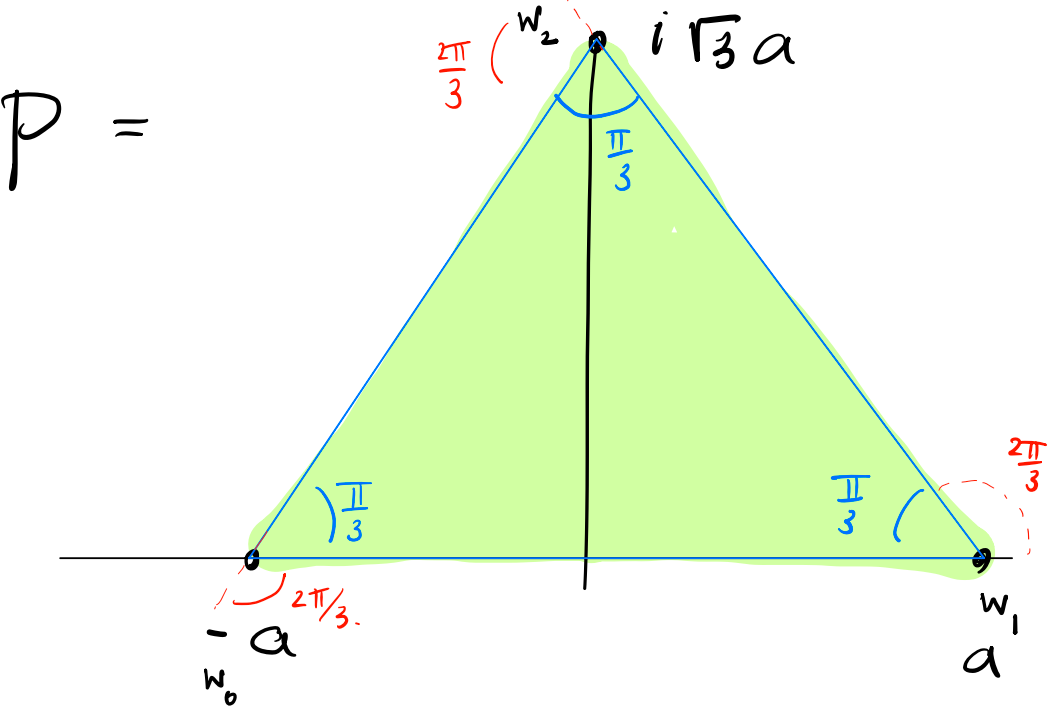
\includegraphics[width=0.5\textwidth]{LECTURE_17/graph10.png}
    The triangle has 3 sides, so $N = 2$. We choose the points $z_1 = 0, z_2 = 1$ and $z = \pm \infty$ to be mapped to the vertices of the triangle.\\
    \begin{figure}[H]
        \centering
        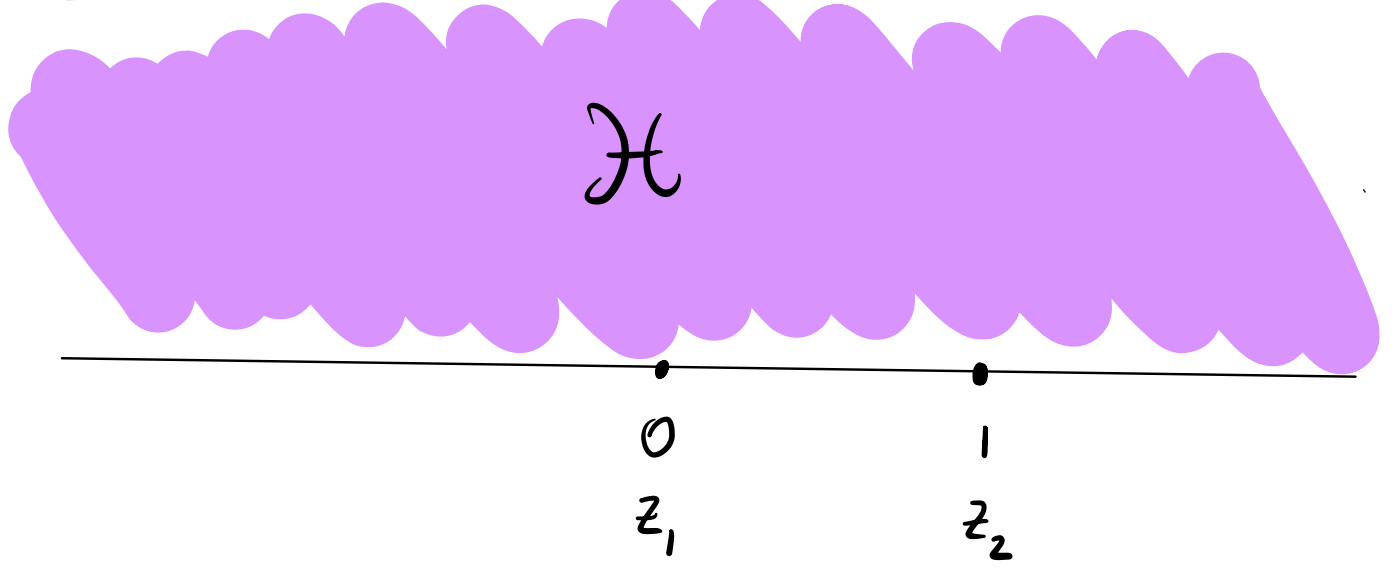
\includegraphics[width=0.5\textwidth]{LECTURE_17/graph11.png}
        \caption{Upper Half Plane with points $z_1, z_2$}
    \end{figure}
    We know that:
    \begin{align*}
        f'(z) & = A(z - x_1)^{\alpha_1}(z - x_2)^{\alpha_2} \\
        f'(z) & = A(z - 0)^{\alpha_1}(z - 1)^{\alpha_2}
    \end{align*}
    Now we can find $\alpha_1, \alpha_2$.
    \begin{align*}
        \alpha_1 = -\frac{\theta_1}{\pi} = -\frac{2\pi}{3\pi} = -\frac{2}{3} \\
        \alpha_2 = -\frac{\theta_2}{\pi} = -\frac{2\pi}{3\pi} = -\frac{2}{3}
    \end{align*}
    Now we can find $A$. Remember that any segment of the real line, as long as you don't cross the pre-image of a vertex, will have the same derivative argument as its corresponding image. So if we take the line segment $z = x \in \mathbb{R} | x < 0$ we know:
    \begin{align*}
        \text{Arg} (z)' = 0 & = \text{Arg} (f'(z))                                                        \\
                            & = \text{Arg}(A(z - x_1)^{\alpha_1}(z - x_2)^{\alpha_2})                     \\
                            & = \text{Arg}(A) + \alpha_1\text{Arg}(z - x_1) + \alpha_2\text{Arg}(z - x_2)
    \end{align*}
    Because $(z - x_1)$ and $(z - x_2)$ are real and negative, their arguments are $\pi$. So:
    \begin{align*}
        0             & = \text{Arg}(A) + \frac{2}{3}\pi + \frac{2}{3}\pi \\
        \text{Arg}(A) & = \frac{4}{3}\pi
    \end{align*}

    We can integrate to find $f(z)$.
    \begin{align*}
        f(z)      & = A\int_{1}^{z} t^{-\frac{2}{3}}(t - 1)^{-\frac{2}{3}}dt + B                       \\
        f(1)      & = A\int_{1}^{1} t^{-\frac{2}{3}}(t - 1)^{-\frac{2}{3}}dt + B                       \\
                  & = B = i\sqrt3 a                                                                    \\
        f(\infty) & = A\int_{1}^{\infty} t^{-\frac{2}{3}}(t - 1)^{-\frac{2}{3}}dt + i\sqrt3 a = -a     \\
        A         & = -a\frac{1 + i\sqrt3}{\int_{1}^{\infty} t^{-\frac{2}{3}}(t - 1)^{-\frac{2}{3}}dt}
    \end{align*}
\end{example}

\chapter{Homework 8}



\chapter{Lecture 18: Schwarz-Christoffel Mappings}

\begin{example}
    Find the Schwarz-Christoffel mapping from $\mathbb{H} = \{z \in \mathbb{C} : \Im(z) > 0\}$ to
    $$w_1 = 0 \qquad w_0 = \sigma_0 + i\tau_0\qquad \sigma_0 < 0, \tau_0 > 0$$
    \begin{figure}[H]
        \centering
        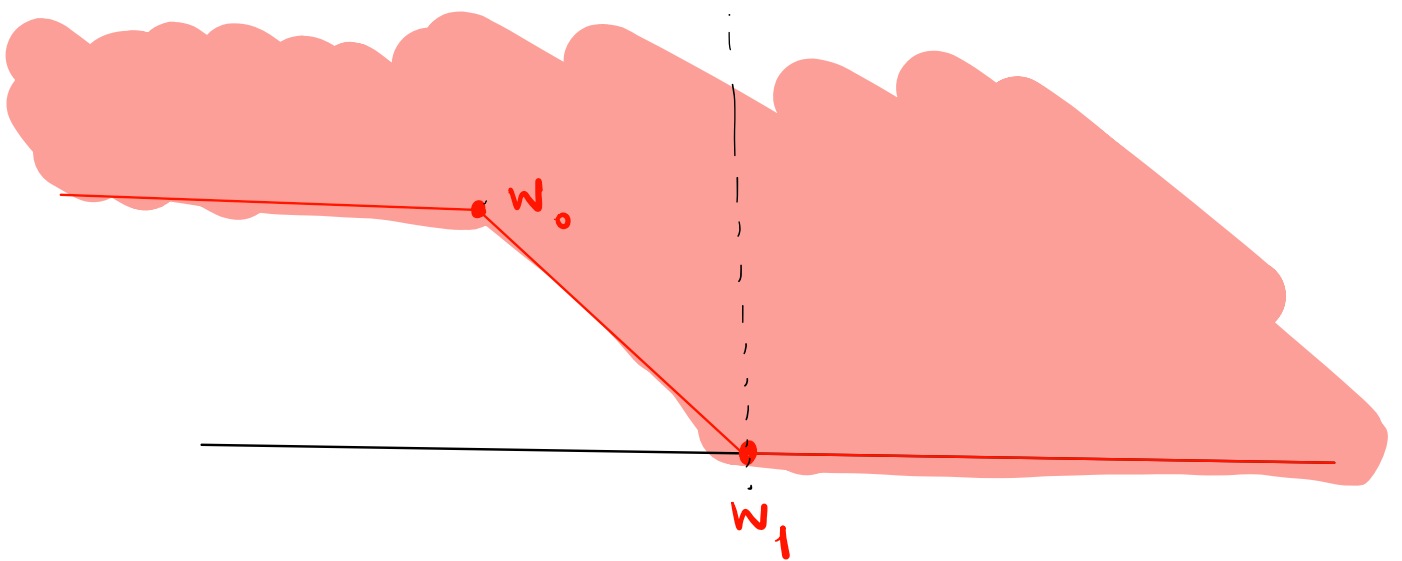
\includegraphics[width=0.5\textwidth]{LECTURE_18/graph.png}
        \caption{Graph}
    \end{figure}
    \begin{align}
        \theta_0 = \arctan(\frac{\tau_0}{\sigma_0}) \in (-\pi, 0), \quad \theta_1 = -\theta_0
    \end{align}
    We choose the points $x_0 = -1, x_1 = 1$ as the pre-image vertices. Now we write:
    \begin{align}
        f'(z) & = A (z + 1)^{-\frac{\theta_0}\pi} (z - 1)^{\frac{\theta_0}\pi}
    \end{align}
    This gives us our general form of $f'(z)$, which can't be integrated easily. So let's take a specific angle  where $\sigma_0 = 0 \rightarrow \theta_0 = -\frac{\pi}{2}$.
    \begin{figure}[H]
        \centering
        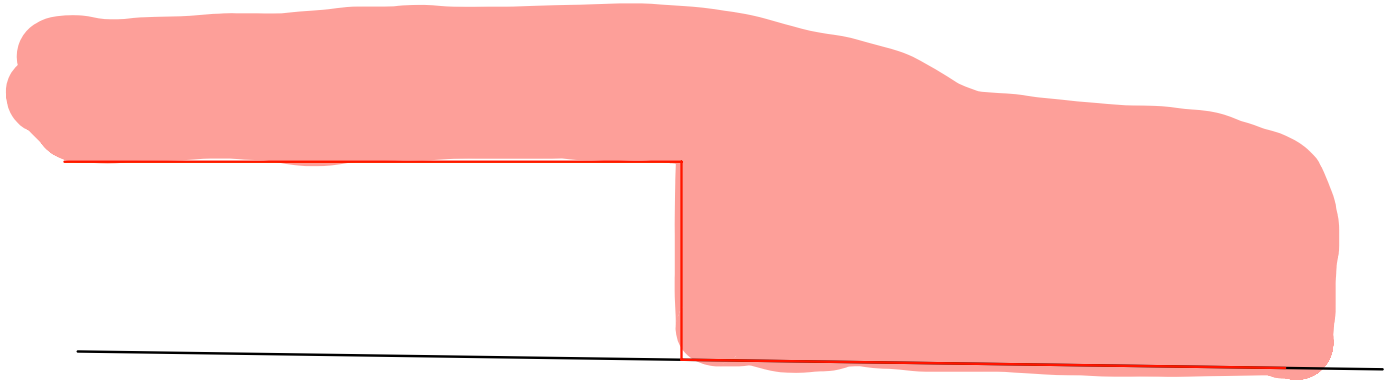
\includegraphics[width=0.5\textwidth]{LECTURE_18/graph1.png}
        \caption{Graph}
    \end{figure}
    \begin{align}
        f'(z) & = A \left(\frac{z + 1}{z - 1}\right)^{\frac{1}{2}}                                                      \\
        f'(z) & = A\left(\frac{z + 1}{z - 1}\frac{z + 1}{z + 1}\right)^{\frac{1}{2}}                                    \\
        f'(z) & = A\frac{z + 1}{(z^2 - 1)^{\frac{1}{2}}}                                                                \\
        f(z)  & = A\int \frac{z + 1}{(z^2 - 1)^{\frac{1}{2}}}dz + B                                                     \\
        f(z)  & = A\left(\int \frac{z}{(z^2 - 1)^{\frac{1}{2}}}dz + \int \frac{1}{(z^2 - 1)^{\frac{1}{2}}}dz\right) + B \\
        f(z)  & = A\left((z^2 -1)^\frac{1}2+ \text{Log}(z+ (z^2 -1)^\frac{1}2)\right) + B                               \\
    \end{align}
    Now we can find use the pre-image vertices to find $A$ and $B$. First we map $x_0 = -1$ to $w_0 = i\tau_0$:
    \begin{align}
        f(-1) & = w_0 = i\tau_0 = A\left((1 -1)^\frac{1}2+ \text{Log}(-1+ (1 -1)^\frac{1}2)\right) + B \\
              & = A(\text{Log}(-1)) + B                                                                \\
              & = A(i\pi) + B
    \end{align}
    \begin{align*}
        f(1) & = w_1 = 0 = A\left((1 -1)^\frac{1}2+ \text{Log}(1+ (1 -1)^\frac{1}2)\right) + B \\
             & = A(\text{Log}(1)) + B                                                          \\
             & = B
    \end{align*}
    This gives us $B = 0$ and $A = \frac{\tau_0}{\pi}$. So our final mapping is:
\end{example}

\begin{example}
    Find the Schwarz-Christoffel mapping from $\mathbb{H} = \{z \in \mathbb{C} : \Im(z) > 0\}$ to
    \begin{figure}[H]
        \centering
        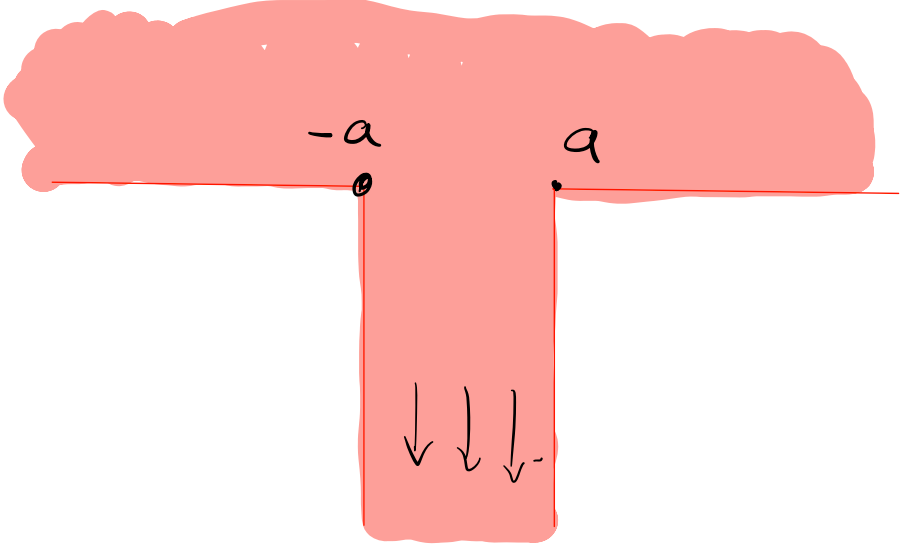
\includegraphics[width=0.5\textwidth]{LECTURE_18/graph2.png}
        \caption{Graph}
    \end{figure}
    \begin{align}
        a > 0, a \in \mathbb{R}
    \end{align}
    \textbf{Idea:} Let's approximate the valley with a triangle extending infinitely downwards
    \begin{figure}[H]
        \centering
        \includegraphics[width=0.5\textwidth]{LECTURE_18/graph3.png}
        \caption{Graph}
    \end{figure}
    We take the limit as $b \rightarrow \infty$. Then we can approximate the angles as:
    \begin{align}
        \theta_0 & = \arctan (\frac{-b}{a}) \approx \frac{-\pi}{2}                  \\
        \theta_2 & = - \arctan(\frac{b}{a}) \approx \frac{-\pi}{2}                  \\
        \theta_1 & = 0 \quad \text{triangles can only have angles that sum to } \pi
    \end{align}
    We choose the points $x_0 = -1, x_1 = 1$ as the pre-image vertices. Now we write:
    \begin{align}
        f'(z) & = A (z + 1)^{-\frac{-\theta_0}\pi}z^{\frac{-\theta_1}\pi} (z - 1)^{\frac{-\theta_2}\pi} \\
        f'(z) & = A (z + 1)^{\frac{1}{2}}z^{-1} (z - 1)^{\frac{1}{2}}                                   \\
    \end{align}
    Thus:
    \begin{align}
        f'(z) & = A\left(\frac{z^2 - 1}{z^2}\right)^{\frac{1}{2}}          \\
              & = A \sqrt{1 - \frac{1}{z^2}}                               \\
        f(z)  & = A\int \sqrt{1 - \frac{1}{z^2}}dz + B
              & = A \left(\sqrt{z^2 - 1} + \arcsin(\frac{1}{z})\right) + B
    \end{align}
    Don't worry about how the integration was done, if you're asked to do it on the exam, you're fucked. Now we can find use the pre-image vertices to find $A$ and $B$. First we map $x_0 = -1$ to $w_0 = -a$:
    \begin{align}
        f(-1) & = w_0 = -a = A \left(\sqrt{1 - 1} + \arcsin(-1)\right) + B \\
        -a    & = A \left(\arcsin(-1)\right) + B                           \\
        -a    & = A \left(-\frac{\pi}{2}\right) + B
    \end{align}
    Now we map $x_1 = 1$ to $w_1 = a$:
    \begin{align}
        f(1) & = w_1 = a = A \left(\sqrt{1 - 1} + \arcsin(1)\right) + B \\
        a    & = A \left(\arcsin(1)\right) + B                          \\
        a    & = A \left(\frac{\pi}{2}\right) + B
    \end{align}
    This gives us $B = 0$ and $A = \frac{2a}{\pi}$. So our final mapping is:
    \begin{align}
        f(z) = \frac{2a}{\pi} \left(\sqrt{z^2 - 1} + \arcsin(\frac{1}{z})\right)
    \end{align}
\end{example}

\begin{example}
    Find the Schwarz-Christoffel mapping from $\mathbb{H}/\{it \in \mathbb{C} : 0 \leq t \leq a\}$ to $\mathbb{H} = \{z \in \mathbb{C} : \Im(z) > 0\}$
    \begin{figure}[H]
        \centering
        \includegraphics[width=0.5\textwidth]{LECTURE_18/graph4.png}
        \caption{Image Mapping}
    \end{figure}
    We can observe the image vertices to be $w_0 = -\epsilon, w_1 = ia, w_2 = \epsilon$ where $\epsilon \to 0$.
    First, let's view this as the limit of the following domain:
    \begin{figure}[H]
        \centering
        \includegraphics[width=0.5\textwidth]{LECTURE_18/graph5.png}
        \caption{Domain as the limit of a triangle}
    \end{figure}
    Then we can say that the angles are:
    \begin{align}
        \theta_0 & = \frac{\pi}{2} \\
        \theta_1 & = -\pi          \\
        \theta_2 & = \frac{\pi}{2}
    \end{align}
    We choose the points $x_0 = -1, x_1 = 0, x_2 = 1$ as the pre-image vertices. Now we write:
    \begin{align}
        f'(z) & = A (z + 1)^{\frac{-1}{2}}z(z - 1)^{\frac{-1}{2}} \\
              & = A \frac{z}{\sqrt{z^2 - 1}}                      \\
        f(z)  & = A \int \frac{z}{\sqrt{z^2 - 1}}dz + B           \\
              & = A(\sqrt{z^2 - 1}) + B
    \end{align}
    Now we can find use the pre-image vertices to find $A$ and $B$. First we map $x_0 = -1$ to $w_0 = 0$:
    \begin{align}
        f(-1) = w_0 = 0 & = A(\sqrt{1 - 1}) + B \\
        0               & = B                   \\
        f(0) = w_1 = ia & = A(\sqrt{0 - 1})     \\
        A = a                                   \\
    \end{align}
    This gives us $B = 0$ and $A = a$. So our final mapping is:
    \begin{align}
        f(z) = a\sqrt{z^2 - 1}
    \end{align}
\end{example}

\chapter{Fluid Flows \& Harmonic Functions}

\begin{proposition}
    Suppose $D \subseteq \mathbb{C} (= \mathbb{R}^2)$ and the following kind of flow fluid flowing through $D$.
    \begin{figure}[H]
        \centering
        \includegraphics[width=0.5\textwidth]{LECTURE_19/graph.png}
        \caption{Fluid Flow through $D$}
    \end{figure}
    \textbf{We assume:}
    \begin{enumerate}
        \item[(i)] The flow is in a \textbf{steady state} (velocity doesn't change with time).
        \item[] The direction of the flow at $(x,y) \in D$ is given by a vector field $\mathbf{v}(x,y) = (u(x,y), v(x,y))$.
        \item[(ii)] the flow is \textbf{irrotational}, imagine a small paddle wheel at $(x,y)$, it doesn't rotate.
        \item[] \begin{figure}[H]
                  \centering
                  \begin{subfigure}{0.4\textwidth}
                      \centering
                      \includegraphics[width=\textwidth]{LECTURE_19/irrotational.png}
                      \caption{Irrotational Flow}
                  \end{subfigure}
                  \hfill
                  \begin{subfigure}{0.4\textwidth}
                      \centering
                      \includegraphics[width=\textwidth]{LECTURE_19/rotational.png}
                      \caption{Rotational Flow}
                  \end{subfigure}
              \end{figure}
        \item[] \textbf{Mathematically:} $\frac{\partial v}{\partial x} = \frac{\partial u}{\partial y}, \quad \forall (x,y) \in D$.
        \item[] You can think of $\frac{\partial v}{\partial x}$ as the change in vertical velocity as you move in the horizontal direction. Essentially, the amount of $x$ rotation (counter clockwise). Similarly, $\frac{\partial u}{\partial y}$ is the amount of $y$ rotation (clockwise). Therefore, if there is a horizontal rotation, there must be a vertical rotation to maintain irrotationality.
        \item[(iii)] The flow is \textbf{sourceless/sinkless}, no fluid is created or destroyed (incompressible).
        \item[] \textbf{Mathematically:} $\frac{\partial u}{\partial x} + \frac{\partial v}{\partial y} = 0, \quad \forall (x,y) \in D$.
        \item[] You can think of $\frac{\partial u}{\partial x}$ as the change in horizontal velocity as you move in the horizontal direction. Essentially, the amount of $x$ stretch/compression. Similarly, $\frac{\partial v}{\partial y}$ is the amount of $y$ stretch/compression. Therefore, if there is a horizontal stretch, there must be a vertical stretch to maintain the same volume.
    \end{enumerate}
\end{proposition}

\begin{remark}
    For a function $f(z)$ that is analytic in $D$, and the independent variable $z = x + iy$ where $x,y \in \mathbb{R}$, we can define $\frac{\partial}{\partial z}$ and $\frac{\partial}{\partial \overline{z}}$ as follows:
    \begin{align*}
        \frac{\partial}{\partial z} = \frac{1}2\left(\frac{\partial}{\partial x} - i\frac{\partial}{\partial y}\right), \quad \frac{\partial}{\partial \overline{z}} = \frac{1}2\left(\frac{\partial}{\partial x} + i\frac{\partial}{\partial y}\right)
    \end{align*}
\end{remark}

\begin{corollary}
    [Cauchy-Riemann Equations for Flows]
    If $\mathbf{v}(x,y) = (u(x,y), v(x,y))$ is a sourcelss irrotational flow then:
    \begin{enumerate}
        \item[(i)] $\Delta u = \frac{\partial^2 u}{\partial x^2} + \frac{\partial^2 u}{\partial y^2} = 0$.
        \item[(ii)] $\Delta v = \frac{\partial^2 v}{\partial x^2} + \frac{\partial^2 v}{\partial y^2} = 0$.
        \item[(iii)] $\overline{f} = u - iv$ is analytic in $D$ by the Cauchy-Riemann equations.
    \end{enumerate}

    \textbf{Furthermore,} there exists an analytic function $G$ on $D$ such that $G' = \overline{f}$ on $D$.
    \begin{proof}
        Why must there exist such a $G$?\\
        Because sources and irrotational flows imply $\int_\gamma \overline{f} dz = 0 \quad \forall$ closed curves $\gamma$ and vice-versa.
    \end{proof}
    Now then, by (the proof of) Morera's Theorem
    \begin{align*}
        G                 & = \phi + i \psi                                                                                                                                                                                \\
        \frac{dG}{dz}     & = \frac{1}2\left[\frac{\partial G}{\partial x} - i\frac{\partial G}{\partial y}\right]                                                                                                         \\
                          & = \frac{1}2\left[\left(\frac{\partial \phi}{\partial x} + i\frac{\partial \psi}{\partial x}\right) - i\left(\frac{\partial \phi}{\partial y} + i\frac{\partial \psi}{\partial y}\right)\right] \\
                          & \rightarrow \text{Now we can separate the real and imaginary parts}                                                                                                                            \\
                          & = \frac{1}2\left[\left(\frac{\partial \phi}{\partial x} + \frac{\partial \psi}{\partial y}\right) + i\left(\frac{\partial \psi}{\partial x} - \frac{\partial \phi}{\partial y}\right)\right]   \\
                          & \rightarrow \text{We know } \overline{f} = G' \text{ is analytic}                                                                                                                              \\
                          & \rightarrow \text{Then } G \text{ must be analytic and follow the Cauchy-Riemann equations}                                                                                                    \\
                          & \rightarrow \frac{\partial \phi}{\partial x} + \frac{\partial \psi}{\partial y} = 2\frac{\partial \phi}{\partial x}                                                                            \\
                          & \rightarrow \frac{\partial \psi}{\partial x} - \frac{\partial \phi}{\partial y} = 2\frac{\partial \psi}{\partial x}                                                                            \\
        G'= \overline{f}  & = \underbrace{\frac{\partial \phi}{\partial x}}_{u} + i\underbrace{\frac{\partial \psi}{\partial x}}_{-v}                                                                                      \\
        G' = \overline{f} & = \underbrace{\frac{\partial \psi}{\partial y}}_u - i\underbrace{\frac{\partial \phi}{\partial y}}_{v}
    \end{align*}
    So:
    \begin{align*}
        \nabla \phi & = (u,v) = \left(\frac{\partial \phi}{\partial x}, \frac{\partial \phi}{\partial y}\right)  \\
        \nabla \psi & = (-v,u) = \left(\frac{\partial \psi}{\partial x}, \frac{\partial \psi}{\partial y}\right)
    \end{align*}
    Thus:
    \begin{enumerate}
        \item[(i)] The level sets of $\{\phi = c\}$ are orthogonal to the flow
        \item[(ii)] The level sets of $\{\psi = c\}$ are flow lines.
    \end{enumerate}
    \textbf{$\phi$ is called the \underline{potential function}}
    \textbf{$\psi$ is called the \underline{stream function}.}
\end{corollary}

\begin{remark}
    \begin{itemize}
        \item[]
        \item The sets $\{\phi(x,y) = c\}$ are sets with equal potential energy at different $(x,y)$. Hence $\phi$ is called the potential function.
        \item The sets $\{\psi(x,y) = c\}$ are streamlines of the flow . Hence $\psi$ is called the stream function.
    \end{itemize}
\end{remark}

\begin{figure}[H]
    \centering
    \includegraphics[width=0.5\textwidth]{LECTURE_19/potential-and-stream.png}
    \caption{Potential and Stream Functions}
\end{figure}

\begin{example}
    Find the flow lines of a sourceless irrotational flow past a wall of height $a$ (assuming take height is $>> a$).
    \begin{figure}[H]
        \centering
        \includegraphics[width=0.5\textwidth]{LECTURE_19/graph1.png}
        \caption{Fluid Flow past a wall}
    \end{figure}
    \textbf{Solution:}
    Since the fluid can't flow through the wall, the flow lines must be orthogonal ($\nabla \phi = (u,v) = (0, v)$) to the wall on $x =0 ,\quad 0 \leq y \leq a$. We can solve this with conformal mapping. Our idea is we'll have a domain with a flow from left to right. We'll take the flow lines of that flow and map it to our domain with the wall. We'll then have the flow lines around the wall. \\
    Recall that $f(z) = a(z^2 - 1)^{1/2}$ defines a conformal map from $\mathbb{H}/\{it \in \mathbb{C} : 0 \leq t \leq a\}$ to the upper half plane, sending $f(-1) = f(1) = 0$. Let's consider the right moving flow in the pre-image $\mathbb{H}$:
    \begin{align*}
        (\tilde{u}, \tilde{v}) = (1, 0) \\
        \tilde{G} = z = x + iy
    \end{align*}
    Whose flow lines are given by $\{\Im(z) = y\}$ because there's only one component of velocity (there are no vertical flow lines), so we observe the flow at different values of $y$.\\
    The Image of these flow lines is under $f$ will be the flow lines around the wall $(a = 1)$.
    \begin{align*}
        f(x + iy) & = (z^2 - 1)^{\frac{1}2} = \sqrt{z -1}\sqrt{z + 1}                                                                                                                \\
                  & = \sqrt{(x + iy) - 1}\sqrt{(x + iy) + 1}                                                                                                                         \\
                  & = ((x -1) + y)^{1/2}((x+1) + y)^{1/2}                                                                                                                            \\
                  & = \pm|(x -1) + iy|^{1/2}e^{\frac{i}2\arg(x + iy - 1)}\times \pm|(x+1) + iy|^{1/2}e^{\frac{i}2\arg(x + iy + 1)}                                                   \\
                  & \rightarrow \arg(x + iy - 1) = \cos^{-1}\left(\frac{\Re(x + iy - 1)}{|x + iy - 1|}\right) = \cos^{-1}\left(\frac{x -1}{\sqrt{(x-1)^2 + y^2}}\right)              \\
                  & = ((x -1)^2 + y^2)^{1/4}e^{\frac{i}2\cos^{-1}(\frac{x -1}{\sqrt{(x-1)^2 + y^2}})}((x+1)^2 + y^2)^{1/4}e^{\frac{i}2\cos^{-1}(\frac{x + 1}{\sqrt{(x+1)^2 + y^2}})}
    \end{align*}
    \textbf{Note:} the root is multi-valued, because a conformal map is definite (and it doesn't make sense for a fluid to have two different directions in the same place), we have to choose a value. We choose the positive value to keep us in the upper-half plane.
    \begin{align*}
         & \text{x-component of the flow} =                                                                                                                                    \\
         & ((x- 1)^2 + y^2)^{1/4}((x+1)^2 + y^2)^{1/4}\cos(\frac{1}2\left(\cos^{-1}(\frac{x -1}{\sqrt{(x-1)^2 + y^2}}) + \cos^{-1}(\frac{x + 1}{\sqrt{(x+1)^2 + y^2})}\right)) \\
         & \text{y-component of the flow} =                                                                                                                                    \\
         & ((x- 1)^2 + y^2)^{1/4}((x+1)^2 + y^2)^{1/4}\sin(\frac{1}2\left(\cos^{-1}(\frac{x -1}{\sqrt{(x-1)^2 + y^2}}) + \cos^{-1}(\frac{x + 1}{\sqrt{(x+1)^2 + y^2})}\right))
    \end{align*}

    \begin{figure}[H]
        \centering
        \includegraphics[width=0.5\textwidth]{LECTURE_19/resultant-flow.png}
        \caption{Flow Lines around the wall}

    \end{figure}

\end{example}

\begin{example}
    Find the flow lines of a sourceless irrotational flow past an infinitely deep trench.
    \begin{figure}[H]
        \centering
        \includegraphics[width=0.5\textwidth]{LECTURE_19/trench.png}
        \caption{Fluid Flow past a trench}
    \end{figure}
    \textbf{Solution:}
    Recall that:
    \begin{align*}
        f(z) = \frac{2}\pi((z^2 -1)^{1/2} + \arcsin(\frac{1}z))
    \end{align*}
    Defines a conformal map from $\mathbb{H} \to$ the an infinitely deep trench from $-a$ to $a$.

    Consider the right moving flow
    \begin{align*}
        (\tilde{u}, \tilde{v}) = (1, 0)
    \end{align*}
    The flow lines through the trench are the image of the flow lines $\{\Im(z) = y\}$ under $f$.
    \begin{align*}
        f(x + iy) & = \sqrt{(x + iy) - 1}\sqrt{(x + iy) + 1}                                                                                                                                     \\
                  & = \frac{2}\pi[((x -1)^2 + y^2)^{1/4}e^{\frac{i}2\cos^{-1}(\frac{x -1}{\sqrt{(x-1)^2 + y^2}})}((x+1)^2 + y^2)^{1/4}e^{\frac{i}2\cos^{-1}(\frac{x + 1}{\sqrt{(x+1)^2 + y^2})}} \\
                  & + \arcsin(\frac{1}{x + iy})]
    \end{align*}

    \begin{figure}[H]
        \centering
        \includegraphics[width=0.5\textwidth]{LECTURE_19/trench-flow.png}
        \caption{Flow Lines through the trench}
    \end{figure}
\end{example}


\begin{example}
    [Fluid Flow Past a Solid Body]
    Lets Assume the flow is (locally) sourceless and irrotational.
    \begin{figure}[H]
        \centering
        \includegraphics[width=0.75\textwidth]{LECTURE_19/flow-past-body.png}
        \caption{Fluid Flow past a solid body}
    \end{figure}
    \begin{itemize}
        \item $\Gamma$ is the simple closed curve, piecewise $C^1$ boundary around body.
        \item $\Omega$ is the region inside the body.
        \item $\gamma$ is some simple, closed, piecewise $C^1$, positively oriented curve such that $\Omega \subseteq$ inside$(\gamma)$.
        \item $\overline{f} = u - iv$ is analytic outside $\Omega$
    \end{itemize}
    We call $\tau = \frac{\gamma'}{|\gamma'|}$ the tangent unit vector to $\gamma$, $C$ the circulation of the flow around $\Omega$, and $ds = |\gamma'|dt$ the arc length element of $\gamma$.
    \begin{align*}
        C & = \int_\gamma f (\gamma') \cdot \tau \, ds                                                                               \\
          & = \int_\gamma (u + iv) \cdot \frac{\gamma'}{|\gamma'|} \, |\gamma'| \, dt                                                \\
          & = \int_\gamma \Re((u + iv) \cdot (\Re(\gamma') + i\Im(\gamma'))) \, dt \quad \text{Since the dot product is always real} \\
          & = \Re(\int_\gamma (u\Re(\gamma') - v\Im(\gamma')) \, dt)                                                                 \\
          & = \Re(\int_\gamma \overline{f} \gamma' \, dt)                                                                            \\
          & =\Re\left(\int_\gamma \overline{f} (\gamma')\gamma'dt\right) \quad \text{if } z = \gamma(t)                              \\
          & = \Re\left(\int_\gamma \overline{f} dz\right)                                                                            \\
    \end{align*}
    \textbf{Note:} $C$ does not depend on $\gamma$ by Cauchy's Theorem. Since $\overline{f}$ is analytic in $\Omega$.
    Since the flow goes around $\Omega$, and hence, there's no flow come out through the surface of the body:
    \begin{align*}
        (u,v) \cdot \vec{\eta} = 0 \quad \text{ on } \partial \Omega
    \end{align*}
    Where $\vec{\eta} = (\cos\theta, \sin\theta)$ (where $\theta = \arg(\vec{\eta})$) is the outward unit normal to $\partial \Omega$. So if you have a vertical wall, $\cos \theta = 0$ and thus $u\cos\theta = 0$ for all vertical flows, which makes sense since the flow is parallel to the wall. Similar for horizontal walls.\\
    So let's take the parametrization $\Gamma(t), \quad ds = |\Gamma'(t)|dt$ of $\partial \Omega$.
    \begin{align*}
        0 & = \int_{\partial \Omega =\Gamma} f(\Gamma(t)) \cdot \vec{\eta} \quad \Gamma'(t) \, dt
          & = \int_{\partial \Omega =\Gamma} (u + iv) \cdot (\cos\theta + i\sin\theta)
    \end{align*}
    \begin{align*}
        0 & = \int_{\partial \Omega =\Gamma} f \cdot \vec{\eta} \, dt                             \\
          & = \int_{\partial \Omega =\Gamma} (u + iv) \cdot (\cos\theta + i\sin\theta)
          & = \int_{\Gamma} \Re((u + iv) \cdot (-\tau_y + i\tau_x)) \, ds                         \\
          & = \int_{\Gamma} \Re((u + iv) \cdot (-\Im(\tau) + i\Re(\tau))) \, ds                   \\
          & = \int_{\Gamma} -u\Im(\tau) - v\Re(\tau) \, ds                                        \\
          & = \Im(\int_{\Gamma} \overline{f}(z) \, dz) = \Im(\int_{\Gamma} \overline{f}(z) \, dz)
    \end{align*}
    Assume the flow is uniform far from $\Omega$.
    \begin{figure}[H]
        \centering
        \includegraphics[width=\textwidth]{LECTURE_19/uniform.png}
        \caption{Uniform Flow}

    \end{figure}
    \begin{align*}
        \lim_{|z| \to \infty} \overline{f}(z) = a \in \mathbb{C}
    \end{align*}
    Thus, $\overline{f}$ has a removable singularity at $\infty$.
    i.e. If we set $w = \frac{1}z$ then $h(w) = \overline{f}(\frac{1}w)$ is analytic in $\{0 < |w| < \epsilon\}$ and bounded as $w \to 0$.\\
    Since $\overline{f}$ is analytic and has a removable singularity at $\infty$, it has a power series expansion at $\infty$.
    \begin{align*}
        \overline{f} = \sum_{k = 0}^{\infty}b_k(\frac{1}z)^k
    \end{align*}
    is valid for $|z|$ large.
    \begin{align*}
        \lim_{|z| \to \infty} \overline{f} & = \lim_{|z| \to \infty} \left(b_0 + \frac{b_1}z + \sum_{k = 2}^{\infty}b_k(\frac{1}z)^k\right) \\
        b_0                                & = a = \lim_{|z| \to \infty} f(z)                                                               \\
    \end{align*}
    Cauchy's Integral Formula can be used to find coefficients in a power series expansion.
    \begin{align*}
        b_k & = \frac{1}{2\pi i}\int_{|z| = R} \frac{\overline{f}(z)}{z^{k-1}} \, dz                         \\
            & = \frac{1}{2\pi i}\int_{|z| = R} \overline{f}(z) \, dz                                         \\
        b_1 & = \frac{C}{2\pi i} \quad \text{where} \quad C = \text{circulation of the flow around $\Omega$}
    \end{align*}
    This gives us the final result:
    \begin{align*}
        \overline{f}(z) = a + \frac{C}{2\pi i z} + \sum_{k = 2}^{\infty}b_k(\frac{1}z)^k
    \end{align*}

    \textbf{Our Goal: }To fix $C$, to get some $\overline{f}$ such that $\overline{f} \cdot \vec{\eta}|_\Gamma = 0$ on $\partial \Omega$.\\

\end{example}

\begin{proposition}
    [Kutta-Joukowski Theorem]
    Assume $\Omega$ has density $\rho$.\\
    \textbf{We can compute:} The total vertical force, $V$, and horizontal force $H$ on $\Omega$ due to the flow.
    \begin{align*}
        \boxed{V + iH = -\rho C a}
    \end{align*}
    If $a \in R$, then the only force is vertical, the lift force.
\end{proposition}

\begin{definition}
    [Unit Tangent \& Normal Vectors]
    Say we have some body $\Omega$ with boundary parametrized by $\Gamma(t)$. The unit tangent vector is:
    \begin{align}
        \tau = \frac{\Gamma'}{|\Gamma'|}
    \end{align}
    The unit normal vector is a clockwise $90^\circ$ rotation, which can be achieved by multiplying by $-i$, you can remember this by remembering how the vector $(1,0)$ rotates after multiplying by $i$ or $-i$.
    \begin{align}
        \eta = -i\tau = \frac{-i\Gamma'}{|\Gamma'|}
    \end{align}
    \begin{figure}[H]
        \centering
        \includegraphics[width=0.5\textwidth]{LECTURE_19/unit.jpg}
        \caption{Unit Tangent and Normal Vectors}
    \end{figure}
\end{definition}

\begin{example}
    [Flow Past a Disk]
    \begin{align*}
        \Omega = \{|z| < 1\}                        \\
        \lim_{|z| \to \infty} \overline{f} = (1, 0) \\
    \end{align*}
    \begin{figure}[H]
        \centering
        \includegraphics[width=\textwidth]{LECTURE_19/disk.png}
        \caption{Fluid Flow past a disk}
    \end{figure}
    \textbf{Therefore we want}
    \begin{align*}
        \overline{f} & = a + \frac{C}{2\pi i z} + \sum_{k = 2}^{\infty}b_k(\frac{1}z)^k \\
        \overline{f} & = 1 + \frac{C}{2\pi i z} + \sum_{k = 2}^{\infty}b_k(\frac{1}z)^k
    \end{align*}
    Such that on $\partial \Gamma$, $\Gamma(t) = e^{it}, \quad 0 \leq t \leq 2\pi$ which will parametrize a unit circle. First we find $\vec{\eta}$:
    \begin{align}
        \vec{\eta} & = -i\tau                       \\
                   & = -i\frac{\Gamma'}{|\Gamma'|}  \\
                   & = -i\frac{i e^{it}}{|ie^{it}|} \\
                   & = e^{it}
    \end{align}
    Now we want $\overline{f} \cdot \vec{\eta} = 0$ on $\partial \Omega$.
    \begin{align*}
        0 & = f(\Gamma) \cdot \eta                                            \\
          & = (u,v)\cdot(\cos\theta,\sin\theta)                               \\
          & = u\cos\theta + v\sin\theta                                       \\
          & = \Re((u - iv) (\cos\theta + i\sin\theta))                        \\
          & \rightarrow e^{i\theta} = \cos\theta + i\sin\theta                \\
          & = \Re((u - iv)e^{i\theta}) = \Re(\overline{f}(\Gamma)e^{i\theta})
    \end{align*}
    This way we can use what we know about $\overline{f}$
    \begin{align*}
        \Re\left[(1 + \frac{C}{2\pi i}e^{-i\theta} + \sum_{k = 2}^{\infty}b_k e^{-ik\theta})e^{i\theta}\right]       & = 0 \\
        \Re\left[\frac{C}{2\pi i} + e^{i\theta} + b_2e^{-i\theta} + \sum_{k = 3}^{\infty}b_k e^{i(1-k)\theta}\right] & = 0
    \end{align*}
    In order to make $\Re(\frac{C}{2\pi i}) = 0$, we must have $C$ be real so the whole term is imaginary.\\
    We can have $b_2e^{-i\theta}$ cancel out $e^{i\theta}$:
    \begin{align}
        \Re(e^{i\theta} + b_2e^{-i\theta}) & = \Re(\cos\theta + i\sin\theta + b_2(\cos(-\theta) + i\sin(-\theta))) \\
                                           & = \cos\theta + b_2\cos(-\theta)                                       \\
                                           & = \cos\theta + b_2\cos\theta = 0 \quad \text{if } b_2 = -1
    \end{align}
    Lastly, we can set $b_k = 0$ for $k \geq 3$ to make the sum term zero.\\
    In summary:
    \begin{align*}
        C\in \mathbb{R}, \quad b_2 = -1, \quad b_k = 0 \quad \forall k \geq 3
    \end{align*}
    Therefore:
    \begin{align*}
        \overline{f} = 1 - \frac{C}{2\pi i z} - \frac{1}{z^2}
    \end{align*}
    We can extend this analysis to other domains using conformal maps (e.g. conformal map $\phi$)\\ A common example is the Joukowski airfoil:
    \begin{align*}
        \Omega  & = {|z - z_0| < R}     \\
        \phi(z) & = (z + \frac{R^2}{z})
    \end{align*}

    \begin{figure}[H]
        \centering
        \includegraphics[width=0.5\textwidth]{LECTURE_19/airfoil.png}
        \caption{Conformal Map of a Disk}
    \end{figure}
    \begin{itemize}
        \item The circulation is determined by $z_0, \quad R$.
        \item The lift force is determined by $\Im(z_0)$.
    \end{itemize}
\end{example}


\chapter{Homework 9}

\begin{example}
    [Fisher, Section 3.5, Problem 2]
    Find a conformal map from
    $D = \{ z \in \mathbb{C} : |\text{Arg}(z)| < \alpha \} \quad \text{for } 0 < \alpha \leq \pi,$
    to the upper half-plane
    $\mathcal{H} = \{ w \in \mathbb{C} : \text{Im}(w) > 0 \}$.

    \hrule
    \vspace{0.5cm}
    % A conformal map $w = f(z)$ preserves angles and maps the wedge-shaped region $D$ to the upper half-plane $\mathcal{H}$. The basic idea is:
    % \begin{itemize}
    %     \item Use a power map $z^p$ to "open up" or "flatten" the wedge.
    %     \item Possibly include a rotation to align the mapped region correctly with $\mathcal{H}$.
    %     \item Ensure the resulting map transforms the boundaries of $D$ to the real axis of $\mathcal{H}$, with the interior of $D$ mapped to the upper half-plane.
    % \end{itemize}

    The wedge $D$ is symmetric about the real axis, with boundaries given by:
    \begin{align*}
        \operatorname{Arg}(z) & = \pm \alpha.
    \end{align*}

    We will use the function:
    \[
        f(z) = \left( z^{\frac{\pi}{2\alpha}} \right) e^{i\frac{\pi}{2}}.
    \]

    Express $z$ in polar form:
    \begin{align*}
        z    & = r e^{i\theta}, \quad \text{so}                                                                            \\
        f(z) & = \left( r^{\frac{\pi}{2\alpha}} e^{i \left( \frac{\pi}{2\alpha} \theta \right)} \right) e^{i\frac{\pi}{2}} \\
             & = r^{\frac{\pi}{2\alpha}} e^{i \left( \frac{\pi}{2\alpha} \theta + \frac{\pi}{2} \right)}.
    \end{align*}

    When $\theta = -\alpha$ (the boundaries of $D$):
    \begin{align*}
        \operatorname{Arg}(f(z)) & = \frac{\pi}{2\alpha} (-\alpha) + \frac{\pi}{2} = -\frac{\pi}{2} + \frac{\pi}{2} = 0.
    \end{align*}

    When $\theta = \alpha$:
    \begin{align*}
        \operatorname{Arg}(f(z)) & = \frac{\pi}{2\alpha} (\alpha) + \frac{\pi}{2} = \frac{\pi}{2} + \frac{\pi}{2} = \pi.
    \end{align*}

    This maps the boundaries of $D$ to the real axis $(\operatorname{Im}(w) = 0)$.

    For $|\operatorname{Arg}(z)| < \alpha$ (the interior of $D$), we have:
    \begin{align*}
        -\alpha < \theta < \alpha \implies -\frac{\pi}{2} + \frac{\pi}{2} < \operatorname{Arg}(f(z)) < \frac{\pi}{2} + \frac{\pi}{2} \implies 0 < \operatorname{Arg}(f(z)) < \pi.
    \end{align*}
    This places the image of the interior of $D$ in the upper half-plane $(\operatorname{Im}(w) > 0)$.

    Thus, the function $f(z) = \left( z^{\frac{\pi}{2\alpha}} \right) e^{i\frac{\pi}{2}}$ is a conformal map from $D$ to $\mathcal{H}$.

    This map transforms the wedge $D$ with angle $2\alpha$ into the upper half-plane, preserving the conformal property.

\end{example}

\begin{example}
    [Fisher, Section 3.5, Problem 3]

    Find a conformal map from $D = \{ x + iy \in \mathbb{C} : |y - 1| < 2 \}$ to the upper half-plane $\mathcal{H} = \{ w \in \mathbb{C} : \operatorname{Im}(w) > 0 \}$.

    \hrule
    \vspace{0.5cm}

    \textbf{1. Understand the Domain $D$} \\

    The domain is given by:
    \begin{align*}
        D = \{ x + iy \in \mathbb{C} : |y - 1| < 2 \}.
    \end{align*}
    This inequality can be rewritten as:
    \begin{align*}
        -2 < y - 1 < 2 \implies -1 < y < 3.
    \end{align*}
    Therefore, $D$ is the horizontal strip in the complex plane where $y \in (-1, 3)$.

    \textbf{2. Shift the Strip Vertically} \\

    To simplify the mapping, we can shift the strip so that it starts at zero. Let's define:
    \begin{align*}
        z' = z + i.
    \end{align*}
    This transformation shifts the imaginary part:
    \begin{align*}
        y' = y + 1.
    \end{align*}
    Now, the strip becomes:
    \begin{align*}
        y' \in (-1 + 1, 3 + 1) \implies y' \in (0, 4).
    \end{align*}
    So the new domain is $y' \in (0, 4)$.

    \textbf{3. Apply the Exponential Function} \\

    The exponential function maps horizontal strips to sectors or the entire complex plane minus a ray. We can use the function:
    \begin{align*}
        w = e^{\frac{\pi}{4} z'}.
    \end{align*}
    Substituting back $z' = z + i$, we get:
    \begin{align*}
        w = e^{\frac{\pi}{4} (z + i)}.
    \end{align*}

    The function:
    \begin{align*}
        f(z) = e^{\frac{\pi}{4} (z + i)}
    \end{align*}
    is a conformal map from the domain $D$ to the upper half-plane $\mathcal{H}$.
\end{example}

\begin{example}
    (Fisher, Section 3.5, Problem 10)

    Find a Schwarz-Christoffel transformation from the upper half-plane $\mathcal{H}$ to $D = \{ z \in \mathbb{C} : 0 < \operatorname{Arg}(z) < \frac{4\pi}{3} \}$.

    \hrule
    \vspace{0.5cm}

    To find the Schwarz-Christoffel transformation from the upper half-plane $\mathcal{H}$ to the sector $D$, we'll proceed step by step:

    \textbf{1. Understand the Target Domain $D$} \\

    The domain $D$ is the sector defined by:
    \begin{align*}
        D = \left\{ z \in \mathbb{C} : 0 < \operatorname{Arg}(z) < \frac{4\pi}{3} \right\}.
    \end{align*}
    This is a sector with an opening angle of $\frac{4\pi}{3}$, bounded by two rays from the origin at angles $0$ and $\frac{4\pi}{3}$.

    \textbf{2. Consider the Mapping Function} \\

    We can consider a mapping of the form:
    \begin{align*}
        w = f(z) = z^\lambda,
    \end{align*}
    where $\lambda$ is a positive real number to be determined. This power function maps the upper half-plane onto a sector in the complex plane.

    \textbf{3. Determine the Appropriate Exponent $\lambda$} \\

    In the upper half-plane $\mathcal{H}$, $z$ has an argument $\theta$ in the range:
    \begin{align*}
        0 < \operatorname{Arg}(z) < \pi.
    \end{align*}
    Under the mapping $w = z^\lambda$, the argument of $w$ becomes:
    \begin{align*}
        \operatorname{Arg}(w) = \lambda \operatorname{Arg}(z).
    \end{align*}
    We want the image of $\mathcal{H}$ under $f(z)$ to be the sector $D$, so we set:
    \begin{align*}
        0 < \operatorname{Arg}(w) = \lambda \operatorname{Arg}(z) < \lambda \pi = \frac{4\pi}{3}.
    \end{align*}
    Solving for $\lambda$:
    \begin{align*}
        \lambda \pi = \frac{4\pi}{3} \implies \lambda = \frac{4}{3}.
    \end{align*}

    \textbf{4. Define the Mapping Function} \\

    With $\lambda = \frac{4}{3}$, the mapping becomes:
    \begin{align*}
        w = f(z) = z^{\frac{4}{3}}.
    \end{align*}

    \textbf{6. Addressing the Branch Cut} \\

    The function $w = z^{\frac{4}{3}}$ is multi-valued, so we need to specify the branch of the logarithm used. We choose the principal branch, where the argument of $z$ satisfies $0 < \operatorname{Arg}(z) < \pi$, corresponding to the upper half-plane.

    The Schwarz-Christoffel transformation from the upper half-plane $\mathcal{H}$ to the sector $D$ is:
    \begin{align*}
        f(z) = z^{\frac{4}{3}}.
    \end{align*}

\end{example}

\begin{example}
    (a) (5 points) Find a conformal map from the infinite strip $\{ z = x + iy : 0 < y < \pi \}$
    to the upper half-plane $\mathcal{H}$.

    (b) (5 points) Using your solution to part (a), and the solution to Q4, find a conformal map from $\{ z = x + iy : 0 < y < \pi \}$ to the semi-infinite strip $\{ \sigma + i\tau : 0 < \sigma < 1, \text{ and } \tau > 0 \}.$

    \hrule
    \vspace{0.5cm}

    \textbf{Part (a)} \\

    To find a conformal map from the infinite strip $\{ z = x + iy : 0 < y < \pi \}$ to the upper half-plane $\mathcal{H}$, we can use the exponential function:

    \begin{align*}
        w = f(z) = e^{z}.
    \end{align*}

    \textbf{Verification of the Mapping} \\

    Let $z = x + iy$, then:

    \begin{align*}
        w & = e^{x + iy}                 \\
          & = e^{x} e^{i y}              \\
          & = e^{x} (\cos y + i \sin y).
    \end{align*}

    Since $0 < y < \pi$, we have $\sin y > 0$. Therefore, the imaginary part of $w$ is:

    \begin{align*}
        \operatorname{Im}(w) = e^{x} \sin y > 0.
    \end{align*}

    This means that $w$ lies in the upper half-plane $\mathcal{H}$. The mapping $w = e^{z}$ is conformal because the exponential function is analytic everywhere and its derivative is never zero.
    \textbf{Part (b)} \\

    Using the solution from part (a) and the solution to Q4, we aim to find a conformal map from $\{ z = x + iy : 0 < y < \pi \}$ to the semi-infinite strip $\{ \sigma + i\tau : 0 < \sigma < 1, \tau > 0 \}$.

    \textbf{Step 1: Map the Strip to the Upper Half-Plane} \\

    From part (a), we have the mapping:

    \begin{align*}
        w = e^{z},
    \end{align*}

    which maps the strip $\{ z = x + iy : 0 < y < \pi \}$ to the upper half-plane $\mathcal{H}$.

    \textbf{Step 2: Map the Upper Half-Plane to the Semi-Infinite Strip} \\

    We need a conformal map from $\mathcal{H}$ to the semi-infinite strip $\{ \sigma + i\tau : 0 < \sigma < 1, \tau > 0 \}$. One such map, inspired by the solution to Q4, is:

    \begin{align*}
        s = \frac{1}{\pi} \ln w.
    \end{align*}

    \textbf{Verification of the Mapping} \\

    Let $w = u + i v$, where $v > 0$ (since $w \in \mathcal{H}$). Then:

    \begin{align*}
        s & = \frac{1}{\pi} \ln w                                \\
          & = \frac{1}{\pi} (\ln |w| + i \operatorname{Arg}(w)).
    \end{align*}

    Since $w$ is in the upper half-plane, $\operatorname{Arg}(w) \in (0, \pi)$. Therefore:

    \begin{align*}
        \operatorname{Im}(s) = \frac{1}{\pi} \operatorname{Arg}(w) \in \left( 0, 1 \right).
    \end{align*}

    However, the real part $\operatorname{Re}(s) = \frac{1}{\pi} \ln |w|$ varies over $\mathbb{R}$.

    \textbf{Step 3: Map the Infinite Strip to the Semi-Infinite Strip} \\

    To restrict the real part to $(0,1)$, we can use the transformation:

    \begin{align*}
        f(w) = \frac{1}{2} + \frac{1}{2} \tanh\left( \frac{\pi}{2} s \right).
    \end{align*}

    Substituting $s = \frac{1}{\pi} \ln w$, we get:

    \begin{align*}
        f(w) & = \frac{1}{2} + \frac{1}{2} \tanh\left( \frac{\pi}{2} \left( \frac{1}{\pi} \ln w \right) \right) \\
             & = \frac{1}{2} + \frac{1}{2} \tanh\left( \frac{1}{2} \ln w \right).
    \end{align*}

    Simplify the expression:

    \begin{align*}
        f(w) & = \frac{1}{2} + \frac{1}{2} \cdot \frac{w^{1/2} - w^{-1/2}}{w^{1/2} + w^{-1/2}}                       \\
             & = \frac{1}{2} + \frac{1}{2} \cdot \frac{\sqrt{w} - \frac{1}{\sqrt{w}}}{\sqrt{w} + \frac{1}{\sqrt{w}}} \\
             & = \frac{1}{2} + \frac{1}{2} \cdot \frac{w - 1}{w + 1}.
    \end{align*}

    Therefore, the mapping from $w$ to the semi-infinite strip is:

    \begin{align*}
        f(w) = \frac{1}{2} + \frac{1}{2} \cdot \frac{w - 1}{w + 1}.
    \end{align*}

    \textbf{Composite Mapping} \\

    Combining the mappings from Step 1 and Step 3, we have:

    \begin{align*}
        \text{First, } w   & = e^{z},                                                       \\
        \text{Then, } f(w) & = \frac{1}{2} + \frac{1}{2} \cdot \frac{e^{z} - 1}{e^{z} + 1}.
    \end{align*}

    Simplify the composite mapping:

    \begin{align*}
        f(z) & = \frac{1}{2} + \frac{1}{2} \cdot \frac{e^{z} - 1}{e^{z} + 1} \\
             & = \frac{1}{2} + \frac{1}{2} \tanh\left( \frac{z}{2} \right).
    \end{align*}

    \textbf{Conclusion for Part (b)} \\

    The conformal map from $\{ z = x + iy : 0 < y < \pi \}$ to the semi-infinite strip $\{ \sigma + i\tau : 0 < \sigma < 1, \tau > 0 \}$ is:

    \begin{align*}
        f(z) = \frac{1}{2} + \frac{1}{2} \tanh\left( \frac{z}{2} \right).
    \end{align*}

\end{example}

\begin{example}
    Find a Schwarz-Christoffel transformation mapping the upper half-plane $\mathcal{H}$ onto the given domain $D$.

    \textbf{Solution} \\

    To find the Schwarz-Christoffel transformation for the modified domain $D$, we proceed as follows:

    \textbf{1. Analyze the Geometry of the Domain} \\

    The domain $D$ now consists of:
    \begin{itemize}
        \item A vertical line segment from $0$ to $i a$ along the positive imaginary axis.
        \item A vertical line segment from $0$ to $-i \infty$ along the negative imaginary axis.
        \item A horizontal line segment from $0$ to $-\infty$ along the negative real axis.
    \end{itemize}

    \textbf{2. Identify the Vertices and Angles} \\

    We identify the vertices of $D$ and their corresponding interior angles:
    \begin{itemize}
        \item At $z = 0$: This is a vertex where three edges meet. The interior angle is $\frac{3\pi}{2}$.
        \item At $z = i a$: The angle here is $\pi$ (since the path continues straight upward).
        \item At infinity along the negative real axis and negative imaginary axis.
    \end{itemize}

    \textbf{3. Calculate the Exponents $\beta_k$} \\

    For each vertex, we calculate:
    \begin{align*}
        \beta_k = \frac{\text{Interior angle at vertex}}{\pi} - 1.
    \end{align*}

    \begin{itemize}
        \item At $z = 0$:
              \begin{align*}
                  \beta_1 = \frac{\frac{3\pi}{2}}{\pi} - 1 = \frac{3}{2} - 1 = \frac{1}{2}.
              \end{align*}
        \item At $z = i a$:
              \begin{align*}
                  \beta_2 = \frac{\pi}{\pi} - 1 = 0.
              \end{align*}
    \end{itemize}

    \textbf{4. Write the Schwarz-Christoffel Transformation} \\

    The general form of the Schwarz-Christoffel transformation is:
    \begin{align*}
        f(z) = C \int \prod_{k} (z - z_k)^{\beta_k} \, dz + C_0,
    \end{align*}
    where $C$ and $C_0$ are constants, $z_k$ are the pre-images of the vertices, and $\beta_k$ are the exponents calculated above.

    Substituting the values:
    \begin{align*}
        f(z) = C \int (z - 0)^{\beta_1} (z - i a)^{\beta_2} \, dz + C_0.
    \end{align*}

    Since $\beta_2 = 0$, $(z - i a)^{\beta_2} = 1$. Therefore, the transformation simplifies to:
    \begin{align*}
        f(z) = C \int z^{\frac{1}{2}} \, dz + C_0.
    \end{align*}

    \textbf{5. Evaluate the Integral} \\

    Integrate $z^{\frac{1}{2}}$:
    \begin{align*}
        \int z^{\frac{1}{2}} \, dz = \frac{2}{3} z^{\frac{3}{2}} + \text{constant}.
    \end{align*}

    Therefore, the Schwarz-Christoffel transformation becomes:
    \begin{align*}
        f(z) = C \left( \frac{2}{3} z^{\frac{3}{2}} \right) + C_0.
    \end{align*}

    \textbf{6. Determine the Constants} \\

    The constants $C$ and $C_0$ can be determined based on boundary conditions or normalization requirements specific to the problem.

    \textbf{7. Conclusion} \\

    With the additional line segment from $0$ to $-i \infty$ along the negative imaginary axis, the Schwarz-Christoffel transformation mapping the upper half-plane $\mathcal{H}$ onto the domain $D$ is:
    \begin{align*}
        f(z) = C \left( \frac{2}{3} z^{\frac{3}{2}} \right) + C_0.
    \end{align*}
\end{example}

\begin{example}
    To find the Schwarz-Christoffel transformation mapping the upper half-plane $\mathcal{H}$ onto the domain $D$, we proceed as follows:

    \textbf{1. Analyze the Geometry of the Domain $D$} \\

    The domain $D$ is composed of:

    \begin{itemize}
        \item Quadrant 1: $0 < \theta < \dfrac{\pi}{2}$
        \item Quadrant 2: $\dfrac{\pi}{2} < \theta < \pi$
        \item Quadrant 4: $-\dfrac{\pi}{2} < \theta < 0$
        \item An additional line segment from the origin in the direction $\theta = \dfrac{\pi}{4}$.
    \end{itemize}

    \textbf{2. Identify the Vertices and Angles} \\

    We need to identify the vertices of the polygonal domain $D$ and their corresponding interior angles.

    The vertices are:

    \begin{itemize}
        \item At $z = 0$: This point is a vertex where three edges meet—the rays at angles $-\dfrac{\pi}{2}$, $0$, and $\dfrac{\pi}{2}$, with a slit along $\theta = \dfrac{\pi}{4}$. The interior angle at $z = 0$ is calculated as:
              \begin{align*}
                  \text{Interior angle at } z = 0 & = 2\pi - \left( \dfrac{\pi}{2} + \dfrac{\pi}{4} \right) = \dfrac{5\pi}{4}.
              \end{align*}
        \item At infinity along $\theta = -\dfrac{\pi}{2}$ (negative imaginary axis): The interior angle is $\dfrac{\pi}{2}$.
        \item At infinity along $\theta = \pi$ (negative real axis): The interior angle is $\pi$.
        \item At infinity along $\theta = \dfrac{\pi}{4}$ (the slit): The interior angle is $0$ (since the slit introduces a branch cut).
    \end{itemize}

    \textbf{3. Calculate the Exponents $\beta_k$} \\

    For each vertex, we calculate:
    \begin{align*}
        \beta_k = \dfrac{\text{Interior angle at vertex}}{\pi} - 1.
    \end{align*}
    \begin{itemize}
        \item At $z = 0$:
              \begin{align*}
                  \beta_1 = \dfrac{\dfrac{5\pi}{4}}{\pi} - 1 = \dfrac{5}{4} - 1 = \dfrac{1}{4}.
              \end{align*}
        \item At $\theta = -\dfrac{\pi}{2}$ (infinity along negative imaginary axis):
              \begin{align*}
                  \beta_2 = \dfrac{\dfrac{\pi}{2}}{\pi} - 1 = \dfrac{1}{2} - 1 = -\dfrac{1}{2}.
              \end{align*}
        \item At $\theta = \pi$ (infinity along negative real axis):
              \begin{align*}
                  \beta_3 = \dfrac{\pi}{\pi} - 1 = 1 - 1 = 0.
              \end{align*}
        \item At $\theta = \dfrac{\pi}{4}$ (infinity along the slit):
              \begin{align*}
                  \beta_4 = \dfrac{0}{\pi} - 1 = -1.
              \end{align*}
    \end{itemize}

    \textbf{4. Write the Schwarz-Christoffel Transformation} \\

    The general Schwarz-Christoffel transformation is:
    \begin{align*}
        f(z) = C \int \prod_{k} (z - z_k)^{\beta_k} \, dz + C_0.
    \end{align*}

    Since two of the vertices are at infinity, we adjust the mapping accordingly. Let's assign finite pre-images to the vertices:
    \begin{itemize}
        \item $z = -1$: Pre-image of $\theta = \pi$ (negative real axis).
        \item $z = 0$: Vertex at $z = 0$.
        \item $z = 1$: Pre-image of $\theta = \dfrac{\pi}{4}$ (the slit).
        \item $z = \infty$: Corresponds to $\theta = -\dfrac{\pi}{2}$ (negative imaginary axis).
    \end{itemize}

    The mapping becomes:
    \begin{align*}
        f(z) = C \int (z + 1)^{\beta_3} z^{\beta_1} (z - 1)^{\beta_4} \, dz + C_0.
    \end{align*}

    Substituting the exponents:
    \begin{align*}
        f(z) & = C \int (z + 1)^{0} \, z^{\frac{1}{4}} \, (z - 1)^{-1} \, dz + C_0 \\
             & = C \int z^{\frac{1}{4}} (z - 1)^{-1} \, dz + C_0.
    \end{align*}

    \textbf{5. Evaluate the Integral} \\

    The integral:
    \begin{align*}
        I = \int z^{\frac{1}{4}} (z - 1)^{-1} \, dz
    \end{align*}
    can be evaluated using substitution or special functions, but it may involve complex analysis techniques. For the purpose of this problem, we can leave it in integral form or express it using known functions.

    Therefore, the Schwarz-Christoffel transformation is:
    \begin{align*}
        f(z) = C \int z^{\frac{1}{4}} (z - 1)^{-1} \, dz + C_0,
    \end{align*}
    where $C$ and $C_0$ are constants determined by boundary conditions.
\end{example}

\chapter{Lecture 20: Harmonic Functions}

\begin{definition}
    [Harmonic Functions]
    if $D \subseteq \mathbb{C} = \mathbb{R}^2$ is open, then $u: D \rightarrow \mathbb{R}$ is \textbf{harmonic} if it satisfies \underline{Laplace's equation}:
    $$\Delta u = \frac{\partial^2 u}{\partial x^2} + \frac{\partial^2 u}{\partial y^2} = 0$$
\end{definition}

\begin{remark}
    Harmonic functions are ubiquitous in physical applications.\\
    for example, a harmonic function $u$ may describe:
    \begin{itemize}
        \item The steady state temperature distribution $\mathbb{R}^2$.
              \begin{itemize}
                  \item Temperature at $x$ is $\phi(x), \quad x \in \partial D = \gamma$
              \end{itemize}
    \end{itemize}

    \begin{itemize}
        \item Electrostatic potential energy
        \item Planar stress
        \item Potential energy in an ideal fluid
        \item In general, harmonic functions can represent potential energy
        \item Particle motion where we look to minimize potential energy as fast as possible
              \begin{itemize}
                  \item $x(t)$ ais a trajectory of a particle in $\mathbb{R}^2$
                  \item $\dot{x}(t) = -\nabla u(x(t))$ where $u$ is a harmonic function
              \end{itemize}
    \end{itemize}
\end{remark}

\begin{proposition}
    [Harmonic Functions Representing Particle motion]
    Say $x(t)$ is a trajectory of a particle in $\mathbb{R}^2$ and $\dot{x}(t) = -\nabla u(x(t))$ where $u$ is a harmonic function.\\
    We can try to find a function $v$ such that:
    \begin{align*}
        \nabla v & = (\nabla u)^\perp = \begin{pmatrix}
                                            -\frac{\partial u}{\partial y} \\
                                            \frac{\partial u}{\partial x}
                                        \end{pmatrix} \\
    \end{align*}
    Therefore $v$ must satisfy:
    \begin{align*}
        \frac{\partial v}{\partial x} & = -\frac{\partial u}{\partial y} \\
        \frac{\partial v}{\partial y} & = \frac{\partial u}{\partial x}
    \end{align*}
    Which are the Cauchy-Riemann equations!\\
    $v$ is called the \textbf{conjugate harmonic function} of $u$. The level sets of $\{v = \text{const}\}$ are trajectories of the particle $u$.\\

    If $D = \{|z - z_0| < r\}$ is a disk, then
    \begin{align*}
        v(x, y) & = - \int_{x_0}^x \frac{\partial u}{\partial y}(t,y_0) dt + \int_{y_0}^y \frac{\partial u}{\partial x}(x_0, t) dt \\
    \end{align*}
    Then $f = u + iv$ is \underline{analytic} in $D$.
\end{proposition}

\begin{theorem}
    A real-valued function is harmonic if and only if, on every disk, it is the real part of the analytic function.\\
    Therefore, if I have a harmonic function, I can find an analytic function whose real part is the harmonic function and whose imaginary part is the conjugate harmonic function. Conversely, if I have an analytic function, I can find a harmonic function whose real part is the real part of the analytic function.
\end{theorem}

\begin{example}
    $u(x, y) = \frac{1}2 \log(x^2 + y^2)$ is harmonic in $\{0 < x^2 + y^2 < 1\}$. Is it the real part of an analytic function?\\

    No, it is not the real part of an analytic function defined on $\{ 0 < |z| < 1\}$, because $u = \Re(\log z)$, but $\log z = \log |z| + i\arg z$ is not continuous on $\{0 < |z| < 1\}$ because $\arg z$ is not continuous on $\{0 < |z| < 1\}$. This is due to the branch cut of the logarithm function, and it's an exception to the theorem.

\end{example}

\begin{remark}
    Due to the earlier theorem, properties of analytic functions are very closely (often equivalent) to properties of harmonic functions.
\end{remark}

\begin{lemma}
    [Maximum Modulus Principle for Harmonic Functions]
    if $u: D \rightarrow \mathbb{R}$ is harmonic and $D$ is open and connected, then $u$ cannot have a local max/min in $D$, unless $u$ is constant.
    $$ \forall x \in D, \quad u(x) < \max_{\partial D} u \quad \text{ if }u \text{ not constant}$$
    $$ \forall x \in D, \quad u(x) = \max_{\partial D} u \text{ iff } u \text{ is constant on } D$$
\end{lemma}
\begin{proof}
    I'm not going to pretend I understand this proof, but here it is:\\
    Suppose $x_* \in D$ is a local max of $u$. Then $\text{Hess } u(x_*)$ is negative semi-definite, so:
    \begin{align*}
        0 = \Delta u(x_*) = \text{Tr }( \text{Hess } u(x_*)) \leq 0
    \end{align*}

\end{proof}

\begin{lemma}
    [Mean Value Property]
    if $u$ is harmonic on $\{ |z - z_0| < 2r\}$, then
    \begin{align*}
        u(z_0) & = \frac{1}{2\pi} \int_0^{2\pi} u(z_0 + re^{i\theta}) d\theta                           \\
               & = \text{The average of } u \text{ on the circle of radius } r \text{ centered at } z_0
    \end{align*}
    \textbf{In fact:} The mean value property is \underline{equivalent} to being harmonic.
\end{lemma}

\begin{lemma}
    If $u: D \to \mathbb{R}$ is harmonic on domain $D$ and $\phi (\xi) : \tilde{D} \rightarrow D$ is analytic then $u \circ \phi$ is harmonic on $\tilde{D}$.
\end{lemma}

\section{Harmonic Functions as Energy Minimizer}
\begin{figure}[H]
    \centering
    \includegraphics[scale=0.5]{LECTURE_20/domain.png}
    \caption{Heat distribution on a wire}
\end{figure}
\begin{proposition}
    Let $D \subset \mathbb{R}^2$ be a domain, $\gamma = \partial D$, and $\phi : D \rightarrow \mathbb{R}$ be continuous.

    You can think of $\partial D$ as a wire with a specified temperature, and $\phi$ is the heat distribution along $D$\\
    The natural energy (Dirichlet energy) associated with a function $u: D \rightarrow \mathbb{R} \quad | \quad u|_{\partial D} = \phi$ is:
    \begin{align*}
        \xi(u)                   & = \int_D |\nabla u|^2 dxdy                                                                                                   \\
                                 & = \int_D \left[ \left( \frac{\partial u}{\partial x} \right)^2 + \left( \frac{\partial u}{\partial y} \right)^2 \right] dxdy \\\\
        \therefore \text{ if } u & \sim Kg (\frac{m^2}{s^2}) \quad \text{has units of energy}                                                                   \\
        \nabla u                 & \sim (\frac{Kgm}{s^2}) \quad \text{force}                                                                                    \\
        |\nabla u|^2             & \sim (\frac{Kg^2m^2}{s^4}) \quad \text{energy density}                                                                       \\
        \sqrt{\xi}               & \sim (\frac{Kg m}{s^2}) \quad \text{energy}                                                                                  \\
    \end{align*}
    \begin{itemize}
        \item $u(x, y)$ is our temperature distribution
        \item $\xi(u)$ Represents the total energy of $u$ in $D$, it measure the smoothness of $u$. Essentially, the magnitude of the gradient of $u$ at every point in $D$.
        \item We want to find $u$ such that $u|_{\partial D} = \phi$ and $\xi(u)$ is minimized (because heat spreads out, thus we should reduce the magnitude of the gradient).
        \item This is a boundary value problem.
    \end{itemize}
    The physical temperature distribution should \underline{minimize} $\xi(u)$ over all functions on $D$ such that $u|_{\partial D} = \phi$. We say $u$ is minimized if, for any $\psi : D \rightarrow \mathbb{R}$ such that $\psi|_{\partial D} = 0$, we have:
    \begin{align*}
        \xi(u + t\psi)                                                                                                  & \geq \xi(u) \quad \forall t \in \mathbb{R} \\
        \int_D |\nabla u|^2 \; dxdy + 2t \int_D \nabla u \cdot \nabla \psi \; dxdy + t^2 \int_D |\nabla \psi|^2 \; dxdy & =                                          \\
        \xi (u) + 2t\int_D \nabla u \cdot \nabla \psi \; dxdy + t^2 \int_D |\nabla \psi|^2 \; dxdy                      & \geq \xi(u)
    \end{align*}
    We can determine that $\int_D \nabla u \cdot \nabla \psi \; dxdy = 0$ By considering that if $\xi(u)$ is minimized, then $\frac{d}{dt} \xi(u + t\psi) = 0$ at $t = 0$ because a minimum is a critical point.
    \begin{align}
        \frac{d}{dt} \xi(u + t\psi) & = \frac{d}{dt}\left[ \int_D |\nabla u|^2 \; dxdy + 2t \int_D \nabla u \cdot \nabla \psi \; dxdy + t^2 \int_D |\nabla \psi|^2 \; dxdy \right]_{t = 0} \\
        0                           & = 2\int_D \nabla u \cdot \nabla \psi \; dxdy
    \end{align}
    Let's integrate $\int_D \nabla u \cdot \nabla \psi \; dxdy$ by parts:
    \begin{align*}
        0 & = \int_D \nabla u \cdot \nabla \psi \;dxdy                                                          \\
          & = \int_D\nabla \cdot (\psi \nabla u)   \; dxdy                                                      \\
          & = \int_{\partial D} \psi \nabla u \cdot \vec{\eta} dS - \int_D \psi \nabla \cdot (\nabla u) \; dxdy
    \end{align*}
    Where $\vec{\eta}$ is the outward normal to $\partial D$, but since $\psi|_{\partial D} = 0$, the first term is 0, and so:
    \begin{align*}
        0 & = \int_D \psi \nabla \cdot (\nabla u) \; dxdy \\
          & = \int_D \psi \Delta u \; dxdy
    \end{align*}
    But this should hold for \textbf{all} $\psi$ where $\psi|_{\partial D} = 0$, so $\Delta u = 0$.
    \begin{figure}[H]
        \centering
        \includegraphics[scale=0.5]{LECTURE_20/boundary.png}
        \caption{Boundary of domain $D$}
    \end{figure}

    For most physical problems, we expect the energy should satisfy:
    \begin{align*}
        V(x) \sim |x|^2 \quad \text{near a minimizer}
    \end{align*}
    Where $V$ is the potential energy (or energy density) of the system.
    \begin{align*}
        \int_D V(\nabla u) dx = \int_D |\nabla u|^2 dx
    \end{align*}
    Which is why harmonic functions appear so often in physics and engineering.
\end{proposition}

\chapter{Lecture 21: Harmonic Functions \& Boundary Value Problems}

\begin{proposition}
    [Boundary Value Problems]
    Suppose $D \in \mathbb{R}^2$ bounded domain and $\phi: \partial D \to R$ is given. How do we find (or does there exist) $u : D \mathbb{R}$:
    \begin{align}
        \begin{cases}
            \Delta u = 0 \\
            u|_{\partial D} = \phi
        \end{cases}
    \end{align}
    This becomes a \underline{boundary vlaue problem}, which is a prototypical partial differential equation.
\end{proposition}

\begin{theorem}
    [Solving Boundary Value Problems]
    \underline{\textbf{Strategy:} Integral Representation} \underline{Formula}
    Recall: if $f$ is analytic on a simply connected domain $D$, with $\gamma = \partial D$ then:
    \begin{align}
        f(z) = \frac{1}{2\pi i}\int_{\gamma} \frac{f(\xi)}{\xi - z} d\xi \quad \forall z \in D \\
    \end{align}
    Therefore, if we know $f$ on $\gamma$, we know $f$ everywhere in $D$, and even have a formula for it!
\end{theorem}

\begin{proposition}
    [Integral Representation Formula for Harmonic Functions]
    We try to apply this to harmonic functions. Let:
    \begin{align}
        D = \{|z|\leq 1\}, \quad \gamma = \{e^{it} : 0 < t \leq 2\pi\}
    \end{align}
    if $u$ is harmonic on $D$, then we can find $f$ analytic such that $\Re (f) = u$. Then:
    \begin{align}
        f(z) & = \frac{1}{2\pi i}\int_{\partial D} \frac{f(\xi)}{\xi - z} d\xi                             \\
        u    & = \Re (f)                                                                                   \\
             & = \Re \left( \frac{1}{2\pi i}\int_{0}^{2\pi} \frac{f(e^{it)}}{e^{it} - z} e^{it} dt \right)
    \end{align}
    But this depends on $\Re(f)$ and $\Im(f)$ on $\gamma$. This is not helpful as we only know $\Re(f) = u$ on $\gamma$ and having to find $\Im(f)$ adds another layer of complexity.\\
    \underline{Trick:} Consider:
    \begin{align}
        G(\xi) = \frac{f(\xi)\overline{z}}{1 - \overline{z}\xi}
    \end{align}
    Is analytic as a function of $\xi$ on $D$. Then by Cauchy's Theorem:
    \begin{align}
        \int_\gamma \frac{f(\xi)\overline{z}}{1 - \overline{z}\xi} d\xi = 0
    \end{align}
    Then:
    \begin{align}
        f(z) & = \frac{1}{2\pi i}\left[ \int_\gamma \frac{f(\xi)}{\xi - z} + \frac{f(\xi)\overline{z}}{1 - \overline{z}\xi}d\xi\right]                      \\
             & = \frac{1}{2\pi i}\int_\gamma f(\xi)\left[ \frac{(1 - \xi \overline{z}) + (\xi - z)\overline{z}}{(\xi - z)(1 - \overline{z}\xi)} \right]d\xi \\
             & = \frac{1}{2\pi i}\int_\gamma f(\xi)\left[\frac{(1 - |z|^2)}{(1 - \overline{z}\xi^{-1})(1 - z\xi)}\right]\frac{d\xi}{\xi}
    \end{align}
    On $\xi = e^{it}$ we have:
    \begin{align}
        \frac{d\xi}{\xi} = i dt \\
        \xi^{-1} = e^{-it} = \overline{\xi}
    \end{align}
    So:
    \begin{align}
        f(z) = \frac{1}{2\pi}\int_{0}^{2\pi} f(e^{it})\underbrace{\frac{1 - |z|^2}{|1 - \overline{z}e^{it}|^2}}_{\text{Real}}dt
    \end{align}
    So:
    \begin{align}
        u = \Re (f) = \frac{1}{2\pi}\int_{0}^{2\pi} \Re(f(e^{it}))\frac{1 - |z|^2}{|1 - \overline{z}e^{it}|^2}dt
    \end{align}
    Since we want $\Re(f) = u = \phi$ on $\partial D$, we have:
    \begin{align}
        u(z) & = \frac{1}{2\pi}\int_{0}^{2\pi}\phi(e^{it})\left[\frac{1 - |z|^2}{|1 - \overline{z}e^{it}|^2}\right]dt
    \end{align}
    Where $\frac{1 - |z|^2}{|1 - \overline{z}e^{it}|^2}$ is the \underline{Poisson Kernel} for the disk.\\
    If $z = re^{i\theta}$, then:
    \begin{align}
        \frac{1 - |z|^2}{|1 - e^{it}\overline{z}|^2} & = \frac{1 - r^2}{(1 - e^{it}\overline{z})\overline{(1 - e^{it}\overline{z})}}                                \\
                                                     & = \frac{1 - r^2}{(1 - e^{it}\overline{z})(1 - e^{-it}z)}                                                     \\
                                                     & = \frac{1 - r^2}{1 - e^{it} re^{-i\theta} - e^{-it} re^{i\theta} + e^{it} re^{-i\theta}e^{-it} re^{i\theta}} \\
                                                     & = \frac{1 - r^2}{1 - e^{i(t-\theta)} - e^{i(\theta -t)} + r^2}                                               \\
        \rightarrow e^{it}                           & = \cos(t) + i\sin(t)                                                                                         \\
                                                     & = \frac{1 - r^2}{1 - \cos(t - \theta) - r\cos(t - \theta) + r^2}                                             \\
                                                     & = \frac{1 - r^2}{1 - 2r\cos(\theta - t) + r^2}
                                                     & = P_r(\theta - t)
    \end{align}
    Then:
    \begin{align}
        u(re^{i\theta}) & = \frac{1}{2\pi}\int_{0}^{2\pi}\phi(e^{it})\frac{1 - r^2}{1 - 2r\cos(\theta - t) + r^2}dt \\
                        & = \frac{1}{2\pi}\int_{0}^{2\pi}\phi(e^{it})P_r(\theta - t)dt
    \end{align}
    Which solves the boundary value problem:
    \begin{align}
        \begin{cases}
            \Delta u        & = 0           \\
            u|_{\partial D} & = \phi        \\
            \text{for }D    & = \{|z| < 1\}
        \end{cases}
    \end{align}
    We only require that $\phi$ be bounded, piecewise continuous.
\end{proposition}

\begin{theorem}
    [Integral Formula on the Upper Half-plane]
    If $\phi: \{\Im (z)  = 0 \} \to R$ is given, bounded, piecewise continuous. Then:
    \begin{align}
        \boxed{W(\sigma + i\tau) = \frac{1}{\pi}\int_{-\infty}^{\infty}\phi(\tau)\left( \frac{\tau}{(\sigma - s)^2 + \tau^2} \right)ds \qquad (\tau ?> 0)}
    \end{align}

    Solves the boundary value problem:
    \begin{align}
        \begin{cases}
            \Delta w = 0 \quad \text{in } \mathbb{H} = \{\Im (z) > 0\} \\
            w|_{\Im (z) = 0} = \phi
        \end{cases}
    \end{align}
\end{theorem}

\begin{proof}
    Recall $\psi (z) = i\frac{(1 +z)}{(1 - z)}$ defines a conformal map:
    \begin{align}
        \psi: \{|z| < 1\} \to \mathbb{H} = \{\Im (z) > 0\}
    \end{align}
    Then:
    \begin{align}
        \tilde{\phi}(z) = \phi(\psi(z)) : \{|z| < 1\} \to \mathbb{R}
    \end{align}
    Is bounded, piecewise continuous on $|z| = 1$. Thus:
    \begin{align*}
        u(z)           & = \frac{1}{2\pi}\int_{0}^{2\pi}\tilde{\phi}(e^{it})\frac{1 - |z|^2}{|1 - \overline{z}e^{it}|^2}dt \\
        \text{solves } & \begin{cases}
                             \Delta u = 0 \text{ on } \{|z| < 1\} \\
                             u|_{\partial D} = \tilde{\phi}
                         \end{cases}
    \end{align*}
    Then $w(\xi) = u(\psi^{-1}(\xi))$ is the desired function, such that:
    \begin{align}
        \begin{cases}
            \Delta w = 0 \text{ in } \mathbb{H} \\
            w|_{\Im (\xi) = 0} = \tilde{\phi}(\psi^{-1}(\xi)) = \phi(\xi) = \phi(\psi(\psi^{-1}(\xi))) = \phi(\xi)
        \end{cases}
    \end{align}
    And:
    \begin{align}
        \psi^{-1}(\xi) = \frac{\xi - i}{\xi + i}
    \end{align}
    So:
    \begin{align}
        w(\sigma + i\tau) = \frac{1}{\pi}\int_{-\infty}^{\infty}\phi(t)\left( \frac{\tau}{(\sigma - t)^2 + \tau^2} \right)dt
    \end{align}
    Then plug into the Rep. Formula for $u$ and simplify.\\
    The key idea is to use conformal maps to transport the representation formula from the disk to other domains
\end{proof}

\chapter{Homework 10}

\end{document}